\documentclass[12pt]{article}\usepackage[]{graphicx}\usepackage[]{color}
% maxwidth is the original width if it is less than linewidth
% otherwise use linewidth (to make sure the graphics do not exceed the margin)
\makeatletter
\def\maxwidth{ %
  \ifdim\Gin@nat@width>\linewidth
    \linewidth
  \else
    \Gin@nat@width
  \fi
}
\makeatother

\definecolor{fgcolor}{rgb}{0.345, 0.345, 0.345}
\newcommand{\hlnum}[1]{\textcolor[rgb]{0.686,0.059,0.569}{#1}}%
\newcommand{\hlstr}[1]{\textcolor[rgb]{0.192,0.494,0.8}{#1}}%
\newcommand{\hlcom}[1]{\textcolor[rgb]{0.678,0.584,0.686}{\textit{#1}}}%
\newcommand{\hlopt}[1]{\textcolor[rgb]{0,0,0}{#1}}%
\newcommand{\hlstd}[1]{\textcolor[rgb]{0.345,0.345,0.345}{#1}}%
\newcommand{\hlkwa}[1]{\textcolor[rgb]{0.161,0.373,0.58}{\textbf{#1}}}%
\newcommand{\hlkwb}[1]{\textcolor[rgb]{0.69,0.353,0.396}{#1}}%
\newcommand{\hlkwc}[1]{\textcolor[rgb]{0.333,0.667,0.333}{#1}}%
\newcommand{\hlkwd}[1]{\textcolor[rgb]{0.737,0.353,0.396}{\textbf{#1}}}%
\let\hlipl\hlkwb

\usepackage{framed}
\makeatletter
\newenvironment{kframe}{%
 \def\at@end@of@kframe{}%
 \ifinner\ifhmode%
  \def\at@end@of@kframe{\end{minipage}}%
  \begin{minipage}{\columnwidth}%
 \fi\fi%
 \def\FrameCommand##1{\hskip\@totalleftmargin \hskip-\fboxsep
 \colorbox{shadecolor}{##1}\hskip-\fboxsep
     % There is no \\@totalrightmargin, so:
     \hskip-\linewidth \hskip-\@totalleftmargin \hskip\columnwidth}%
 \MakeFramed {\advance\hsize-\width
   \@totalleftmargin\z@ \linewidth\hsize
   \@setminipage}}%
 {\par\unskip\endMakeFramed%
 \at@end@of@kframe}
\makeatother

\definecolor{shadecolor}{rgb}{.97, .97, .97}
\definecolor{messagecolor}{rgb}{0, 0, 0}
\definecolor{warningcolor}{rgb}{1, 0, 1}
\definecolor{errorcolor}{rgb}{1, 0, 0}
\newenvironment{knitrout}{}{} % an empty environment to be redefined in TeX

\usepackage{alltt}
\usepackage[latin9]{inputenc}
\usepackage{geometry}
\geometry{verbose}
\usepackage{amsmath}
\usepackage{amssymb}
\usepackage{setspace}
\usepackage{natbib}
\setcitestyle{aysep={}}
\usepackage{adjustbox}
\usepackage[labelfont=bf,labelsep=period,font={small,sl}]{caption}
\usepackage{amsthm}
\usepackage{epsfig}
\usepackage{psfrag}
\usepackage{booktabs}
\usepackage{url}
\usepackage{lscape}
\usepackage[toc,page]{appendix}

\newcommand{\stoptocwriting}{%
  \addtocontents{toc}{\protect\setcounter{tocdepth}{-5}}}
\newcommand{\resumetocwriting}{%
  \addtocontents{toc}{\protect\setcounter{tocdepth}{\arabic{tocdepth}}}}

\usepackage{color}   %May be necessary if you want to color links
\usepackage{hyperref}
\hypersetup{
    colorlinks=true, %set true if you want colored links
    linktoc=all,     %set to all if you want both sections and subsections linked
    linkcolor=blue,  %choose some color if you want links to stand out
    citecolor=blue
}

% \usepackage{lineno}

\renewcommand{\baselinestretch}{1.3}
\IfFileExists{upquote.sty}{\usepackage{upquote}}{}
\begin{document}



%\VignetteIndexEntry{Guide to using momentuHMM}
%\VignetteEngine{knitr::knitr}

% set margin to 4cm for title page
\newgeometry{margin=4cm}

\begin{center}
  \texttt{\LARGE momentuHMM}{\LARGE : R package for analysis of telemetry data using generalized multivariate hidden Markov models of animal movement}\vspace{0.5in}
  \par
\end{center}

\begin{center}
  {\large Brett T. McClintock$^{1}$ and Th\'eo Michelot$^{2}$} 
  \par
\end{center}

\begin{center}
  \hrulefill{} 
  \par
\end{center}

\begin{center}
  \global\long\def\baselinestretch{1.25}
  {\large $^{1}$Marine Mammal Laboratory}\\
  {\large Alaska Fisheries Science Center}\\
  {\large {} NOAA National Marine Fisheries Service}\\
  {\large {} Seattle, U.S.A.}\\
  {\large {} {\em Email:} brett.mcclintock@noaa.gov} 
  \par
\end{center}

{\large \par}

\begin{center}
  {\large $^{2}$School of Mathematics and Statistics}\\
  {\large University of St Andrews}\\
  {\large {} St Andrews, U.K.}
  \par
\end{center}

\begin{center}
  {\large \hrulefill{}} 
  \par
\end{center}

\begin{center}
  \textsc{Running Head}: R package \verb|momentuHMM| \bigskip{}  
  \par
\end{center}

\begin{center}
  \today
  \par
\end{center}

\clearpage{}

% \setlength{\textheight}{575pt} \global\long\def\baselinestretch{2}
%% ABSTRACT %%%%%%%%%%%%%%%%%%%%%%%%%%%%%%%%%%%%%%%%%%%%%%%%%%%%%

%  make sure that the document has 25 lines per page (it is 12 pt)
% \setlength{\textheight}{575pt} \setlength{\baselineskip}{24pt} %think this may do doublespacing (required for submission I think)

\newpage{}

%\linenumbers

% set margin to 3cm for main text
\newgeometry{margin=3cm}

\noindent \textbf{Summary}\\
\textbf{1.} Discrete-time hidden Markov models (HMMs) have become an immensely popular tool for inferring latent animal behaviors from telemetry data, largely because they are relatively fast and easy to implement when data streams are observed without error and at regular time intervals. While movement HMMs typically rely solely on location data, auxiliary biotelemetry and environmental data are powerful and readily-available resources for incorporating much more behavioral realism and inferring ecological relationships that would otherwise be difficult or impossible to infer from location data alone.  However, there is a paucity of generalized user-friendly software available for implementing (multivariate) HMMs of animal movement. Furthermore, location measurement error, temporal irregularity, and other forms of missing data are often pervasive in telemetry studies (particularly in marine systems).\\ %and the incorporation of uncertainty attributable to location measurement error or missing data typically requires fitting HMMs using custom and computationally-demanding model fitting techniques, such as Markov chain Monte Carlo.\\ 
\textbf{2.} Here we provide a guide to using an open-source R package, \verb|momentuHMM| version 1.5.0%(Maximum likelihood analysis Of animal MovemENT behavior Using multivariate Hidden Markov Models)
, that addresses many of the deficiencies in existing software.  Features for multivariate HMMs in \verb|momentuHMM| (pronounced ``momentum'') include: 1) tools for data pre-processing and visualization; 2) user-specified probability distributions for an unlimited number of data streams and latent behavior states, such as those based on location (e.g., step length, turning angle) and auxiliary biotelemetry data (e.g., from pressure, conductivity, heart rate, or motion sensors); 3) biased and correlated random walk movement models, including ``activity centers'' associated with attractive or repulsive forces; 4) user-specified design matrices and constraints for covariate modelling of initial distribution, state transition probability, and probability distribution parameters using linear model formulas familiar to most R users; 5) multiple imputation methods that account for observation error attributable to measurement error and temporally-irregular or missing data; 6) seamless integration of spatio-temporal covariate raster data; 7) cosinor and spline regression formulas for cyclical (e.g., daily, seasonal) and other complicated patterns; 8) discrete individual-level random effects on state transition probabilities; 9) hierarchical hidden Markov models for data streams and/or state switching at multiple time scales; 10) ``recharge'' models for an aggregated physiological process associated with state switching in heterogeneous environments; 11) model checking and selection; and 12) data simulation capabilities for study design, power analyses and assessing model performance, including simulation of location data subject to movement constraints (e.g. land for marine animals), temporal irregularity, and/or measurement error.\\ 
\textbf{3.} After providing a brief introduction to (multivariate) HMMs for telemetry data, we demonstrate some of the capabilities of \verb|momentuHMM| using real-world examples. This brief tutorial includes workflows for data formatting, model specification, model fitting, and diagnostics.\\
\textbf{4.} While many of the features of \verb|momentuHMM| were motivated by animal movement data, the package can be used for analyzing any type of data that is amenable to (multivariate) HMMs. Practitioners interested in additional features for \verb|momentuHMM| are encouraged to contact the authors.\\


\noindent \textbf{Key-words} animal biotelemetry, biologging, \verb|crawl|, \verb|moveHMM|, state-space model, state-switching

%\newpage{}

\tableofcontents

\global\long\def\baselinestretch{1.0}
 \global\long\def\baselinestretch{1.0}


\section{Introduction}

Discrete-time hidden Markov models (HMMs) have become immensely popular for the analysis of animal telemetry data \citep[e.g.][]{MoralesEtAl2004,JonsenEtAl2005,LangrockEtAl2012,McClintockEtAl2012}. In short, an HMM is a time series model composed of a (possibly multivariate) observation process $({\mathbf Z}_1,\ldots,{\mathbf Z}_T)$, in which each data stream is generated by $N$ state-dependent probability distributions, and where the unobservable (hidden) state sequence $(S_t\in\{1,\ldots,N\},t=1,\ldots,T)$ is assumed to be a Markov chain.  The state sequence of the Markov chain is governed by (typically first-order) state transition probabilities, $\gamma_{ij}^{(t)}=\text{Pr}(S_{t+1}=j \mid S_t=i)$ for $i,j=1,\ldots,N$, and an initial distribution ${\boldsymbol \delta}^{(0)}$.  The likelihood of an HMM can be succinctly expressed using the forward algorithm:
\begin{equation}
  \mathcal{L}={\boldsymbol \delta}^{(0)} {\mathbf \Gamma}^{(1)} {\mathbf P}({\mathbf z}_1) {\mathbf \Gamma}^{(2)} {\mathbf P}({\mathbf z}_2) {\mathbf \Gamma}^{(3)} \cdots {\mathbf \Gamma}^{(T-1)} {\mathbf P}({\mathbf z}_{T-1}) {\mathbf \Gamma}^{(T)} {\mathbf P}({\mathbf z}_{T}) {\bf 1}^N,
  \label{eq:HMMlike}
\end{equation}
where ${\mathbf \Gamma}^{(t)}=\left(\gamma_{ij}^{(t)} \right)$ is the $N \times N$ transition probability matrix, ${\mathbf P}({\mathbf z}_t)=\text{diag}(p_1({\mathbf z}_t), \ldots, p_N({\mathbf z}_t))$, $p_s({\mathbf z}_t)$ is the conditional probability density of ${\mathbf Z}_t$ given $S_t=s$, and ${\bf 1}^N$ is a $N$-vector of ones \citep[for a thorough introduction to HMMs see][]{ZucchiniEtAl2016}.  

One of the most common discrete-time animal movement HMMs for telemetry location data is composed of two data streams, step length and turning angle (or bearing), which are calculated for each of the $T$ time steps from the temporally-regular observations of an animal's position, $(x_t,y_t)$, for $t=1,\ldots,T+1$ \citep[e.g.][]{MoralesEtAl2004,LangrockEtAl2012,McClintockEtAl2012}. Step length $(l_t)$ is typically calculated as the Euclidean distance between the locations $(x_t,y_t)$ and $(x_{t+1},y_{t+1})$, while turning angle $(\phi_t)$ is calculated as the change in bearing $\left(b_t=\text{atan2}(y_{t+1}-y_t,x_{t+1}-x_t)\right)$ between the intervals $[t-1,t]$ and $[t,t+1]$ (e.g. $\phi_t=0$ if $b_{t-1}=b_t$). For this HMM composed of 2 data streams, ${\mathbf z}_t=(l_t,\phi_t)$, and, conditional on the latent state $S_t$, independent probability distributions are typically assumed for each stream; that is, $p_s({\mathbf z}_t)=p_s(l_t)p_s(\phi_t)$. Some common probability distributions for the step length data stream are the gamma or Weibull distributions, while the wrapped Cauchy or von Mises distributions are often employed for turning angle or bearing. For a fitted HMM, the Viterbi algorithm is used to compute the most likely sequence of underlying states \citep{ZucchiniEtAl2016}. In movement HMMs, the states are often considered as proxies for animal behaviour.

While HMMs for animal movement based solely on location data are somewhat limited in the number and type of biologically-meaningful movement behavior states they are able to accurately identify, advances in biologging technology are now allowing the collection of valuable auxiliary biotelemetry data (e.g., dive activity, accelerometer, heart rate, stomach temperature), which, when combined with location data, allow for multivariate HMMs that can incorporate much more behavioral realism and facilitate inferences about complex ecological relationships that would otherwise be difficult or impossible to infer from location data alone \citep[e.g.][]{McClintockEtAl2013c,DeRuiterEtAl2017,McClintockEtAl2017}.  Multivariate HMMs that utilize both location and auxiliary biotelemetry data can facilitate the identification of additional states that go beyond the $N=2$ state approaches that are most frequently used by practitioners. For example, the most widely used 2-state HMMs for animal movement include ``encamped'' (or ``foraging'') and ``exploratory'' (or ``transit'') states characterized by area-restricted-search-type movements (shorter step lengths with little to no directional persistence) and migratory-type movements (longer step lengths with high directional persistence), respectively \citep{MoralesEtAl2004,JonsenEtAl2005}.  However, very different behaviors can exhibit similar horizontal trajectories.  For example, for herbivores such as North American elk \citep{MoralesEtAl2004} or central-place foragers such as harbour seals \citep{McClintockEtAl2013c}, the horizontal trajectories of ``resting'' and ``foraging'' movements can be very difficult to distinguish. Standard 2-state HMMs based solely on horizontal trajectory will tend to lump these behaviors together, and this could have unintended consequences if, for example, one intends to use the estimated state sequences to identify foraging habitat. In order to tweeze apart distinct behaviors with similar horizontal trajectories, additional states can be informed by auxiliary information (such as mandible accelerometer or dive data), incorporated as additional data stream(s) in a multivariate HMM.

When data streams are observed without error and at regular time intervals, a major advantage of HMMs is the relatively fast and efficient maximization of the likelihood using the forward algorithm (Eq. \ref{eq:HMMlike}).  However, location measurement error is rarely non-existent in animal-borne telemetry studies and depends on both the device and the system under study.  For example, GPS errors are typically less than 50m, but Argos errors can exceed 10km \citep[e.g.][]{CostaEtAl2010}.  An extreme case of missing data can arise when location data are obtained with little or no temporal regularity, as in many marine mammal telemetry studies \citep[e.g.][]{JonsenEtAl2005}, such that few (if any) observations align with the regular time steps required by discrete-time HMMs. When explicitly accounting for uncertainty attributable to location measurement error, temporally-irregular observations, or other forms of missing data, one must typically fit (multivariate) HMMs using computationally-intensive (and often time-consuming) model fitting techniques such as Markov chain Monte Carlo \citep{JonsenEtAl2005,McClintockEtAl2012}.  However, complex analyses requiring novel statistical methods and custom model-fitting algorithms are not practical for many practitioners.

While statisticians have been applying HMMs to telemetry data for decades, R \citep{RCoreTeam2017} packages such as \verb|bsam| \citep{JonsenEtAl2005}, \verb|moveHMM| \citep{MichelotEtAl2016}, and \verb|swim| \citep{WhoriskeyEtAl2017} have recently helped make these models of animal movement behavior more accessible to the practitioners that are actually conducting telemetry studies.  These advances represent important steps toward making HMMs of animal movement more accessible, but the models that can currently be implemented using existing software remain limited in many key respects. For example, existing HMM software for animal movement is limited to two data streams based solely on location data (e.g. step length and turning angle), and while \verb|moveHMM| allows for a user-specified number of latent behavioral states (\verb|bsam| and \verb|swim| are limited to $N=2$ states), it is typically difficult to identify $>$2 biologically-meaningful behavior states from only 2 data streams \citep[e.g.][]{MoralesEtAl2004,BeyerEtAl2013,McClintockEtAl2014b}. Both \verb|moveHMM| and \verb|swim| are designed for temporally-regular (or linearly-interpolated) location data with negligible measurement error, but the realities of animal-borne telemetry often yield temporally-irregular location data subject to error (particularly in aquatic environments). Other notable deficiencies of existing software include limited abilities to incorporate spatio-temporal environmental or individual covariates on parameters, biased (or directed) movements in response to attractive or repulsive forces \citep[e.g.][]{McClintockEtAl2012,LangrockEtAl2014}, cyclical (e.g. daily, seasonal) and other more complicated behavioral patterns, or constraints on parameters. 

To address these deficiencies in existing software, we developed a user-friendly R package, \verb|momentuHMM| (Maximum likelihood analysis Of animal MovemENT behavior Using multivariate Hidden Markov Models), intended for practitioners wishing to implement more flexible and realistic (multivariate) HMM analyses of animal movement while accounting for common challenges associated with telemetry data \citep{McClintockMichelot2018}. Features for multivariate HMM analyses in \verb|momentuHMM| include: 1) tools for data pre-processing and visualization; 2) user-specified probability distributions for an unlimited number of data streams and latent behavior states; 3) biased and correlated random walk movement models, including ``activity centers'' associated with attractive or repulsive forces \citep[e.g.][]{McClintockEtAl2012}; 4) user-specified design matrices and constraints for covariate modelling of state transition probability and probability distribution parameters using linear model formulas familiar to most R users; 5) multiple imputation methods that account for observation error attributable to measurement error and temporally-irregular or missing data \citep{HootenEtAl2017,McClintock2017}; 6) seamless integration of spatio-temporal environmental covariate data (e.g., wind direction, forest cover, sea ice concentration) using the \verb|raster| package \citep{Hijmans2016}; 7) cosinor \citep[e.g.][]{Cornelissen2014} and spline regression formulas for cyclical and other complicated behavioral patterns; 8) discrete individual-level random effects on state transition probabilities \citep[e.g.][]{DeRuiterEtAl2017}; 9) hierarchical hidden Markov models \citep[e.g.][]{Leos-BarajasEtAl2017,AdamEtAl2019} for data streams and/or state switching at multiple time scales; 10) ``recharge'' models for an aggregated physiological process associated with state switching in heterogeneous environments \citep{HootenEtAl2019}; 11) model checking and selection; and 12) data simulation capabilities for study design, power analyses and assessing model performance, including simulation of location data subject to movement constraints (e.g. land for marine animals), temporal irregularity, and/or measurement error. 

In the following tutorial, we demonstrate some of the capabilities of \verb|momentuHMM| using real-world examples, including an example of periodic cycles in African elephant movement, a 3-state (``resting'', ``foraging'', ``transit'') northern fur seal example incorporating auxiliary dive activity data \citep{McClintockEtAl2014b}, a loggerhead turtle example relating ``foraging'' and ``transit'' movements to ocean surface currents, a 5-state grey seal example incorporating biased movements toward haul-out and foraging locations \citep{McClintockEtAl2012}, a 4-state (``outbound'', ``searching'', ``foraging'', ``inbound'') southern elephant seal example with biased movements toward and away from a colony \citep{MichelotEtAl2017}, a 3-state (``resting'', ``foraging'', ``transit'') harbour seal example using population-level constraints on movement parameters \citep{McClintockEtAl2013c}, a 6-state northern fulmar example incorporating biased movements relative to both static (i.e. colony) and dynamic (i.e. fishing vessels) activity centers \citep{PirottaEtAl2018}, a 4-state long-finned pilot whale example including individual-level random effects on state transition probabilities \citep{IsojunnoEtAl2017}, and hierarchical HMMs fitted to harbor porpoise, garter snake, Atlantic cod, and horn shark data \citep{Leos-BarajasEtAl2017,AdamEtAl2019}, and a recharge dynamics model for African buffalo movements in a heterogeneous environment \citep{HootenEtAl2019}. Using simulated data, we also demonstrate how the group dynamic model of \cite{LangrockEtAl2014} can be implemented using \verb|momentuHMM|. Finally, we demonstrate how to simulate movement subject to barriers or other constraints (e.g. land for marine animals) using potential functions \citep[e.g.][]{BrillingerEtAl2012}. This brief tutorial includes workflows for data formatting, model specification, model fitting, and diagnostics. While many of the features of \verb|momentuHMM| were motivated by animal movement data, the package can be used for analyzing any type of data that is amenable to (multivariate) HMMs.  Additional information, including help files, data, examples, and package usage is available by downloading the \verb|momentuHMM| package from CRAN (\url{https://cran.r-project.org}) or Github (\url{https://github.com/bmcclintock/momentuHMM}). This article describes \verb|momentuHMM| version 1.5.0.

\section{momentuHMM overview}
%Given the deliberately similar syntax between the two packages, 
Before delving into some of the finer details, we will first provide an overview of the main features and functions of \verb|momentuHMM| (pronounced ``momentum''). While space is limited in this tutorial, further details on implementation can be found in the package's documentation and vignette. The workhorse functions of \verb|momentuHMM| are listed in Table \ref{tab:functions}. Usage of several of these functions (e.g. \verb|fitHMM|, \verb|prepData|, \verb|simData|) is deliberately very similar to equivalent functions in \verb|moveHMM| \citep{MichelotEtAl2016} , but the \verb|momentuHMM| arguments for these functions have been generalized and expanded to accommodate a more flexible framework for data pre-processing, model specification, parameterization, and simulation. R users already familiar with \verb|moveHMM| will therefore likely find it easy to immediately begin using \verb|momentuHMM|. %While the \verb|momentuHMM| syntax is therefore more complicated, any \verb|moveHMM| model can be implemented in \verb|momentuHMM|.
\begin{table}
  \caption{\label{tab:functions} Workhorse functions for the R package momentuHMM.}
  \begin{tabular}{ll}
  \toprule
  Function & Description \tabularnewline
  \midrule
  %\verb|AIC.momentuHMM| & AIC for one or several \verb|momentuHMM| models  \tabularnewline
  %\verb|CIbeta| & Confidence intervals for working (beta) parameters  \tabularnewline
  %\verb|CIreal| & Confidence intervals for natural (real) parameters  \tabularnewline
  \verb|crawlMerge| & Merge \verb|crawlWrap| output with additional data streams or covariates  \tabularnewline 
  \verb|crawlWrap| & Fit \verb|crawl| models and predict temporally-regular locations  \tabularnewline  
  \verb|fitHMM| & Fit a (multivariate) HMM to the data  \tabularnewline  
  \verb|MIfitHMM| & Fit (multivariate) HMMs to multiple imputation data  \tabularnewline  
  \verb|MIpool| & Pool \verb|momentuHMM| model results across multiple imputations  \tabularnewline 
  \verb|plot.crwData| & Plot \verb|crawlWrap| output \tabularnewline 
  \verb|plot.miSum| & Plot summaries of multiple imputation \verb|momentuHMM| models  \tabularnewline 
  \verb|plot.momentuHMM| & Plot summaries of \verb|momentuHMM| models  \tabularnewline 
  \verb|plot.momentuHMMData| & Plot summaries of selected data streams and covariates  \tabularnewline 
  \verb|plotPR| & Plot time series, qq-plots and sample ACFs of pseudo-residuals \tabularnewline 
  \verb|plotSat| & Plot locations on satellite image \tabularnewline   
  \verb|plotSpatialCov| & Plot locations on raster image \tabularnewline   
  \verb|plotStates| & Plot the (Viterbi-)decoded states and state probabilities \tabularnewline 
  \verb|plotStationary| & Plot stationary state probabilities \tabularnewline
  \verb|prepData| & Pre-process data streams and covariates \tabularnewline 
  \verb|pseudoRes| & Calculate pseudo-residuals for \verb|momentuHMM| models \tabularnewline 
  \verb|simData| & Simulate data from a (multivariate) HMM \tabularnewline 
  \verb|simHierData| & Simulate data from a (multivariate) hierarchical HMM \tabularnewline 
  \verb|stateProbs| & State probabilities for each time step \tabularnewline 
  \verb|viterbi| & Most likely state sequence (using the Viterbi algorithm)  \tabularnewline  
  \bottomrule
  \end{tabular}
\end{table}

One of the key features of \verb|momentuHMM| is the ability to include an unlimited number of HMM data streams (e.g.\ step length, turning angle, dive activity, heart rate) arising from a broad range of commonly used probability distributions (e.g.\ beta, categorical, gamma, normal, multivariate normal, Poisson, von Mises, Weibull), including (multivariate) normal random walks (section \ref{sec:rw}) that can be particularly useful for modeling positions directly (instead of step lengths and turning angles). Any of the parameters of the probability distributions used for the observed data can be modelled as a function of environmental and individual covariates using link functions (Tables \ref{tab:unipdfs} and \ref{tab:multipdfs}). For any given ``natural scale'' (or ``real scale'') probability distribution parameter $\theta$, all of the link functions $(g)$ in \verb|momentuHMM| are of the general form $g({\boldsymbol \theta}) =  {\mathbf X}_\theta{\boldsymbol \beta}_\theta$, where ${\mathbf X}_\theta$ is the $T \times K$ design matrix (composed of $K$ covariates) and ${\boldsymbol \beta}_\theta$ is the correponding $K$-vector of ``working scale'' (or ``beta scale'') parameters for $\theta$. For example, suppose step length is assumed to have a gamma distribution, $l_t\mid S_t=s \sim \text{gamma}(\mu_s,\sigma_s)$. In \verb|momentuHMM|, the natural scale parameters for the gamma distribution are the (state-dependent) step length mean $(\mu_s>0)$ and standard deviation $(\sigma_s>0)$.  Because both of these parameters must be positive, the log link function is a natural choice for modelling these parameters as a function of covariates, e.g., $\log({\boldsymbol \mu}) =  {\mathbf X}_\mu  {\boldsymbol \beta}_\mu$ and $\log({\boldsymbol \sigma}) =  {\mathbf X}_\sigma  {\boldsymbol \beta}_\sigma$.

The state transition probabilities $({\mathbf \Gamma}^{(t)})$ and initial distribution $({\boldsymbol \delta}^{(0)})$ can also be modelled as functions of covariates, using a multinomial logit link, as described e.g.\ by \cite{MichelotEtAl2016}. Permissable R classes for covariates include \verb|numeric|, \verb|integer|, or \verb|factor|. Factors can be particularly useful for specifying models with individual- or group-level (e.g. sex or age class) effects on state transition and probability distribution parameters. Spatio-temporal covariates can also be of classes \verb|rasterLayer|, \verb|rasterStack|, or \verb|rasterBrick| \citep{Hijmans2016}, in which case \verb|momentuHMM| automatically extracts the appropriate covariate values from the raster based on the time and location of each observation (see example in section \ref{sec:turtle}).

\begin{small}
\begin{table}
  \caption{\label{tab:unipdfs} Univariate data stream $(z)$ probability distributions, natural parameters, and default link functions for covariate modelling. If user-specified parameter bounds are provided, then custom link functions are used instead of the defaults (see package documentation for further details). %If both zero- and one-inflation are included, then a multinomial logit (mlogit) link is used because these probabilities must sum to less than one (in this case, any user-specified bounds for the zero- and one-inflation parameters are ignored). 
If circular-circular regression is specified for the mean of angular distributions (``vm'' and ``wrpcauchy''), then a link function based on \cite{RivestEtAl2016} is used. Users seeking additional univariate probability distributions are encouraged to contact the authors.}
  \begin{tabular}{llll}
  \toprule
  Distribution & Support & Parameters & Link function\footnotemark \tabularnewline
  \midrule
  Bernoulli (``\verb|bern|'')                 & $z_t\in\{0,1\}$               & $\verb|prob|\in(0,1)$            &  $\text{logit}$ \tabularnewline  
  Beta (``\verb|beta|'')                      & $z_t\in(0,1)$                 & $\verb|shape1|>0$                &  $\log$ \tabularnewline  
                                              &                               & $\verb|shape2|>0$                &  $\log$ \tabularnewline
                                              &                               & $\verb|zero-mass|\in(0,1)$       &  $\text{logit}$ \tabularnewline 
                                              &                               & $\verb|one-mass|\in(0,1)$        &  $\text{logit}$ \tabularnewline 
  Categorical (``\verb|cat|'')                & $z_t\in\{1,\ldots,k\}$      & $\verb|prob|_1,\ldots,\verb|prob|_{k-1}\in(0,1)$           &  $\text{mlogit}$ \tabularnewline    
  Exponential (``\verb|exp|'')                & $z_t>0$                       & $\verb|rate|>0$                  &  $\log$ \tabularnewline  
                                              &                               & $\verb|zero-mass|\in(0,1)$       &  $\text{logit}$ \tabularnewline 
  Gamma (``\verb|gamma|'')                    & $z_t>0$                       & $\verb|mean|>0$                  &  $\log$ \tabularnewline  
                                              &                               & $\verb|sd|>0$                    &  $\log$ \tabularnewline  
                                              &                               & $\verb|zero-mass|\in(0,1)$       &  $\text{logit}$ \tabularnewline 
  Log normal (``\verb|lnorm|'')               & $z_t>0$                       & $\verb|location|\in{\rm I\!R}$   &  identity \tabularnewline  
                                              &                               & $\verb|scale|>0$                 &  $\log$ \tabularnewline  
                                              &                               & $\verb|zero-mass|\in(0,1)$       &  $\text{logit}$ \tabularnewline 
  Logistic (``\verb|logis|'')                 & $z_t\in{\rm I\!R}$            & $\verb|location|\in{\rm I\!R}$   &  identity \tabularnewline  
                                              &                               & $\verb|scale|>0$                 &  $\log$ \tabularnewline                
  Negative binomial (``\verb|negbinom|'')     & $z_t\in\{0,1,\ldots\}$        & $\verb|mu|>0$                    &  $\log$ \tabularnewline  
                                              &                               & $\verb|size|>0$                  &  $\log$ \tabularnewline  
  Normal (``\verb|norm|'')                    & $z_t\in{\rm I\!R}$            & $\verb|mean|\in{\rm I\!R}$       &  identity \tabularnewline  
                                              &                               & $\verb|sd|>0$                    &  $\log$ \tabularnewline 
  Normal random walk (``\verb|rw_norm|'')     & $z_t\in{\rm I\!R}$            & $\verb|mean|\in{\rm I\!R}$       &  identity \tabularnewline  
                                              &                               & $\verb|sd|>0$                    &  $\log$ \tabularnewline       
  Poisson (``\verb|pois|'')                   & $z_t\in\{0,1,\ldots\}$        & $\verb|lambda|>0$                &  $\log$ \tabularnewline  
  Von Mises (``\verb|vm|'')                   & $z_t\in(-\pi,\pi]$            & $\verb|mean|\in(-\pi,\pi]$       &  $\tan(\verb|mean|/2)$ \tabularnewline  
                                              &                               & $\verb|concentration|>0$         &  $\log$ \tabularnewline 
  Von Mises (``\verb|vmConsensus|'')          & $z_t\in(-\pi,\pi]$            & $\verb|mean|\in(-\pi,\pi]$       &  \citeauthor{RivestEtAl2016} \tabularnewline  
                                              &                               & $\verb|kappa|>0$                 &  $\log$ \tabularnewline 
  Weibull (``\verb|weibull|'')                & $z_t>0$                       & $\verb|shape|>0$                 &  $\log$ \tabularnewline  
                                              &                               & $\verb|scale|>0$                 &  $\log$ \tabularnewline  
                                              &                               & $\verb|zero-mass|\in(0,1)$       &  $\text{logit}$ \tabularnewline 
  Wrapped Cauchy (``\verb|wrpcauchy|'')       & $z_t\in(-\pi,\pi]$            & $\verb|mean|\in(-\pi,\pi]$       &  $\tan(\verb|mean|/2)$ \tabularnewline  
                                              &                               & $\verb|concentration|\in(0,1)$   &  $\text{logit}$ \tabularnewline 
  \bottomrule
  \end{tabular}
  \footnotesize{$^1$Link functions $(g)$ relate natural scale parameters $({\boldsymbol \theta})$ to a $T \times K$ design matrix $({\mathbf X})$ and $K-$vector of working scale parameters $(\boldsymbol{\beta}\in \mathbb{R}^K)$ such that $g({\boldsymbol \theta})={\mathbf X}\boldsymbol{\beta}$. %In circular-circular regression models for the mean of angular distributions, we have $\theta_t = {\text atan2}( \sum_{k=1}^K z_{t,k} \sin(x_{t,k} \beta_k),1+\sum_{k=1}^K z_{t,k} \cos(x_{t,k} \beta_k))$, where $Z$ is a $T \times K$ matrix of positive real covariates (e.g. wind speed) and $X$ is a $T \times K$ matrix composed of angular covariates (e.g. wind direction).
}
\end{table}
\end{small}

\begin{small}
\begin{table}
  \caption{\label{tab:multipdfs} Multivariate data stream $({\mathbf z})$ probability distributions, natural parameters, and default link functions for covariate modelling. If user-specified parameter bounds are provided, then custom link functions are used instead of the defaults (see package documentation for further details). Users seeking additional multivariate probability distributions are encouraged to contact the authors.}
  \begin{tabular}{llll}
  \toprule
  Distribution & Support & Parameters & Link function\footnotemark \tabularnewline
  \midrule
  Bivariate normal (``\verb|mvnorm2|'')                 & ${\mathbf z_t}\in{\rm I\!R}^2$  & $\verb|mean.x|\in{\rm I\!R}$     &  identity \tabularnewline  
                                                        &                                 & $\verb|mean.y|\in{\rm I\!R}$     &  identity \tabularnewline  
                                                        &                                 & $\verb|sigma.x|>0$               &  $\log$ \tabularnewline                                                                    &                                 & $\verb|sigma.xy|\in{\rm I\!R}$   &  identity \tabularnewline                                                                  &                                 & $\verb|sigma.y|>0$               &  $\log$ \tabularnewline  
  Bivariate normal random walk (``\verb|rw_mvnorm2|'')  & ${\mathbf z_t}\in{\rm I\!R}^2$  & $\verb|mean.x|\in{\rm I\!R}$     &  identity \tabularnewline  
                                                        &                                 & $\verb|mean.y|\in{\rm I\!R}$     &  identity \tabularnewline  
                                                        &                                 & $\verb|sigma.x|>0$               &  $\log$ \tabularnewline                                                                    &                                 & $\verb|sigma.xy|\in{\rm I\!R}$   &  identity \tabularnewline                                                                  &                                 & $\verb|sigma.y|>0$               &  $\log$ \tabularnewline
  Trivariate normal (``\verb|mvnorm3|'')                & ${\mathbf z_t}\in{\rm I\!R}^3$  & $\verb|mean.x|\in{\rm I\!R}$     &  identity \tabularnewline  
                                                        &                                 & $\verb|mean.y|\in{\rm I\!R}$     &  identity \tabularnewline  
                                                        &                                 & $\verb|mean.z|\in{\rm I\!R}$     &  identity \tabularnewline  
                                                        &                                 & $\verb|sigma.x|>0$               &  $\log$ \tabularnewline                                                                    &                                 & $\verb|sigma.xy|\in{\rm I\!R}$   &  identity \tabularnewline
                                                        &                                 & $\verb|sigma.xz|\in{\rm I\!R}$   &  identity \tabularnewline          
                                                        &                                 & $\verb|sigma.y|>0$               &  $\log$ \tabularnewline   
                                                        &                                 & $\verb|sigma.yz|\in{\rm I\!R}$   &  identity \tabularnewline  
                                                        &                                 & $\verb|sigma.z|>0$               &  $\log$ \tabularnewline
  Trivariate normal random walk (``\verb|rw_mvnorm3|'') & ${\mathbf z_t}\in{\rm I\!R}^3$  & $\verb|mean.x|\in{\rm I\!R}$     &  identity \tabularnewline  
                                                        &                                 & $\verb|mean.y|\in{\rm I\!R}$     &  identity \tabularnewline  
                                                        &                                 & $\verb|mean.z|\in{\rm I\!R}$     &  identity \tabularnewline  
                                                        &                                 & $\verb|sigma.x|>0$               &  $\log$ \tabularnewline                                                                    &                                 & $\verb|sigma.xy|\in{\rm I\!R}$   &  identity \tabularnewline    
                                                        &                                 & $\verb|sigma.xz|\in{\rm I\!R}$   &  identity \tabularnewline 
                                                        &                                 & $\verb|sigma.y|>0$               &  $\log$ \tabularnewline   
                                                        &                                 & $\verb|sigma.yz|\in{\rm I\!R}$   &  identity \tabularnewline  
                                                        &                                 & $\verb|sigma.z|>0$               &  $\log$ \tabularnewline  
  \bottomrule
  \end{tabular}
  \footnotesize{$^1$Link functions $(g)$ relate natural scale parameters $({\boldsymbol \theta})$ to a $T \times K$ design matrix $({\mathbf X})$ and $K-$vector of working scale parameters $(\boldsymbol{\beta}\in \mathbb{R}^K)$ such that $g({\boldsymbol \theta})={\mathbf X}\boldsymbol{\beta}$. %In circular-circular regression models for the mean of angular distributions, we have $\theta_t = {\text atan2}( \sum_{k=1}^K z_{t,k} \sin(x_{t,k} \beta_k),1+\sum_{k=1}^K z_{t,k} \cos(x_{t,k} \beta_k))$, where $Z$ is a $T \times K$ matrix of positive real covariates (e.g. wind speed) and $X$ is a $T \times K$ matrix composed of angular covariates (e.g. wind direction).
}
\end{table}
\end{small}


%\subsection{Workflow}

\subsection{Data preparation and visualization}
For temporally-regular location data with negligible measurement error, the \verb|prepData| function is used to create a \verb|momentuHMMData| object that can be used for data visualization and further analysis. The arguments for \verb|prepData| include:
\begin{itemize}
  \item{\verb|data|} A data frame with $T+1$ rows including optionally a field `ID' (identifiers for different individuals), coordinates from which step length (`step') and turning angle (`angle') data streams are to be calculated, any additional data streams, and any covariates identified in the \verb|covNames| and \verb|angleCovs| arguments. Altervatively, \verb|data| can be a \verb|crwData| object returned by \verb|crawlWrap|.
  \item{\verb|type|} Coordinate type; `UTM' if easting-northing or `LL' if longitude-latitude.
  \item{\verb|coordNames|} Names of the two coordinate columns in \verb|data|. If \verb|coordNames=NULL| then step lengths, turning angles, and any location-based covariates (i.e., those specified by \verb|spatialCovs|, \verb|centers|, \verb|centroids|, and \verb|angleCovs|) are not calculated.
  \item{\verb|covNames|} Character vector indicating the names of any covariates in \verb|data|. Any variables in \verb|data| (other than ``ID'') that are not identified in \verb|covNames| or \verb|angleCovs| are assumed to be data streams.
  \item{\verb|spatialCovs|} List of Raster-class objects \citep{Hijmans2016} containing spatio-temporally referenced covariates. Covariates specified by \verb|spatialCovs| are extracted from the raster layer(s) based on the location data. Raster stacks may also be included, in which case the appropriate $z$ values (e.g. time, date) must also be included in \verb|data|.
  \item{\verb|centers|} 2-column matrix providing the coordinates for any activity centers (e.g., potential centers of attraction or repulsion) from which distance and angle covariates will be calculated based on the location data and returned in the \verb|momentuHMMData| object.
  \item{\verb|centroids|} List where each element is a data frame containing the x-coordinates ('x'), y-coordinates ('y'), and times for a centroid (i.e., a dynamic activity center for which the coordinates can change over time) from which distance and angle covariates will be calculated based on the location data and returned in the \verb|momentuHMMData| object.
  \item{\verb|angleCovs|} Character vector indicating the names of any circular-circular regression angular covariates in \verb|data| or \verb|spatialCovs| that need conversion from standard direction (in radians relative to the x-axis) to turning angle (relative to previous movement direction).
\end{itemize}
Summary plots of the \verb|momentuHMMData| object returned by \verb|prepData| can be created for any data stream or covariate using the generic \verb|plot| function.

If location data are temporally-irregular or subject to measurement error, then they are not suitable for \verb|prepData|. In this case, \verb|momentuHMM| can be used to perform a 2-stage multiple imputation approach \citep{McClintock2017}. We discuss this pragmatic approach to incorporating uncertainty attributable to observation error and temporal irreglarity into multivariate HMM analyses in section \ref{sec:mi}.

\subsection{HMM specification and fitting}
Once a \verb|momentuHMMData| object has been created using \verb|prepData|, then the data are ready to be passed to the generalized multivariate HMM-fitting function \verb|fitHMM|. There are many different options for specifying HMMs using \verb|fitHMM|, so here we will only focus on several of the most important and useful features (further details of all \verb|fitHMM| arguments are in the package documentation). The bare essentials of \verb|fitHMM| include the arguments:
\begin{itemize}
  \item{\verb|data|} A \verb|momentuHMMData| object
  \item{\verb|nbStates|} Number of latent states $(N)$
  \item{\verb|dist|} A named list indicating the probability distributions of the data streams.
  \item{\verb|estAngleMean|} An optional named list indicating whether or not to estimate the angle mean for data streams with angular distributions (e.g. turning angle). If not estimated (the default), the angle mean is fixed to 0.
  \item{\verb|formula|} Regression formula for the transition probability covariates
  \item{\verb|stationary|} Logical indicating whether or not the initial distribution is considered equal to the stationary distribution (must be \verb|FALSE| if \verb|formula| includes covariates) 
  \item{\verb|Par0|} A named list containing vectors of starting values for the state-dependent probability distribution parameters of each data stream
\end{itemize}
These seven arguments are all that are needed in order to fit the HMMs currently supported in \verb|moveHMM| \citep{MichelotEtAl2016}. For example, here is how the analysis of 15 ``wild haggis'' tracks described in \cite{MichelotEtAl2016} would be implemented using \verb|momentuHMM|:
\begin{knitrout}
\definecolor{shadecolor}{rgb}{0.969, 0.969, 0.969}\color{fgcolor}\begin{kframe}
\begin{alltt}
\hlkwd{library}\hlstd{(momentuHMM)}
\hlcom{### Load raw data}
\hlstd{rawHaggis}\hlkwb{<-}\hlkwd{read.csv}\hlstd{(}\hlstr{"rawHaggises.csv"}\hlstd{)}
\hlcom{### Process data}
\hlstd{processedHaggis}\hlkwb{<-}\hlkwd{prepData}\hlstd{(}\hlkwc{data}\hlstd{=rawHaggis,}\hlkwc{covNames}\hlstd{=}\hlkwd{c}\hlstd{(}\hlstr{"slope"}\hlstd{,}\hlstr{"temp"}\hlstd{))}

\hlcom{### Fit HMM	}
\hlcom{# initial step distribution natural scale parameters}
\hlstd{stepPar0} \hlkwb{<-} \hlkwd{c}\hlstd{(}\hlnum{1}\hlstd{,}\hlnum{5}\hlstd{,}\hlnum{0.5}\hlstd{,}\hlnum{3}\hlstd{)} \hlcom{# (mu_1,mu_2,sd_1,sd_2)}
\hlcom{# initial angle distribution natural scale parameters }
\hlstd{anglePar0} \hlkwb{<-} \hlkwd{c}\hlstd{(}\hlnum{0}\hlstd{,}\hlnum{0}\hlstd{,}\hlnum{1}\hlstd{,}\hlnum{8}\hlstd{)} \hlcom{# (mean_1,mean_2,concentration_1,concentration_2)       	}
\hlstd{fitHaggis} \hlkwb{<-} \hlkwd{fitHMM}\hlstd{(}\hlkwc{data} \hlstd{= processedHaggis,} \hlkwc{nbStates} \hlstd{=} \hlnum{2}\hlstd{,}
                    \hlkwc{dist} \hlstd{=} \hlkwd{list}\hlstd{(}\hlkwc{step} \hlstd{=} \hlstr{"gamma"}\hlstd{,} \hlkwc{angle} \hlstd{=} \hlstr{"vm"}\hlstd{),}
                    \hlkwc{Par0} \hlstd{=} \hlkwd{list}\hlstd{(}\hlkwc{step} \hlstd{= stepPar0,} \hlkwc{angle} \hlstd{= anglePar0),}
                    \hlkwc{formula} \hlstd{=} \hlopt{~} \hlstd{slope} \hlopt{+} \hlkwd{I}\hlstd{(slope}\hlopt{^}\hlnum{2}\hlstd{),}
                    \hlkwc{estAngleMean} \hlstd{=} \hlkwd{list}\hlstd{(}\hlkwc{angle}\hlstd{=}\hlnum{TRUE}\hlstd{))}
\end{alltt}
\end{kframe}
\end{knitrout}
Note that many of the arguments in \verb|fitHMM| are lists, with each element of the list corresponding to a data stream.  The list names provided in \verb|dist|, \verb|Par0|, and \verb|estAngleMean| (e.g. `step' and `angle') must therefore have a corresponding column in \verb|data| with the same name.  Additional data streams can be included in a multivariate HMM by simply adding the additional elements to these list arguments (see examples in sections \ref{sec:nfs}, \ref{sec:northernFulmar}, and \ref{sec:pilotWhale}).  State-dependent probability distributions with positive support (e.g. gamma, Weibull; see Table \ref{tab:unipdfs}) can be zero-inflated (with additional zero-mass parameters), while the beta distribution can be zero- and/or one-inflated (with additional one-mass parameters).

As seen above, the \verb|formula| argument can include many of the functions and operators commonly used to construct terms in R linear model formulas (e.g. \verb|a*b|, \verb|a:b|, \verb|cos(a)|). The \verb|formulaDelta| argument can be similarly used to specify covariate models for the initial distribution.  The \verb|formula| argument can also be used to specify transition probability matrix models that incorporate cyclical patterns (using the \verb|cosinor| special function; see example in section \ref{sec:elephant}), splines for explaining other more complicated patterns (e.g., \verb|bs| and \verb|ns| functions in the R base package \verb|splines|), and factor variables (e.g., \verb|formula=~ID| for individual-level effects).  By default the \verb|formula| argument applies to all state transition probabilities, but the special functions \verb|state|, \verb|toState|, and \verb|betaCol| allow for state- and parameter-specific formulas to be specified (see examples in sections \ref{sec:greySeal} and \ref{sec:northernFulmar}). While \verb|betaCol| allows a formula to be specified for a specific transition (e.g. state $3 \rightarrow 1$), \verb|state| and \verb|toState| allow a formula to be specified for all transitions from (e.g. $3 \rightarrow 1$, $3 \rightarrow 2$) and to (e.g. state $1 \rightarrow 3$, $2 \rightarrow 3$) specific states, respectively. The \verb|betaCons| argument allows for equality constraints among any of the transition probability parameters (e.g. $\gamma^{(t)}_{12}=\gamma^{(t)}_{21}$; see example in section \ref{sec:northernFulmar}). Specific state transition probabilities can also be fixed to zero (or any other value) using the \verb|fixPar| argument, which can be useful for incorporating more behavioral realism.  For example, \verb|fixPar| can be used to prohibit or enforce switching from one particular state to another (possibly as a function of spatio-temporal covariates). 

Similar to the \verb|formula| argument for state transition probability modelling, it is through the \verb|DM| argument of \verb|fitHMM| that models are specified for the state-dependent probability distribution parameters for each data stream.  \verb|DM| is a list argument containing an element for each data stream, but each element itself is also a list specifying the design matrix formulas for each parameter. For example, the following fits the exact same wild haggis model as above, but employs a user-specified (intercept-only) design matrix for the step length data stream:
\begin{knitrout}
\definecolor{shadecolor}{rgb}{0.969, 0.969, 0.969}\color{fgcolor}\begin{kframe}
\begin{alltt}
\hlstd{stepDM} \hlkwb{<-} \hlkwd{list}\hlstd{(}\hlkwc{mean} \hlstd{=} \hlopt{~}\hlnum{1}\hlstd{,} \hlkwc{sd} \hlstd{=} \hlopt{~}\hlnum{1}\hlstd{)}

\hlcom{### Fit HMM	using user-specified DM}
\hlstd{fitHaggisDM} \hlkwb{<-} \hlkwd{fitHMM}\hlstd{(}\hlkwc{data} \hlstd{= processedHaggis,} \hlkwc{nbStates} \hlstd{=} \hlnum{2}\hlstd{,}
                      \hlkwc{dist} \hlstd{=} \hlkwd{list}\hlstd{(}\hlkwc{step} \hlstd{=} \hlstr{"gamma"}\hlstd{,} \hlkwc{angle} \hlstd{=} \hlstr{"vm"}\hlstd{),}
                      \hlkwc{DM} \hlstd{=} \hlkwd{list}\hlstd{(}\hlkwc{step} \hlstd{= stepDM),}
                      \hlkwc{Par0} \hlstd{=} \hlkwd{list}\hlstd{(}\hlkwc{step} \hlstd{=} \hlkwd{log}\hlstd{(stepPar0),} \hlkwc{angle} \hlstd{= anglePar0),}
                      \hlkwc{formula} \hlstd{=} \hlopt{~} \hlstd{slope} \hlopt{+} \hlkwd{I}\hlstd{(slope}\hlopt{^}\hlnum{2}\hlstd{),}
                      \hlkwc{estAngleMean} \hlstd{=} \hlkwd{list}\hlstd{(}\hlkwc{angle}\hlstd{=}\hlnum{TRUE}\hlstd{))}
\end{alltt}
\end{kframe}
\end{knitrout}
Note that when \verb|DM| is specified for a data stream, the initial parameter values (\verb|Par0|) for that data stream now correspond to columns of the resulting design matrix and must be on the working scale instead of the natural scale.  In this case, because the log link is used for the natural parameters of the gamma distribution, \verb|Par0$step| was specified on the log scale.  The functions \verb|getPar|, \verb|getPar0|, \verb|checkPar0|, and \verb|getParDM| are designed to assist users in the specification of design matrices and corresponding initial values on the working scale for any given model (see package documentation for further details).  \verb|DM| formulas are just as flexible as the \verb|formula| argument and, in addition to common linear model formula functions and operators, can also include cyclical cosinor models (see section \ref{sec:elephant}), splines, factor variables, and state-specific probability distribution parameter formulas (see examples in sections \ref{sec:turtle} and \ref{sec:greySeal}). As with the state transition probabilities, working parameters for probability distributions can also be fixed to user-specified values using the \verb|fixPar| argument.

Specification of design matrices using \verb|DM| is not limited to formulas. Alternatively, ``pseudo-design'' matrices can be specified, using an R matrix with rows corresponding to the natural parameters and columns corresponding to the working parameters. The elements in the matrix may be numeric or character strings containing model formula terms (see examples in sections \ref{sec:greySeal}, \ref{sec:harbourSeal}, and \ref{sec:northernFulmar}). Using a pseudo-design matrix for step length, the following is yet another way to implement the exact same wild haggis model:
\begin{knitrout}
\definecolor{shadecolor}{rgb}{0.969, 0.969, 0.969}\color{fgcolor}\begin{kframe}
\begin{alltt}
\hlstd{stepDMp} \hlkwb{<-} \hlkwd{matrix}\hlstd{(}\hlkwd{c}\hlstd{(}\hlnum{1}\hlstd{,}\hlnum{0}\hlstd{,}\hlnum{0}\hlstd{,}\hlnum{0}\hlstd{,}
                   \hlnum{0}\hlstd{,}\hlnum{1}\hlstd{,}\hlnum{0}\hlstd{,}\hlnum{0}\hlstd{,}
                   \hlnum{0}\hlstd{,}\hlnum{0}\hlstd{,}\hlnum{1}\hlstd{,}\hlnum{0}\hlstd{,}
                   \hlnum{0}\hlstd{,}\hlnum{0}\hlstd{,}\hlnum{0}\hlstd{,}\hlnum{1}\hlstd{),}\hlnum{4}\hlstd{,}\hlnum{4}\hlstd{,}\hlkwc{byrow}\hlstd{=}\hlnum{TRUE}\hlstd{)}
\hlkwd{rownames}\hlstd{(stepDMp)} \hlkwb{<-} \hlkwd{c}\hlstd{(}\hlstr{"mean_1"}\hlstd{,}\hlstr{"mean_2"}\hlstd{,}\hlstr{"sd_1"}\hlstd{,}\hlstr{"sd_2"}\hlstd{)}
\hlkwd{colnames}\hlstd{(stepDMp)} \hlkwb{<-} \hlkwd{c}\hlstd{(}\hlstr{"mean_1:(Intercept)"}\hlstd{,}\hlstr{"mean_2:(Intercept)"}\hlstd{,}
                      \hlstr{"sd_1:(Intercept)"}\hlstd{,}\hlstr{"sd_2:(Intercept)"}\hlstd{)}

\hlcom{### Fit HMM	using user-specified DM}
\hlstd{fitHaggisDMp} \hlkwb{<-} \hlkwd{fitHMM}\hlstd{(}\hlkwc{data} \hlstd{= processedHaggis,} \hlkwc{nbStates} \hlstd{=} \hlnum{2}\hlstd{,}
                       \hlkwc{dist} \hlstd{=} \hlkwd{list}\hlstd{(}\hlkwc{step} \hlstd{=} \hlstr{"gamma"}\hlstd{,} \hlkwc{angle} \hlstd{=} \hlstr{"vm"}\hlstd{),}
                       \hlkwc{DM} \hlstd{=} \hlkwd{list}\hlstd{(}\hlkwc{step} \hlstd{= stepDMp),}
                       \hlkwc{Par0} \hlstd{=} \hlkwd{list}\hlstd{(}\hlkwc{step} \hlstd{=} \hlkwd{log}\hlstd{(stepPar0),} \hlkwc{angle} \hlstd{= anglePar0),}
                       \hlkwc{formula} \hlstd{=} \hlopt{~} \hlstd{slope} \hlopt{+} \hlkwd{I}\hlstd{(slope}\hlopt{^}\hlnum{2}\hlstd{),}
                       \hlkwc{estAngleMean} \hlstd{=} \hlkwd{list}\hlstd{(}\hlkwc{angle}\hlstd{=}\hlnum{TRUE}\hlstd{))}
\end{alltt}
\end{kframe}
\end{knitrout}
\noindent (note that column and row names for pseudo-design matrices are not required but can be useful). Pseudo-design matrices allow for the sharing of common working parameters (such as intercept terms) among natural scale parameters, and this can be used to constrain natural scale parameters (e.g., $\mu_1 \le \mu_2$) when used in tandem with the \verb|workBounds| argument (see sections \ref{sec:nfs}, \ref{sec:harbourSeal}, and \ref{sec:northernFulmar}).  This is particularly useful for preventing state label switching when repeatedly fitting the same HMM using multiple imputation methods (see section \ref{sec:mi}).

\subsection{Circular-circular regression model for the angle mean}
\label{sec:circ}
Another noteworthy \verb|fitHMM| argument, \verb|circularAngleMean|, is a list argument that enables users to specify circular-circular regression models for the mean $(\mu)$ parameter of angular distributions, such as the wrapped Cauchy and von Mises, instead of circular-linear models based on the tangent link function (Table \ref{tab:unipdfs}). When \verb|circularAngleMean| is specified as \verb|TRUE| for any given angular data stream (e.g. turning angle), then a special link function based on \cite{RivestEtAl2016} is used:
\begin{equation}
  {\boldsymbol \mu}=\text{atan2}(\sin({\mathbf X}_\mu){\boldsymbol \beta}_\mu,1+\cos({\mathbf X}_\mu){\boldsymbol \beta}_\mu),
  \label{eq:circ}
\end{equation}
where ${\mathbf X}_\mu$ is a $T \times K$ matrix composed of the turning angles between $K$ angular covariates (e.g., wind direction, sea surface current direction) and the bearing of movement during the previous time step; that is, each element 
\begin{equation}
x_{t,k}=\text{atan2}(\sin(r_{t,k}-b_{t-1}),\cos(r_{t,k}-b_{t-1})) 
  \label{eq:angleCov}
\end{equation}
for angular covariate $r_{t,k}$ and $k=1,\ldots,K$ (note that \verb|prepData| and \verb|MIfitHMM| calculate ${\mathbf X}_\mu$ based on the \verb|angleCovs|, \verb|centers|, or \verb|centroids| arguments so users need not bother). Because this link function is designed for turning angles, a turning angle of 0 is provided as the reference angle (hence the ``$1+$'' preceeding the cosine term in Eq. \ref{eq:circ}).  Thus as a trade-off between biased and correlated movements, the working parameters $({\boldsymbol \beta}_\mu)$ for the expected turning angle at time $t$ weight the attractive (or repulsive) strengths of the angular covariates relative to directional persistence.  When all ${\boldsymbol \beta}_\mu=0$, the model reduces to a correlated random walk, but an increasingly biased random walk results as ${\boldsymbol \beta}_\mu$ gets larger (or smaller). Alternatively, \verb|circularAngleMean| can be specified as a numeric scalar, where the value specifies the coefficient for the reference angle (i.e., directional persistence) term in Eq. \ref{eq:circ}. For example, setting \verb|circularAngleMean| to 0 specifies a circular-circular regression model with no directional persistence term (thus specifying a biased random walk instead of a biased correlated random walk; see examples in sections \ref{sec:greySeal}, \ref{sec:ses2}, and \ref{sec:groupModel}). Setting \verb|circularAngleMean| to 1 is equivalent to setting it to \verb|TRUE|, i.e., a circular-circular regression model with a coefficient of 1 for the directional persistence reference angle. Many interesting hypotheses about animal movmement can be addressed using circular-circular regression on movement direction, including the effects of wind, sea surface currents (see example in section \ref{sec:turtle}), centers of attraction or repulsion (see examples in sections \ref{sec:greySeal}, \ref{sec:ses}, and \ref{sec:northernFulmar}), group dynamic models (see example in section \ref{sec:groupModel}), and dynamic activity centers (see example in section \ref{sec:northernFulmar}.

The special function \verb|angleFormula| can be included in \verb|DM| formulas or pseudo-design matrices in order to model the circular-circular regression angle mean as a function of the relative strength (or importance) of angular covariates \citep{RivestEtAl2016}:
\begin{equation}
  {\boldsymbol \mu}=\text{atan2}(({\mathbf Z}_\mu \circ \sin({\mathbf X}_\mu)){\boldsymbol \beta}_\mu,1+({\mathbf Z}_\mu \circ \cos({\mathbf X}_\mu)){\boldsymbol \beta}_\mu),
  \label{eq:circ2}
\end{equation}
where ${\mathbf Z}_\mu$ is a $T \times K$ matrix of positive real covariates (e.g. wind speed, sea surface current speed) and $\circ$ is the Hadamard (i.e. element-wise) product.  The special function \verb|angleFormula| can also be used to specify group- or individual-level effects on the circular-circular regression angle mean coefficients $({\boldsymbol \beta}_\mu)$.

Also based on \cite{RivestEtAl2016}, the von Mises consensus distribution is a special von Mises circular-circular regression model where the concentration parameter $(\rho)$ depends on the level of agreement among short-term directional persistence (i.e. moving forward) and the angular covariates:
\begin{equation}
  {\boldsymbol \rho}=\kappa \sqrt{\left[({\mathbf Z}_\mu \circ \sin({\mathbf X}_\mu)){\boldsymbol \beta}_\mu\right]^2+\left[1+({\mathbf Z}_\mu \circ \cos({\mathbf X}_\mu)){\boldsymbol \beta}_\mu\right]^2}.
  \label{eq:consensus}
\end{equation}
Note that the von Mises consensus distribution is parameterized in terms of $\mu$ and $\kappa$ (see Table \ref{tab:unipdfs}), but \verb|momentuHMM| returns and plots real parameter estimates in terms of $\mu$ and $\rho$. When all ${\boldsymbol \beta}_\mu$ are non-negative, then the minimum and maximum values for $\rho$ are $\kappa \lvert 1-\min({\mathbf Z}_\mu {\boldsymbol \beta}_\mu) \rvert$ and $\kappa \left[1+\max({\mathbf Z}_\mu {\boldsymbol \beta}_\mu)\right]$, respectively.  In the consensus model, $\kappa$ can be interpreted as the concentration towards a turning angle of zero (i.e. moving forward) when the angular covariate components perfectly cancel out. %For example, when $z_1=z_2$, $x_1 = -x_2$, and $\beta_1=\beta_2$:
%\begin{equation*}
%\rho = \kappa \sqrt{\left[z_1\sin(x_1)\beta_1 + z_2\sin(x_2)\beta_2\right]^2+\left[1+z_1\cos(x_1)\beta_1 + z_2\cos(x_2)\beta_2\right]^2} = \kappa.
%\end{equation*}
See section \ref{sec:turtle} for example code using \verb|angleFormula| and the von Mises consensus (``vmConsensus'') distribution.

\subsection{Individual-level random effects}
\label{sec:randomEffects}
HMM applications often assume the initial distribution and state transition probability matrix is the same for all individuals (i.e. ``complete pooling'' of the individuals' time series). But in reality, individuals often do not exhibit the same state-switching dynamics and there is individual-level variation.  Individual heterogeneity can often be well explained by covariates (e.g., sex, age class) and included in \verb|formula|, but it is not always possible to identify (and/or measure) all of the important covariates that drive this variation. One option is to include separate state-switching dynamics for each individual (i.e. ``no pooling'') by specifying \verb|formulaDelta = ~ID| and \verb|formula = ~ID|, but this ``fixed'' effect approach can result in many additional parameters to estimate (it also doesn't explain very much about potential factors driving individual heterogeneity). Alternatively, generic individual heterogeneity in state-switching dynamics can be modeled as a ``random'' effect. While continuous-valued individual-level random effects can be computationally demanding, discrete-valued random effects are more computationally feasible and can be effective in ``mopping up'' individual heterogeneity in the initial distribution and state transition probabilities that is not explained by measurable covariates. Discrete-valued random effects have recently been used in HHMs of animal movement \citep[e.g.][]{McKellarEtAl2014,TownerEtAl2016,DeRuiterEtAl2017,IsojunnoEtAl2017}, and these ``mixed'' HMMs can be fitted with \verb|fitHMM| (or \verb|MIfitHMM|) through the \verb|mixtures| and \verb|formulaPi| arguments.  The \verb|mixtures| argument specifies the number of mixtures $(K)$ in the model, where each mixture represents a possible initial distribution and transition probability matrix, and each individual time series is assumed to be driven by exactly one of these mixtures. For $K$ mixtures, the mixture weight $(\pi_k; k=1,\ldots,K)$ is the probability that the $k$th mixture underlies the state-switching dynamics for a given individual, and a model formula for ${\boldsymbol \pi}$ can be specified using the \verb|formulaPi| argument. For example, \cite{TownerEtAl2016} found support for $K=3$ mixtures and a sex covariate on ${\boldsymbol \pi}$ in their HMM for white shark movement, indicating that each of the three possible state-switching dynamics were exhibited differently for males and females; the random effects component of their model would be specified in \verb|fitHMM| (or \verb|MIfitHMM|) by simply setting \verb|mixtures = 3| and \verb|formulaPi = ~sex|. Note that because $\sum_{k=1}^K \pi_k = 1$, \verb|momentuHMM| uses a multinomial logit link function for ${\boldsymbol \pi}$ when covariates are included in \verb|formulaPi|. We demonstrate how to fit discrete-valued individual-level random effects on the initial distribution and state transition probabilities using the long-finned pilot whale example from \cite{IsojunnoEtAl2017} in section \ref{sec:pilotWhale}.

\subsection{Hierarchical hidden Markov models}
\label{sec:HHMM}
Hierarchical hidden Markov models \citep[HHMMs; see][]{Leos-BarajasEtAl2017,AdamEtAl2019} can also be fitted in \verb|momentuHMM|. HMMs with hierarchical structures allow for data streams and/or state transitions to occur at multiple regular time scales. For example, biotelemetry data are often collected at different time scales (e.g. 1-hr intervals for one data stream and 1-min intervals for another data stream) or state transitions can be governed by both larger- and finer-scale behavioral processes. HHMMs are integrated into the workhorse functions of \verb|momentuHMM| and are specified via hierarchically-structured arguments for the data stream probability distributions (\verb|hierDist|), behavioral states (\verb|hierStates|), state transition probabilities (\verb|hierFormula|, \verb|hierBeta|), and initial distributions (\verb|hierFormulaDelta|, \verb|hierDelta|) using the \verb|data.tree| package \citep{Glur2018}. We demonstrate how the HHMM harbor porpoise and garter snake examples from \cite{Leos-BarajasEtAl2017} and the Atlantic cod and horn shark examples from \cite{AdamEtAl2019} can be fitted using \verb|momentuHMM| in section \ref{sec:HHMMexamples}.

\subsection{Random walk probability distributions}
\label{sec:rw}
\verb|momentuHMM| includes several normal random walk probability distributions that can be specified in the \verb|dist| argument (see Tables \ref{tab:unipdfs} and \ref{tab:multipdfs}), including univariate (e.g. for modeling depths), bivariate (e.g. for modeling 2-D positions), and trivariate (e.g. for modeling 3-D positions) normal random walks. These can be particularly useful for modeling movement on positions directly instead of steps and turns. A random walk model assumes position at time $t$ is a function of the position at time $t-1$; in its simplest form without any covariates, we have $x_t \sim N(x_{t-1},\sigma^2)$ for the univariate case. 

Multivariate normal distributions require some additonal book-keeping when preparing the data; the \verb|altCoordNames| argument in \verb|prepData| and \verb|MIfitHMM| and the \verb|mvnCoords| argument in \verb|fitHMM| and \verb|MIfitHMM| are designed to help properly format and identify multivariate coordinate data streams. For example, if a bivariate normal data stream name is ``loc'' (e.g. \verb|dist=list(loc="mvnorm2")|), then the data must include columns ``loc.x'' and ''loc.y'' for the x- and y- coordinates, respectively. When using a multivariate normal random walk distribution, the previous position can be referenced in \verb|DM| formulas or pseudo-design matrices. For example, for a bivariate normal random walk data stream named ``mu'' (e.g. \verb|dist=list(mu="rw_mvnorm2")|), the previous position can be refereced in \verb|DM| as ``mu.x\_tm1'' and ``mu.y\_tm1''. This allows for persistence in velocity to be included via the special formula function \verb|crw(x_tm1,lag)|, where argument \verb|x_tm1| is the previous position (e.g. ``mu.x\_tm1'' or ``mu.y\_tm1'') and argument \verb|lag| specifies the time lag for the persistence.

We demonstrate use of the bivariate normal random walk model for loggerhead turtle movements relative to ocean surface currents in section \ref{sec:turtle} and for African buffalo recharge dynamics in section \ref{sec:buffalo}. We also demonstrate how to simulate movement subject to barriers or other constraints (e.g. land for marine animals) using a bivariate normal random walk in section \ref{sec:avoidLand}.

\subsection{Recharge dynamics}
\label{sec:recharge}
\cite{HootenEtAl2019} describe a novel way of modeling animal movement behavior based on an aggregated physiological process associated with decision making and movement in heterogeneous environments. In essence, their ``recharge'' model allows state switching to be a function of this process (i.e. the recharge function). For example, we can think of the recharge function as the gas tank of our car. When the gas tank is full, we are more-or-less free to drive wherever we want. However, when the tank gets low, we must eventually return to the same gas station (or find a new one) to refill our tank. In its simplest form, the recharge model associates ``good'' habitat with recharging (i.e. filling the tank) and less-suitable habitat with discharging (i.e. emptying the tank). The recharge function thus increases and decreases over time depending on the decision-making process of the individual, the resulting behavior, and the habitat conditions it encounters. By simply imbedding a recharge function into state transition probabilities, we can therefore begin to investigate models with an explicit, mechanistic connection to physiological dynamics! \cite{HootenEtAl2019} formulated their recharge model in continuous time, but its discrete-time analogue can be implemented in \verb|momentuHMM|. This is accomplished by including the \verb|recharge(g0, theta)| special function in the transition probability matrix \verb|formula|, where the arguments \verb|g0| and \verb|theta| are formulas for the initial recharge function at time $t=0$ $(g_0)$ and the recharge function coefficients $({\boldsymbol \theta})$, respectively. For example, if one were to specify \verb|formula = ~recharge(g0 = ~1, theta = ~cov1+cov2)| for a 2-state (e.g., state 1 = ``charged'' and state 2 = ``discharged'') model, the recharge function at time $t$ $(g_t)$ would be:
\begin{equation*}
  g_t = g_0 + \sum_{j=1}^t \theta_0 + \text{cov1}_j \theta_1 + \text{cov2}_j \theta_2,
\end{equation*}
where $\text{cov1}_j$ and $\text{cov2}_j$ are the corresponding habitat covariate values for the individual's location at time $j$. We demonstrate how to fit a discrete-time version of the African buffalo example from \cite{HootenEtAl2019} in section \ref{sec:recharge}. 

\subsection{Multiple imputation}
\label{sec:mi}
When location data are temporally-irregular or subject to measurement error, then they are not suitable for standard maximum-likelihood HMM analyses based on the forward algorithm (Eq. \ref{eq:HMMlike}). In this case, \verb|momentuHMM| can be used to perform the 2-stage multiple imputation approach of \cite{McClintock2017}. The basic concept is to first employ a single-state (i.e., $N=1$) movement model that is relatively easy to fit but can accommodate location measurement error and temporally-irregular or missing observations \citep[e.g.][]{JohnsonEtAl2008}. The second stage involves repeatedly fitting the desired HMM to $m$ temporally-regular realizations of the position process drawn from the model output of the first stage.  Data streams or covariates that are dependent on location (e.g., step length, turning angle, habitat type, snow depth, sea surface temperature) will of course vary among the $m$ realizations of the position process, and the pooled inferences across the HMM analyses therefore reflect location uncertainty.  

There are three primary functions (\verb|MIfitHMM|, \verb|MIpool|, and \verb|crawlWrap|) for performing multiple imputation HMM analyses in \verb|momentuHMM|, and all rely on parallel processing to speed up computations. \verb|crawlWrap| is a wrapper function for fitting the continuous-time correlated random walk (CTCRW) model of \cite{JohnsonEtAl2008} to one or more tracks (subject to location measurement error and/or temporal irregularity) and then predicting temporally-regular tracks of the user's choosing (e.g. 15 min, hourly, daily) based on the CTCRW model output.  \verb|crawlWrap| returns a \verb|crwData| object that can be used to draw $m$ realization of the position process within the \verb|MIfitHMM| function.  \verb|MIfitHMM| is essentially a wrapper function for \verb|fitHMM| that repeatedly fits the same user-specified HMM to $m$ imputed data sets and stores the output from each of the $m$ model fits. If a \verb|crwData| object is provided, then \verb|MIfitHMM| will first draw $m$ imputations based on the \verb|crwData| output and then fit the specified HMM to each imputed data set. If users wish to use a movement model other than the CTCRW to account for measurement error and temporal irregularity \citep[e.g.][]{CalabreseEtAl2016,GurarieEtAl2017}, or if other observation error processes (e.g. missing data) are to be accounted for in the imputation step, \verb|MIfitHMM| can also be used for analysis of a list of $m$ \verb|momentuHMMData| objects that were imputed by the user. Based on the $m$ model fits, the \verb|MIpool| function calculates pooled estimates, standard errors, and confidence intervals for the working scale parameters, natural scale parameters (based on transformations of the pooled working parameters and mean or user-specified values for any covariates), state sequences, state probabilities, and activity budgets (i.e. the proportion of the $T$ times step assigned to each state) using standard multiple imputation formulae \citep{RubinSchenker1986,McClintock2017}.  \verb|MIpool| can be called separately or within \verb|MIfitHMM| (using the \verb|poolEstimates| argument), and the function returns a \verb|miSum| object containing the pooled output across all imputatons. See sections \ref{sec:nfs}, \ref{sec:turtle}, \ref{sec:greySeal}, and \ref{sec:harbourSeal} for example HMM analyses that use multiple imputation to account for location measurement error and temporally irregularity.

\subsection{Model visualization and diagnostics}
The generic \verb|plot| functions for \verb|momentuHMM| models (\verb|plot.momentuHMM| and \verb|plot.miSum|) plot the data stream histograms along with their corresponding estimated probability distributions, the estimated natural parameters and state transition probabilities as a function of any covariates included in the model, and the tracks of all individuals (color-coded by the most likely state sequence). By default, the probability distributions are plotted based on the means of any covariate values, but user-specified covariate values for the plots can be provided using the \verb|covs| argument.  When the argument \verb|plotCI=TRUE|, then confidence intervals for the natural parameters and state transition probabilities are also plotted. Confidence intervals are calculated from the working parameter estimates based on the delta method and finite-difference approximations of the first derivative for the transformation using the \verb|numDeriv::grad| function \citep{GilbertVaradhan2016}.  For multiple imputation analyses (\verb|plot.miSum|), all plots are based on the pooled parameter estimates and the means of any covariates (if not provided by the \verb|covs| argument) across each imputation. Using the argument \verb|errorEllipse|, \verb|plot.miSum| will include estimated location error ellipses in the plots of individual tracks. The functions \verb|plotSat|, \verb|plotSpatialCov|, and \verb|plotStates| (Table \ref{tab:functions}) provide further methods for visualizing model results.

Diagnostic tools include the calculation and plotting of pseudo-residuals \citep{ZucchiniEtAl2016} using the \verb|pseudoRes| and \verb|plotPR| functions, respectively. For discrete distributions (e.g.\ Bernoulli, Poisson), a continuity adjustment is used for calculating pseudo-residuals. Akaike's Information Criterion can be calculated for one or more models using the \verb|AIC.momentuHMM| function.

\subsection{Simulation}
The functions \verb|simData| (and \verb|simHierData|) can be used to simulate multivariate HMM (or HHMM) data from scratch or based on the estimated parameters of existing \verb|momentuHMM| or \verb|miSum| models.  The \verb|simData| and \verb|simHierData| arguments are very similar to those used for model specification in \verb|fitHMM| (e.g., \verb|dist|, \verb|hierDist|, \verb|DM|) and data preparation in \verb|prepData| (e.g., \verb|spatialCovs|, \verb|centers|), but they include additonal arguments, \verb|lambda| and \verb|errorEllipse|, for simulating location data subject to temporal irregularity and measurement error, respectively. The \verb|spatialCovs| argument allows for rasters of spatio-temporal covariate values to be utilized in simulation models, while the \verb|centers| argument allows activity centers to be incorporated. Thus \verb|simData| and \verb|simHierData| can be used to simulate more ecologically-realistic tracks (potentially subject to observation error) that can be useful for study design, power analyses, and assessing model performance. Goodness-of-fit can also be investigated by drawing simulated data sets from a fitted model and comparing them to observed properties of the data \citep{MoralesEtAl2004}. While \verb|simData| and \verb|simHierData| can be used for simulating tracks from fitted models, we note that it assumes the location data are Cartesian coordinates; the \verb|simData| and \verb|simHierData| functions are therefore not appropriate for simulating tracks from models that were fitted to unprojected (latitude and longitude) data.
  
\section{Examples}
\label{sec:example}
We will now demonstrate some of the capabilities of \verb|momentuHMM| using real telemetry data. These examples are intended for demonstration purposes only, and we do not claim these example analyses represent improvements relative to previous or alternative analyses for these data sets. While only some of the key workflow elements are included here, complete R code and further details for these analyses are available in the ``vignettes'' source directory.


\subsection{African elephant}
\label{sec:elephant}
As our first example, we use an African elephant ({\it Loxodonta africana}) bull track described in \cite{WallEtAl2014} and publicly available from the movebank.org data repository. 

We can load the data from the URL (this requires an Internet connection):
\begin{knitrout}
\definecolor{shadecolor}{rgb}{0.969, 0.969, 0.969}\color{fgcolor}\begin{kframe}
\begin{alltt}
\hlstd{URL} \hlkwb{<-} \hlkwd{paste0}\hlstd{(}\hlstr{"https://www.datarepository.movebank.org/bitstream/handle/"}\hlstd{,}
              \hlstr{"10255/move.373/Elliptical%20Time-Density%20Model%20%28Wall%"}\hlstd{,}
              \hlstr{"20et%20al.%202014%29%20African%20Elephant%20Dataset%20%"}\hlstd{,}
              \hlstr{"28Source-Save%20the%20Elephants%29.csv"}\hlstd{)}
\hlstd{rawData} \hlkwb{<-} \hlkwd{read.csv}\hlstd{(}\hlkwd{url}\hlstd{(URL))}
\end{alltt}
\end{kframe}
\end{knitrout}

The data set contains two tracks; for this analysis, we only consider the first one. In addition to hourly locations, the tag also collected external temperature data. We subset the data frame to keep only the relevant rows and columns:
\begin{knitrout}
\definecolor{shadecolor}{rgb}{0.969, 0.969, 0.969}\color{fgcolor}\begin{kframe}
\begin{alltt}
\hlcom{# select and rename relevant columns}
\hlstd{rawData} \hlkwb{<-} \hlstd{rawData[,}\hlkwd{c}\hlstd{(}\hlnum{11}\hlstd{,}\hlnum{3}\hlstd{,}\hlnum{4}\hlstd{,}\hlnum{5}\hlstd{,}\hlnum{6}\hlstd{)]}
\hlkwd{colnames}\hlstd{(rawData)} \hlkwb{<-} \hlkwd{c}\hlstd{(}\hlstr{"ID"}\hlstd{,}\hlstr{"time"}\hlstd{,}\hlstr{"lon"}\hlstd{,}\hlstr{"lat"}\hlstd{,}\hlstr{"temp"}\hlstd{)}

\hlcom{# only keep first track}
\hlstd{rawData} \hlkwb{<-} \hlkwd{subset}\hlstd{(rawData,ID}\hlopt{==}\hlkwd{unique}\hlstd{(ID)[}\hlnum{1}\hlstd{])}
\end{alltt}
\end{kframe}
\end{knitrout}

The data now has the following columns:
\begin{knitrout}
\definecolor{shadecolor}{rgb}{0.969, 0.969, 0.969}\color{fgcolor}\begin{kframe}
\begin{alltt}
\hlkwd{head}\hlstd{(rawData)}
\end{alltt}
\begin{verbatim}
##            ID                    time       lon      lat temp
## 1 Salif Keita 2008-03-22 17:00:00.000 -2.160167 15.65350   38
## 2 Salif Keita 2008-03-22 18:00:00.000 -2.160075 15.65452   35
## 3 Salif Keita 2008-03-22 19:00:00.000 -2.159902 15.65451   32
## 4 Salif Keita 2008-03-22 20:00:00.000 -2.159435 15.65489   30
## 5 Salif Keita 2008-03-22 21:00:00.000 -2.158113 15.65512   29
## 6 Salif Keita 2008-03-22 22:00:00.000 -2.157848 15.65461   28
\end{verbatim}
\end{kframe}
\end{knitrout}

Location measurement error is negligible for these terrestrial GPS data, although about 1\% of the hourly observations collected between 22 March 2008 and 30 September 2010 are missing. Instead of simply ignoring these missing data, we can employ \verb|crawlWrap| to predict the missing locations based on the CTCRW model of \cite{JohnsonEtAl2008} prior to conducting our HMM analysis.

To use \verb|crawlWrap|, we convert times from factors to POSIX, and project the observed locations to UTM coordinates:
\begin{knitrout}
\definecolor{shadecolor}{rgb}{0.969, 0.969, 0.969}\color{fgcolor}\begin{kframe}
\begin{alltt}
\hlcom{# convert times from factors to POSIX}
\hlstd{rawData}\hlopt{$}\hlstd{time} \hlkwb{<-} \hlkwd{as.POSIXct}\hlstd{(rawData}\hlopt{$}\hlstd{time,}\hlkwc{tz}\hlstd{=}\hlstr{"GMT"}\hlstd{)}

\hlcom{# project to UTM coordinates using package rgdal}
\hlkwd{library}\hlstd{(rgdal)}
\hlstd{llcoord} \hlkwb{<-} \hlkwd{SpatialPoints}\hlstd{(rawData[,}\hlnum{3}\hlopt{:}\hlnum{4}\hlstd{],}
                         \hlkwc{proj4string}\hlstd{=}\hlkwd{CRS}\hlstd{(}\hlstr{"+proj=longlat +datum=WGS84"}\hlstd{))}
\hlstd{utmcoord} \hlkwb{<-} \hlkwd{spTransform}\hlstd{(llcoord,}\hlkwd{CRS}\hlstd{(}\hlstr{"+proj=utm +zone=30 ellps=WGS84"}\hlstd{))}

\hlcom{# add UTM locations to data frame}
\hlstd{rawData}\hlopt{$}\hlstd{x} \hlkwb{<-} \hlkwd{attr}\hlstd{(utmcoord,}\hlstr{"coords"}\hlstd{)[,}\hlnum{1}\hlstd{]}
\hlstd{rawData}\hlopt{$}\hlstd{y} \hlkwb{<-} \hlkwd{attr}\hlstd{(utmcoord,}\hlstr{"coords"}\hlstd{)[,}\hlnum{2}\hlstd{]}
\end{alltt}
\end{kframe}
\end{knitrout}

Then, we call \verb|crawlWrap| to fit a CTCRW model and predict hourly locations:
\begin{knitrout}
\definecolor{shadecolor}{rgb}{0.969, 0.969, 0.969}\color{fgcolor}\begin{kframe}
\begin{alltt}
\hlcom{# fit crawl model}
\hlstd{crwOut} \hlkwb{<-} \hlkwd{crawlWrap}\hlstd{(}\hlkwc{obsData}\hlstd{=rawData,} \hlkwc{timeStep}\hlstd{=}\hlstr{"hour"}\hlstd{,}
                    \hlkwc{theta}\hlstd{=}\hlkwd{c}\hlstd{(}\hlnum{6.855}\hlstd{,} \hlopt{-}\hlnum{0.007}\hlstd{),} \hlkwc{fixPar}\hlstd{=}\hlkwd{c}\hlstd{(}\hlnum{NA}\hlstd{,}\hlnum{NA}\hlstd{))}
\end{alltt}
\end{kframe}
\end{knitrout}

Here the desired time step is specified by the \verb|timeStep| argument, and \verb|theta| and \verb|fixPar| arguments are the same as for \verb|crawl::crwMLE| \citep{Johnson2017}. For the choice of initial parameters in \verb|crawlWrap|, we refer the reader to the documentation of the package crawl, in particular \verb|crawl::crwMLE| and \verb|crawl::crwPredict|. We now have a complete set of temporally-regular location data.

Autocorrelation function (ACF) estimates suggest there are 24-hour cycles in the step length data, and this presents an opportunity to demonstrate the use of the \verb|cosinor| function for incorporating cyclical behavior in model parameters using \verb|momentuHMM|. We create a \verb|momentuHMMData| object, and the 24-hour cosinor model covariate: 
\begin{knitrout}
\definecolor{shadecolor}{rgb}{0.969, 0.969, 0.969}\color{fgcolor}\begin{kframe}
\begin{alltt}
\hlcom{# create momentuHMMData object from crwData object}
\hlstd{elephantData} \hlkwb{<-} \hlkwd{prepData}\hlstd{(}\hlkwc{data}\hlstd{=crwOut,} \hlkwc{covNames}\hlstd{=}\hlstr{"temp"}\hlstd{)}

\hlcom{# add cosinor covariate based on hour of day}
\hlstd{elephantData}\hlopt{$}\hlstd{hour} \hlkwb{<-} \hlkwd{as.integer}\hlstd{(}\hlkwd{strftime}\hlstd{(elephantData}\hlopt{$}\hlstd{time,} \hlkwc{format} \hlstd{=} \hlstr{"%H"}\hlstd{,} \hlkwc{tz}\hlstd{=}\hlstr{"GMT"}\hlstd{))}
\end{alltt}
\end{kframe}
\end{knitrout}

As seen here, the function \verb|prepData| can also be used for pre-processing the best predicted track data from \verb|crawlWrap| output. The 24-hour cosinor covariate (``hour'') is simply a set of integers $(0,1,\ldots,23)$ indicating the hour of day for each observation. The ACF plot of the step lengths, shown in Figure \ref{fig:elephantResults1}, was obtained with:
\begin{knitrout}
\definecolor{shadecolor}{rgb}{0.969, 0.969, 0.969}\color{fgcolor}\begin{kframe}
\begin{alltt}
\hlkwd{acf}\hlstd{(elephantData}\hlopt{$}\hlstd{step[}\hlopt{!}\hlkwd{is.na}\hlstd{(elephantData}\hlopt{$}\hlstd{step)],}\hlkwc{lag.max}\hlstd{=}\hlnum{300}\hlstd{)}
\end{alltt}
\end{kframe}
\end{knitrout}

Our aim is to fit a 2-state HMM to the elephant track that includes temperature effects on the turning angle concentration parameters and cycling temperature effects (with a 24-hour periodicity) on the step length and state transition probability parameters. Complex models such as this can require many parameters, and it can be challenging to choose good starting parameter values for the optimization. Here, we take an incremental approach, starting from a simpler model with no covariates. In \verb|momentuHMM|, the function \verb|getPar0| extracts initial parameters from a fitted (nested) HMM, given arguments for the more complex model.

For the covariate-free 2-state model, six initial parameters need to be chosen: for each state, the mean and standard deviation of the gamma distribution of step lengths, and the concentration of the wrapped Cauchy distribution of turning angles. Looking at the histograms of the step lengths and the turning angles (e.g.\ output by \verb|plot(elephantData)|) is often useful to choose good starting parameter values.

\begin{knitrout}
\definecolor{shadecolor}{rgb}{0.969, 0.969, 0.969}\color{fgcolor}\begin{kframe}
\begin{alltt}
\hlcom{# label states}
\hlstd{stateNames} \hlkwb{<-} \hlkwd{c}\hlstd{(}\hlstr{"encamped"}\hlstd{,}\hlstr{"exploratory"}\hlstd{)}
\hlcom{# distributions for observation processes}
\hlstd{dist} \hlkwb{=} \hlkwd{list}\hlstd{(}\hlkwc{step} \hlstd{=} \hlstr{"gamma"}\hlstd{,} \hlkwc{angle} \hlstd{=} \hlstr{"wrpcauchy"}\hlstd{)}

\hlcom{# initial parameters}
\hlstd{Par0_m1} \hlkwb{<-} \hlkwd{list}\hlstd{(}\hlkwc{step}\hlstd{=}\hlkwd{c}\hlstd{(}\hlnum{100}\hlstd{,}\hlnum{500}\hlstd{,}\hlnum{100}\hlstd{,}\hlnum{200}\hlstd{),}\hlkwc{angle}\hlstd{=}\hlkwd{c}\hlstd{(}\hlnum{0.3}\hlstd{,}\hlnum{0.7}\hlstd{))}

\hlcom{# fit model}
\hlstd{m1} \hlkwb{<-} \hlkwd{fitHMM}\hlstd{(}\hlkwc{data} \hlstd{= elephantData,} \hlkwc{nbStates} \hlstd{=} \hlnum{2}\hlstd{,} \hlkwc{dist} \hlstd{= dist,} \hlkwc{Par0} \hlstd{= Par0_m1,}
             \hlkwc{estAngleMean} \hlstd{=} \hlkwd{list}\hlstd{(}\hlkwc{angle}\hlstd{=}\hlnum{FALSE}\hlstd{),} \hlkwc{stateNames} \hlstd{= stateNames)}
\end{alltt}
\end{kframe}
\end{knitrout}

To ensure convergence, we could also use the argument \verb|retryFits| to specify the number of attempts to minimize the negative log-likelihood based on random perturbations of the parameter estimates at the current minimum.\\

We can build on complexity, by including the temperature and time of day as covariates in the state transition probabilities. We use the function \verb|getPar0| to extract the new starting parameter values.
\begin{knitrout}
\definecolor{shadecolor}{rgb}{0.969, 0.969, 0.969}\color{fgcolor}\begin{kframe}
\begin{alltt}
\hlcom{# formula for transition probabilities}
\hlstd{formula} \hlkwb{<-} \hlopt{~} \hlstd{temp} \hlopt{*} \hlkwd{cosinor}\hlstd{(hour,} \hlkwc{period} \hlstd{=} \hlnum{24}\hlstd{)}

\hlcom{# initial parameters (obtained from nested model m1)}
\hlstd{Par0_m2} \hlkwb{<-} \hlkwd{getPar0}\hlstd{(}\hlkwc{model}\hlstd{=m1,} \hlkwc{formula}\hlstd{=formula)}

\hlcom{# fit model}
\hlstd{m2} \hlkwb{<-} \hlkwd{fitHMM}\hlstd{(}\hlkwc{data} \hlstd{= elephantData,} \hlkwc{nbStates} \hlstd{=} \hlnum{2}\hlstd{,} \hlkwc{dist} \hlstd{= dist,} \hlkwc{Par0} \hlstd{= Par0_m2}\hlopt{$}\hlstd{Par,}
             \hlkwc{beta0}\hlstd{=Par0_m2}\hlopt{$}\hlstd{beta,} \hlkwc{stateNames} \hlstd{= stateNames,} \hlkwc{formula}\hlstd{=formula)}
\end{alltt}
\end{kframe}
\end{knitrout}

The special function \verb|cosinor(hour, period = 24)| internally creates the cosinor model covariates, $\cos(2\pi \times hour / period)$ and $\sin(2\pi \times hour / period)$, and includes both terms (plus interactions with ``temp'') in the fitted model.\\

Finally, we can fit the more complex model, including the effect of temperature and time of day on the parameters of the state-dependent distributions of steps and angles.

\begin{knitrout}
\definecolor{shadecolor}{rgb}{0.969, 0.969, 0.969}\color{fgcolor}\begin{kframe}
\begin{alltt}
\hlcom{# formulas for parameters of state-dependent observation distributions}
\hlstd{DM} \hlkwb{<-} \hlkwd{list}\hlstd{(}\hlkwc{step} \hlstd{=} \hlkwd{list}\hlstd{(}\hlkwc{mean} \hlstd{=} \hlopt{~} \hlstd{temp} \hlopt{*} \hlkwd{cosinor}\hlstd{(hour,} \hlkwc{period} \hlstd{=} \hlnum{24}\hlstd{),}
                       \hlkwc{sd} \hlstd{=} \hlopt{~} \hlstd{temp} \hlopt{*} \hlkwd{cosinor}\hlstd{(hour,} \hlkwc{period} \hlstd{=} \hlnum{24}\hlstd{)),}
           \hlkwc{angle} \hlstd{=} \hlkwd{list}\hlstd{(}\hlkwc{concentration} \hlstd{=} \hlopt{~} \hlstd{temp))}

\hlcom{# initial parameters (obtained from nested model m2)}
\hlstd{Par0_m3} \hlkwb{<-} \hlkwd{getPar0}\hlstd{(}\hlkwc{model}\hlstd{=m2,} \hlkwc{formula}\hlstd{=formula,} \hlkwc{DM}\hlstd{=DM)}

\hlcom{# fit model}
\hlstd{m3} \hlkwb{<-} \hlkwd{fitHMM}\hlstd{(}\hlkwc{data} \hlstd{= elephantData,} \hlkwc{nbStates} \hlstd{=} \hlnum{2}\hlstd{,} \hlkwc{dist} \hlstd{= dist,} \hlkwc{Par0} \hlstd{= Par0_m3}\hlopt{$}\hlstd{Par,}
             \hlkwc{beta0} \hlstd{= Par0_m3}\hlopt{$}\hlstd{beta,} \hlkwc{DM} \hlstd{= DM,} \hlkwc{stateNames} \hlstd{= stateNames,}
             \hlkwc{formula} \hlstd{= formula)}
\end{alltt}
\end{kframe}
\end{knitrout}

The above model \verb|m3| identifed a state of slow undirected movement (``encamped''), and a state of faster and more directed movement (``exploratory'') (Figure \ref{fig:elephantResults1}). For a fitted model, the function \verb|viterbi| computes the most likely state sequence:
\begin{knitrout}
\definecolor{shadecolor}{rgb}{0.969, 0.969, 0.969}\color{fgcolor}\begin{kframe}
\begin{alltt}
\hlcom{# decode most likely state sequence}
\hlstd{states} \hlkwb{<-} \hlkwd{viterbi}\hlstd{(m3)}
\hlcom{# derive percentage of time spent in each state}
\hlkwd{table}\hlstd{(states)}\hlopt{/}\hlkwd{nrow}\hlstd{(elephantData)}
\end{alltt}
\end{kframe}
\end{knitrout}

Here, about 74\% of the steps were attributed to the ``encamped'' state, and 26\% were attributed to the ``exploratory'' state. 

We can use \verb|AIC(m1,m2,m3)| to compare the three fitted models in terms of AIC; here, \verb|m3| is overwhelmingly supported by the AIC when compared to alternative models with fewer covariates.

The model can be visualized with the generic function \verb|plot|, which was used for the plots shown in Figure \ref{fig:elephantResults2}, and the decoded track in Figure \ref{fig:elephantResults1}.

\begin{knitrout}
\definecolor{shadecolor}{rgb}{0.969, 0.969, 0.969}\color{fgcolor}\begin{kframe}
\begin{alltt}
\hlkwd{plot}\hlstd{(m3,} \hlkwc{plotCI} \hlstd{=} \hlnum{TRUE}\hlstd{,} \hlkwc{covs} \hlstd{=} \hlkwd{data.frame}\hlstd{(}\hlkwc{hour}\hlstd{=}\hlnum{12}\hlstd{))}
\end{alltt}
\end{kframe}
\end{knitrout}

Interestingly, this model suggests step lengths and directional persistence for the ``encamped'' state decreased as temperature increased, step lengths for both states tended to decrease in the late evening and early morning, and transition probabilities from the ``encamped'' to ``exploratory'' state decreased as temperature increased (Figure \ref{fig:elephantResults2}). 

Model fit can be assessed using the pseudo-residuals, with the functions \verb|pseudoRes| and \verb|plotPR|. The residual ACF plot shown in Figure \ref{fig:elephantResults1} was produced by:
\begin{knitrout}
\definecolor{shadecolor}{rgb}{0.969, 0.969, 0.969}\color{fgcolor}\begin{kframe}
\begin{alltt}
\hlcom{# compute pseudo-residuals for the steps and the angles}
\hlstd{pr} \hlkwb{<-} \hlkwd{pseudoRes}\hlstd{(m3)}

\hlcom{# plot the ACF of step pseudo-residuals}
\hlkwd{acf}\hlstd{(pr}\hlopt{$}\hlstd{stepRes[}\hlopt{!}\hlkwd{is.na}\hlstd{(pr}\hlopt{$}\hlstd{stepRes)],}\hlkwc{lag.max} \hlstd{=} \hlnum{300}\hlstd{)}
\end{alltt}
\end{kframe}
\end{knitrout}

Autocorrelation function plots of the pseudo-residuals indicate this model explained much of the periodicity in step length, although there does still appear to be some room for improvement.

\begin{figure}[htbp]
  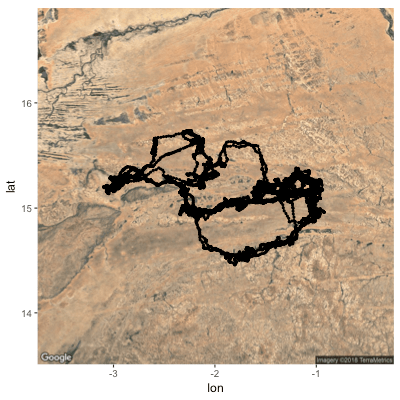
\includegraphics[width=0.49\textwidth]{elephant_plotSat.png}
  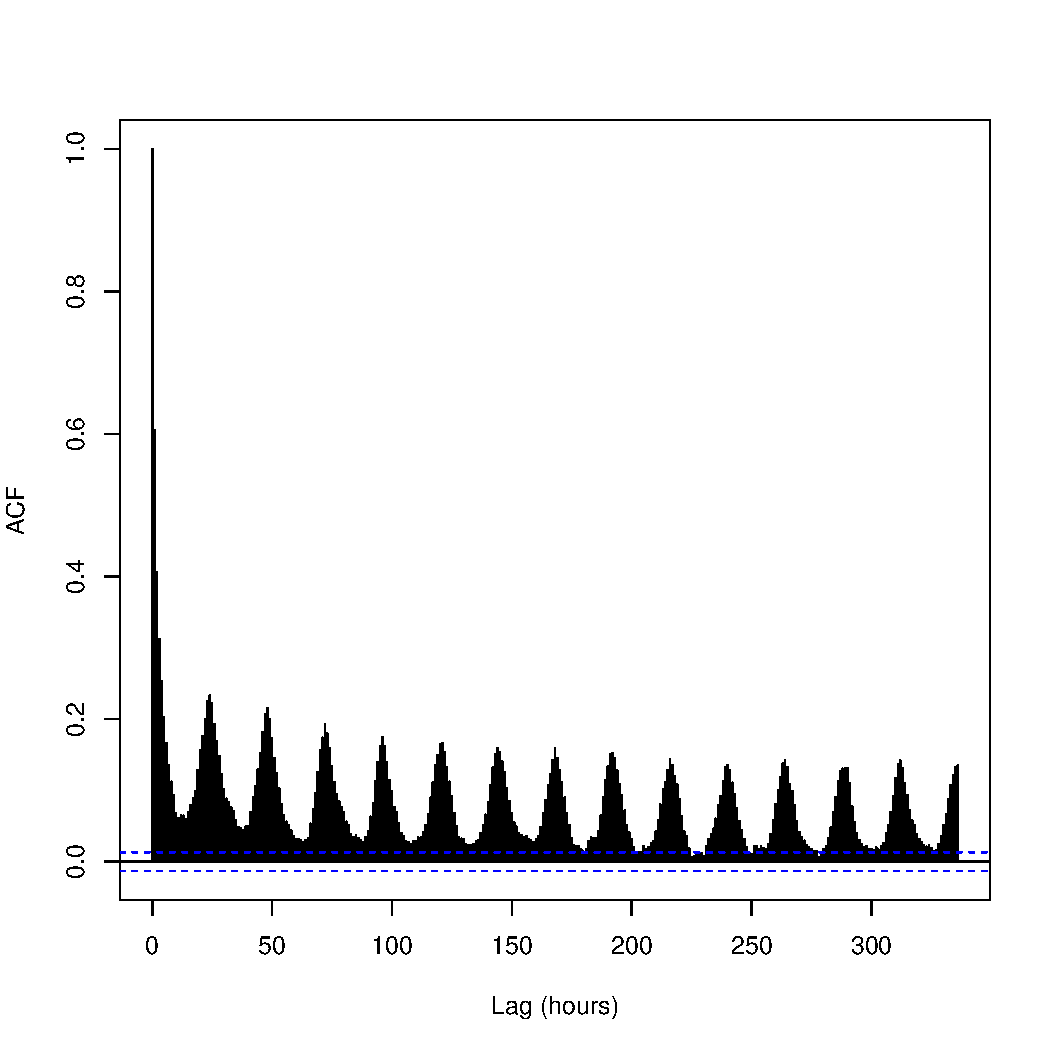
\includegraphics[width=0.49\textwidth]{plot_elephantResults017.pdf}
  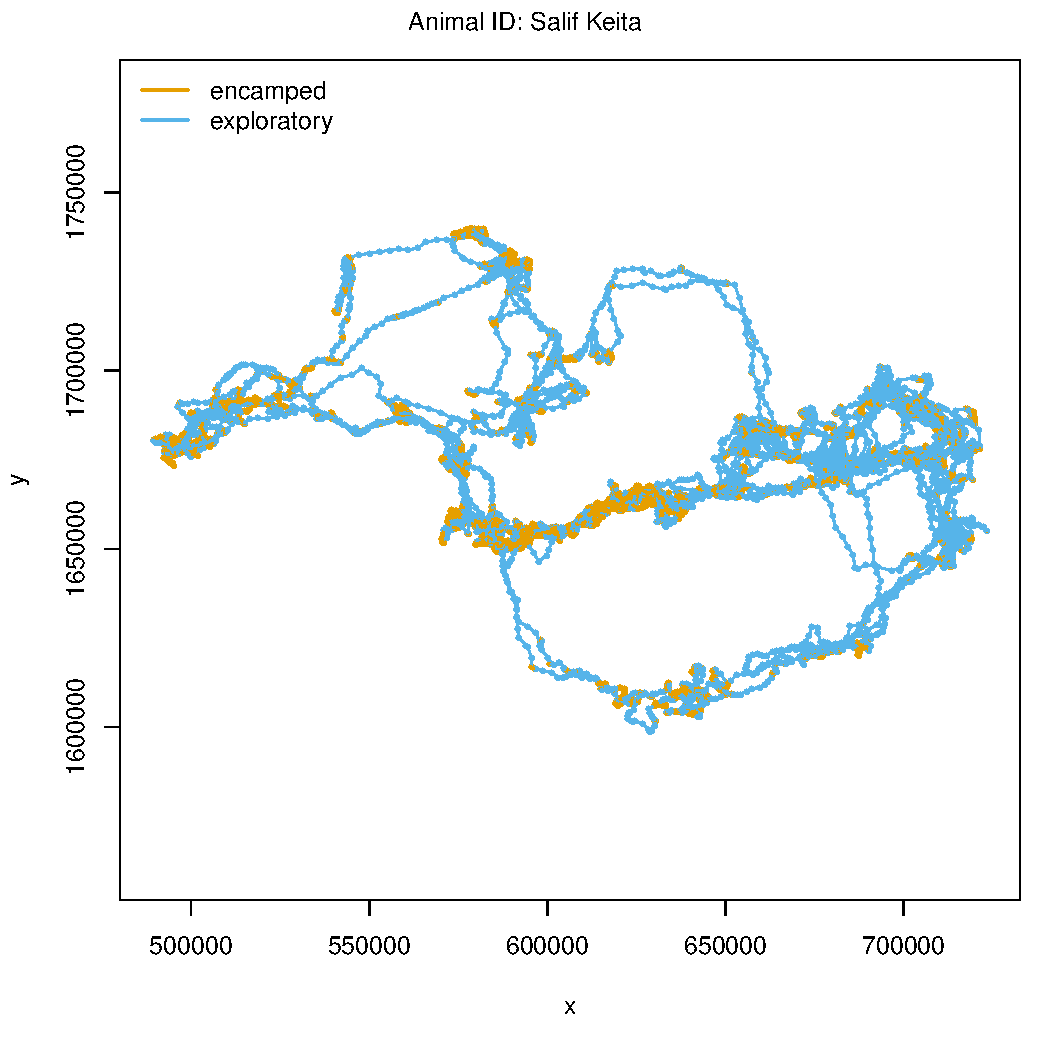
\includegraphics[width=0.49\textwidth]{plot_elephantResults015.pdf}
  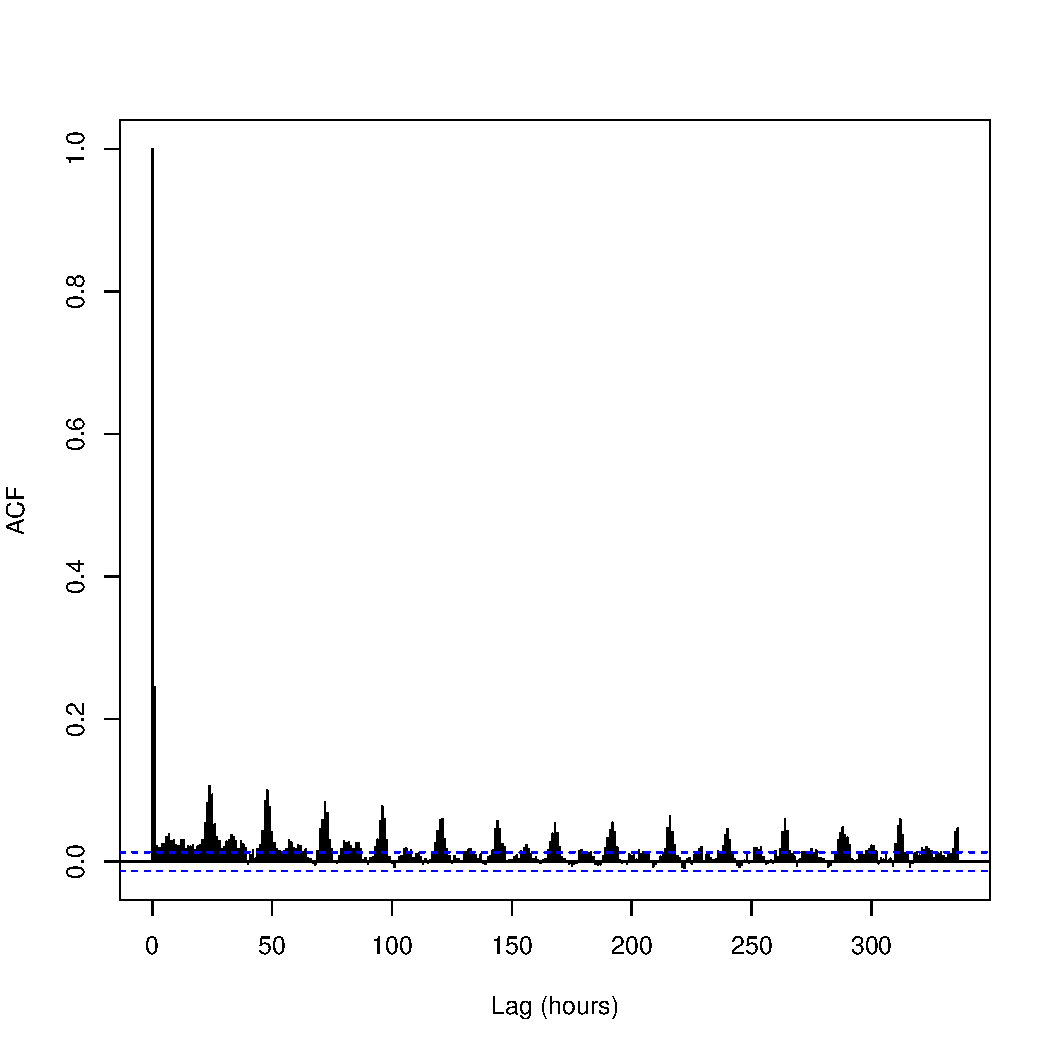
\includegraphics[width=0.49\textwidth]{plot_elephantResults016.pdf}
  \caption{Plot of the elephant track produced using the `plotSat' function (top-left panel), autocorrelation function (ACF) plot of the corresponding step length data (top-right panel), plot of the Viterbi-decoded state sequence for the 2-state (``encamped'' and ``exploratory'') model generated using the generic `plot' function (bottom-left panel), and the step length pseudo-residual ACF plot for this model using the `plotPR' function (bottom-right panel).}
  \label{fig:elephantResults1}
\end{figure}

\begin{figure}[htbp]
  \centering
  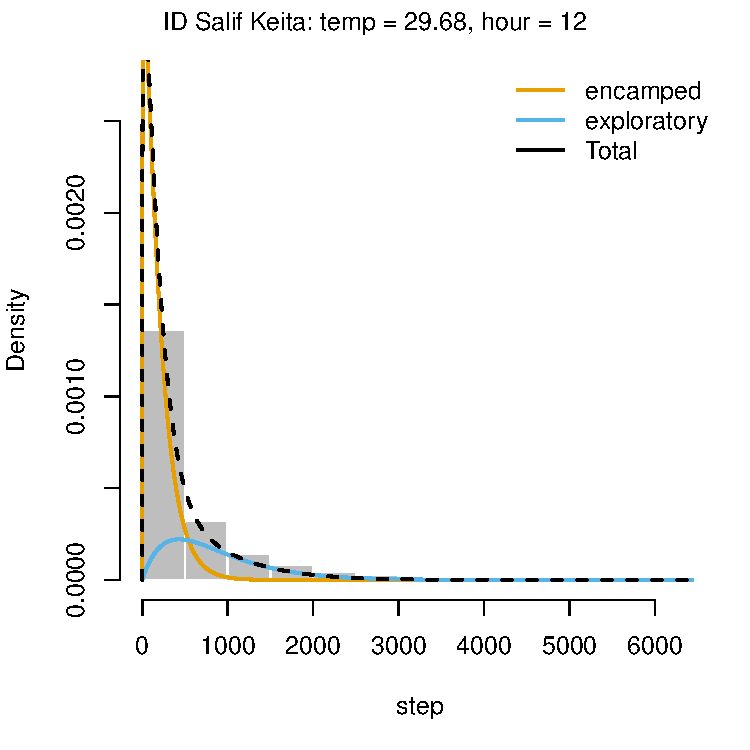
\includegraphics[width=0.35\textwidth]{plot_elephantResults009.pdf}
  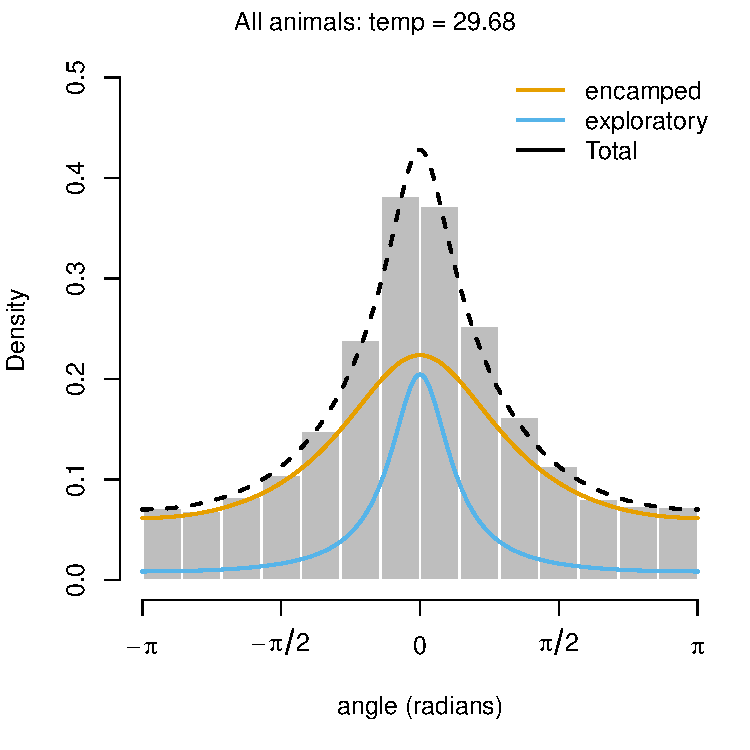
\includegraphics[width=0.35\textwidth]{plot_elephantResults012.pdf} \\
  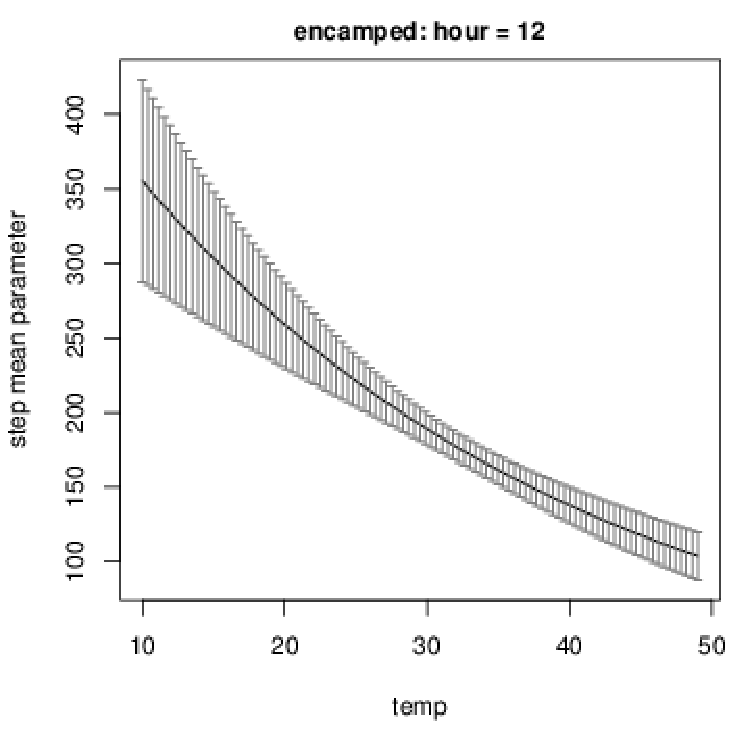
\includegraphics[width=0.35\textwidth]{plot_elephantResults001.pdf} 
  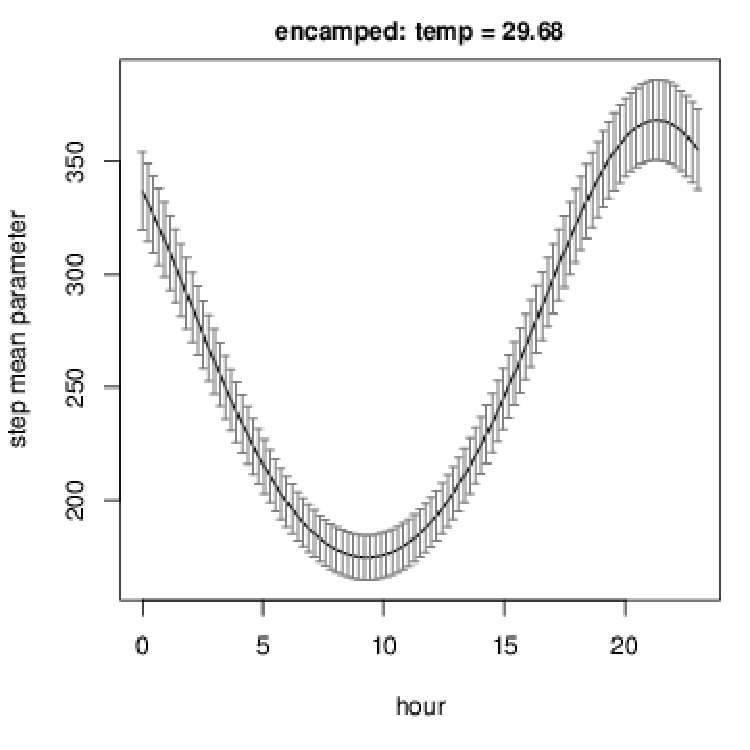
\includegraphics[width=0.35\textwidth]{plot_elephantResults002.pdf} \\
  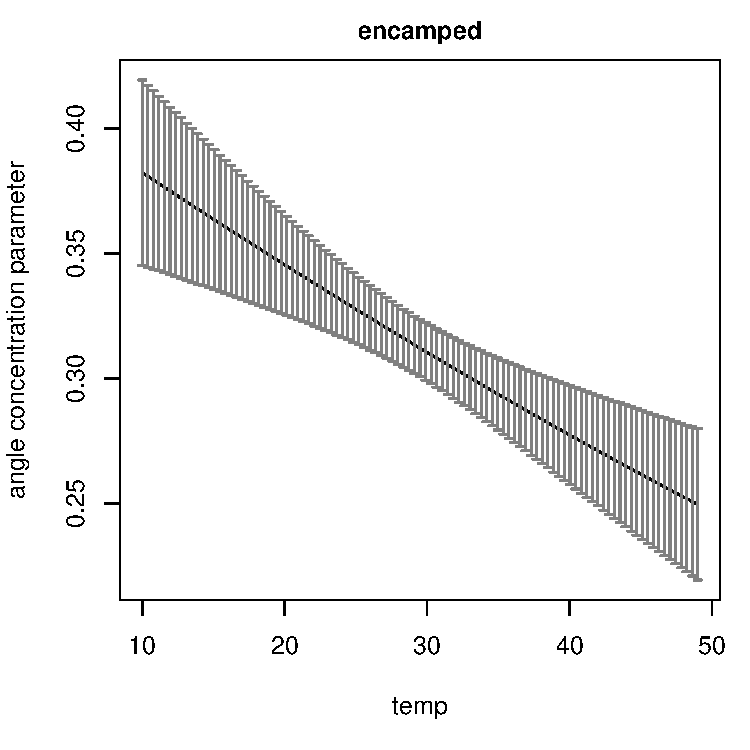
\includegraphics[width=0.35\textwidth]{plot_elephantResults010.pdf}
  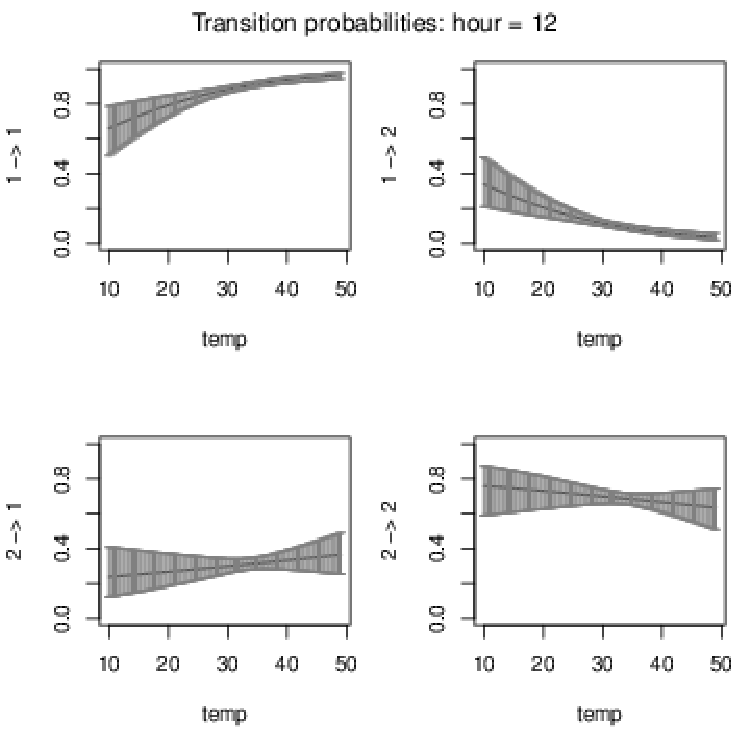
\includegraphics[width=0.35\textwidth]{plot_elephantResults013.pdf} \\
  \caption{Selected plots for the 2-state (``encamped'' and ``exploratory'') African elephant example generated using the generic 'plot' function. Top panels present histograms of the step length (top-left) and turning angle (top-right) data along with the estimated state-dependent probability distributions based on the mean temperature (temp = 29.7 degrees celsius) at 12:00 GMT (hour = 12). Middle panels present estimates (and 95\% confidence intervals) for the step length mean parameter of the ``encamped'' state as a function of temperature and hour of day.  Bottom-left panel presents estimates for the turning angle concentration parameter of the ``encamped'' state as a function of temperature.  Bottom-right panel presents estimated state transition probabilities (1 = ``encamped'', 2 = ``exploratory'') as a function of temperature at 12:00 GMT.}
  \label{fig:elephantResults2}
\end{figure}

\subsection{Northern fur seal}
\label{sec:nfs}
In our second example, we use the northern fur seal ({\it Callorhinus ursinus}) example from \cite{McClintockEtAl2014b} to demonstrate the use of additional data streams for distinguishing behaviors with similar horizontal trajectories in a multivariate HMM. The data consist of 241 temporally-irregular Fastloc GPS locations obtained during a foraging trip of a nursing female near the Pribilof Islands of Alaska, USA, from 10-17 October 2007. The tag included time-depth recording capabilities, and the dive activity data were summarized as the number of foraging dives over $T=228$ temporally-regular 1 hr time steps. To fit the $N=3$ state (1=``resting'', 2=``foraging'', 3=``transit'') of \cite{McClintockEtAl2014b} using \verb|momentuHMM|, we first used \verb|crawlWrap| to predict temporally-regular locations at 1 hr time steps assuming a bivariate normal measurement error model and merged the results with the foraging dive data using the \verb|crawlMerge| function. Then multiple imputation was used to account for location measurement error by repeatedly fitting the HMM to \verb|nSims| realizations of the position process using \verb|MIfitHMM|:% in parallel on \verb|ncores| cores of a (multi-core) processor:
\begin{knitrout}
\definecolor{shadecolor}{rgb}{0.969, 0.969, 0.969}\color{fgcolor}\begin{kframe}
\begin{alltt}
\hlstd{nbStates} \hlkwb{<-} \hlnum{3}
\hlstd{stateNames} \hlkwb{<-} \hlkwd{c}\hlstd{(}\hlstr{"resting"}\hlstd{,} \hlstr{"foraging"}\hlstd{,} \hlstr{"transit"}\hlstd{)}
\hlstd{dist} \hlkwb{<-} \hlkwd{list}\hlstd{(}\hlkwc{step} \hlstd{=} \hlstr{"gamma"}\hlstd{,} \hlkwc{angle} \hlstd{=} \hlstr{"wrpcauchy"}\hlstd{,} \hlkwc{dive} \hlstd{=} \hlstr{"pois"}\hlstd{)}
\hlstd{Par0} \hlkwb{<-} \hlkwd{getParDM}\hlstd{(}\hlkwc{nbStates} \hlstd{= nbStates,} \hlkwc{dist} \hlstd{= dist,}
                 \hlkwc{Par} \hlstd{= Par,} \hlkwc{DM} \hlstd{= DM,} \hlkwc{workBounds} \hlstd{= workBounds,}
                 \hlkwc{estAngleMean} \hlstd{=} \hlkwd{list}\hlstd{(}\hlkwc{angle} \hlstd{=} \hlnum{FALSE}\hlstd{))}
\hlstd{Fixpar} \hlkwb{<-} \hlkwd{list}\hlstd{(}\hlkwc{dive} \hlstd{=} \hlkwd{c}\hlstd{(}\hlopt{-}\hlnum{100}\hlstd{,} \hlnum{NA}\hlstd{,} \hlnum{NA}\hlstd{))}
\hlstd{nfsFits} \hlkwb{<-} \hlkwd{MIfitHMM}\hlstd{(crwOut,} \hlkwc{nSims} \hlstd{=} \hlnum{100}\hlstd{,} \hlkwc{nbStates} \hlstd{= nbStates,} \hlkwc{dist} \hlstd{= dist,}
                    \hlkwc{Par0} \hlstd{= Par0,} \hlkwc{DM} \hlstd{= DM,} \hlkwc{workBounds} \hlstd{= workBounds,}
                    \hlkwc{estAngleMean} \hlstd{=} \hlkwd{list}\hlstd{(}\hlkwc{angle} \hlstd{=} \hlnum{FALSE}\hlstd{),}
                    \hlkwc{fixPar} \hlstd{= fixPar,} \hlkwc{retryFits} \hlstd{=} \hlnum{30}\hlstd{,}
                    \hlkwc{stateNames}\hlstd{=stateNames)}
\hlkwd{plot}\hlstd{(nfsFits)}
\end{alltt}
\end{kframe}
\end{knitrout}
Here we specified a gamma distribution for step length (`step'), wrapped Cauchy distribution for turning angle (`angle'), and Poisson distribution for the number of foraging dives (`dive'). The function \verb|getParDM| was used to organize the starting values for the data stream working parameters (\verb|Par0|) in the correct format based on \verb|DM|, \verb|workBounds|, and estimates of the natural parameters (\verb|Par|) from \cite{McClintockEtAl2014b}. The \verb|DM| and \verb|workBounds| arguments were specified to avoid label switching among the \verb|nSims| imputed data model fits and enforce similar state-dependent probability distribution constraints as \cite{McClintockEtAl2014b}; for example, constraining the Poisson rate parameters such that the ``foraging'' state tends to have higher numbers of foraging dives than the ``transit'' state ($\lambda_2 > \lambda_3$; see Eq. \ref{eq:link} in section \ref{sec:harbourSeal} for more details on parameter constraints using \verb|DM| in conjunction with the \verb|userBounds| and \verb|workBounds| arguments). To prohibit foraging dives for the ``resting'' state, we used the \verb|fixPar| argument to effectively fix the Poisson rate parameter to zero on the natural scale (i.e. $\lambda_1 \approx 0$).  To help deal with the problem of convergence to local maxima, the \verb|retryFits| argument allows users to specify the number of times to attempt to re-fit each model using random perturbations of the parameter estimates as the starting values for optimization.

The results are very similar to those of the discrete-time model of \cite{McClintockEtAl2014b}, with periods of foraging often followed by resting (Figure \ref{fig:nfsResults}).  The ``activity budgets'' (i.e. the proportion of time steps allocated to each state) calculated by \verb|MIpool| based on the estimated state sequences for each imputation were 0.31 (95\% CI: 0.25$-$0.37) for ``resting'', 0.28 (95\% CI: 0.23$-$0.35) for ``foraging'', and 0.41 (95\% CI: 0.33$-$0.5) for ``transit''.

\begin{figure}[htbp]
  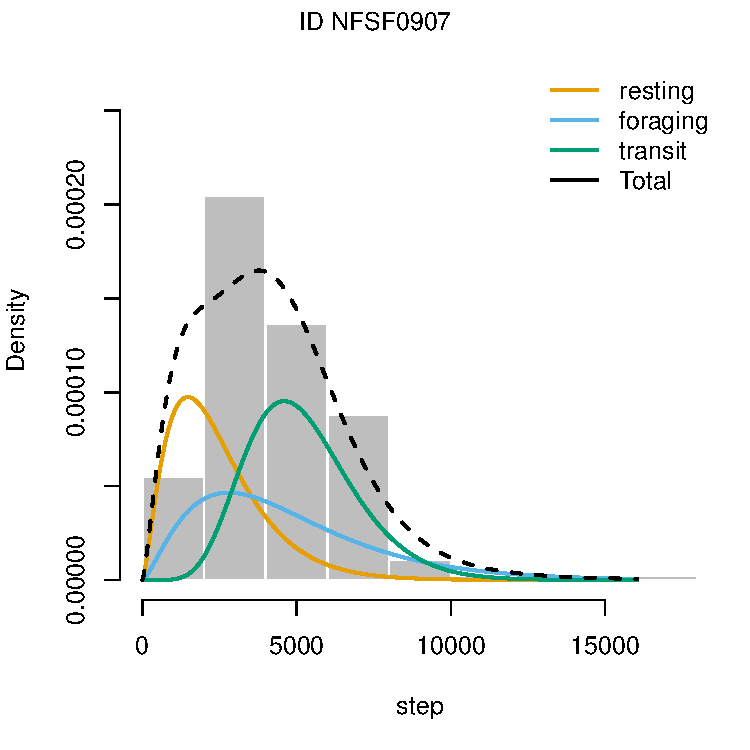
\includegraphics[width=0.49\textwidth,page=1]{plot_nfsResults}
  \includegraphics[width=0.49\textwidth,page=2]{plot_nfsResults}
  \includegraphics[width=0.49\textwidth,page=3]{plot_nfsResults}
  \includegraphics[width=0.49\textwidth,page=4]{plot_nfsResults}
  \caption{Plots of the northern fur seal example results generated using the generic `plot' function. The estimated probability distributions for step length (top-left panel), turning angle (top-right panel), and number of foraging dives (bottom-left panel) for the 3-state (``resting'', ``foraging'', and ``transit'') model are plotted along with histograms of these data streams. The temporally-regular predicted locations (and 95\% ellipsoidal confidence bands) and estimated states are plotted in the bottom-right panel. All estimates are pooled across multiple imputations of the position process and thus reflect uncertainty attributable to location measurement error and temporally-irregular observations.}
  \label{fig:nfsResults}
\end{figure}
\subsection{Loggerhead turtle}
\label{sec:turtle}
For our third example, we demonstrate how to model movement direction and step length as a function of angular covariates using hitherto unpublished loggerhead turtle ({\it Caretta caretta}) data for a captive-raised juvenile released in 2012 on the coast of North Carolina, USA. The data consist of 165 temporally-irregular Argos locations subject to measurement error and rasters of daily ocean surface currents collected between 20 November and 19 December 2012. Assuming a gamma distribution for step length $(l_t)$ and a wrapped Cauchy distribution for turning angle $(\phi_t)$, we model the mean step length parameter $(\mu^l_t)$ as a function of ocean surface current speed $(w_t)$ and direction $(r_t)$ relative to the bearing of movement $(b_t)$:
\begin{equation}
  \mu^l_t=\exp(\beta^l_0+\beta^l_1 w_t \cos(b_t-r_t)),
  \label{eq:turtleMeanStep}
\end{equation}
%or, equivalently,
%\begin{equation}
%  \mu^l_t=\exp(\beta^l_0+\beta^l_1 w_t \cos(\phi_t-d_t))
%  \label{eq:turtleMeanStep}
%\end{equation}
and the turning angle mean parameter $(\mu^\phi_t)$ as a trade-off between short-term directional persistence and bias in the direction of ocean surface currents using the circular-circular regression link function:
\begin{equation}
  \mu^\phi_t=\text{atan2}(\sin(d_t) \beta^\phi,1+\cos(d_t)\beta^\phi),
    \label{eq:turtleMeanAngle}
\end{equation}
where $d_t=\text{atan2}(\sin(r_t-b_{t-1}),\cos(r_t-b_{t-1}))$.

We wish to fit a 2-state HMM to the turtle data, with a ``foraging'' state unaffected by currents and a ``transit'' state potentially influenced by ocean surface currents as in Eqs. \ref{eq:turtleMeanStep} and \ref{eq:turtleMeanAngle}.  We used \verb|crawlWrap| to predict $T=350$ temporally-regular locations at 2 hr time steps assuming a bivariate normal measurement error model that accounts for the Argos location quality class  (i.e. 3,2,1,0,A,B) of each observation. We then again used multiple imputation to account for location uncertainty by repeatedly fitting the HMM to \verb|nSims| realizations of the position process using \verb|MIfitHMM|. We first draw \verb|nSims| realizations of the position process and extract the corresponding spatial covariates from the raster bricks for ocean surface current speed (``speedBrick'') and direction (``dirBrick'') using \verb|MIfitHMM| with \verb|fit=FALSE|:
\begin{knitrout}
\definecolor{shadecolor}{rgb}{0.969, 0.969, 0.969}\color{fgcolor}\begin{kframe}
\begin{alltt}
\hlstd{miTurtleData} \hlkwb{<-} \hlkwd{MIfitHMM}\hlstd{(crwOut,} \hlkwc{nSims} \hlstd{=} \hlnum{100}\hlstd{,} \hlkwc{fit}\hlstd{=}\hlnum{FALSE}\hlstd{,}
                 \hlkwc{spatialCovs} \hlstd{=} \hlkwd{list}\hlstd{(}\hlkwc{w} \hlstd{= speedBrick,} \hlkwc{d} \hlstd{= dirBrick,} \hlkwc{r} \hlstd{= dirBrick),}
                 \hlkwc{angleCovs} \hlstd{=} \hlstr{"d"}\hlstd{)}
\end{alltt}
\end{kframe}
\end{knitrout}
When the \verb|fit| argument is \verb|FALSE|, \verb|MIfitHMM| returns a list of length \verb|nSims| composed of \verb|momentuHMMData| objects (\verb|miData|). For convenience and ease of interpretation, we manually added an additional covariate $\left({\text angle\_osc}=\cos(b_t-r_t)\right)$ to each of the imputed data sets and fitted the 2-state HMM using Eqs. \ref{eq:turtleMeanStep} and \ref{eq:turtleMeanAngle} for state 2 (``transit''):
%<<prep-turtle, echo=TRUE, eval=FALSE>>=
%for(j in 1:30){
%  miTurtleData$miData[[j]]$angle_osc <- miTurtleData$miData[[j]]$angle
%                                        -miTurtleData$miData[[j]]$osc_dir
%}
%@
%Now the imputed data are ready to be fitted to the 2-state HMM using Eqs. \ref{eq:turtleMeanStep} and \ref{eq:turtleMeanAngle} for state 2 (``transit''):
\begin{knitrout}
\definecolor{shadecolor}{rgb}{0.969, 0.969, 0.969}\color{fgcolor}\begin{kframe}
\begin{alltt}
\hlstd{nbStates}\hlkwb{<-}\hlnum{2}
\hlstd{dist} \hlkwb{<-} \hlkwd{list}\hlstd{(}\hlkwc{step} \hlstd{=} \hlstr{"gamma"}\hlstd{,} \hlkwc{angle} \hlstd{=} \hlstr{"wrpcauchy"}\hlstd{)}
\hlstd{DM} \hlkwb{<-} \hlkwd{list}\hlstd{(}\hlkwc{step} \hlstd{=} \hlkwd{list}\hlstd{(}\hlkwc{mean} \hlstd{=} \hlopt{~}\hlkwd{state2}\hlstd{(w}\hlopt{:}\hlstd{angle_osc),} \hlkwc{sd} \hlstd{=} \hlopt{~}\hlnum{1}\hlstd{),}
           \hlkwc{angle} \hlstd{=} \hlkwd{list}\hlstd{(}\hlkwc{mean} \hlstd{=} \hlopt{~}\hlkwd{state2}\hlstd{(d),} \hlkwc{concentration}\hlstd{=} \hlopt{~}\hlnum{1}\hlstd{))}
\hlstd{turtleFits} \hlkwb{<-} \hlkwd{MIfitHMM}\hlstd{(miTurtleData}\hlopt{$}\hlstd{miData,} \hlkwc{nbStates} \hlstd{= nbStates,} \hlkwc{dist} \hlstd{= dist,}
                       \hlkwc{Par0} \hlstd{= Par0,} \hlkwc{DM} \hlstd{= DM,}
                       \hlkwc{estAngleMean} \hlstd{=} \hlkwd{list}\hlstd{(}\hlkwc{angle} \hlstd{=} \hlnum{TRUE}\hlstd{),}
                       \hlkwc{circularAngleMean} \hlstd{=} \hlkwd{list}\hlstd{(}\hlkwc{angle} \hlstd{=} \hlnum{TRUE}\hlstd{))}
\hlkwd{plot}\hlstd{(turtleFits,} \hlkwc{plotCI} \hlstd{=} \hlnum{TRUE}\hlstd{,} \hlkwc{covs} \hlstd{=} \hlkwd{data.frame}\hlstd{(}\hlkwc{angle_osc} \hlstd{=} \hlkwd{cos}\hlstd{(}\hlnum{0}\hlstd{)))}
\end{alltt}
\end{kframe}
\end{knitrout}
Note that the \verb|state2| special function in \verb|DM| indicates the covariate formulas are specific to state 2 (``transit'') and the \verb|circularAngleMean| argument indicates that circular-circular regression link function is to be used on the mean turning angle parameter as in Eq. \ref{eq:turtleMeanAngle}. 

For the ``transit'' state, pooled parameter estimates indicated step lengths increased with ocean surface current speed and as the bearing of movement aligned with ocean surface current direction ($\beta^l_1=0.4, \text{95\% CI: } 0.09-0.7$; Figure \ref{fig:turtleResults}). The estimated wrapped Cauchy distribution for turning angle had mean angles $(\mu^\phi_t)$ biased towards the direction of ocean surface currents for each time step $(\beta^\phi=0.26, \text{95\% CI: } 0.04-0.48)$, with concentration parameter $\rho^\phi_2=0.86$ (95\% CI: 0.82$-$0.9) indicating turning angles were concentrated at $\mu^\phi_t$. Thus movement during the ``transit'' state appears to strongly follow ocean surface currents (mean ${\text angle\_osc}=0.88,{\text SD}=0.22$), while movement during the ``foraging'' state exhibited shorter step lengths $(\mu^l_1=3001{\text m}, \text{95\% CI: } 2439-3563)$ perpendicular to ocean surface currents (mean ${\text angle\_osc}=0.07,{\text SD}=0.27$), with some directional persistence $(\rho^\phi_1=0.49, \text{95\% CI: } 0.37-0.61)$. The turtle spent 0.56 (95\% CI: 0.46$-$0.66) of the 2 hr time steps in the ``foraging'' state and 0.44 (95\% CI: 0.34$-$0.54) of time steps in the ``transit'' state as it travelled northeast along a predominant current until it (presumably) found an attractive foraging patch (Figure \ref{fig:turtleResults}).

\begin{figure}[htbp]
  \centering
  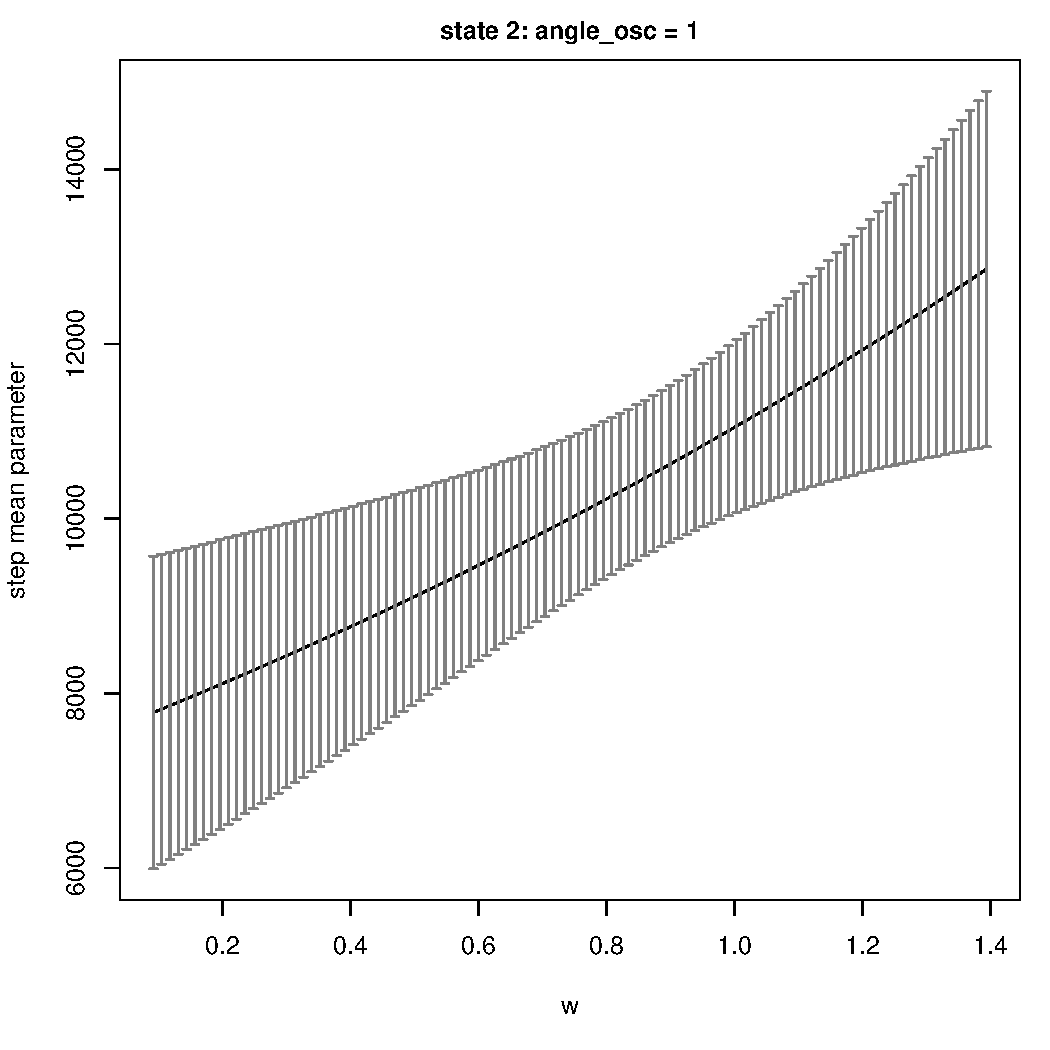
\includegraphics[width=0.32\textwidth]{plot_turtleResults001.pdf}
  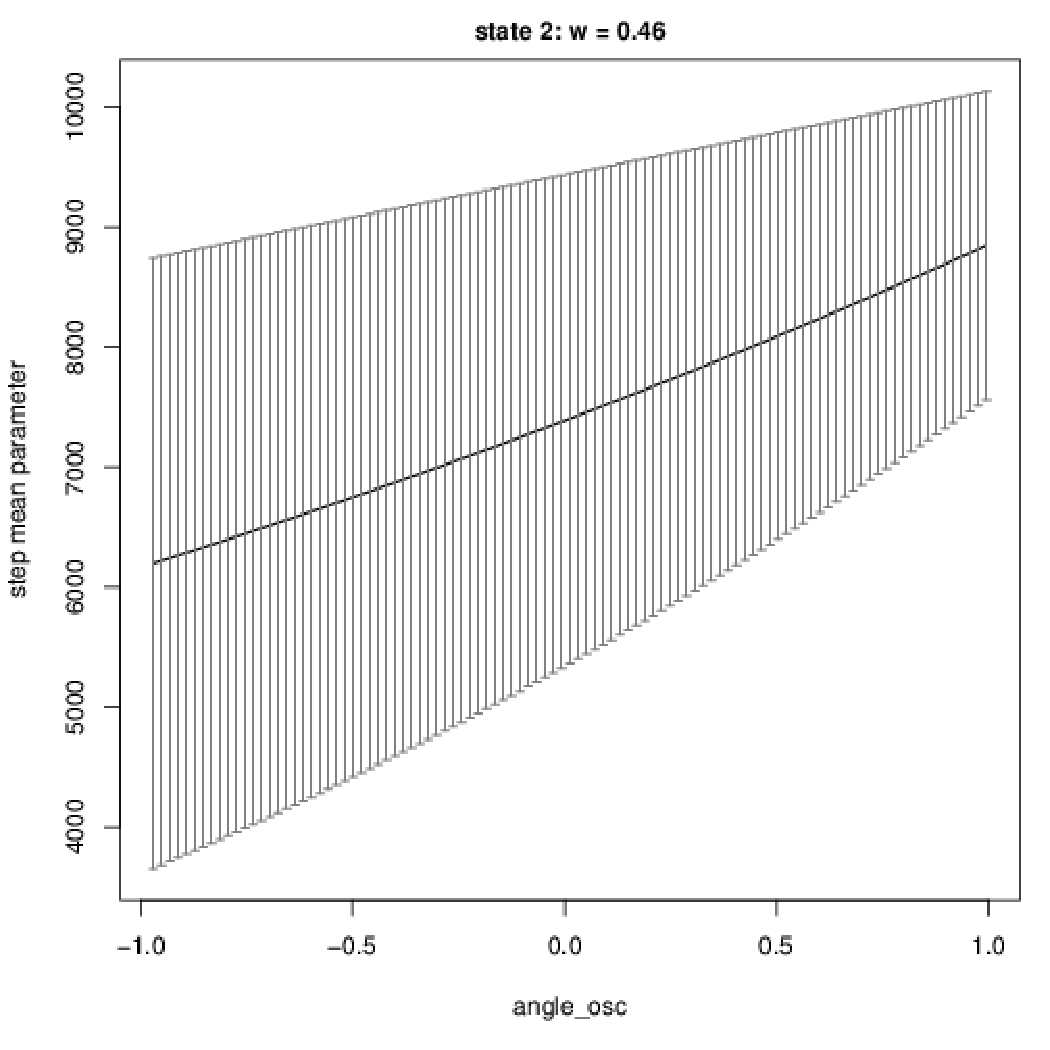
\includegraphics[width=0.32\textwidth]{plot_turtleResults002.pdf}
  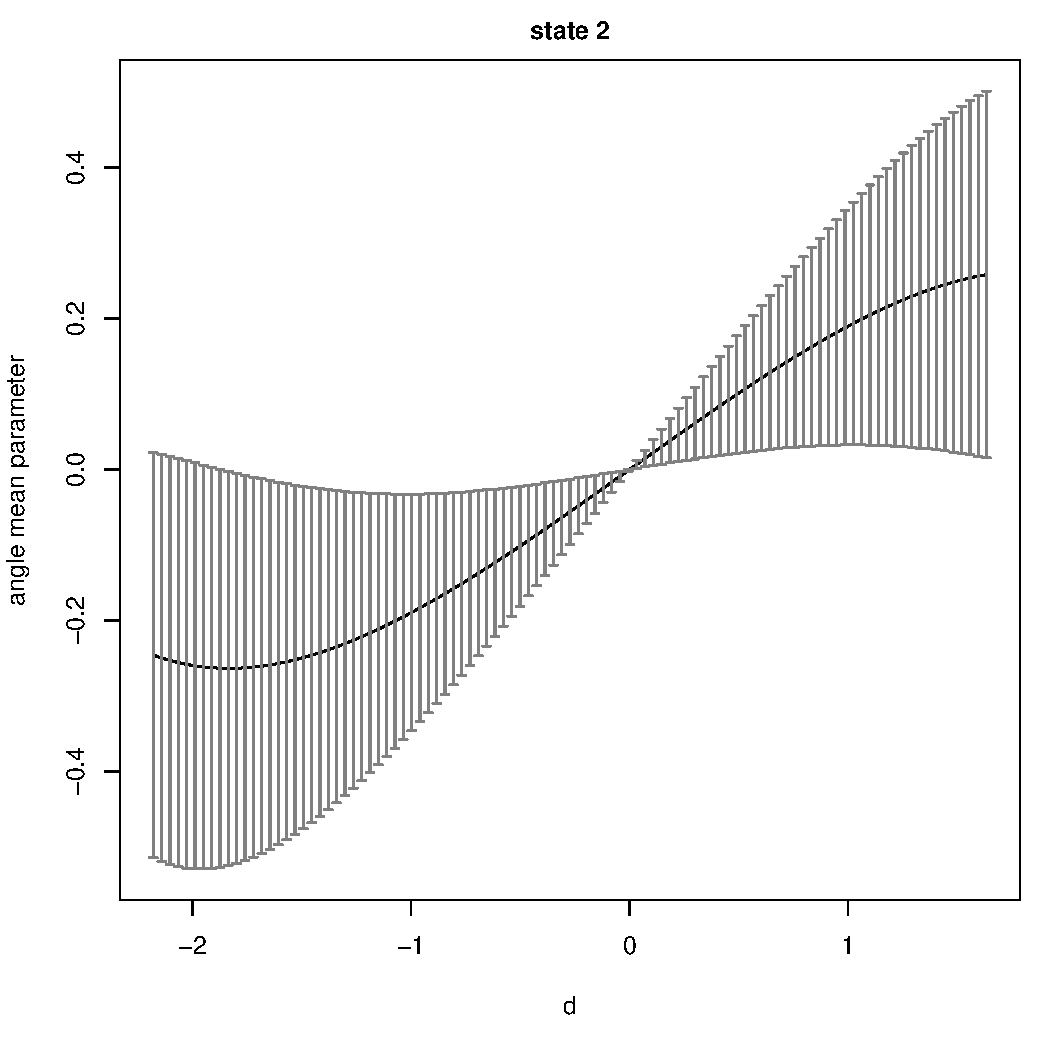
\includegraphics[width=0.32\textwidth]{plot_turtleResults004.pdf}
  %\begin{adjustbox}{trim=0cm 0.25cm 0cm 1.5cm}
    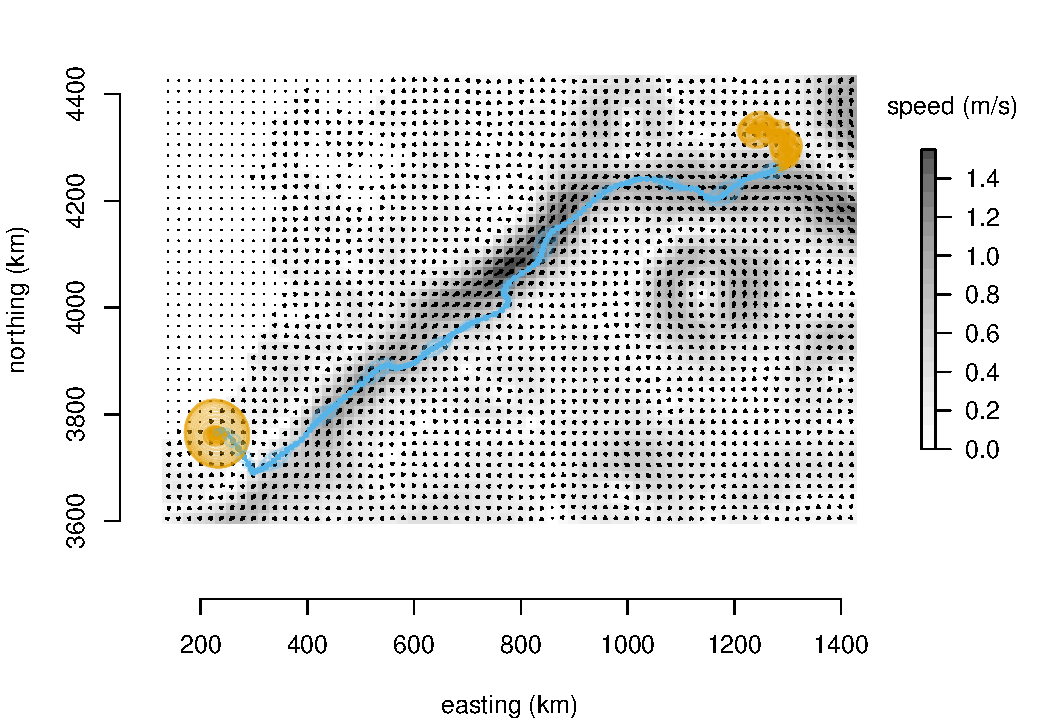
\includegraphics[width=\textwidth]{plot_turtleResults2.pdf}
  %\end{adjustbox}
  \caption{Selected results from the loggerhead turtle example. Top panels include estimates and 95\% confidence intervals for the mean step length parameter as a function of ocean surface current speed $(w)$ when ocean surface current direction $(r_t)$ is the same as the bearing $(b_t)$ of movement (i.e. ${\text angle\_osc}=\cos(b_t-r_t)=1$; top-left panel), mean step length parameter as a function of ${\text angle\_osc}$ at the mean ocean surface current speed ($w=0.46$ m/s; top-middle panel), and mean turning angle parameter as a function of $d_t=\text{atan2}(\sin(r_t-b_{t-1}),\cos(r_t-b_{t-1}))$ (top-right panel). Bottom panel plots the pooled track, 95\% error ellipse confidence bands, and state (orange = ``foraging'', blue = ``transit'') estimates based on multiple imputations of the position process relative to ocean surface current speed (m/s) and direction on 2 December 2012.}
  \label{fig:turtleResults}
\end{figure}

It may often make more sense to weight angular covariates (such as ocean surface current direction) by their relative strength or importance. For example, weak ocean surface currents may be less likely to influence movement direction than strong ocean surface currents. This could easily be included in our turtle model using the \verb|angleFormula(cov, strength, by)| special function in \verb|DM|, where \verb|cov| is an angle covariate (e.g. wind direction), \verb|strength| is an optional positive real covariate (e.g. wind speed), and \verb|by| is an optional factor variable for individual- or group-level effects (e.g. ID, sex):
\begin{knitrout}
\definecolor{shadecolor}{rgb}{0.969, 0.969, 0.969}\color{fgcolor}\begin{kframe}
\begin{alltt}
\hlstd{DM}\hlopt{$}\hlstd{angle} \hlkwb{=} \hlkwd{list}\hlstd{(}\hlkwc{mean} \hlstd{=} \hlopt{~}\hlkwd{state2}\hlstd{(}\hlkwd{angleFormula}\hlstd{(d,} \hlkwc{strength} \hlstd{= w)),}
                \hlkwc{concentration}\hlstd{=} \hlopt{~}\hlnum{1}\hlstd{)}
\end{alltt}
\end{kframe}
\end{knitrout}
\noindent which would yield the following model for the ``transit'' state mean angle parameter:
\begin{equation}
  \mu^\phi_t=\text{atan2}(w_t \sin(d_t) \beta^\phi,1+w_t \cos(d_t)\beta^\phi).
    \label{eq:turtleMeanAngle2}
\end{equation}

Still another option would be to use the von Mises consensus model, where the concentration parameter would now depend on the level of agreement between short-term directional persistence (i.e. going forward) and ocean surface currents: 
\begin{knitrout}
\definecolor{shadecolor}{rgb}{0.969, 0.969, 0.969}\color{fgcolor}\begin{kframe}
\begin{alltt}
\hlstd{dist}\hlopt{$}\hlstd{angle} \hlkwb{=} \hlstr{"vmConsensus"}
\hlstd{DM}\hlopt{$}\hlstd{angle} \hlkwb{=} \hlkwd{list}\hlstd{(}\hlkwc{mean} \hlstd{=} \hlopt{~}\hlkwd{state2}\hlstd{(}\hlkwd{angleFormula}\hlstd{(d,} \hlkwc{strength} \hlstd{= w)),}
                \hlkwc{kappa} \hlstd{=} \hlopt{~}\hlnum{1}\hlstd{)}
\end{alltt}
\end{kframe}
\end{knitrout}
\noindent which would yield the following model for the ``transit'' state concentration parameter:
\begin{equation}
  \rho^\phi_t = \kappa \sqrt{[w_t \sin(d_t) \beta^\phi]^2+[1+w_t \cos(d_t)\beta^\phi]^2}.
    \label{eq:turtleMeanAngle3}
\end{equation}
If there were multiple turtles in this dataset, then individual-level effects could be included on $\mu^\phi$ by simply specifying \verb|angleFormula(d, strength = w, by = ID)| or \verb|angleFormula(d, by = ID)| (with no strength effects).

One disadvantage of modeling steps and turns as above is that the fitted model cannot be properly simulated using \verb|simData|. This is because \verb|simData| is unable to calculate new realizations of the constructed covariate $\left({\text angle\_osc}=\cos(b_t-r_t)\right)$. However, we can implement a very similar model on the positions directly using a bivariate normal random walk.  While arguably more intuitive, modeling the positions directly also has the added benefit that the fitted model can be properly simulated using \verb|simData|. Similar to the continuous-time potential function approach of \cite{BrillingerEtAl2012} and \cite{HootenEtAl2019}, we can model the positions ${\boldsymbol \mu}=(\mu_x, \mu_y)$ as a bivariate normal random walk where the position at time $t$ is a function of the position at time $t-1$ and the ocean surface current velocity vectors $V({\boldsymbol \mu}_{t-1})=(u_{t-1},v_{t-1})$, where $u$ is easting and $v$ is northing:
\begin{eqnarray}
%(x_t, y_t) \sim N \left( (\mu_{x,t},\mu_{y,t}),\Sigma \right),
\label{eq:potFun}
{\boldsymbol \mu}_t \mid S_t = s \sim {\mathcal N} \left({\boldsymbol \mu}_{t-1}+({\boldsymbol \mu}_{t-1}-{\boldsymbol \mu}_{t-2})\beta_1 + V({\boldsymbol \mu}_{t-1})\beta_2 I(s=2),\sigma_s^2 {\mathbf I} \right),
\end{eqnarray}
%where
%\begin{eqnarray}
% \label{eq:potFun}
%\mu_{x,t} &=& x_{t-1}+(x_{t-1}-x_{t-2}) \beta_1 + u_{t-1} \beta_2, \nonumber \\
%\mu_{y,t} &=& y_{t-1}+(y_{t-1}-y_{t-2}) \beta_1 + v_{t-1} \beta_2, 
%\end{eqnarray}
%and 
%\begin{equation*}
%  \Sigma = \begin{bmatrix}
%            \sigma_x^2    & 0    \\
%                     0    & \sigma_y^2        
%  \end{bmatrix}
%\end{equation*}
where $I()$ is the indicator function and $\mathbf I$ is a $2 \times 2$ identity matrix. %This is analogous to state 2 in our model for steps and turns, where the terms $(x_{t-1}-x_{t-2})$ and $(y_{t-1}-y_{t-2})$ account for persistence in velocity. For state 1 we would simply remove the terms related to ocean surface current velocities ($u_t$ and $v_t$). 
This is analogous to our model for steps and turns, where $({\boldsymbol \mu}_{t-1}-{\boldsymbol \mu}_{t-2})$ accounts for persistence in velocity. Thus when in state 1 (i.e., $S_t=1$) the movement model is a correlated random walk, but when in state 2 (i.e., $S_t=2$) the movement model includes a potential function surface based on ocean surface currents.

Recall that multivariate normal distributions require some additonal book-keeping when preparing the data; the \verb|altCoordNames| argument in \verb|prepData| and \verb|MIfitHMM| and the \verb|mvnCoords| argument in \verb|fitHMM| and \verb|MIfitHMM| are designed to help properly format and identify multivariate coordinate data streams. For example, if a bivariate normal data stream name is ``loc'' (e.g. \verb|dist=list(loc="mvnorm2")|), then the data must include columns ``loc.x'' and ''loc.y'' for the x- and y- coordinates, respectively.  When using a multivariate normal random walk distribution, the previous position can be referenced in \verb|DM| formulas or pseudo-design matrices. For example, for a bivariate normal random walk data stream named ``mu'' (e.g. \verb|dist=list(mu="rw_mvnorm2")|), the previous position can be refereced in \verb|DM| as ``mu.x\_tm1'' and ``mu.y\_tm1''. This allows for persistence in velocity to be included as in Eq. \ref{eq:potFun} via the special formula function \verb|crw(x_tm1,lag)|, where argument \verb|x_tm1| is the previous position (e.g. ``mu.x\_tm1'' or ``mu.y\_tm1'') and argument \verb|lag| specifies the time lag for the persistence (\verb|lag=1| in this example, but higher order lags could also be included). A complete demonstration of how to implement this bivariate normal random walk model can be found in the ``turtleExample\_rw\_mvnorm2.R'' script in the \verb|momentuHMM| ``vignettes'' source directory (or at \url{https://github.com/bmcclintock/momentuHMM}).

\subsection{Grey seal}
\label{sec:greySeal}
For our next example, we perform a similar analysis of a grey seal ({\it Halichoerus grypus}) track that was originally conducted by \cite{McClintockEtAl2012} using Bayesian methods and (computationally-intensive) Markov chain Monte Carlo. The data consist of 1045 temporally-irregular Fastloc GPS locations collected in the North Sea between 9 April and 11 August 2008. Because the seal repeatedly visited the same haul-out and foraging locations, it provides a nice example for demonstrating how to implement biased movements relative to activity centers using \verb|momentuHMM|. \cite{McClintockEtAl2012} fitted a 5-state model to these data that included three center of attraction states, with movement biased towards two haul-out sites (``Abertay'' and ``Farne Islands'') and a foraging area (``Dogger Bank''), and two ``exploratory'' states (''low speed'', ''high speed'') that were unassociated with an activity center. After using \verb|crawlWrap| to predict $T=1515$ temporally-regular locations at 2 hr time steps including a bivariate normal measurement error model, we can perform a very similar analysis to \cite{McClintockEtAl2012} in \verb|momentuHMM| by using the \verb|centers| argument and state-specific functions for the probability distribution parameters. A cluster analysis on the observed locations using the R package \verb|dtwclust| \citep{SardaEspinosa2017} identified three centroids with coordinates that were nearly identical to the three activity centers (``Abertay'', ``Farne Islands'', and ``Dogger Bank'') identified by \cite{McClintockEtAl2012}. We use these coordinates to derive covariates relative to the activity centers when drawing \verb|nSims| realizations of the position process:
\begin{knitrout}
\definecolor{shadecolor}{rgb}{0.969, 0.969, 0.969}\color{fgcolor}\begin{kframe}
\begin{alltt}
\hlstd{crwSim} \hlkwb{<-} \hlkwd{MIfitHMM}\hlstd{(crwOut,} \hlkwc{nSims} \hlstd{=} \hlnum{100}\hlstd{,} \hlkwc{fit}\hlstd{=}\hlnum{FALSE}\hlstd{,}
                  \hlkwc{center} \hlstd{= centers)}
\end{alltt}
\end{kframe}
\end{knitrout}
Specifying the \verb|centers| argument results in the calculation of two covariates for each activity center: the distance (with `.dist' suffix) and angle (with `.angle' suffix) from each location at time $t$. These covariates can then be used to model parameters as a function of the distance and angle to activity centers for each time step:
\begin{knitrout}
\definecolor{shadecolor}{rgb}{0.969, 0.969, 0.969}\color{fgcolor}\begin{kframe}
\begin{alltt}
\hlstd{dist} \hlkwb{<-} \hlkwd{list}\hlstd{(}\hlkwc{step} \hlstd{=} \hlstr{"weibull"}\hlstd{,} \hlkwc{angle} \hlstd{=} \hlstr{"wrpcauchy"}\hlstd{)}
\hlstd{distFormula} \hlkwb{<-} \hlopt{~}\hlkwd{state1}\hlstd{(}\hlkwd{I}\hlstd{(Abertay.dist}\hlopt{>}\hlnum{2500}\hlstd{))} \hlopt{+} \hlkwd{state2}\hlstd{(}\hlkwd{I}\hlstd{(Farne.dist}\hlopt{>}\hlnum{2500}\hlstd{))}
                  \hlopt{+} \hlkwd{state3}\hlstd{(}\hlkwd{I}\hlstd{(Dogger.dist}\hlopt{>}\hlnum{15000}\hlstd{))}
\hlstd{angleFormula} \hlkwb{<-} \hlopt{~}\hlkwd{state1}\hlstd{(Abertay.angle)} \hlopt{+} \hlkwd{state2}\hlstd{(Farne.angle)}
                  \hlopt{+} \hlkwd{state3}\hlstd{(Dogger.angle)}
\hlstd{stepDM} \hlkwb{<-} \hlkwd{list}\hlstd{(}\hlkwc{shape} \hlstd{= distFormula,} \hlkwc{scale} \hlstd{= distFormula)}
\hlstd{angleDM} \hlkwb{<-} \hlkwd{list}\hlstd{(}\hlkwc{mean} \hlstd{= angleFormula,} \hlkwc{concentration} \hlstd{= distFormula)}
\hlstd{DM} \hlkwb{<-} \hlkwd{list}\hlstd{(}\hlkwc{step} \hlstd{= stepDM,} \hlkwc{angle} \hlstd{= angleDM)}
\end{alltt}
\end{kframe}
\end{knitrout}
Similar to \cite{McClintockEtAl2012}, we assume a Weibull distribution for step length where both the shape and scale parameter depend on the distance from the location at time $t$ to each activity center. For the activity centers on land (``Abertay'' and ``Farne''), we allow the (state-dependent) step length parameters to change when the seal is beyond 2500m of the haulout. For the ``Dogger'' activity center, we allow the parameters to change when the seal is beyond 15000m of this (presumably) foraging area. We thus allow the movement behavior to change within these activity center states upon entering or leaving the vicinity of these sites.  We assume a wrapped Cauchy distribution for turning angle with (state-dependent) mean angle derived from the direction to each activity center at time $t$, and the concentration parameter is modeled similarly to the step length parameters. For the two ``exploratory'' states, we assumed they are simple random walks unaffected by proximity to activity centers. To complete our model specification, we use the \verb|knownStates| argument to assign the seal to the corresponding activity center state whenever it was within the 2500m (haul-out area) or 15000m (foraging area) thresholds for each imputed data set:
\begin{knitrout}
\definecolor{shadecolor}{rgb}{0.969, 0.969, 0.969}\color{fgcolor}\begin{kframe}
\begin{alltt}
\hlstd{greySealFits} \hlkwb{<-} \hlkwd{MIfitHMM}\hlstd{(miDat,} \hlkwc{nSims} \hlstd{=} \hlnum{400}\hlstd{,}
                         \hlkwc{nbStates} \hlstd{=} \hlnum{5}\hlstd{,} \hlkwc{dist} \hlstd{= dist,}
                         \hlkwc{Par0} \hlstd{= Par0,} \hlkwc{beta0} \hlstd{= beta0,} \hlkwc{fixPar} \hlstd{= fixPar,}
                         \hlkwc{formula} \hlstd{= distFormula,}
                         \hlkwc{estAngleMean} \hlstd{=} \hlkwd{list}\hlstd{(}\hlkwc{angle}\hlstd{=}\hlnum{TRUE}\hlstd{),}
                         \hlkwc{circularAngleMean} \hlstd{=} \hlkwd{list}\hlstd{(}\hlkwc{angle}\hlstd{=}\hlnum{0}\hlstd{),}
                         \hlkwc{DM} \hlstd{= DM,} \hlkwc{knownStates} \hlstd{= knownStates)}
\hlkwd{plot}\hlstd{(greySealFits,} \hlkwc{plotCI} \hlstd{=} \hlnum{TRUE}\hlstd{)}
\end{alltt}
\end{kframe}
\end{knitrout}
As with the step length and turning angle concentration parameters, the state transition probabilities are also allowed to change as a function of distance to activity centers (as specified by the \verb|formula| argument). The starting values (\verb|Par0| and \verb|beta0|) for each imputation were extracted from a single HMM fitted to the best predicted locations from \verb|crawlWrap|, and \verb|circularAngleMean=list(angle=0)| was used to remove short-term directional persistence (and thus formulate the model as a mixture of biased and simple random walks). %With a single angular covariate in a circular-circular regression model, the coefficient for the angular covariate should be fixed using \verb|fixPar| whenever short-term directional persistence is removed (because the coefficient is not identifiable); the magnitude of the fixed coefficient is not important, only the sign is important (i.e. positive for attraction, negative for repulsion).

Estimated activity budgets for the 5 states of this multiple imputation HMM were 0.28 $(0.27-0.3)$ for the ``Abertay'' haul-out state, 0.12 $(0.11-0.13)$ for the ``Farne Islands'' haul-out state, 0.37 $(0.35-0.38)$ for the ``Dogger Bank'' foraging state, 0.11 $(0.05-0.2)$ for a low-speed ``exploratory'' state, and 0.12 $(0.07-0.21)$ for a high-speed ``exploratory'' state. All three activity center states exhibited shorter step lengths and less biased movements when within the vicinity of these targets (Figure \ref{fig:greySealResults}). Results from this analysis were thus very similar to those of \cite{McClintockEtAl2012}, but this implementation required far less computation time and no custom model-fitting algorithms. 

The \verb|simData| function can be used to simulate tracks from a fitted model:
\begin{knitrout}
\definecolor{shadecolor}{rgb}{0.969, 0.969, 0.969}\color{fgcolor}\begin{kframe}
\begin{alltt}
\hlstd{greySealSim}\hlkwb{<-}\hlkwd{simData}\hlstd{(}\hlkwc{model} \hlstd{= greySealFits,} \hlkwc{centers} \hlstd{= centers,}
                     \hlkwc{initialPosition} \hlstd{= centers[}\hlnum{1}\hlstd{,],}
                     \hlkwc{obsPerAnimal} \hlstd{=} \hlnum{1515}\hlstd{)}
\end{alltt}
\end{kframe}
\end{knitrout}
A simulated track is presented along with the fitted track in Figure \ref{fig:greySealStateSims}. While potentially useful for study design, power analysis, and prediction, the \verb|simData| function can also be helpful in assessing goodness of fit by repeatedly drawing simulated data sets from a fitted model and comparing them to observed properties of the data \citep[e.g.][]{MoralesEtAl2004}.
\begin{figure}[htbp]
  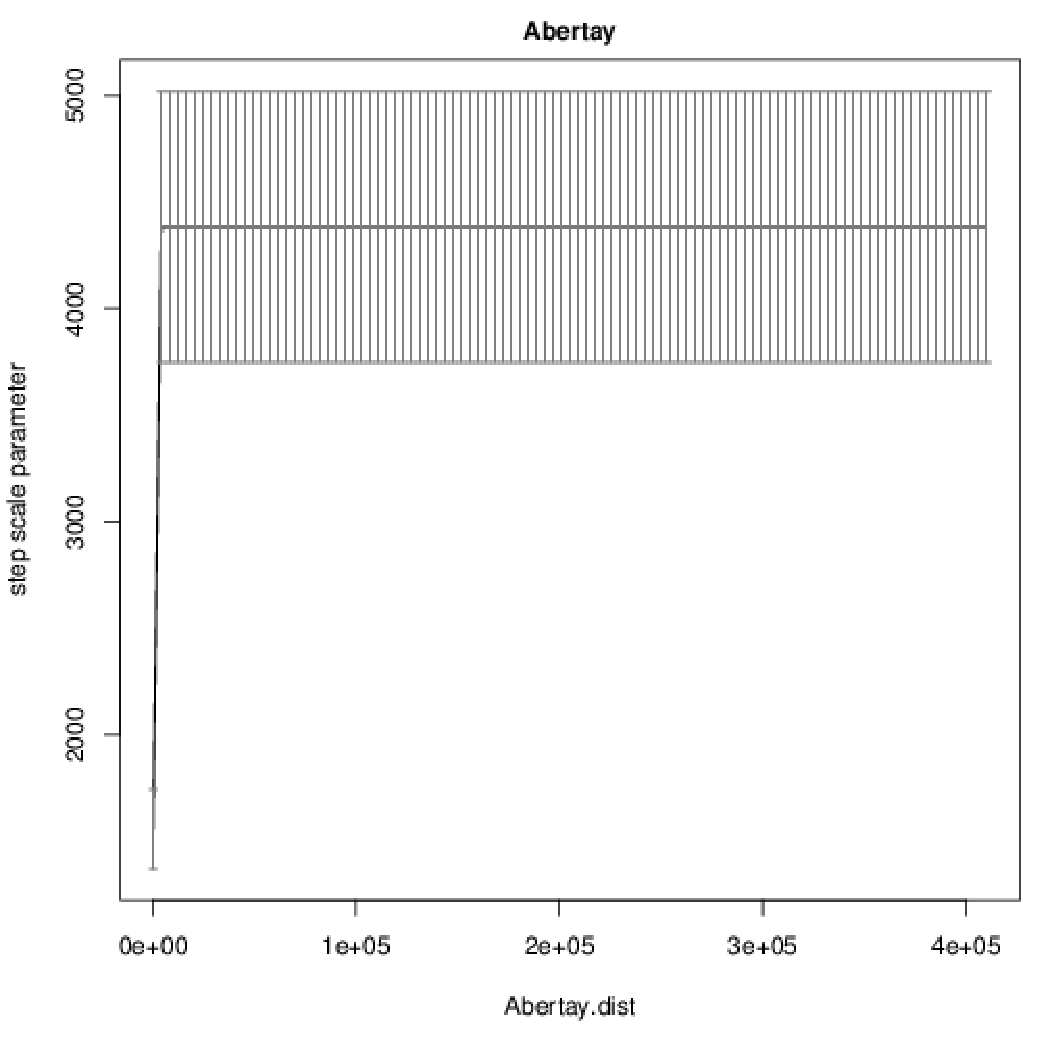
\includegraphics[width=0.49\textwidth]{plot_greySealResults002.pdf}
  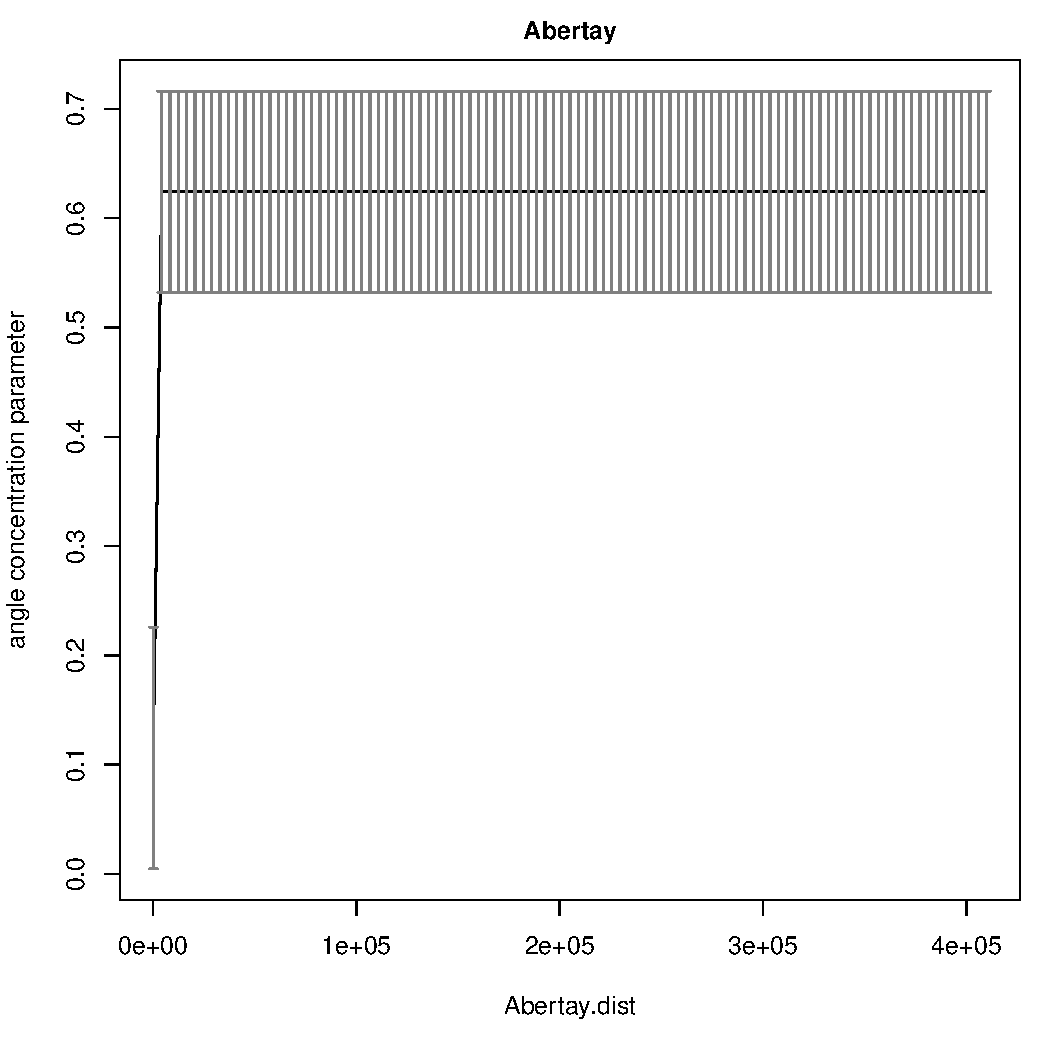
\includegraphics[width=0.49\textwidth]{plot_greySealResults009.pdf}\\
  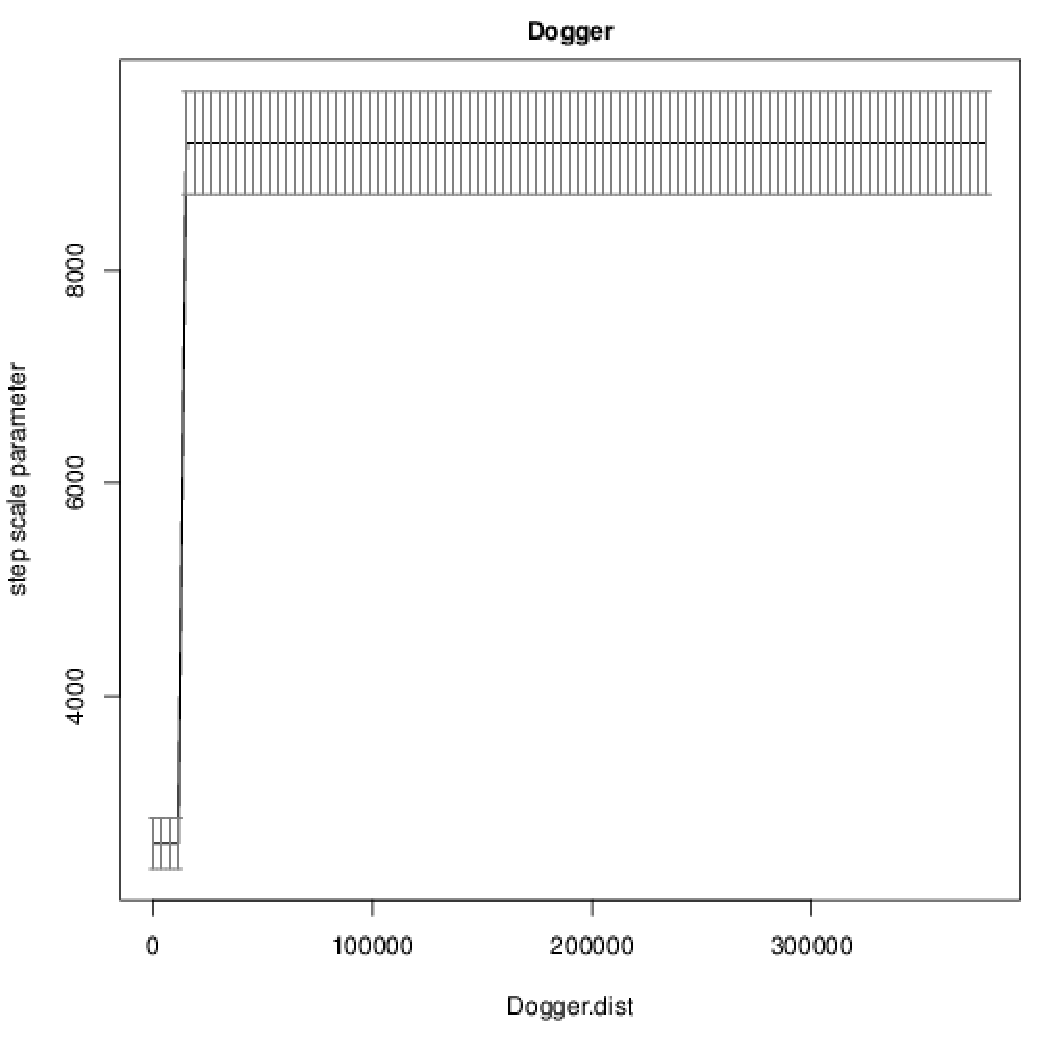
\includegraphics[width=0.49\textwidth]{plot_greySealResults006.pdf}
  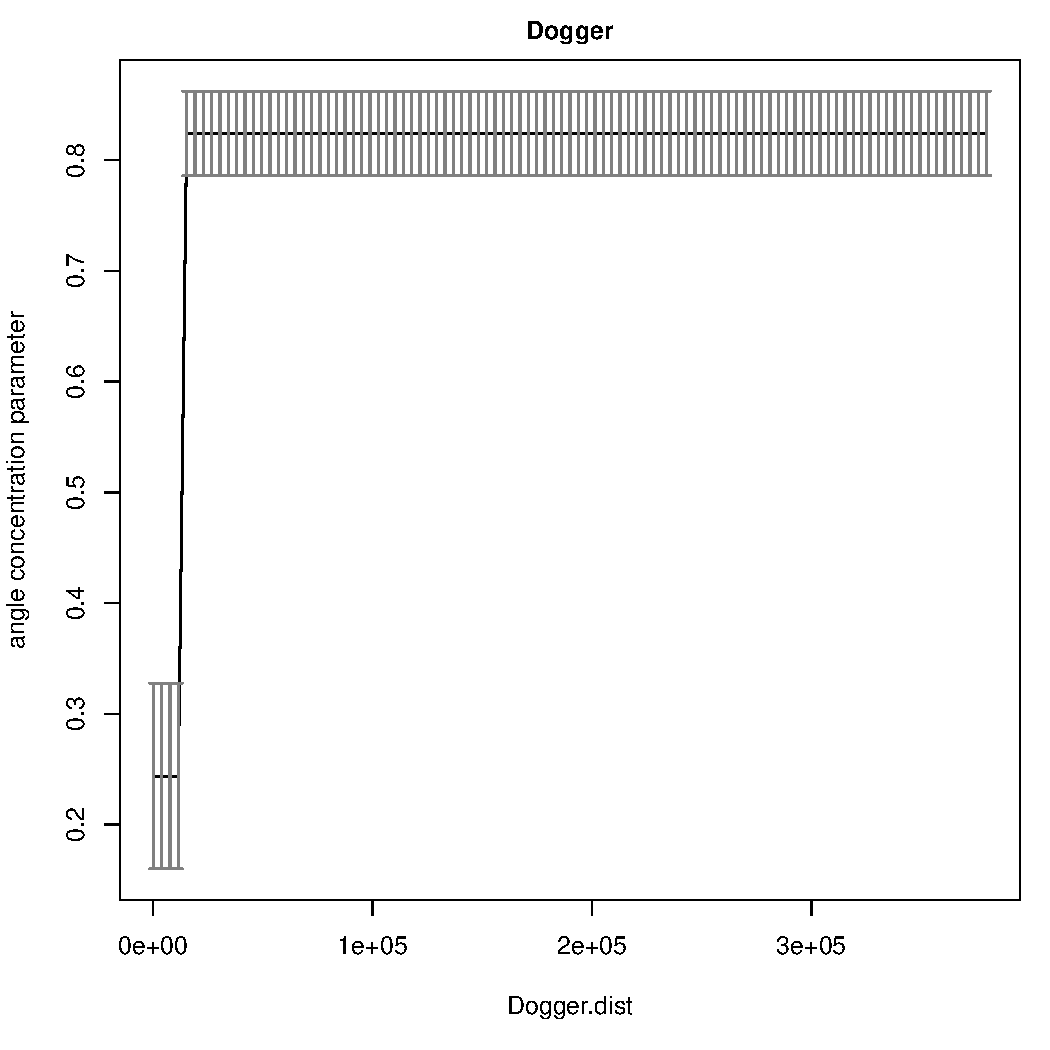
\includegraphics[width=0.49\textwidth]{plot_greySealResults013.pdf}\\
  \caption{Selected results from the grey seal example. Panels include estimates and 95\% confidence intervals for the ``Abertay'' haul-out state step length scale parameter as a function of distance in meters (`Abertay.dist'; top-left panel), ``Abertay'' haul-out state turning angle concentration parameter as a function of distance (top-right panel), ``Dogger Bank'' foraging state step length scale parameter as a function of distance (`Dogger.dist'; bottom-left panel), and the ``Dogger Bank'' foraging state turning angle concentration parameter as a function of distance (bottom-right panel).}
  \label{fig:greySealResults}
\end{figure}

\begin{figure}[htbp]
  \centering
  %\begin{adjustbox}{trim=0cm 0.25cm 0cm 1.5cm}
    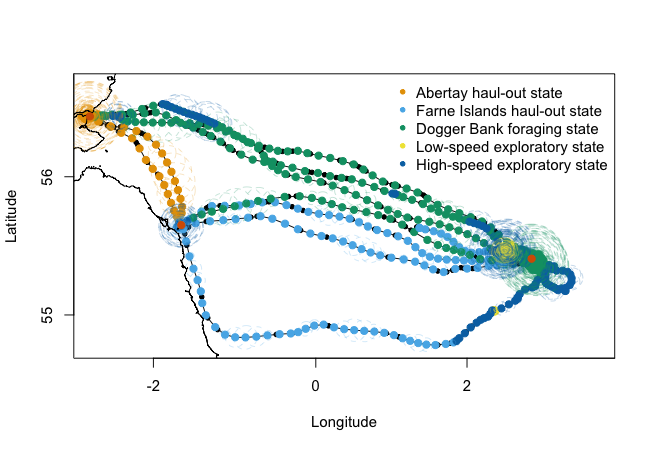
\includegraphics[width=0.8\textwidth]{plot_greySealResults1.png}\\
    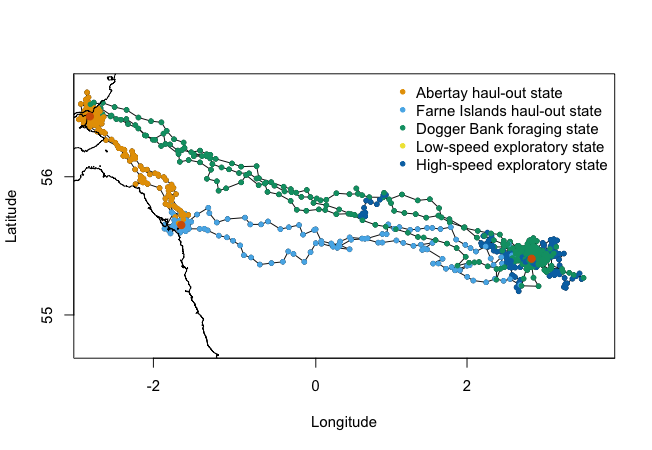
\includegraphics[width=0.8\textwidth]{plot_greySealResults2.png}
  %\end{adjustbox}
  \caption{Fitted and simulated tracks from the grey seal example. This seal tended to move in a clockwise fashion between two haul-out locations (``Abertay'' and ``Farne Islands'') and a foraging area (``Dogger Bank'') in the North Sea. Top panel plots the pooled track, 95\% error ellipse confidence bands, and state estimates based on the 5-state HMM fitted to multiple imputations of the position process. Red points indicate the locations of the three activity centers. Black points indicate the (temporally-irregular) observed locations. Bottom panel presents the locations and states for a track simulated from the fitted model using the `simData' function.}
  \label{fig:greySealStateSims}
\end{figure}

\subsection{Southern elephant seals}
\label{sec:ses}
\stoptocwriting
Here, we analyse the southern elephant seal (\emph{Mirounga leonina}) data from \cite{MichelotEtAl2017} using \verb|momentuHMM|. The data set consists of 15 tracks, each encompassing (at most) one foraging trip, starting from Kerguelen Island. We want to fit the model described by \cite{MichelotEtAl2017}, with the four following states:
\begin{enumerate}
\item outbound trip from the colony to the ice;
\item searching;
\item foraging;
\item inbound trip from the ice to the colony.
\end{enumerate}

The data set has three columns: ``ID'' (track ID), ``x'' (longitude), and ``y'' (latitude):

\begin{knitrout}
\definecolor{shadecolor}{rgb}{0.969, 0.969, 0.969}\color{fgcolor}\begin{kframe}
\begin{alltt}
\hlkwd{head}\hlstd{(tracks)}
\end{alltt}
\begin{verbatim}
##   ID        x         y
## 1  1 70.60946 -49.60737
## 2  1 70.82908 -50.08287
## 3  1 70.90029 -50.32835
## 4  1 70.85766 -50.54746
## 5  1 70.63792 -50.90529
## 6  1 70.48480 -50.99666
\end{verbatim}
\end{kframe}
\end{knitrout}

From the locations, we use \verb|prepData| to derive the step lengths and turning angles, as well as the distance and bearing (relative to previous movement direction as in Eq. \ref{eq:angleCov}) to the Kerguelen Island colony (with coordinates 70$^{\circ}$ longitude and -49$^{\circ}$ latitude):
\begin{knitrout}
\definecolor{shadecolor}{rgb}{0.969, 0.969, 0.969}\color{fgcolor}\begin{kframe}
\begin{alltt}
\hlstd{center} \hlkwb{<-} \hlkwd{matrix}\hlstd{(}\hlkwd{c}\hlstd{(}\hlnum{70}\hlstd{,}\hlopt{-}\hlnum{49}\hlstd{),}\hlkwc{nrow}\hlstd{=}\hlnum{1}\hlstd{,}\hlkwc{dimnames}\hlstd{=}\hlkwd{list}\hlstd{(}\hlstr{"colony"}\hlstd{))}
\hlstd{data} \hlkwb{<-} \hlkwd{prepData}\hlstd{(}\hlkwc{data}\hlstd{=tracks,} \hlkwc{type}\hlstd{=}\hlstr{"LL"}\hlstd{,} \hlkwc{centers}\hlstd{=center)}
\end{alltt}
\end{kframe}
\end{knitrout}
Note that distances are in kilometers and angles are based on initial bearings \citep[using geosphere::bearing;][]{Hijmans2016geo} when calculated from longitude and latitude coordinates.  

\subsubsection{Model 1: no covariates}
We start by fitting a covariate-free 4-state correlated random walk model, which we will use to extract starting parameter values for more complex models. We use the argument \verb|fixPar| to fix some transition probabilities to zero, following \cite{MichelotEtAl2017}.  We set to \verb|NA| the columns of unconstrained transition probabilities, and we fix the intercept of the other columns to a large negative number (here $-100$) to set the corresponding transition probabilities to be virtually zero (i.e.\ impossible transition).  As in \cite{MichelotEtAl2017}, we set transition probabilities from outbound to forage, outbound to inbound, search to outbound, forage to outbound, forage to inbound, inbound to outbound, inbound to search, and inbound to forage to be effectively zero.
\begin{knitrout}
\definecolor{shadecolor}{rgb}{0.969, 0.969, 0.969}\color{fgcolor}\begin{kframe}
\begin{alltt}
\hlstd{stateNames} \hlkwb{<-} \hlkwd{c}\hlstd{(}\hlstr{"outbound"}\hlstd{,}\hlstr{"search"}\hlstd{,}\hlstr{"forage"}\hlstd{,}\hlstr{"inbound"}\hlstd{)}

\hlcom{# initial parameters}
\hlstd{stepPar0} \hlkwb{<-} \hlkwd{c}\hlstd{(}\hlnum{25}\hlstd{,}\hlnum{5}\hlstd{,}\hlnum{1}\hlstd{,}\hlnum{25}\hlstd{,}\hlnum{10}\hlstd{,}\hlnum{5}\hlstd{,}\hlnum{3}\hlstd{,}\hlnum{10}\hlstd{)}
\hlstd{anglePar0} \hlkwb{<-} \hlkwd{c}\hlstd{(}\hlnum{15}\hlstd{,}\hlnum{5}\hlstd{,}\hlnum{2}\hlstd{,}\hlnum{15}\hlstd{)}

\hlcom{# constrain transition probabilities}
\hlstd{fixbeta} \hlkwb{<-} \hlkwd{matrix}\hlstd{(}\hlkwd{c}\hlstd{(}\hlnum{NA}\hlstd{,}\hlopt{-}\hlnum{100}\hlstd{,}\hlopt{-}\hlnum{100}\hlstd{,}\hlopt{-}\hlnum{100}\hlstd{,}\hlnum{NA}\hlstd{,}\hlnum{NA}\hlstd{,}\hlopt{-}\hlnum{100}\hlstd{,}\hlnum{NA}\hlstd{,}\hlopt{-}\hlnum{100}\hlstd{,}\hlopt{-}\hlnum{100}\hlstd{,}\hlopt{-}\hlnum{100}\hlstd{,}\hlopt{-}\hlnum{100}\hlstd{),}
                  \hlkwc{nrow}\hlstd{=}\hlnum{1}\hlstd{)}

\hlstd{m1} \hlkwb{<-} \hlkwd{fitHMM}\hlstd{(}\hlkwc{data}\hlstd{=data,} \hlkwc{nbStates}\hlstd{=}\hlnum{4}\hlstd{,} \hlkwc{dist}\hlstd{=}\hlkwd{list}\hlstd{(}\hlkwc{step}\hlstd{=}\hlstr{"gamma"}\hlstd{,}\hlkwc{angle}\hlstd{=}\hlstr{"vm"}\hlstd{),}
             \hlkwc{Par0}\hlstd{=}\hlkwd{list}\hlstd{(}\hlkwc{step}\hlstd{=stepPar0,} \hlkwc{angle}\hlstd{=anglePar0),}
             \hlkwc{fixPar}\hlstd{=}\hlkwd{list}\hlstd{(}\hlkwc{beta}\hlstd{=fixbeta),} \hlkwc{stateNames} \hlstd{= stateNames)}
\end{alltt}
\end{kframe}
\end{knitrout}

\subsubsection{Model 2}
\label{sec:ses2}
This model mimics the formulation of \cite{MichelotEtAl2017}. We model the effect of the distance to colony on the transition probability from outbound to search, and of the time since departure on the transition probability from search to inbound.
\begin{knitrout}
\definecolor{shadecolor}{rgb}{0.969, 0.969, 0.969}\color{fgcolor}\begin{kframe}
\begin{alltt}
\hlcom{# time spent since left colony}
\hlstd{time} \hlkwb{<-} \hlkwa{NULL}
\hlkwa{for}\hlstd{(id} \hlkwa{in} \hlkwd{unique}\hlstd{(data}\hlopt{$}\hlstd{ID)) \{}
    \hlstd{nbSubObs} \hlkwb{<-} \hlkwd{length}\hlstd{(}\hlkwd{which}\hlstd{(data}\hlopt{$}\hlstd{ID}\hlopt{==}\hlstd{id))}

    \hlcom{# approximately in months for interval = 9.6h}
    \hlstd{time} \hlkwb{<-} \hlkwd{c}\hlstd{(time, (}\hlnum{1}\hlopt{:}\hlstd{nbSubObs)}\hlopt{/}\hlnum{75}\hlstd{)}
\hlstd{\}}

\hlstd{data}\hlopt{$}\hlstd{time} \hlkwb{<-} \hlstd{time}

\hlcom{# compute time since departure and include in formula below}
\hlstd{formula} \hlkwb{<-} \hlopt{~} \hlstd{colony.dist} \hlopt{+} \hlstd{time}
\end{alltt}
\end{kframe}
\end{knitrout}

As before, we constrain the transition probability matrix to prevent some of the transitions (e.g.\ from forage to inbound, etc.). We define a $3 \times 12$ matrix for the beta parameters, in which each column corresponds to a transition ($1 \rightarrow 2, 1 \rightarrow 3, 1 \rightarrow 4, 2 \rightarrow 1, \dots$), and each row corresponds to a covariate (intercept, distance to center, time since departure). We set to \verb|NA| the columns of unconstrained transition probabilities, and we again fix the intercept of the other columns to a large negative number (here $-100$) to set the corresponding transition probabilities to be virtually zero (i.e.\ impossible transition).

\begin{knitrout}
\definecolor{shadecolor}{rgb}{0.969, 0.969, 0.969}\color{fgcolor}\begin{kframe}
\begin{alltt}
\hlstd{fixbeta} \hlkwb{<-} \hlkwd{matrix}\hlstd{(}\hlkwd{c}\hlstd{(}\hlnum{NA}\hlstd{,}\hlopt{-}\hlnum{100}\hlstd{,}\hlopt{-}\hlnum{100}\hlstd{,}\hlopt{-}\hlnum{100}\hlstd{,}\hlnum{NA}\hlstd{,}\hlnum{NA}\hlstd{,}\hlopt{-}\hlnum{100}\hlstd{,}\hlnum{NA}\hlstd{,}\hlopt{-}\hlnum{100}\hlstd{,}\hlopt{-}\hlnum{100}\hlstd{,}\hlopt{-}\hlnum{100}\hlstd{,}\hlopt{-}\hlnum{100}\hlstd{,}
                    \hlnum{NA}\hlstd{,}   \hlnum{0}\hlstd{,}   \hlnum{0}\hlstd{,}   \hlnum{0}\hlstd{,} \hlnum{0}\hlstd{,} \hlnum{0}\hlstd{,}   \hlnum{0}\hlstd{,} \hlnum{0}\hlstd{,}   \hlnum{0}\hlstd{,}   \hlnum{0}\hlstd{,}   \hlnum{0}\hlstd{,}   \hlnum{0}\hlstd{,}
                     \hlnum{0}\hlstd{,}   \hlnum{0}\hlstd{,}   \hlnum{0}\hlstd{,}   \hlnum{0}\hlstd{,} \hlnum{0}\hlstd{,}\hlnum{NA}\hlstd{,}   \hlnum{0}\hlstd{,} \hlnum{0}\hlstd{,}   \hlnum{0}\hlstd{,}   \hlnum{0}\hlstd{,}   \hlnum{0}\hlstd{,}   \hlnum{0}\hlstd{),}
                  \hlkwc{nrow}\hlstd{=}\hlnum{3}\hlstd{,}\hlkwc{byrow}\hlstd{=}\hlnum{TRUE}\hlstd{)}
\end{alltt}
\end{kframe}
\end{knitrout}

Biased random walks are used to model the movement in states 1 and 4, with repulsion away from the colony in the outbound trip, and attraction towards the colony in the inbound trip. For that purpose, we include `colony.angle' as a covariate on the angle mean of the von Mises distributions for turning angles in states 1 and 4. 

\begin{knitrout}
\definecolor{shadecolor}{rgb}{0.969, 0.969, 0.969}\color{fgcolor}\begin{kframe}
\begin{alltt}
\hlstd{angleFormula} \hlkwb{<-} \hlopt{~} \hlkwd{state1}\hlstd{(colony.angle)} \hlopt{+} \hlkwd{state4}\hlstd{(colony.angle)}
\end{alltt}
\end{kframe}
\end{knitrout}

To specify the direction of the bias (away from or towards the colony), we fix the parameters linking the mean turning angle to the direction of the colony. Because we will remove the correlated random walk component of Eq. \ref{eq:circ} for states 1 and 4 (by setting \verb|circularAngleMean=list(angle=0)|; see section \ref{sec:circ}), we fix the coefficient to $-1$ for state 1 (so that the mean direction is away from the colony), and we fix the coefficient to $+1$ for state 4 (so that the mean direction is towards the colony). Note that with only a single angular covariate, the magnitude of these fixed coefficients is not important; only the sign is important (i.e. positive for attraction, negative for repulsion). The four other parameters correspond to the angle concentrations and should be estimated (NAs in \verb|fixPar|).
\begin{knitrout}
\definecolor{shadecolor}{rgb}{0.969, 0.969, 0.969}\color{fgcolor}\begin{kframe}
\begin{alltt}
\hlstd{fixPar} \hlkwb{<-} \hlkwd{list}\hlstd{(}\hlkwc{angle}\hlstd{=}\hlkwd{c}\hlstd{(}\hlopt{-}\hlnum{1}\hlstd{,}\hlnum{1}\hlstd{,}\hlnum{NA}\hlstd{,}\hlnum{NA}\hlstd{,}\hlnum{NA}\hlstd{,}\hlnum{NA}\hlstd{),}\hlkwc{beta}\hlstd{=fixbeta)}
\end{alltt}
\end{kframe}
\end{knitrout}
Because no covariates are specified for the mean angle of state 2 (searching) and state 3 (foraging), these states are reduced to correlated random walks with a mean turning angle of zero (i.e. $\text{atan2}(0,0)=0$; see Eq. \ref{eq:circ}).

We can now fit the second model with starting parameter values extracted from the simpler model using \verb|getPar0|. In \verb|fitHMM|, we use the arguments \verb|estAngleMean| and \verb|circularAngleMean| to indicate that the angle mean is to be estimated using circular-circular regression (with short-term directional persistence removed for states 1 and 4).

\begin{knitrout}
\definecolor{shadecolor}{rgb}{0.969, 0.969, 0.969}\color{fgcolor}\begin{kframe}
\begin{alltt}
\hlstd{Par0} \hlkwb{<-} \hlkwd{getPar0}\hlstd{(}\hlkwc{model}\hlstd{=m1,} \hlkwc{nbStates}\hlstd{=}\hlnum{4}\hlstd{,}
                \hlkwc{DM}\hlstd{=}\hlkwd{list}\hlstd{(}\hlkwc{angle}\hlstd{=}\hlkwd{list}\hlstd{(}\hlkwc{mean}\hlstd{=angleFormula,} \hlkwc{concentration}\hlstd{=}\hlopt{~}\hlnum{1}\hlstd{)),}
                \hlkwc{estAngleMean}\hlstd{=}\hlkwd{list}\hlstd{(}\hlkwc{angle}\hlstd{=}\hlnum{TRUE}\hlstd{),}
                \hlkwc{circularAngleMean}\hlstd{=}\hlkwd{list}\hlstd{(}\hlkwc{angle}\hlstd{=}\hlnum{0}\hlstd{),} \hlkwc{formula}\hlstd{=formula)}

\hlstd{m2} \hlkwb{<-} \hlkwd{fitHMM}\hlstd{(}\hlkwc{data}\hlstd{=data,} \hlkwc{nbStates}\hlstd{=}\hlnum{4}\hlstd{,} \hlkwc{dist}\hlstd{=}\hlkwd{list}\hlstd{(}\hlkwc{step}\hlstd{=}\hlstr{"gamma"}\hlstd{,}\hlkwc{angle}\hlstd{=}\hlstr{"vm"}\hlstd{),}
             \hlkwc{Par0}\hlstd{=}\hlkwd{list}\hlstd{(}\hlkwc{step}\hlstd{=Par0}\hlopt{$}\hlstd{Par}\hlopt{$}\hlstd{step,} \hlkwc{angle}\hlstd{=Par0}\hlopt{$}\hlstd{Par}\hlopt{$}\hlstd{angle),}
             \hlkwc{beta0}\hlstd{=Par0}\hlopt{$}\hlstd{beta,} \hlkwc{fixPar}\hlstd{=fixPar,} \hlkwc{formula}\hlstd{=formula,}
             \hlkwc{DM}\hlstd{=}\hlkwd{list}\hlstd{(}\hlkwc{angle}\hlstd{=}\hlkwd{list}\hlstd{(}\hlkwc{mean}\hlstd{=angleFormula,} \hlkwc{concentration}\hlstd{=}\hlopt{~}\hlnum{1}\hlstd{)),}
             \hlkwc{estAngleMean}\hlstd{=}\hlkwd{list}\hlstd{(}\hlkwc{angle}\hlstd{=}\hlnum{TRUE}\hlstd{),} \hlkwc{circularAngleMean}\hlstd{=}\hlkwd{list}\hlstd{(}\hlkwc{angle}\hlstd{=}\hlnum{0}\hlstd{),}
             \hlkwc{stateNames} \hlstd{= stateNames)}
\end{alltt}
\end{kframe}
\end{knitrout}

Instead of relying entirely on \verb|fixPar| for parameter constraints, an equivalent model for the transition probabilities could be specified using the special function \verb|betaCol| in \verb|formula|:
\begin{knitrout}
\definecolor{shadecolor}{rgb}{0.969, 0.969, 0.969}\color{fgcolor}\begin{kframe}
\begin{alltt}
\hlstd{formula} \hlkwb{<-} \hlopt{~} \hlkwd{betaCol1}\hlstd{(colony.dist)} \hlopt{+} \hlkwd{betaCol6}\hlstd{(time)}

\hlstd{fixbeta} \hlkwb{<-} \hlkwd{matrix}\hlstd{(}\hlkwd{c}\hlstd{(}\hlnum{NA}\hlstd{,}\hlopt{-}\hlnum{100}\hlstd{,}\hlopt{-}\hlnum{100}\hlstd{,}\hlopt{-}\hlnum{100}\hlstd{,}\hlnum{NA}\hlstd{,}\hlnum{NA}\hlstd{,}\hlopt{-}\hlnum{100}\hlstd{,}\hlnum{NA}\hlstd{,}\hlopt{-}\hlnum{100}\hlstd{,}\hlopt{-}\hlnum{100}\hlstd{,}\hlopt{-}\hlnum{100}\hlstd{,}\hlopt{-}\hlnum{100}\hlstd{,}
                    \hlkwd{rep}\hlstd{(}\hlnum{NA}\hlstd{,}\hlnum{12}\hlstd{),}
                    \hlkwd{rep}\hlstd{(}\hlnum{NA}\hlstd{,}\hlnum{12}\hlstd{)),}
                  \hlkwc{nrow}\hlstd{=}\hlnum{3}\hlstd{,}\hlkwc{byrow}\hlstd{=}\hlnum{TRUE}\hlstd{)}

\hlstd{fixPar} \hlkwb{<-} \hlkwd{list}\hlstd{(}\hlkwc{angle}\hlstd{=}\hlkwd{c}\hlstd{(}\hlopt{-}\hlnum{1}\hlstd{,}\hlnum{1}\hlstd{,}\hlnum{NA}\hlstd{,}\hlnum{NA}\hlstd{,}\hlnum{NA}\hlstd{,}\hlnum{NA}\hlstd{),}\hlkwc{beta}\hlstd{=fixbeta)}
\end{alltt}
\end{kframe}
\end{knitrout}
Here \verb|betaCol1(colony.dist)| specifies an effect of distance to colony only on the transition from state 1 to state 2 (which corresponds to the first column of the beta matrix) and \verb|betaCol6(time)| specifies an effect of time since departure only on the transition from state 2 to state 4 (which corresponds to the sixth column of the beta matrix).  When the special function \verb|betaCol| is used, then \verb|fitHMM| automatically fixes the appropriate elements in the second (`colony.dist') and third (`time') rows of the beta matrix to zero (without the user needing to do so manually using \verb|fixPar|). However, note that the first row (corresponding to the intercept terms) must still be manually fixed to achieve the desired constraints on the transition probability matrix.

\subsubsection{Model 3}
In addition to the covariates included in model 2, we add the effect of distance to colony on the step length and turning angle concentration parameters for states 1 and 4. We specify the following formulas:
\begin{knitrout}
\definecolor{shadecolor}{rgb}{0.969, 0.969, 0.969}\color{fgcolor}\begin{kframe}
\begin{alltt}
\hlstd{distFormula} \hlkwb{<-} \hlopt{~} \hlkwd{state1}\hlstd{(colony.dist)} \hlopt{+} \hlkwd{state4}\hlstd{(colony.dist)}
\hlstd{stepDM} \hlkwb{<-} \hlkwd{list}\hlstd{(}\hlkwc{mean}\hlstd{=distFormula,} \hlkwc{sd}\hlstd{=distFormula)}
\hlstd{angleDM} \hlkwb{<-} \hlkwd{list}\hlstd{(}\hlkwc{mean}\hlstd{=angleFormula,} \hlkwc{concentration}\hlstd{=distFormula)}
\end{alltt}
\end{kframe}
\end{knitrout}

The initial parameters are extracted from model 2, again using the function \verb|getPar0|. Instead of fixing the mean direction of movement like in model 2, we estimate it here as a trade-off between short-term directional persistence and bias toward (or away) from the colony (i.e. a biased correlated random walk as in Eq. \ref{eq:circ}).
\begin{knitrout}
\definecolor{shadecolor}{rgb}{0.969, 0.969, 0.969}\color{fgcolor}\begin{kframe}
\begin{alltt}
\hlcom{# remove fixed angle parameters}
\hlstd{fixPar} \hlkwb{<-} \hlkwd{list}\hlstd{(}\hlkwc{beta}\hlstd{=fixbeta)}

\hlcom{# get starting parameters from m2}
\hlstd{Par0} \hlkwb{<-} \hlkwd{getPar0}\hlstd{(}\hlkwc{model}\hlstd{=m2,} \hlkwc{nbStates}\hlstd{=}\hlnum{4}\hlstd{,}
                \hlkwc{DM} \hlstd{=} \hlkwd{list}\hlstd{(}\hlkwc{step}\hlstd{=stepDM,} \hlkwc{angle}\hlstd{=angleDM),}
                \hlkwc{estAngleMean}\hlstd{=}\hlkwd{list}\hlstd{(}\hlkwc{angle}\hlstd{=}\hlnum{TRUE}\hlstd{),}
                \hlkwc{circularAngleMean}\hlstd{=}\hlkwd{list}\hlstd{(}\hlkwc{angle}\hlstd{=}\hlnum{TRUE}\hlstd{),}
                \hlkwc{formula}\hlstd{=formula)}

\hlcom{# the bias is estimated rather than fixed}
\hlstd{Par0}\hlopt{$}\hlstd{Par}\hlopt{$}\hlstd{angle[}\hlkwd{c}\hlstd{(}\hlstr{"mean_1:(colony.angle)"}\hlstd{,}\hlstr{"mean_4:(colony.angle)"}\hlstd{)]} \hlkwb{<-} \hlnum{0}

\hlstd{m3} \hlkwb{<-} \hlkwd{fitHMM}\hlstd{(}\hlkwc{data}\hlstd{=data,} \hlkwc{nbStates}\hlstd{=}\hlnum{4}\hlstd{,} \hlkwc{dist}\hlstd{=}\hlkwd{list}\hlstd{(}\hlkwc{step}\hlstd{=}\hlstr{"gamma"}\hlstd{,}\hlkwc{angle}\hlstd{=}\hlstr{"vm"}\hlstd{),}
             \hlkwc{Par0}\hlstd{=}\hlkwd{list}\hlstd{(}\hlkwc{step}\hlstd{=Par0}\hlopt{$}\hlstd{Par}\hlopt{$}\hlstd{step,} \hlkwc{angle}\hlstd{=Par0}\hlopt{$}\hlstd{Par}\hlopt{$}\hlstd{angle),}
             \hlkwc{beta0}\hlstd{=Par0}\hlopt{$}\hlstd{beta,} \hlkwc{fixPar}\hlstd{=fixPar,} \hlkwc{formula}\hlstd{=formula,}
             \hlkwc{DM} \hlstd{=} \hlkwd{list}\hlstd{(}\hlkwc{step}\hlstd{=stepDM,} \hlkwc{angle}\hlstd{=angleDM),}
             \hlkwc{estAngleMean}\hlstd{=}\hlkwd{list}\hlstd{(}\hlkwc{angle}\hlstd{=}\hlnum{TRUE}\hlstd{),}
             \hlkwc{circularAngleMean}\hlstd{=}\hlkwd{list}\hlstd{(}\hlkwc{angle}\hlstd{=}\hlnum{TRUE}\hlstd{),}
             \hlkwc{stateNames} \hlstd{= stateNames)}
\end{alltt}
\end{kframe}
\end{knitrout}

The three fitted model can be compared with \verb|AIC(m1,m2,m3)|, which overwhelmingly supports model 3. The most likely state sequence is obtained with \verb|viterbi(m3)|. Figure \ref{fig:sesTracks} shows a map of the state-decoded track. The estimated circular-circular regression coefficients for the angle means of state 1 (outbound) and state 4 (inbound) were $-0.66$ (95\% CI: $-0.82--0.5$) and $0.4$ (95\% CI: $0.32-0.49$), respectively, thus indicating biased correlated random walks with repulsion away from the colony during outbound movements and attraction towards the colony during inbound movements. The estimated regression coefficients for the step length mean and turning angle concentration parameters for states 1 and 4 suggest that step lengths decreased and turning angles became more concentrated at the mean angle as distance to colony increased (Figure \ref{fig:sesResults})

\begin{figure}[htbp]
  \centering
  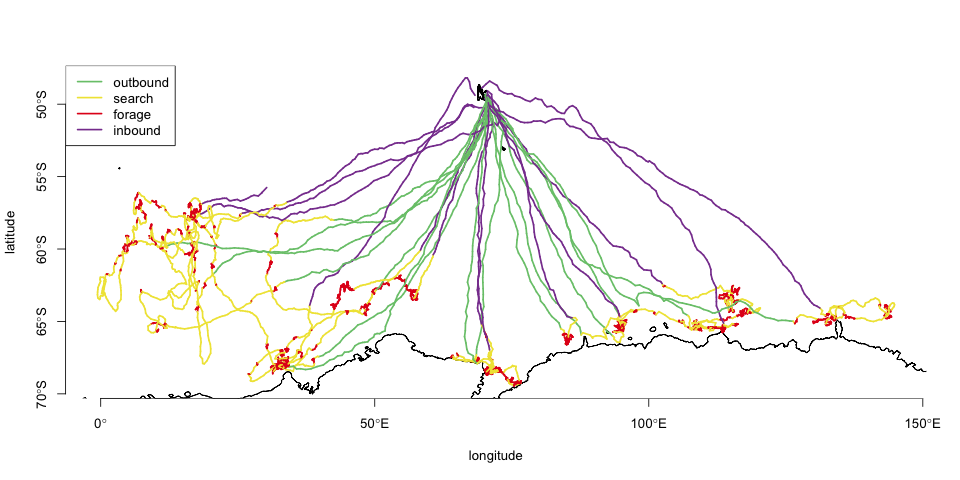
\includegraphics[width=\textwidth]{plot_sesResults2.png}
  \caption{The 15 elephant seal tracks, colored by the most likely state sequence.}
  \label{fig:sesTracks}
\end{figure}

\begin{figure}[htbp]
  \centering
  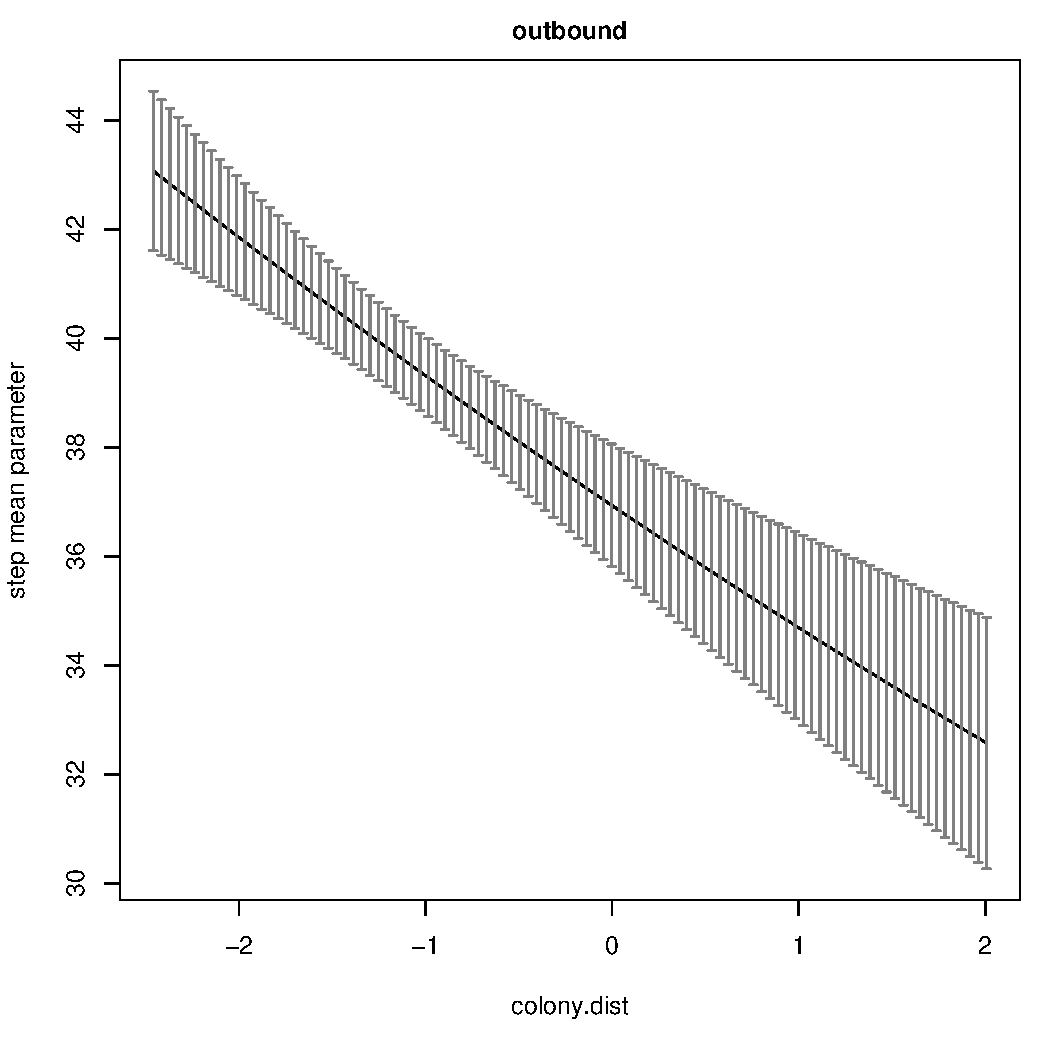
\includegraphics[width=0.49\textwidth]{plot_sesResults001.pdf}
  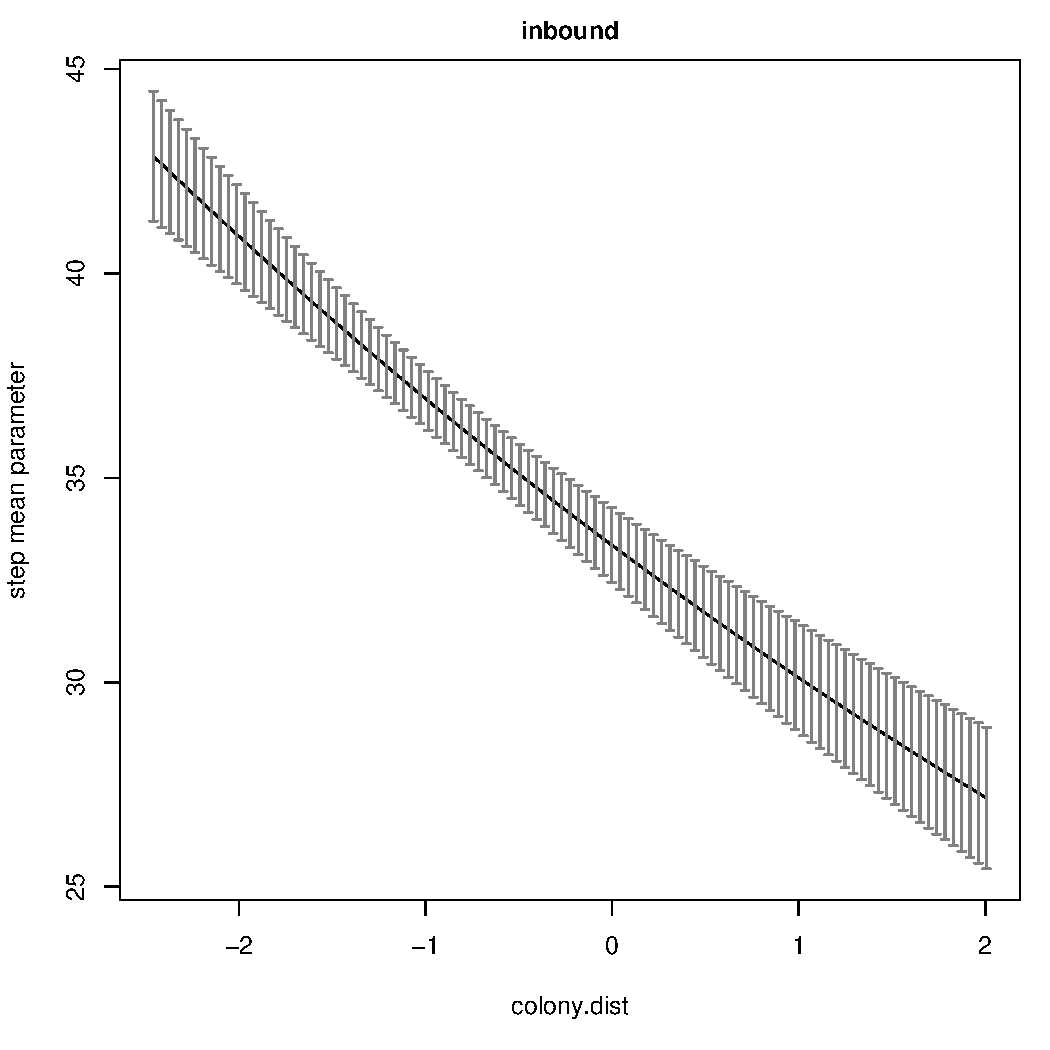
\includegraphics[width=0.49\textwidth]{plot_sesResults003.pdf}\\
  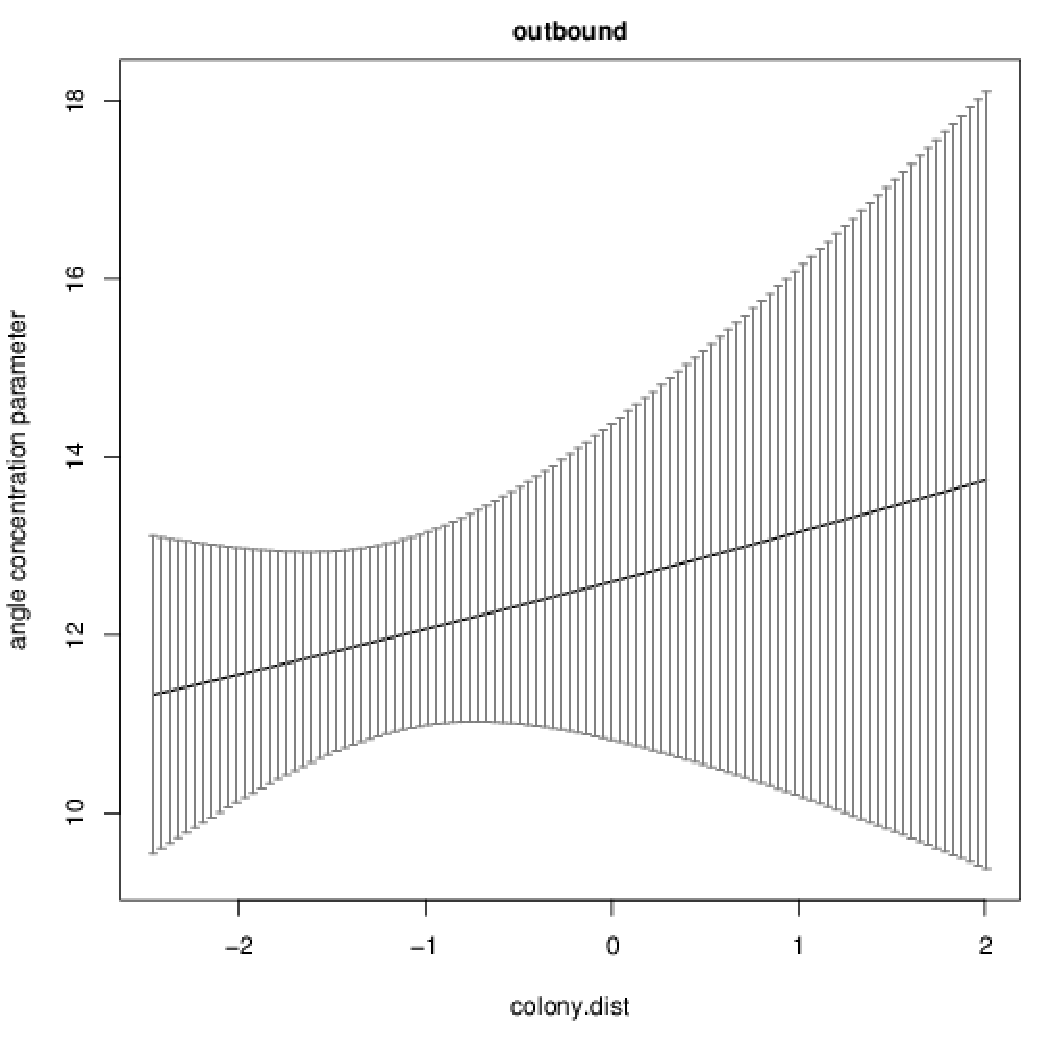
\includegraphics[width=0.49\textwidth]{plot_sesResults007.pdf}
  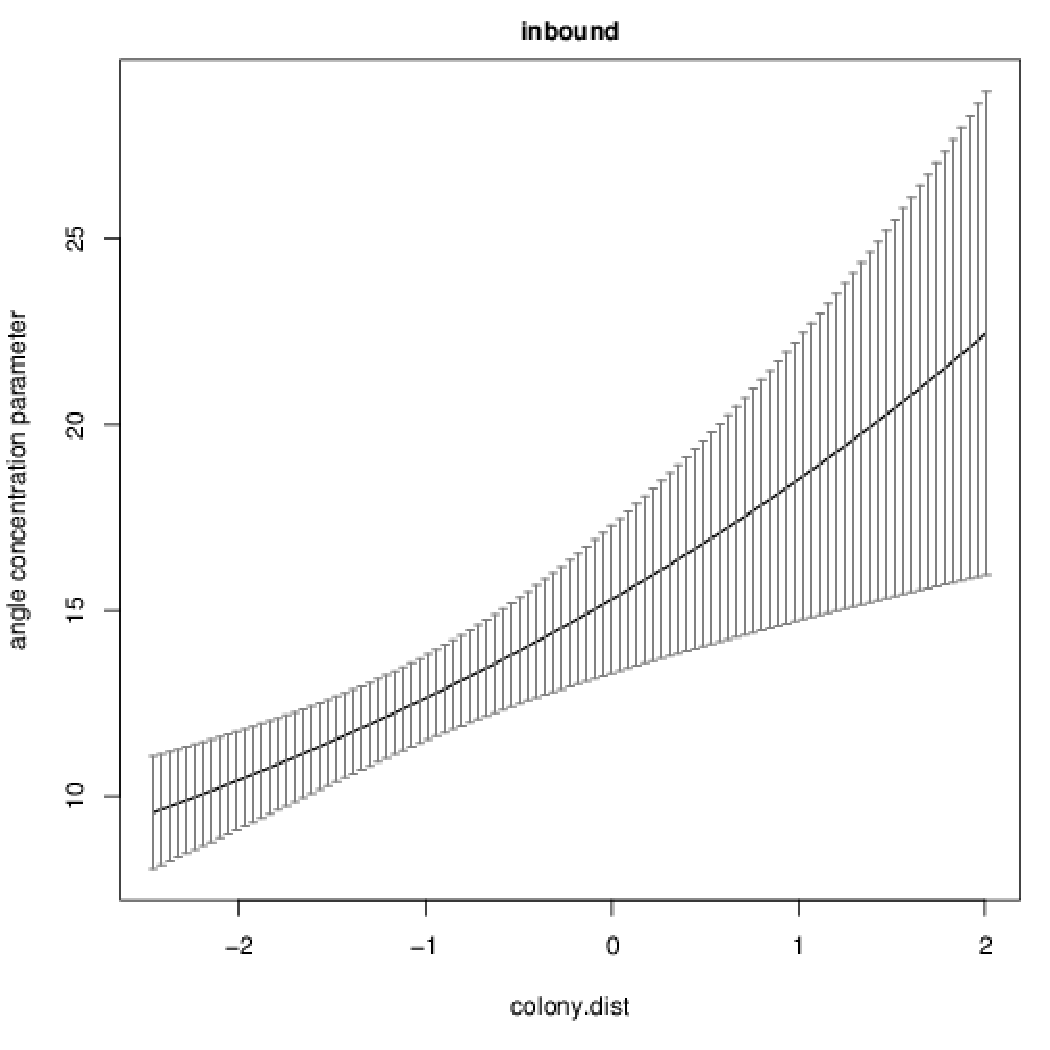
\includegraphics[width=0.49\textwidth]{plot_sesResults009.pdf}\\
  \caption{Selected results from the elephant seal example. Panels include estimates and 95\% confidence intervals for the ``outbound'' mean step length parameter (top-left panel), ``inbound'' mean step length parameter (top-right panel), ``outbound'' turning angle concentration parameter (bottom-left panel), and ``inbound'' turning angle concentration parameter (bottom-right panel) as a function of distance to colony (`colony.dist'). Distance to colony has been standardized based on a mean of 2539 km (SD = 1021.3).}
  \label{fig:sesResults}
\end{figure}
\resumetocwriting

\subsection{Group dynamic animal movement}
\label{sec:groupModel}
Here we demonstrate how \verb|momentuHMM| can be used to simulate and fit the group dynamic animal movement model of \cite{LangrockEtAl2014}. In group dynamic models, groups (e.g., herds, packs, schools) are allowed to influence the movement of social individuals. One way to accomplish this is to model individual movements as being attracted to a group ``centroid''. Depending on the system, the centroid could simply be the location of the group center (e.g., the mathematical centroid of the group) or group leader (e.g., alpha wolf) at times $t=1,\dots,T$.  In this sense, the centroid can be considered a dynamic activity center that changes position over time, and these models are not necessarily limited to groups.  For example, the centroid could instead refer to predators, competitors, or human activity (in which case the centroid might be repulsive rather than attractive!). 

Dynamic activity centers can be simulated in \verb|simData| using the \verb|centroids| argument.  Following simulation scenario A of \cite{LangrockEtAl2014}, we first simulate a group centroid as a single-state (i.e. $N=1$) biased correlated random walk relative to the origin:
\begin{knitrout}
\definecolor{shadecolor}{rgb}{0.969, 0.969, 0.969}\color{fgcolor}\begin{kframe}
\begin{alltt}
\hlstd{dist} \hlkwb{<-} \hlkwd{list}\hlstd{(}\hlkwc{step}\hlstd{=}\hlstr{"gamma"}\hlstd{,} \hlkwc{angle}\hlstd{=}\hlstr{"vm"}\hlstd{)}
\hlstd{nbObs} \hlkwb{<-} \hlnum{250}

\hlstd{Parc} \hlkwb{<-} \hlkwd{list}\hlstd{(}\hlkwc{step} \hlstd{=} \hlkwd{c}\hlstd{(}\hlnum{15}\hlstd{,}\hlnum{10}\hlstd{),}
             \hlkwc{angle} \hlstd{=} \hlkwd{c}\hlstd{(}\hlnum{0.15}\hlstd{,}\hlkwd{log}\hlstd{(}\hlnum{1}\hlstd{)))}

\hlstd{DMc} \hlkwb{<-} \hlkwd{list}\hlstd{(}\hlkwc{angle}\hlstd{=}\hlkwd{list}\hlstd{(}\hlkwc{mean} \hlstd{=} \hlopt{~}\hlstd{center1.angle,}
                       \hlkwc{concentration}\hlstd{=}\hlopt{~}\hlnum{1}\hlstd{))}

\hlstd{centroidData} \hlkwb{<-} \hlkwd{simData}\hlstd{(}\hlkwc{nbStates}\hlstd{=}\hlnum{1}\hlstd{,} \hlkwc{dist}\hlstd{=dist,} \hlkwc{Par}\hlstd{=Parc,} \hlkwc{DM}\hlstd{=DMc,}
                        \hlkwc{circularAngleMean} \hlstd{=} \hlkwd{list}\hlstd{(}\hlkwc{angle} \hlstd{=} \hlnum{TRUE}\hlstd{),}
                        \hlkwc{centers} \hlstd{=} \hlkwd{matrix}\hlstd{(}\hlnum{0}\hlstd{,}\hlnum{1}\hlstd{,}\hlnum{2}\hlstd{),}
                        \hlkwc{obsPerAnimal} \hlstd{= nbObs)}
\end{alltt}
\end{kframe}
\end{knitrout}
\begin{figure}[htbp]
  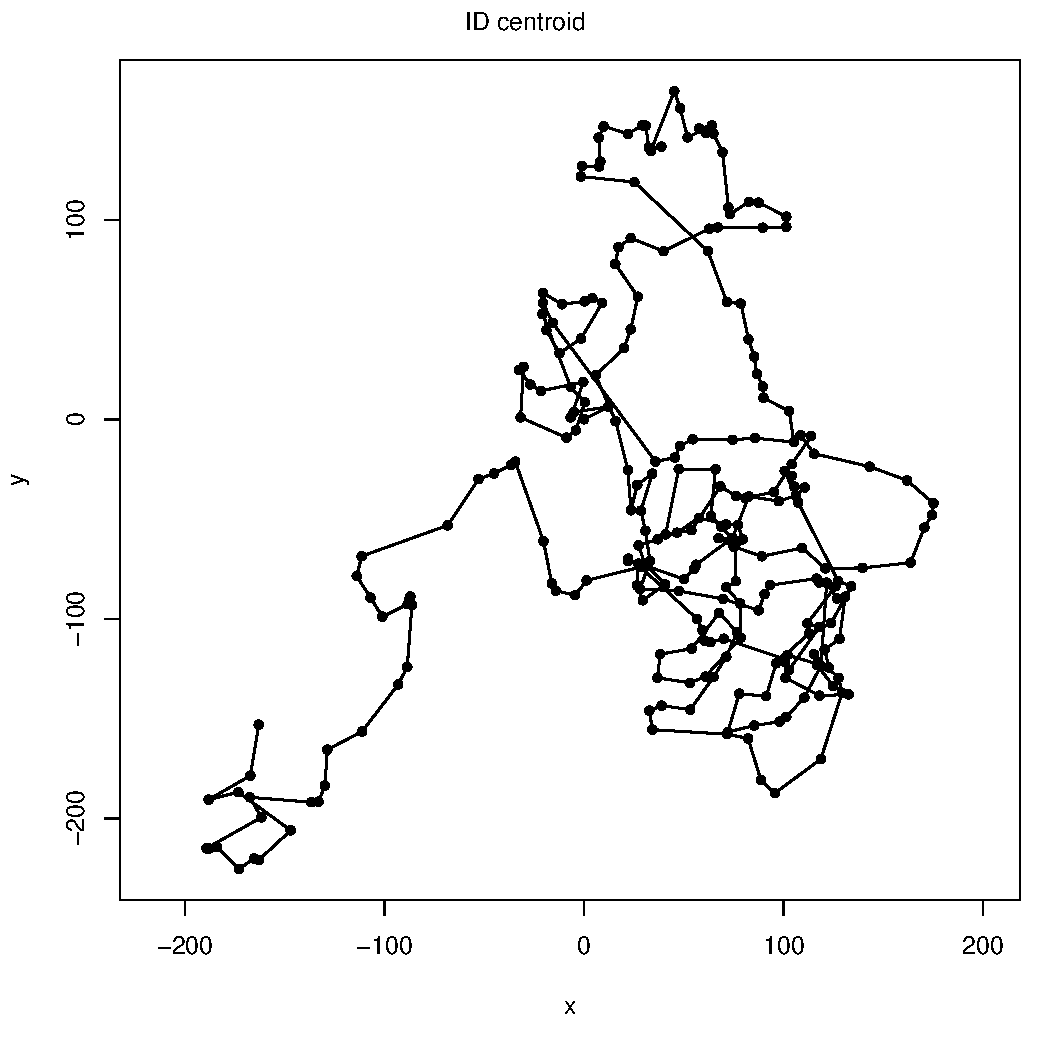
\includegraphics[width=0.49\textwidth]{plot_groupExampleCentroid001.pdf}
  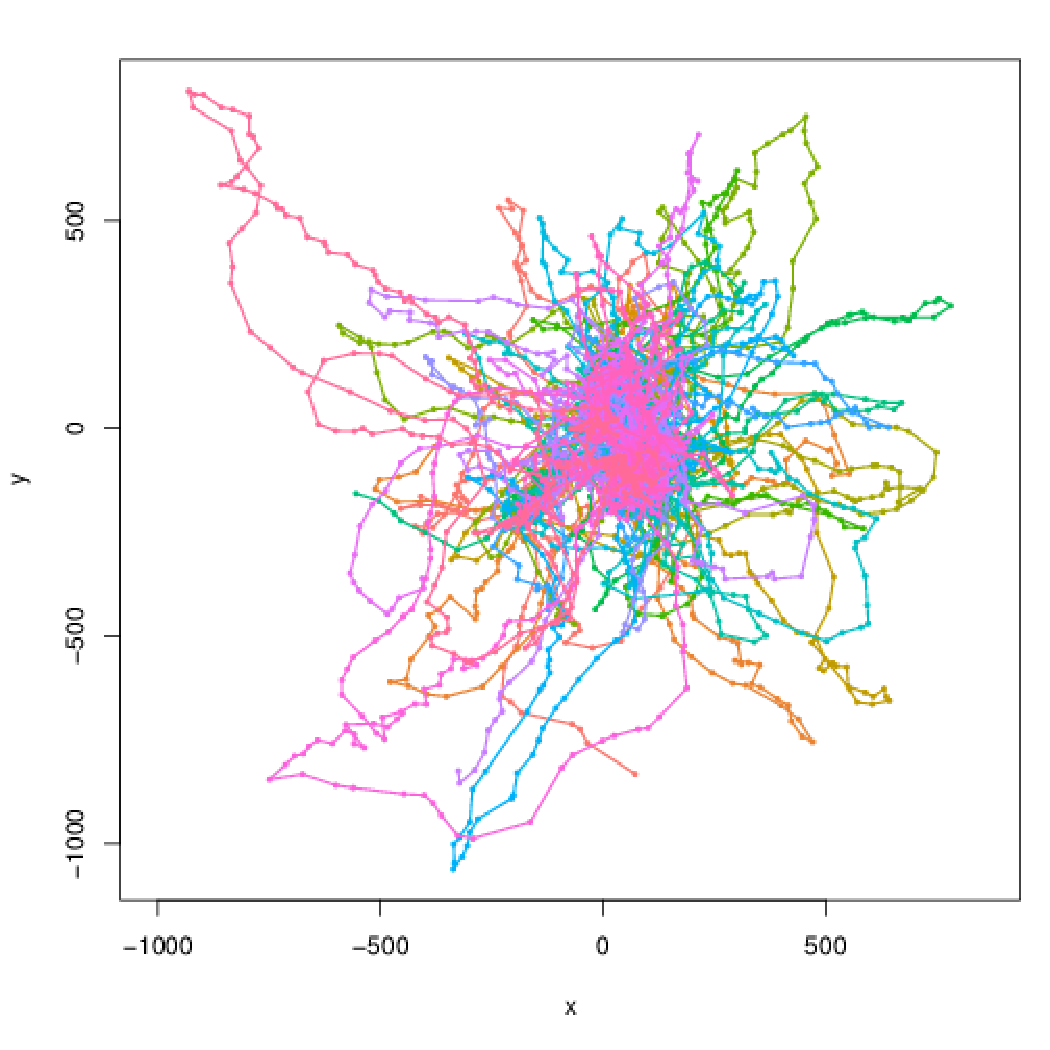
\includegraphics[width=0.49\textwidth]{plot_groupExample001.pdf}\\
  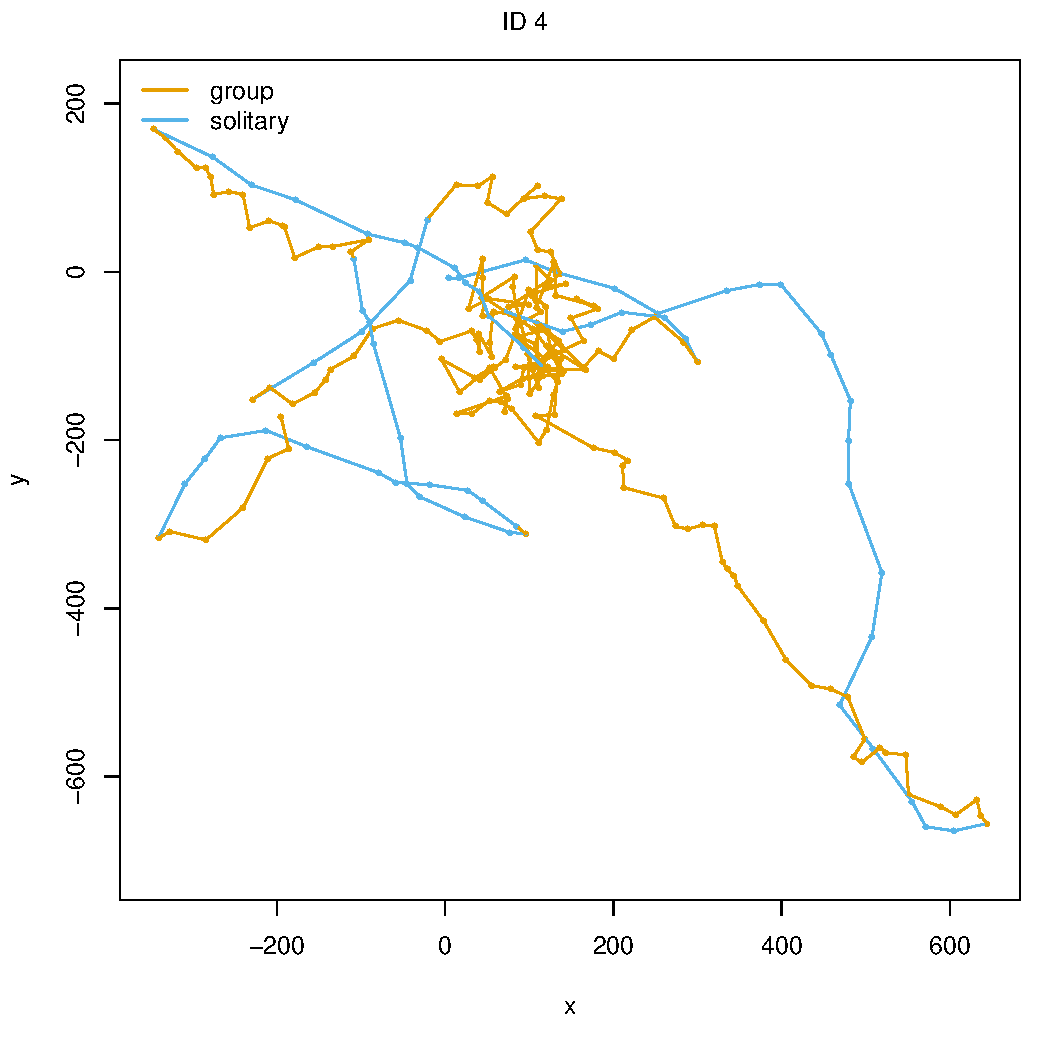
\includegraphics[width=0.49\textwidth]{plot_groupExampleResults007.pdf}
  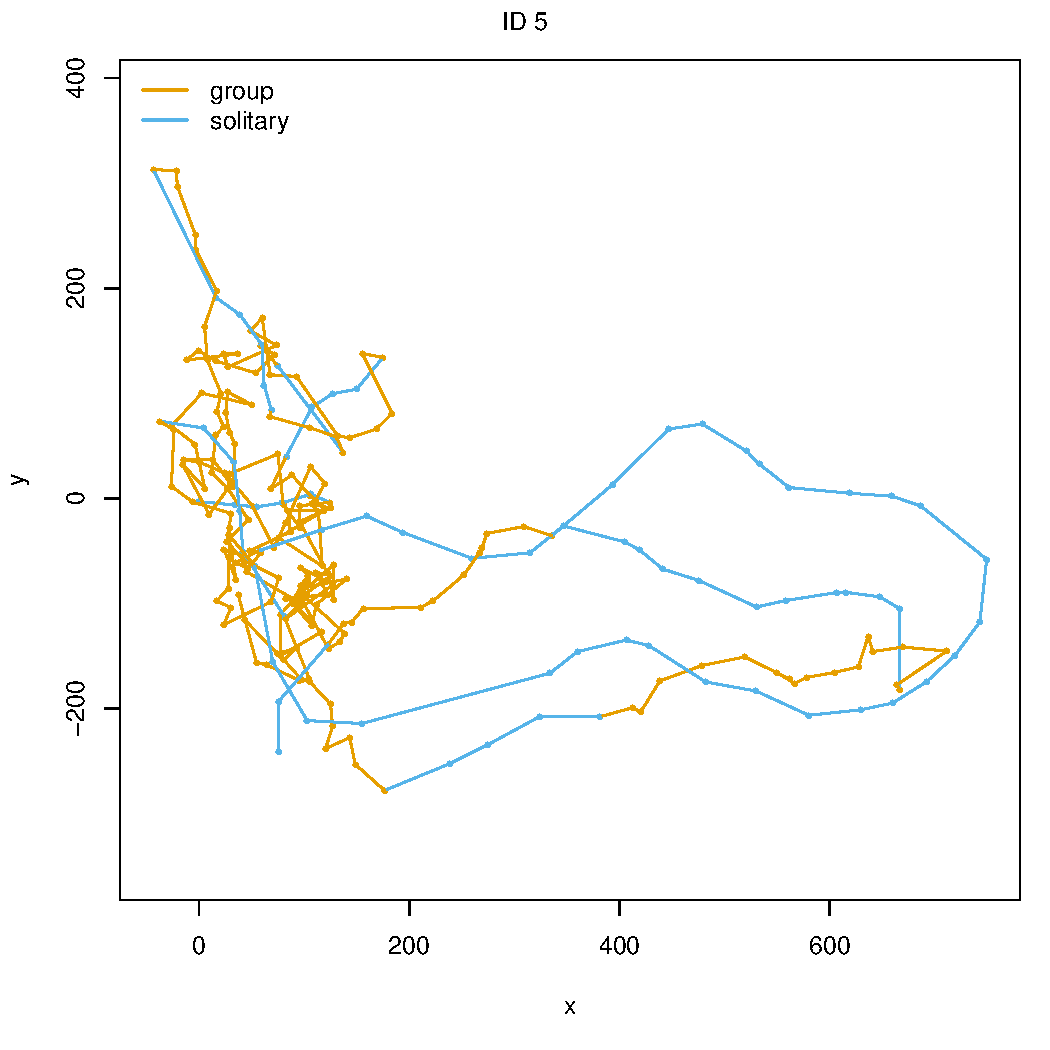
\includegraphics[width=0.49\textwidth]{plot_groupExampleResults008.pdf}\\
  \caption{Selected results from the group dynamic animal movement example. Panels include the simulated centroid path (top-left panel), the simulated paths of 20 individuals where state 1 (``group'') includes biased movements towards the centroid and state 2 (``solitary'') is a correlated random walk independent of the group centroid (top-right panel), and two fitted tracks that are colored by the most likely state sequence (bottom panels).}
  \label{fig:groupResults}
\end{figure}
Now we can use the simulated centroid track (Fig. \ref{fig:groupResults}) as a dynamic activity center and simulate the movement of a group of 20 individuals as a 2-state mixture of a biased random walk (relative to the centroid) and a correlated random walk (independent of the centroid):
\begin{knitrout}
\definecolor{shadecolor}{rgb}{0.969, 0.969, 0.969}\color{fgcolor}\begin{kframe}
\begin{alltt}
\hlstd{nbAnimals} \hlkwb{<-} \hlnum{20}
\hlstd{nbStates} \hlkwb{<-} \hlnum{2}
\hlstd{stateNames} \hlkwb{<-} \hlkwd{c}\hlstd{(}\hlstr{"group"}\hlstd{,}\hlstr{"solitary"}\hlstd{)}

\hlstd{Par} \hlkwb{<-} \hlkwd{list}\hlstd{(}\hlkwc{step} \hlstd{=} \hlkwd{c}\hlstd{(}\hlnum{30}\hlstd{,}\hlnum{50}\hlstd{,}\hlnum{15}\hlstd{,}\hlnum{25}\hlstd{),}
            \hlkwc{angle} \hlstd{=} \hlkwd{c}\hlstd{(}\hlnum{1}\hlstd{,}\hlkwd{log}\hlstd{(}\hlnum{2.5}\hlstd{),}\hlkwd{log}\hlstd{(}\hlnum{5}\hlstd{)))}

\hlstd{beta} \hlkwb{<-} \hlkwd{matrix}\hlstd{(}\hlkwd{c}\hlstd{(}\hlopt{-}\hlnum{2.944439}\hlstd{,}\hlopt{-}\hlnum{1.734601}\hlstd{),}\hlnum{1}\hlstd{,nbStates)}

\hlstd{DM} \hlkwb{<-} \hlkwd{list}\hlstd{(}\hlkwc{angle}\hlstd{=}\hlkwd{list}\hlstd{(}\hlkwc{mean} \hlstd{=} \hlopt{~}\hlkwd{state1}\hlstd{(centroid.angle),}
                      \hlkwc{concentration} \hlstd{=} \hlopt{~}\hlnum{1}\hlstd{))}

\hlcom{# calculate stationary distribution}
\hlstd{gamma} \hlkwb{<-} \hlkwd{diag}\hlstd{(nbStates)}
\hlstd{gamma[}\hlopt{!}\hlstd{gamma]} \hlkwb{<-} \hlkwd{exp}\hlstd{(beta)}
\hlstd{gamma} \hlkwb{<-} \hlkwd{t}\hlstd{(gamma)}
\hlstd{gamma} \hlkwb{<-} \hlstd{gamma}\hlopt{/}\hlkwd{apply}\hlstd{(gamma,}\hlnum{1}\hlstd{,sum)}
\hlstd{delta} \hlkwb{<-} \hlkwd{solve}\hlstd{(}\hlkwd{diag}\hlstd{(nbStates)} \hlopt{-} \hlkwd{t}\hlstd{(gamma)} \hlopt{+} \hlnum{1}\hlstd{,} \hlkwd{rep}\hlstd{(}\hlnum{1}\hlstd{, nbStates))}

\hlcom{# draw random initial locations for each individual}
\hlstd{initialPositions} \hlkwb{<-} \hlkwd{vector}\hlstd{(}\hlstr{"list"}\hlstd{)}
\hlkwa{for} \hlstd{(i} \hlkwa{in} \hlnum{1}\hlopt{:}\hlstd{nbAnimals) \{}
  \hlstd{initialPositions[[i]]} \hlkwb{<-} \hlkwd{runif}\hlstd{(}\hlnum{2}\hlstd{,} \hlopt{-}\hlnum{10}\hlstd{,} \hlnum{10}\hlstd{)}
\hlstd{\}}

\hlcom{# create centroid data frame}
\hlstd{cD} \hlkwb{<-} \hlkwd{data.frame}\hlstd{(}\hlkwc{x} \hlstd{= centroidData}\hlopt{$}\hlstd{x,} \hlkwc{y} \hlstd{= centroidData}\hlopt{$}\hlstd{y)}

\hlstd{groupData} \hlkwb{<-} \hlkwd{simData}\hlstd{(}\hlkwc{nbAnimals}\hlstd{=nbAnimals,} \hlkwc{nbStates}\hlstd{=nbStates,} \hlkwc{dist}\hlstd{=dist,}
                     \hlkwc{Par} \hlstd{= Par,} \hlkwc{beta} \hlstd{= beta,} \hlkwc{delta} \hlstd{= delta,} \hlkwc{DM} \hlstd{= DM,}
                     \hlkwc{circularAngleMean} \hlstd{=} \hlkwd{list}\hlstd{(}\hlkwc{angle} \hlstd{=} \hlnum{0}\hlstd{),}
                     \hlkwc{centroids} \hlstd{=} \hlkwd{list}\hlstd{(}\hlkwc{centroid} \hlstd{= cD),}
                     \hlkwc{obsPerAnimal} \hlstd{= nbObs,}
                     \hlkwc{initialPosition} \hlstd{= initialPositions,}
                     \hlkwc{states} \hlstd{=} \hlnum{TRUE}\hlstd{,} \hlkwc{stateNames} \hlstd{= stateNames)}
\end{alltt}
\end{kframe}
\end{knitrout}
\noindent Here state 1 (``group'') has biased movements toward the centroid and state 2 (``solitary'') is simply a correlated random walk independent of the group centroid (Fig. \ref{fig:groupResults}).  Note that despite this being a 2-state HMM, the working scale parameters for turning angle (\verb|Par$angle|) only includes 3 parameters (1 for the angle mean and 2 for the concentration parameters).  This is because under the circular-circular regression model, no working parameter is specified\footnote{More accurately, the working parameter for the reference angle is automatically fixed to $\beta_0=1$ (or whatever scalar is provided by the circularAngleMean argument).} for the reference turning angle of zero (i.e., the component for short-term directional persistence; see Eq. \ref{eq:circ}) and no angular covariates were specified in the model for state 2 (``solitary''). Thus the first parameter corresponds to the working scale parameter of the \verb|centroid.angle| covariate for state 1 (``group''), while the second and third parameters are the working scale parameters for the concentration parameters for states 1 and 2, respectively.  In this case, we remove the correlated random walk component for state 1 by setting \verb|circularAngleMean = list(angle = 0)|, and the angle mean parameter for state 1 was set at a positive value $(+1)$ to enforce a biased random walk with attraction towards the group centriod. As there is only a single angular covariate here, the magnitude of this value is not important; only the sign matters (i.e. positive for attraction, negative for repulsion).

Finally, we can fit the group dynamic model using \verb|fitHMM|:
\begin{knitrout}
\definecolor{shadecolor}{rgb}{0.969, 0.969, 0.969}\color{fgcolor}\begin{kframe}
\begin{alltt}
\hlstd{Par0} \hlkwb{<-} \hlkwd{list}\hlstd{(}\hlkwc{step} \hlstd{=} \hlkwd{c}\hlstd{(}\hlnum{30}\hlstd{,}\hlnum{50}\hlstd{,}\hlnum{15}\hlstd{,}\hlnum{25}\hlstd{),}
             \hlkwc{angle} \hlstd{=} \hlkwd{c}\hlstd{(}\hlnum{1}\hlstd{,}\hlkwd{log}\hlstd{(}\hlnum{2.5}\hlstd{),}\hlkwd{log}\hlstd{(}\hlnum{5}\hlstd{)))}

\hlstd{fixPar} \hlkwb{<-} \hlkwd{list}\hlstd{(}\hlkwc{angle}\hlstd{=}\hlkwd{c}\hlstd{(}\hlnum{1}\hlstd{,}\hlnum{NA}\hlstd{,}\hlnum{NA}\hlstd{))}

\hlstd{groupFit} \hlkwb{<-} \hlkwd{fitHMM}\hlstd{(groupData,} \hlkwc{nbStates}\hlstd{=nbStates,} \hlkwc{dist}\hlstd{=dist,} \hlkwc{Par}\hlstd{=Par0,}
                   \hlkwc{DM} \hlstd{= DM,} \hlkwc{stationary} \hlstd{=} \hlnum{TRUE}\hlstd{,}
                   \hlkwc{estAngleMean} \hlstd{=} \hlkwd{list}\hlstd{(}\hlkwc{angle} \hlstd{=} \hlnum{TRUE}\hlstd{),}
                   \hlkwc{circularAngleMean} \hlstd{=} \hlkwd{list}\hlstd{(}\hlkwc{angle} \hlstd{=} \hlnum{0}\hlstd{),} \hlkwc{fixPar} \hlstd{= fixPar,}
                   \hlkwc{stateNames} \hlstd{= stateNames)}
\end{alltt}
\end{kframe}
\end{knitrout}

\subsection{Harbour seals}
\label{sec:harbourSeal}
Here we demonstrate how more complicated parameter constraints can be implemented using the \verb|userBounds| and \verb|workBounds| arguments in \verb|fitHMM| and \verb|MIfitHMM|. This example is based on the harbour seal analysis of \cite{McClintockEtAl2013c}. Using individual-level random effects on probability distribution parameters, \cite{McClintockEtAl2013c} performed a Bayesian analysis of population-level activity budgets for 3-states (``resting'', ``foraging'', and ``transit''). While \verb|momentuHMM| cannot be used to replicate this analysis exactly, we can perform a similar analysis in the absence of individual-level random effects. Here we will focus on several specific parameter constraints, but the full example code can be found in the ``vignettes'' source directory. 

The harbour seal data consist of 17 individuals (10 male, 7 female) and, as in the northern fur example in section \ref{sec:nfs}, both location and dive activity data. The location data were obtained at temporally-irregular intervals, while the dive activity data were obtained at regular 2-hour time steps. We therefore first used \verb|crawlWrap| to fit and predict locations for all 17 tracks at 2-hour time steps and then used \verb|crawlMerge| to merge the predicted locations with the dive activity data. We then fitted several different models assuming: 1) no individual- or sex-level effects on all parameters (i.e., the ``null'' model); 2) sex-level effects on all parameters; and 3) individual-level effects on all parameters.  Based on \verb|fitHMM| fits for the best predicted tracks, AIC overwhelmingly supported the model including individual-level effects on all parameters, but for simplicity we will use the model including no individual- or sex-level effects to demonstrate how the constraints of \cite{McClintockEtAl2013c} can be implemented in \verb|momentuHMM|.  In addition to the lack of individual-level random effects in our example, we also depart from \cite{McClintockEtAl2013c} in our use of zero-inflation parameters to account for steps of length zero (i.e., $l_t=0$) and time steps with no dive activity (i.e., $\omega_t=0$). Unlike \cite{McClintockEtAl2013c}, note that our model 3 also includes individual-level fixed effects on the state transition probabilities.

\cite{McClintockEtAl2013c} fit their 3-state model using more complicated constraints on the probability distribution parameters than any of our previous vignette examples. In addition to relational constraints among the ``resting'', ``foraging'', and ``transit'' states similar to those used in the northern fur seal example (section \ref{sec:nfs}), these constraints included upper bounds for the shape and scale parameters of the Weibull distribution for step length, a minimum value for the ``transit'' concentration parameter of the wrapped Cauchy distribution for turning angle, and bounds on the shape parameters of the beta distribution for dive activity specifically chosen to prevent any ``bathtub'' shaped distributions for the proportion of each time step spent diving below 1.5m. 

Before we demonstrate how to implement these constraints, we should first provide more detail on exactly how the \verb|DM|, \verb|userBounds|, and \verb|workBounds| arguments work together in \verb|fitHMM| (and \verb|MIfitHMM|). While the \verb|DM| argument should now be familiar, we have thus far spent little time discussing the latter two arguments. The \verb|userBounds| argument specifies the lower and upper bounds for the natural scale parameters as a 2-column matrix.  By default all working scale parameters $({\boldsymbol \beta}_\theta)$ are bounded on the real line, but the \verb|workBounds| argument can be used to specify the lower and upper bounds for the working scale parameters as a 2-column matrix.  Specifically, \verb|momentuHMM| calculates natural scale parameters with finite bounds as
\begin{eqnarray}
\label{eq:link}
{\boldsymbol \theta} &=&  \left({\mathbf U}_\theta - {\mathbf L}_\theta \right) g^{-1} \left( {\mathbf X}_\theta  {\boldsymbol \beta}_\theta^* \right) + {\mathbf L}_\theta, \nonumber
%A^{\circ\frac12}
\end{eqnarray}
where %${\mathbf W}_\theta$ is a $K$-vector of \verb|workcons| values, ${\mathbf C}_\theta$ is a $K$-vector of \verb|cons| values specifying the element-wise power to which to raise each of the working scale parameters $({\boldsymbol \beta}_\theta)$, 
${\mathbf L}_\theta$ is the lower bound on the natural scale and ${\mathbf U}_\theta$ is the upper bound on the natural scale.  Note that ${\boldsymbol \beta}_\theta^*={\boldsymbol \beta}_\theta$ under the default values for \verb|workBounds|. For natural scale parameters with finite lower bounds and infinite upper bounds, we have
\begin{eqnarray*}
{\boldsymbol \theta} =  g^{-1} \left( {\mathbf X}_\theta  {\boldsymbol \beta}_\theta^* \right) + {\mathbf L}_\theta.
%A^{\circ\frac12}
\end{eqnarray*}

When \verb|workBounds| is specified, then additional link functions are used on the working scale parameters.  For example, for working scale parameters with finite bounds, we have
\begin{eqnarray*}
{\boldsymbol \beta}_\theta^* &=&  \left({\mathbf U}_{\beta_\theta} - {\mathbf L}_{\beta_\theta} \right) \text{logit}^{-1} \left( {\boldsymbol \beta}_\theta \right) + {\mathbf L}_{\beta_\theta},
\end{eqnarray*}
where ${\mathbf L}_{\beta_\theta}$ is the lower bound on the working scale and ${\mathbf U}_{\beta_\theta}$ is the upper bound on the working scale. When constraining working parameters with finite lower bounds (e.g. zero) and infinite upper bounds, we have
\begin{eqnarray*}
{\boldsymbol \beta}_\theta^* =  \exp \left( {\boldsymbol \beta}_\theta \right) + {\mathbf L}_{\beta_\theta}.
\end{eqnarray*}
When constraining working parameters with infinite lower bounds and finite upper bounds (e.g. zero), we have
\begin{eqnarray*}
{\boldsymbol \beta}_\theta^* =  - \left( \exp \left( -{\boldsymbol \beta}_\theta \right) - {\mathbf U}_{\beta_\theta} \right).
\end{eqnarray*}
Although optimization within \verb|fitHMM| and \verb|MIfitHMM| is always performed on ${\boldsymbol \beta}_\theta$, note that ${\boldsymbol \beta}_\theta^*$ (and a delta method approximation for the variance of this transformation) is returned by \verb|CIbeta|, \verb|MIpool|, and \verb|print| function calls.  

For the Weibull distribution parameters for step length, \cite{McClintockEtAl2013c} constrained the shape parameter $a_s<5$ (to prevent too ``peaked'' distributions) and the scale parameter less than the maximum distance a harbour seal could travel in 2 hours at 2 m/s (i.e., $b_s<14400$m) for $s \in \{1=\text{``resting''},2=\text{``foraging''},3=\text{``transit''} \}$. They also constrained $b_3\ge b_2 \ge b_1$.  This is easily accomplished in \verb|momentuHMM| using the \verb|DM|, \verb|userBounds|, and \verb|workBounds| arguments:
\begin{knitrout}
\definecolor{shadecolor}{rgb}{0.969, 0.969, 0.969}\color{fgcolor}\begin{kframe}
\begin{alltt}
\hlstd{nbStates} \hlkwb{<-} \hlnum{3}
\hlstd{stateNames} \hlkwb{<-} \hlkwd{c}\hlstd{(}\hlstr{"resting"}\hlstd{,} \hlstr{"foraging"}\hlstd{,} \hlstr{"transit"}\hlstd{)}
\hlstd{dist} \hlkwb{<-} \hlkwd{list}\hlstd{(}\hlkwc{step} \hlstd{=} \hlstr{"weibull"}\hlstd{,} \hlkwc{angle} \hlstd{=} \hlstr{"wrpcauchy"}\hlstd{,} \hlkwc{dive} \hlstd{=} \hlstr{"beta"}\hlstd{)}
\hlstd{stepDM}\hlkwb{<-}\hlkwd{matrix}\hlstd{(}\hlkwd{c}\hlstd{(}\hlnum{1}\hlstd{,}\hlnum{0}\hlstd{,}\hlnum{0}\hlstd{,}\hlnum{0}\hlstd{,}\hlnum{0}\hlstd{,}\hlnum{0}\hlstd{,}\hlnum{0}\hlstd{,}\hlnum{0}\hlstd{,}\hlnum{0}\hlstd{,}
                 \hlnum{0}\hlstd{,}\hlnum{1}\hlstd{,}\hlnum{0}\hlstd{,}\hlnum{0}\hlstd{,}\hlnum{0}\hlstd{,}\hlnum{0}\hlstd{,}\hlnum{0}\hlstd{,}\hlnum{0}\hlstd{,}\hlnum{0}\hlstd{,}
                 \hlnum{0}\hlstd{,}\hlnum{0}\hlstd{,}\hlnum{1}\hlstd{,}\hlnum{0}\hlstd{,}\hlnum{0}\hlstd{,}\hlnum{0}\hlstd{,}\hlnum{0}\hlstd{,}\hlnum{0}\hlstd{,}\hlnum{0}\hlstd{,}
                 \hlnum{0}\hlstd{,}\hlnum{0}\hlstd{,}\hlnum{0}\hlstd{,}\hlnum{1}\hlstd{,}\hlnum{0}\hlstd{,}\hlnum{0}\hlstd{,}\hlnum{0}\hlstd{,}\hlnum{0}\hlstd{,}\hlnum{0}\hlstd{,}
                 \hlnum{0}\hlstd{,}\hlnum{0}\hlstd{,}\hlnum{0}\hlstd{,}\hlnum{1}\hlstd{,}\hlnum{1}\hlstd{,}\hlnum{0}\hlstd{,}\hlnum{0}\hlstd{,}\hlnum{0}\hlstd{,}\hlnum{0}\hlstd{,}
                 \hlnum{0}\hlstd{,}\hlnum{0}\hlstd{,}\hlnum{0}\hlstd{,}\hlnum{1}\hlstd{,}\hlnum{1}\hlstd{,}\hlnum{1}\hlstd{,}\hlnum{0}\hlstd{,}\hlnum{0}\hlstd{,}\hlnum{0}\hlstd{,}
                 \hlnum{0}\hlstd{,}\hlnum{0}\hlstd{,}\hlnum{0}\hlstd{,}\hlnum{0}\hlstd{,}\hlnum{0}\hlstd{,}\hlnum{0}\hlstd{,}\hlnum{1}\hlstd{,}\hlnum{0}\hlstd{,}\hlnum{0}\hlstd{,}
                 \hlnum{0}\hlstd{,}\hlnum{0}\hlstd{,}\hlnum{0}\hlstd{,}\hlnum{0}\hlstd{,}\hlnum{0}\hlstd{,}\hlnum{0}\hlstd{,}\hlnum{0}\hlstd{,}\hlnum{1}\hlstd{,}\hlnum{0}\hlstd{,}
                 \hlnum{0}\hlstd{,}\hlnum{0}\hlstd{,}\hlnum{0}\hlstd{,}\hlnum{0}\hlstd{,}\hlnum{0}\hlstd{,}\hlnum{0}\hlstd{,}\hlnum{0}\hlstd{,}\hlnum{0}\hlstd{,}\hlnum{1}\hlstd{),}\hlkwc{nrow}\hlstd{=}\hlnum{3}\hlopt{*}\hlstd{nbStates,}\hlkwc{byrow}\hlstd{=}\hlnum{TRUE}\hlstd{,}
        \hlkwc{dimnames}\hlstd{=}\hlkwd{list}\hlstd{(}\hlkwd{c}\hlstd{(}\hlkwd{paste0}\hlstd{(}\hlstr{"shape_"}\hlstd{,}\hlnum{1}\hlopt{:}\hlstd{nbStates),}
                        \hlkwd{paste0}\hlstd{(}\hlstr{"scale_"}\hlstd{,}\hlnum{1}\hlopt{:}\hlstd{nbStates),}
                        \hlkwd{paste0}\hlstd{(}\hlstr{"zeromass_"}\hlstd{,}\hlnum{1}\hlopt{:}\hlstd{nbStates)),}
                      \hlkwd{c}\hlstd{(}\hlkwd{paste0}\hlstd{(}\hlstr{"shape_"}\hlstd{,}\hlnum{1}\hlopt{:}\hlstd{nbStates,}\hlstr{":(Intercept)"}\hlstd{),}
                        \hlstr{"scale:(Intercept)"}\hlstd{,}\hlstr{"scale_2"}\hlstd{,}\hlstr{"scale_3"}\hlstd{,}
                        \hlkwd{paste0}\hlstd{(}\hlstr{"zeromass_"}\hlstd{,}\hlnum{1}\hlopt{:}\hlstd{nbStates,}\hlstr{":(Intercept)"}\hlstd{))))}
\hlstd{stepworkBounds}\hlkwb{<-}\hlkwd{matrix}\hlstd{(}\hlkwd{c}\hlstd{(}\hlkwd{rep}\hlstd{(}\hlopt{-}\hlnum{Inf}\hlstd{,}\hlnum{4}\hlstd{),}\hlnum{0}\hlstd{,}\hlnum{0}\hlstd{,}\hlkwd{rep}\hlstd{(}\hlopt{-}\hlnum{Inf}\hlstd{,}\hlnum{3}\hlstd{),}
                   \hlkwd{rep}\hlstd{(}\hlnum{Inf}\hlstd{,}\hlkwd{ncol}\hlstd{(stepDM))),}\hlkwd{ncol}\hlstd{(stepDM),}\hlnum{2}\hlstd{,}
                   \hlkwc{dimnames}\hlstd{=}\hlkwd{list}\hlstd{(}\hlkwd{colnames}\hlstd{(stepDM),}\hlkwd{c}\hlstd{(}\hlstr{"lower"}\hlstd{,}\hlstr{"upper"}\hlstd{)))}
\hlstd{stepBounds}\hlkwb{<-}\hlkwd{matrix}\hlstd{(}\hlkwd{c}\hlstd{(}\hlnum{0}\hlstd{,}\hlnum{5}\hlstd{,}
                     \hlnum{0}\hlstd{,}\hlnum{5}\hlstd{,}
                     \hlnum{0}\hlstd{,}\hlnum{5}\hlstd{,}
                     \hlnum{0}\hlstd{,}\hlnum{14400}\hlstd{,}
                     \hlnum{0}\hlstd{,}\hlnum{14400}\hlstd{,}
                     \hlnum{0}\hlstd{,}\hlnum{14400}\hlstd{,}
                     \hlnum{0}\hlstd{,}\hlnum{1}\hlstd{,}
                     \hlnum{0}\hlstd{,}\hlnum{1}\hlstd{,}
                     \hlnum{0}\hlstd{,}\hlnum{1}\hlstd{),}\hlkwc{nrow}\hlstd{=}\hlnum{3}\hlopt{*}\hlstd{nbStates,}\hlkwc{byrow}\hlstd{=}\hlnum{TRUE}\hlstd{,}
                    \hlkwc{dimnames}\hlstd{=}\hlkwd{list}\hlstd{(}\hlkwd{rownames}\hlstd{(stepDM),}\hlkwd{c}\hlstd{(}\hlstr{"lower"}\hlstd{,}\hlstr{"upper"}\hlstd{)))}
\end{alltt}
\end{kframe}
\end{knitrout}
When included in \verb|workBounds| and \verb|userBounds| for the step length data stream, `stepworkBounds' and `stepBounds' above constrain the parameters $\beta^*_{l,5}>0$ and $\beta^*_{l,6}>0$ such that $14400 \ge b_3 \ge b_2 \ge b_1 \ge 0$:
\begin{eqnarray*}
b_1 &=& \left(14400-0\right) \text{logit}^{-1} \left( \beta_{l,4} \right) + 0 \\
b_2 &=& \left(14400-0\right) \text{logit}^{-1} \left( \beta_{l,4} + \exp(\beta_{l,5}) + 0 \right) + 0 \\
b_3 &=& \left(14400-0\right) \text{logit}^{-1} \left( \beta_{l,4} + \exp(\beta_{l,5}) + 0 + \exp(\beta_{l,6}) + 0\right) + 0.
\end{eqnarray*}

In order to force the ``transit'' state to have strong directional persistence, \cite{McClintockEtAl2013c} constrained the concentration parameter $\rho_3>0.75$. In the absence of relational constraints, \verb|userBounds| could be used to constrain $\rho_3>0.75$.  However, because we also wish to constrain  $\rho_2 \le \rho_3$, we must make use of the \verb|workBounds| argument.  We can constrain $\rho_3 \ge 0.75$, $\rho_2 \le \rho_3$, and $\rho_s \le 0.95$ $(s \in \{ 1,2,3 \})$ using the following combination of \verb|DM|, \verb|userBounds|, and \verb|workBounds| arguments:
\begin{knitrout}
\definecolor{shadecolor}{rgb}{0.969, 0.969, 0.969}\color{fgcolor}\begin{kframe}
\begin{alltt}
\hlstd{angleDM} \hlkwb{<-} \hlkwd{matrix}\hlstd{(}\hlkwd{c}\hlstd{(}\hlnum{1}\hlstd{,}\hlnum{0}\hlstd{,}\hlnum{0}\hlstd{,}
                    \hlnum{0}\hlstd{,}\hlnum{1}\hlstd{,}\hlnum{1}\hlstd{,}
                    \hlnum{0}\hlstd{,}\hlnum{1}\hlstd{,}\hlnum{0}\hlstd{),}\hlkwc{nrow}\hlstd{=nbStates,}\hlkwc{byrow}\hlstd{=}\hlnum{TRUE}\hlstd{,}
                  \hlkwc{dimnames}\hlstd{=}\hlkwd{list}\hlstd{(}\hlkwd{paste0}\hlstd{(}\hlstr{"concentration_"}\hlstd{,}\hlnum{1}\hlopt{:}\hlstd{nbStates),}
                                \hlkwd{c}\hlstd{(}\hlstr{"concentration_1:(Intercept)"}\hlstd{,}
                                  \hlstr{"concentration_23:(Intercept)"}\hlstd{,}
                                  \hlstr{"concentration_2"}\hlstd{)))}
\hlstd{angleBounds} \hlkwb{<-} \hlkwd{matrix}\hlstd{(}\hlkwd{c}\hlstd{(}\hlnum{0}\hlstd{,}\hlnum{0.95}\hlstd{,}
                        \hlnum{0}\hlstd{,}\hlnum{0.95}\hlstd{,}
                        \hlnum{0}\hlstd{,}\hlnum{0.95}\hlstd{),}\hlkwc{nrow}\hlstd{=nbStates,}\hlkwc{byrow}\hlstd{=}\hlnum{TRUE}\hlstd{,}
                      \hlkwc{dimnames}\hlstd{=}\hlkwd{list}\hlstd{(}\hlkwd{rownames}\hlstd{(angleDM),}\hlkwd{c}\hlstd{(}\hlstr{"lower"}\hlstd{,}\hlstr{"upper"}\hlstd{)))}
\hlstd{transitcons} \hlkwb{<-} \hlstd{stats}\hlopt{::}\hlkwd{qlogis}\hlstd{((}\hlnum{0.75} \hlopt{-} \hlstd{angleBounds[}\hlnum{3}\hlstd{,}\hlnum{1}\hlstd{])}
                           \hlopt{/}\hlstd{(angleBounds[}\hlnum{3}\hlstd{,}\hlnum{2}\hlstd{]} \hlopt{-} \hlstd{angleBounds[}\hlnum{3}\hlstd{,}\hlnum{1}\hlstd{]))}
\hlstd{angleworkBounds} \hlkwb{<-} \hlkwd{matrix}\hlstd{(}\hlkwd{c}\hlstd{(}\hlopt{-}\hlnum{Inf}\hlstd{,transitcons,}\hlopt{-}\hlnum{Inf}\hlstd{,}
                            \hlkwd{rep}\hlstd{(}\hlnum{Inf}\hlstd{,}\hlnum{2}\hlstd{),}\hlnum{0}\hlstd{),}\hlkwd{ncol}\hlstd{(angleDM),}\hlnum{2}\hlstd{,}
                          \hlkwc{dimnames}\hlstd{=}\hlkwd{list}\hlstd{(}\hlkwd{colnames}\hlstd{(angleDM),}\hlkwd{c}\hlstd{(}\hlstr{"lower"}\hlstd{,}\hlstr{"upper"}\hlstd{)))}
\end{alltt}
\end{kframe}
\end{knitrout}
\noindent When `angleworkBounds' and `angleBounds' are respectively included in \verb|workBounds| and \verb|userBounds| for the turning angle data stream, this yields
\begin{eqnarray*}
\rho_1 &=& \left(0.95-0\right) \text{logit}^{-1} \left( \beta_{\phi,1} \right) + 0 \\
\rho_2 &=& \left(0.95-0\right) \text{logit}^{-1} \left( \exp(\beta_{\phi,2}) + 1.32 - \left( \exp(-\beta_{\phi,3} ) - 0 \right) \right) + 0 \\
\rho_3 &=& \left(0.95-0\right) \text{logit}^{-1} \left( \exp(\beta_{\phi,2}) + 1.32 \right) + 0.
\end{eqnarray*}
Here we constrained $\rho_s \le 0.95$ to avoid numerical convergence issues that can arise with sparse data sets as $\rho_s \rightarrow 1$. Also note that when using \verb|workBounds| to enforce a specific constraint on the natural scale, \verb|userBounds| should not also include the corresponding natural parameter constraint(s). For example, because we are constraining $\rho_3 \ge 0.75$ with the \verb|workBounds| argument, we did not also include a $0.75$ lower bound for $\rho_3$ in `angleBounds' above.

For the beta distribution of the dive activity data, \cite{McClintockEtAl2013c} constrained the shape1 $(\upsilon_s)$ and shape2 $(\delta_s)$ parameters as follows:
\begin{eqnarray*}
1 \le \upsilon_1 \le \delta_1 \le 10 \\
1 \le \delta_2 \le \upsilon_2 \le 10
\end{eqnarray*}
where $\upsilon_2=\upsilon_3$ and $\delta_2=\delta_3$. These constraints can be imposed using the following combination of \verb|DM|, \verb|userBounds|, and \verb|workBounds| arguments:
\begin{knitrout}
\definecolor{shadecolor}{rgb}{0.969, 0.969, 0.969}\color{fgcolor}\begin{kframe}
\begin{alltt}
\hlstd{omegaDM} \hlkwb{<-} \hlkwd{matrix}\hlstd{(}\hlkwd{c}\hlstd{(}\hlnum{1}\hlstd{,}\hlnum{0}\hlstd{,}\hlnum{0}\hlstd{,}\hlnum{0}\hlstd{,}\hlnum{0}\hlstd{,}\hlnum{0}\hlstd{,}
                    \hlnum{0}\hlstd{,}\hlnum{0}\hlstd{,}\hlnum{1}\hlstd{,}\hlnum{1}\hlstd{,}\hlnum{0}\hlstd{,}\hlnum{0}\hlstd{,}
                    \hlnum{0}\hlstd{,}\hlnum{0}\hlstd{,}\hlnum{1}\hlstd{,}\hlnum{1}\hlstd{,}\hlnum{0}\hlstd{,}\hlnum{0}\hlstd{,}
                    \hlnum{1}\hlstd{,}\hlnum{1}\hlstd{,}\hlnum{0}\hlstd{,}\hlnum{0}\hlstd{,}\hlnum{0}\hlstd{,}\hlnum{0}\hlstd{,}
                    \hlnum{0}\hlstd{,}\hlnum{0}\hlstd{,}\hlnum{1}\hlstd{,}\hlnum{0}\hlstd{,}\hlnum{0}\hlstd{,}\hlnum{0}\hlstd{,}
                    \hlnum{0}\hlstd{,}\hlnum{0}\hlstd{,}\hlnum{1}\hlstd{,}\hlnum{0}\hlstd{,}\hlnum{0}\hlstd{,}\hlnum{0}\hlstd{,}
                    \hlnum{0}\hlstd{,}\hlnum{0}\hlstd{,}\hlnum{0}\hlstd{,}\hlnum{0}\hlstd{,}\hlnum{1}\hlstd{,}\hlnum{0}\hlstd{,}
                    \hlnum{0}\hlstd{,}\hlnum{0}\hlstd{,}\hlnum{0}\hlstd{,}\hlnum{0}\hlstd{,}\hlnum{0}\hlstd{,}\hlnum{1}\hlstd{,}
                    \hlnum{0}\hlstd{,}\hlnum{0}\hlstd{,}\hlnum{0}\hlstd{,}\hlnum{0}\hlstd{,}\hlnum{0}\hlstd{,}\hlnum{1}\hlstd{),}\hlkwc{nrow}\hlstd{=nbStates}\hlopt{*}\hlnum{3}\hlstd{,}\hlkwc{byrow}\hlstd{=}\hlnum{TRUE}\hlstd{,}
                \hlkwc{dimnames}\hlstd{=}\hlkwd{list}\hlstd{(}\hlkwd{c}\hlstd{(}\hlkwd{paste0}\hlstd{(}\hlstr{"shape1_"}\hlstd{,}\hlnum{1}\hlopt{:}\hlstd{nbStates),}
                                \hlkwd{paste0}\hlstd{(}\hlstr{"shape2_"}\hlstd{,}\hlnum{1}\hlopt{:}\hlstd{nbStates),}
                                \hlkwd{paste0}\hlstd{(}\hlstr{"zeromass_"}\hlstd{,}\hlnum{1}\hlopt{:}\hlstd{nbStates)),}
                              \hlkwd{c}\hlstd{(}\hlstr{"shape_1:(Intercept)"}\hlstd{,}\hlstr{"shape2_1"}\hlstd{,}
                                \hlstr{"shape_2:(Intercept)"}\hlstd{,}\hlstr{"shape1_2"}\hlstd{,}
                                \hlstr{"zeromass_1:(Intercept)"}\hlstd{,}
                                \hlstr{"zeromass_23:(Intercept)"}\hlstd{)))}
\hlstd{omegaworkBounds} \hlkwb{<-} \hlkwd{matrix}\hlstd{(}\hlkwd{c}\hlstd{(}\hlopt{-}\hlnum{Inf}\hlstd{,}\hlnum{0}\hlstd{,}\hlopt{-}\hlnum{Inf}\hlstd{,}\hlnum{0}\hlstd{,}\hlopt{-}\hlnum{Inf}\hlstd{,}\hlopt{-}\hlnum{Inf}\hlstd{,}
                            \hlkwd{rep}\hlstd{(}\hlnum{Inf}\hlstd{,}\hlkwd{ncol}\hlstd{(omegaDM))),}\hlkwd{ncol}\hlstd{(omegaDM),}\hlnum{2}\hlstd{,}
                          \hlkwc{dimnames}\hlstd{=}\hlkwd{list}\hlstd{(}\hlkwd{colnames}\hlstd{(omegaDM),}\hlkwd{c}\hlstd{(}\hlstr{"lower"}\hlstd{,}\hlstr{"upper"}\hlstd{)))}
\hlstd{omegaBounds} \hlkwb{<-} \hlkwd{matrix}\hlstd{(}\hlkwd{c}\hlstd{(}\hlnum{1}\hlstd{,}\hlnum{10}\hlstd{,}
                        \hlnum{1}\hlstd{,}\hlnum{10}\hlstd{,}
                        \hlnum{1}\hlstd{,}\hlnum{10}\hlstd{,}
                        \hlnum{1}\hlstd{,}\hlnum{10}\hlstd{,}
                        \hlnum{1}\hlstd{,}\hlnum{10}\hlstd{,}
                        \hlnum{1}\hlstd{,}\hlnum{10}\hlstd{,}
                        \hlnum{0}\hlstd{,}\hlnum{1}\hlstd{,}
                        \hlnum{0}\hlstd{,}\hlnum{1}\hlstd{,}
                        \hlnum{0}\hlstd{,}\hlnum{1}\hlstd{),}\hlkwc{nrow}\hlstd{=nbStates}\hlopt{*}\hlnum{3}\hlstd{,}\hlkwc{byrow}\hlstd{=}\hlnum{TRUE}\hlstd{,}
                      \hlkwc{dimnames}\hlstd{=}\hlkwd{list}\hlstd{(}\hlkwd{rownames}\hlstd{(omegaDM),}\hlkwd{c}\hlstd{(}\hlstr{"lower"}\hlstd{,}\hlstr{"upper"}\hlstd{)))}
\end{alltt}
\end{kframe}
\end{knitrout}
Lastly, we wish to impose some biologically-meaningful constraints on the zero-inflation parameters using the \verb|fixPar| argument. Because we would never expect a harbour seal in the ``transit'' state to exhibit a step length of zero, it makes sense to constrain the zero-mass step length parameter for the ``transit'' state to (effectively) zero.  Similarly, we would not expect a harbour seal in the ``foraging'' or ``transit'' states to exhibit no dive activity, and it therefore also makes sense to constrain the zero-mass dive activity parameters for these states to zero.  We can accomplish this using the following \verb|fixPar| argument:
\begin{knitrout}
\definecolor{shadecolor}{rgb}{0.969, 0.969, 0.969}\color{fgcolor}\begin{kframe}
\begin{alltt}
\hlstd{fixPar} \hlkwb{<-} \hlkwd{list}\hlstd{(}\hlkwc{step}\hlstd{=}\hlkwd{c}\hlstd{(}\hlkwd{rep}\hlstd{(}\hlnum{NA}\hlstd{,nbStates}\hlopt{*}\hlnum{2}\hlstd{),}\hlnum{NA}\hlstd{,}\hlnum{NA}\hlstd{,stats}\hlopt{::}\hlkwd{qlogis}\hlstd{(}\hlnum{1.e-100}\hlstd{)),}
             \hlkwc{omega}\hlstd{=}\hlkwd{c}\hlstd{(}\hlkwd{rep}\hlstd{(}\hlnum{NA}\hlstd{,}\hlnum{4}\hlstd{),}\hlnum{NA}\hlstd{,stats}\hlopt{::}\hlkwd{qlogis}\hlstd{(}\hlnum{1.e-100}\hlstd{)))}
\end{alltt}
\end{kframe}
\end{knitrout}
Putting it all together, we can fit our constrained model assuming no individual- or sex-level effects using \verb|MIfitHMM|:
\begin{knitrout}
\definecolor{shadecolor}{rgb}{0.969, 0.969, 0.969}\color{fgcolor}\begin{kframe}
\begin{alltt}
\hlstd{DM} \hlkwb{<-} \hlkwd{list}\hlstd{(}\hlkwc{step} \hlstd{= stepDM,} \hlkwc{angle} \hlstd{= angleDM,} \hlkwc{omega} \hlstd{= omegaDM)}
\hlstd{userBounds} \hlkwb{<-} \hlkwd{list}\hlstd{(}\hlkwc{step} \hlstd{= stepBounds,}
                   \hlkwc{angle} \hlstd{= angleBounds,}
                   \hlkwc{omega} \hlstd{= omegaBounds)}
\hlstd{workBounds} \hlkwb{<-} \hlkwd{list}\hlstd{(}\hlkwc{step} \hlstd{= stepworkBounds,}
                   \hlkwc{angle} \hlstd{= angleworkBounds,}
                   \hlkwc{omega} \hlstd{= omegaworkBounds)}
\hlstd{hsFits} \hlkwb{<-} \hlkwd{MIfitHMM}\hlstd{(crwOut,} \hlkwc{nSims} \hlstd{=} \hlnum{30}\hlstd{,}
                   \hlkwc{nbStates} \hlstd{= nbStates,} \hlkwc{dist} \hlstd{= dist,} \hlkwc{Par0} \hlstd{= Par0,}
                   \hlkwc{DM} \hlstd{= DM,} \hlkwc{workBounds} \hlstd{= workBounds,}
                   \hlkwc{userBounds} \hlstd{= userBounds,} \hlkwc{workBounds} \hlstd{= workBounds,}
                   \hlkwc{fixPar} \hlstd{= fixPar,} \hlkwc{stateNames} \hlstd{= stateNames)}
\end{alltt}
\end{kframe}
\end{knitrout}

As was mentioned earlier, we found overwhelming AIC support for the individual-level effects model relative to the sex-level effects models and the null model above. While our best supported \verb|momentuHMM| model included individual-level fixed effects, the estimated tracks (Fig. \ref{fig:hsTracks}) and inferences about population-level activity budgets were similar to the individual-level random effects model of \cite{McClintockEtAl2013c}. Estimated activity budgets for the males were $0.36$ (95\% CI: $0.35-0.37$) for ``resting'', $0.53$ (95\% CI: $0.52-0.55$) for ``foraging'', and $0.11$ (95\% CI: $0.1-0.12$) for ``transit''.  Activity budgets for females were $0.3$ (95\% CI: $0.29-0.3$) for ``resting'', $0.61$ (95\% CI: $0.6-0.62$) for ``foraging'', and $0.09$ (95\% CI: $0.09-0.1$) for ``transit''. We found considerable individual variation in the state transition probabilities (Fig. \ref{fig:hsTPM}), and when comparing the estimated activity budgets of our analysis with those of \cite{McClintockEtAl2013c}, we suspect the more noticeable differences between the time spent in the ``resting'' and ``foraging'' states for males is attributable to our having included individual-level effects on the state transition probabilities.  
\begin{figure}[htbp]
  \centering
  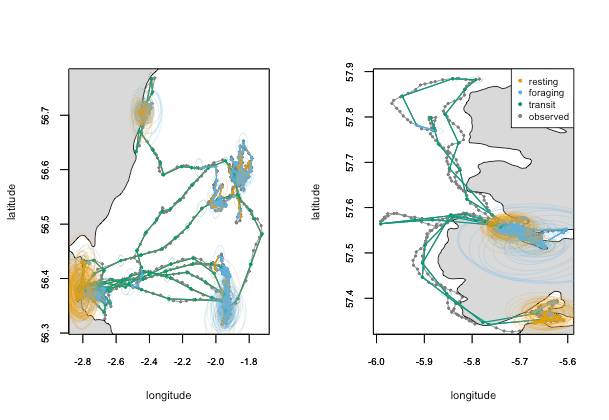
\includegraphics[width=\textwidth]{plot_harbourSeal.png}
  \caption{Two harbour seal tracks, colored by the most likely state sequence.}
  \label{fig:hsTracks}
\end{figure}
\begin{figure}[htbp]
  \centering
  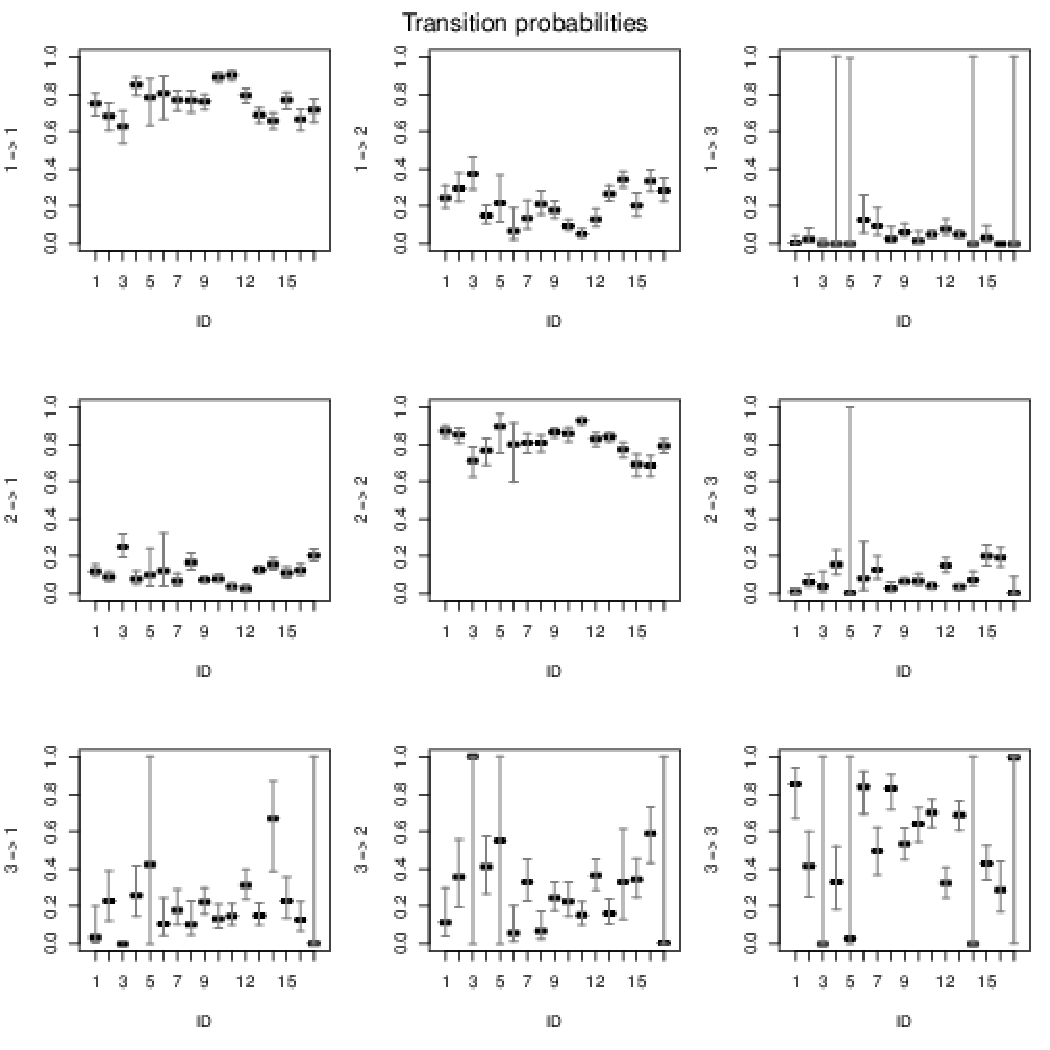
\includegraphics[width=\textwidth]{plot_harbourSealResults020}
  \caption{Estimated individual-level state transition probabilities for the harbour seal example.}
  \label{fig:hsTPM}
\end{figure}

\subsection{Northern fulmars}
\label{sec:northernFulmar}
Using Bayesian analysis methods, \cite{PirottaEtAl2018} fit a 6-state biased random walk model to northern fulmar ({\it Fulmarus glacialis}) tracks in northern Scotland, UK.  These states included biased movements relative to a colony in Eynhallow ($59.12^\circ$ N, $3.1^\circ$ W) and fishing vessels that frequently work in the area.  \cite{PirottaEtAl2018} framed their model as having two latent state process.  Under the first state process, the direction of movement could be biased away from the colony (``sea''), towards the nearest fishing vessel (``boat''), or towards the colony (``colony''). Under the second state process, the movement mode could either be fast and directionally-persistent (``transit'') or area-restricted search (``ARS'').  Thus the six states are ``sea ARS'', ``sea transit'', ``boat ARS'', ``boat transit'', ``colony ARS'' and ``colony transit''. \cite{PirottaEtAl2018} also allowed the distance to the nearest fishing vessel and time since leaving the colony to affect state transitions to the ``boat'' and ``colony'' states.  Here we demonstrate how a very similar (but not identical) model can be implemented in \verb|momentuHMM|.

The data are provided in a Dryad repository, but these will require some additional formatting and preparation.  We first load the raw data, create the required ``ID'' column based on individual trips, convert time stamps to class \verb|POSIXct|, and project the northern fulmar (``Longitude'', ``Latitude'') and nearest fishing vessel (``Boat\_Longitude'', ``Boat\_Latitude'') locations using the \verb|sp| package:
\begin{knitrout}
\definecolor{shadecolor}{rgb}{0.969, 0.969, 0.969}\color{fgcolor}\begin{kframe}
\begin{alltt}
\hlkwd{library}\hlstd{(sp)}

\hlcom{# load data provided by Pirotta et al}
\hlstd{fulmarURL} \hlkwb{<-} \hlstr{"https://datadryad.org/stash/downloads/file_stream/45899"}
\hlstd{raw_data} \hlkwb{<-} \hlkwd{read.csv}\hlstd{(}\hlkwd{url}\hlstd{(fulmarURL),}
                     \hlkwc{stringsAsFactors} \hlstd{=} \hlnum{FALSE}\hlstd{)}

\hlstd{raw_data}\hlopt{$}\hlstd{ID} \hlkwb{<-} \hlstd{raw_data}\hlopt{$}\hlstd{tripID}
\hlstd{raw_data}\hlopt{$}\hlstd{Date} \hlkwb{<-} \hlkwd{as.POSIXct}\hlstd{(raw_data}\hlopt{$}\hlstd{Date,}\hlkwc{tz}\hlstd{=}\hlstr{"UTC"}\hlstd{,}
                            \hlkwc{format}\hlstd{=}\hlstr{"%d/%m/%Y %H:%M"}\hlstd{)}

\hlcom{# project data}
\hlstd{oldProj} \hlkwb{<-} \hlkwd{CRS}\hlstd{(}\hlstr{"+proj=longlat +datum=WGS84"}\hlstd{)}
\hlstd{newProj} \hlkwb{<-} \hlkwd{CRS}\hlstd{(}\hlstr{"+init=epsg:27700"}\hlstd{)}
\hlkwd{coordinates}\hlstd{(raw_data)} \hlkwb{<-} \hlkwd{c}\hlstd{(}\hlstr{"Longitude"}\hlstd{,}\hlstr{"Latitude"}\hlstd{)}
\hlkwd{proj4string}\hlstd{(raw_data)} \hlkwb{<-} \hlstd{oldProj}
\hlstd{raw_data} \hlkwb{<-} \hlkwd{as.data.frame}\hlstd{(}\hlkwd{spTransform}\hlstd{(raw_data, newProj))}

\hlkwd{coordinates}\hlstd{(raw_data)} \hlkwb{<-} \hlkwd{c}\hlstd{(}\hlstr{"Boat_Longitude"}\hlstd{,}\hlstr{"Boat_Latitude"}\hlstd{)}
\hlkwd{proj4string}\hlstd{(raw_data)} \hlkwb{<-} \hlstd{oldProj}
\hlstd{raw_data} \hlkwb{<-} \hlkwd{as.data.frame}\hlstd{(}\hlkwd{spTransform}\hlstd{(raw_data, newProj))}
\end{alltt}
\end{kframe}
\end{knitrout}
For movements away from the colony (``sea ARS'' and ``sea transit''), \cite{PirottaEtAl2018} included bias in the direction of the farthest location from the colony for a given trip. We can use the \verb|centers| argument of \verb|prepData| to identify these locations  (``max\_dist'') and then calculate the expected angle for the ``sea'' states (``sea.angle'') using \verb|momentuHMM:::distAngle|:
\begin{knitrout}
\definecolor{shadecolor}{rgb}{0.969, 0.969, 0.969}\color{fgcolor}\begin{kframe}
\begin{alltt}
\hlcom{# use prepData to calculate colony distance covariate ('sea.angle')}
\hlstd{colony} \hlkwb{<-} \hlkwd{data.frame}\hlstd{(}\hlkwc{x} \hlstd{=} \hlopt{-}\hlnum{3.1}\hlstd{,} \hlkwc{y} \hlstd{=} \hlnum{59.12}\hlstd{)}
\hlkwd{coordinates}\hlstd{(colony)} \hlkwb{<-} \hlkwd{c}\hlstd{(}\hlstr{"x"}\hlstd{,} \hlstr{"y"}\hlstd{)}
\hlkwd{proj4string}\hlstd{(colony)} \hlkwb{<-} \hlstd{oldProj}
\hlstd{colony} \hlkwb{<-} \hlkwd{as.matrix}\hlstd{(}\hlkwd{as.data.frame}\hlstd{(}\hlkwd{spTransform}\hlstd{(colony, newProj)))}
\hlkwd{rownames}\hlstd{(colony)} \hlkwb{<-} \hlstr{"colony"}
\hlstd{colony_dist} \hlkwb{<-} \hlkwd{prepData}\hlstd{(raw_data,} \hlkwc{coordNames} \hlstd{=} \hlkwd{c}\hlstd{(}\hlstr{"Longitude"}\hlstd{,}\hlstr{"Latitude"}\hlstd{),}
                        \hlkwc{centers} \hlstd{= colony)}

\hlcom{# calculate "sea" mean angle covariate}
\hlstd{sea.angle} \hlkwb{<-} \hlkwa{NULL}
\hlkwa{for}\hlstd{(id} \hlkwa{in} \hlkwd{unique}\hlstd{(colony_dist}\hlopt{$}\hlstd{ID)) \{}
  \hlstd{idat} \hlkwb{<-} \hlkwd{subset}\hlstd{(colony_dist,ID}\hlopt{==}\hlstd{id)}
  \hlstd{nbSubObs} \hlkwb{<-} \hlkwd{length}\hlstd{(}\hlkwd{which}\hlstd{(colony_dist}\hlopt{$}\hlstd{ID}\hlopt{==}\hlstd{id))}
  \hlstd{max_dist} \hlkwb{<-} \hlkwd{as.numeric}\hlstd{(idat[}\hlkwd{which.max}\hlstd{(idat}\hlopt{$}\hlstd{colony.dist),}\hlkwd{c}\hlstd{(}\hlstr{"x"}\hlstd{,}\hlstr{"y"}\hlstd{)])}
  \hlstd{max_angle} \hlkwb{<-} \hlstd{momentuHMM}\hlopt{:::}\hlkwd{distAngle}\hlstd{(colony,colony,max_dist)[}\hlnum{2}\hlstd{]}
  \hlstd{sea.angle} \hlkwb{<-} \hlkwd{c}\hlstd{(sea.angle,} \hlkwd{rep}\hlstd{(max_angle,nbSubObs))}
\hlstd{\}}
\hlstd{raw_data}\hlopt{$}\hlstd{sea.angle} \hlkwb{<-} \hlstd{sea.angle}
\end{alltt}
\end{kframe}
\end{knitrout}

Next we calculate the time since leaving colony covariate (``time''):
\begin{knitrout}
\definecolor{shadecolor}{rgb}{0.969, 0.969, 0.969}\color{fgcolor}\begin{kframe}
\begin{alltt}
\hlcom{# calculate time since left colony covariate ('time')}
\hlstd{time} \hlkwb{<-} \hlstd{aInd} \hlkwb{<-} \hlkwa{NULL}
\hlkwa{for}\hlstd{(id} \hlkwa{in} \hlkwd{unique}\hlstd{(raw_data}\hlopt{$}\hlstd{ID)) \{}
  \hlstd{idInd} \hlkwb{<-} \hlkwd{which}\hlstd{(raw_data}\hlopt{$}\hlstd{ID}\hlopt{==}\hlstd{id)}
  \hlstd{aInd} \hlkwb{<-} \hlkwd{c}\hlstd{(aInd,idInd[}\hlnum{1}\hlstd{])}
  \hlstd{nbSubObs} \hlkwb{<-} \hlkwd{length}\hlstd{(idInd)}
  \hlstd{time} \hlkwb{<-} \hlkwd{c}\hlstd{(time, (}\hlnum{1}\hlopt{:}\hlstd{nbSubObs)}\hlopt{/}\hlstd{nbSubObs)}
\hlstd{\}}
\hlstd{raw_data}\hlopt{$}\hlstd{time} \hlkwb{<-} \hlstd{time}
\end{alltt}
\end{kframe}
\end{knitrout}

To complete our data preparation, we convert the nearest fishing vessel data to the \verb|centriods| argument format and use \verb|prepData| to calculate step lengths, turn angles, and our ``sea'', ``boat'', and ``colony'' covariates:
\begin{knitrout}
\definecolor{shadecolor}{rgb}{0.969, 0.969, 0.969}\color{fgcolor}\begin{kframe}
\begin{alltt}
\hlcom{# get boat data into centroids argument format}
\hlstd{boat_data} \hlkwb{<-} \hlkwd{list}\hlstd{(}\hlkwc{boat}\hlstd{=}\hlkwd{data.frame}\hlstd{(}\hlkwc{Date} \hlstd{= raw_data}\hlopt{$}\hlstd{Date,}
                                  \hlkwc{x} \hlstd{= raw_data}\hlopt{$}\hlstd{Boat_Longitude,}
                                  \hlkwc{y} \hlstd{= raw_data}\hlopt{$}\hlstd{Boat_Latitude))}

\hlcom{# format and merge all data and covariates for analysis}
\hlstd{fulmar_data} \hlkwb{<-} \hlkwd{prepData}\hlstd{(raw_data,} \hlkwc{coordNames} \hlstd{=} \hlkwd{c}\hlstd{(}\hlstr{"Longitude"}\hlstd{,}\hlstr{"Latitude"}\hlstd{),}
                        \hlkwc{centers} \hlstd{= colony,}
                        \hlkwc{centroids} \hlstd{= boat_data,}
                        \hlkwc{covNames} \hlstd{=} \hlstr{"time"}\hlstd{,}
                        \hlkwc{angleCovs} \hlstd{=} \hlstr{"sea.angle"}\hlstd{)}

\hlcom{# momentuHMM doesn't like data streams and covariates to have same name, }
\hlcom{# so create identical data column with different name}
\hlstd{fulmar_data}\hlopt{$}\hlstd{d} \hlkwb{<-} \hlstd{fulmar_data}\hlopt{$}\hlstd{boat.dist}

\hlcom{# standarize boat.dist covariate}
\hlstd{fulmar_data}\hlopt{$}\hlstd{boat.dist} \hlkwb{<-} \hlkwd{scale}\hlstd{(fulmar_data}\hlopt{$}\hlstd{boat.dist)}
\end{alltt}
\end{kframe}
\end{knitrout}
Note that we use the \verb|centers| argument for the colony (because its location is static) and the \verb|centroids| argument for the nearest fishing vessel (because its location is dynamic).  

Now that we've formatted the data, we're ready to specify the 6-state HMM. Using 10 min time steps, \cite{PirottaEtAl2018} included three data streams in their model: step length (``step''), turn angle (``angle''), and distance to nearest boat (``d'').  These were respectively modelled using Weibull, wrapped Cauchy, and log-normal distributions:
\begin{knitrout}
\definecolor{shadecolor}{rgb}{0.969, 0.969, 0.969}\color{fgcolor}\begin{kframe}
\begin{alltt}
\hlstd{nbStates} \hlkwb{<-} \hlnum{6}

\hlstd{stateNames} \hlkwb{<-} \hlkwd{c}\hlstd{(}\hlstr{"seaARS"}\hlstd{,} \hlstr{"seaTr"}\hlstd{,}
                \hlstr{"boatARS"}\hlstd{,} \hlstr{"boatTr"}\hlstd{,}
                \hlstr{"colonyARS"}\hlstd{,} \hlstr{"colonyTr"}\hlstd{)}

\hlstd{dist} \hlkwb{<-} \hlkwd{list}\hlstd{(}\hlkwc{step} \hlstd{=} \hlstr{"weibull"}\hlstd{,}
             \hlkwc{angle} \hlstd{=} \hlstr{"wrpcauchy"}\hlstd{,}
             \hlkwc{d} \hlstd{=} \hlstr{"lnorm"}\hlstd{)}
\end{alltt}
\end{kframe}
\end{knitrout}

Similar to the harbour seal example (section \ref{sec:harbourSeal}), \cite{PirottaEtAl2018} used relational parameter constraints that can be specified in \verb|momentuHMM| using pseudo-design matrices:
\begin{knitrout}
\definecolor{shadecolor}{rgb}{0.969, 0.969, 0.969}\color{fgcolor}\begin{kframe}
\begin{alltt}
\hlcom{# specify data stream probability distribution parameter constraints}
\hlstd{stepDM} \hlkwb{<-} \hlkwd{matrix}\hlstd{(}\hlkwd{c}\hlstd{(}\hlnum{1}\hlstd{,}\hlnum{0}\hlstd{,}\hlnum{0}\hlstd{,}\hlnum{0}\hlstd{,}
                   \hlnum{0}\hlstd{,}\hlnum{1}\hlstd{,}\hlnum{0}\hlstd{,}\hlnum{0}\hlstd{,}
                   \hlnum{1}\hlstd{,}\hlnum{0}\hlstd{,}\hlnum{0}\hlstd{,}\hlnum{0}\hlstd{,}
                   \hlnum{0}\hlstd{,}\hlnum{1}\hlstd{,}\hlnum{0}\hlstd{,}\hlnum{0}\hlstd{,}
                   \hlnum{1}\hlstd{,}\hlnum{0}\hlstd{,}\hlnum{0}\hlstd{,}\hlnum{0}\hlstd{,}
                   \hlnum{0}\hlstd{,}\hlnum{1}\hlstd{,}\hlnum{0}\hlstd{,}\hlnum{0}\hlstd{,}
                   \hlnum{0}\hlstd{,}\hlnum{0}\hlstd{,}\hlnum{1}\hlstd{,}\hlnum{0}\hlstd{,}
                   \hlnum{0}\hlstd{,}\hlnum{0}\hlstd{,}\hlnum{1}\hlstd{,}\hlnum{1}\hlstd{,}
                   \hlnum{0}\hlstd{,}\hlnum{0}\hlstd{,}\hlnum{1}\hlstd{,}\hlnum{0}\hlstd{,}
                   \hlnum{0}\hlstd{,}\hlnum{0}\hlstd{,}\hlnum{1}\hlstd{,}\hlnum{1}\hlstd{,}
                   \hlnum{0}\hlstd{,}\hlnum{0}\hlstd{,}\hlnum{1}\hlstd{,}\hlnum{0}\hlstd{,}
                   \hlnum{0}\hlstd{,}\hlnum{0}\hlstd{,}\hlnum{1}\hlstd{,}\hlnum{1}\hlstd{),}\hlnum{2}\hlopt{*}\hlstd{nbStates,}\hlnum{4}\hlstd{,}\hlkwc{byrow}\hlstd{=}\hlnum{TRUE}\hlstd{,}
                 \hlkwc{dimnames}\hlstd{=}\hlkwd{list}\hlstd{(}\hlkwd{c}\hlstd{(}\hlkwd{paste0}\hlstd{(}\hlstr{"shape_"}\hlstd{,}\hlnum{1}\hlopt{:}\hlstd{nbStates),}
                                 \hlkwd{paste0}\hlstd{(}\hlstr{"scale_"}\hlstd{,}\hlnum{1}\hlopt{:}\hlstd{nbStates)),}
                               \hlkwd{c}\hlstd{(}\hlstr{"shape:ARS"}\hlstd{,}\hlstr{"shape:Tr"}\hlstd{,}
                                 \hlstr{"scale:(Intercept)"}\hlstd{,}\hlstr{"scale:Tr"}\hlstd{)))}

\hlcom{# constrain scale parameters such that Tr > ARS }
\hlstd{stepworkBounds} \hlkwb{<-} \hlkwd{matrix}\hlstd{(}\hlkwd{c}\hlstd{(}\hlopt{-}\hlnum{Inf}\hlstd{,}\hlnum{Inf}\hlstd{,}
                           \hlopt{-}\hlnum{Inf}\hlstd{,}\hlnum{Inf}\hlstd{,}
                           \hlopt{-}\hlnum{Inf}\hlstd{,}\hlnum{Inf}\hlstd{,}
                           \hlnum{0}\hlstd{,}\hlnum{Inf}\hlstd{),}\hlkwd{ncol}\hlstd{(stepDM),}\hlnum{2}\hlstd{,}\hlkwc{byrow}\hlstd{=}\hlnum{TRUE}\hlstd{,}
                         \hlkwc{dimnames}\hlstd{=}\hlkwd{list}\hlstd{(}\hlkwd{colnames}\hlstd{(stepDM),}\hlkwd{c}\hlstd{(}\hlstr{"lower"}\hlstd{,}\hlstr{"upper"}\hlstd{)))}

\hlcom{# include trip-level effects on angle mean concentration parameter}
\hlstd{nbTrips} \hlkwb{<-} \hlkwd{length}\hlstd{(}\hlkwd{unique}\hlstd{(fulmar_data}\hlopt{$}\hlstd{ID))}
\hlstd{angleDM} \hlkwb{<-} \hlkwd{matrix}\hlstd{(}\hlkwd{c}\hlstd{(}\hlstr{"sea.angle"}\hlstd{,}\hlnum{0}\hlstd{,}\hlnum{0}\hlstd{,}\hlnum{0}\hlstd{,}\hlnum{0}\hlstd{,}\hlkwd{rep}\hlstd{(}\hlnum{0}\hlstd{,}\hlnum{2}\hlopt{*}\hlstd{nbTrips),}
                    \hlstr{"sea.angle"}\hlstd{,}\hlnum{0}\hlstd{,}\hlnum{0}\hlstd{,}\hlnum{0}\hlstd{,}\hlnum{0}\hlstd{,}\hlkwd{rep}\hlstd{(}\hlnum{0}\hlstd{,}\hlnum{2}\hlopt{*}\hlstd{nbTrips),}
                    \hlnum{0}\hlstd{,}\hlstr{"boat.angle"}\hlstd{,}\hlnum{0}\hlstd{,}\hlnum{0}\hlstd{,}\hlnum{0}\hlstd{,}\hlkwd{rep}\hlstd{(}\hlnum{0}\hlstd{,}\hlnum{2}\hlopt{*}\hlstd{nbTrips),}
                    \hlnum{0}\hlstd{,}\hlstr{"boat.angle"}\hlstd{,}\hlnum{0}\hlstd{,}\hlnum{0}\hlstd{,}\hlnum{0}\hlstd{,}\hlkwd{rep}\hlstd{(}\hlnum{0}\hlstd{,}\hlnum{2}\hlopt{*}\hlstd{nbTrips),}
                    \hlnum{0}\hlstd{,}\hlnum{0}\hlstd{,}\hlstr{"colony.angle"}\hlstd{,}\hlnum{0}\hlstd{,}\hlnum{0}\hlstd{,}\hlkwd{rep}\hlstd{(}\hlnum{0}\hlstd{,}\hlnum{2}\hlopt{*}\hlstd{nbTrips),}
                    \hlnum{0}\hlstd{,}\hlnum{0}\hlstd{,}\hlstr{"colony.angle"}\hlstd{,}\hlnum{0}\hlstd{,}\hlnum{0}\hlstd{,}\hlkwd{rep}\hlstd{(}\hlnum{0}\hlstd{,}\hlnum{2}\hlopt{*}\hlstd{nbTrips),}
                    \hlnum{0}\hlstd{,}\hlnum{0}\hlstd{,}\hlnum{0}\hlstd{,}\hlnum{1}\hlstd{,}\hlnum{0}\hlstd{,}\hlkwd{paste0}\hlstd{(}\hlstr{"ID"}\hlstd{,}\hlnum{1}\hlopt{:}\hlstd{nbTrips),}\hlkwd{rep}\hlstd{(}\hlnum{0}\hlstd{,nbTrips),}
                    \hlnum{0}\hlstd{,}\hlnum{0}\hlstd{,}\hlnum{0}\hlstd{,}\hlnum{1}\hlstd{,}\hlnum{1}\hlstd{,}\hlkwd{paste0}\hlstd{(}\hlstr{"ID"}\hlstd{,}\hlnum{1}\hlopt{:}\hlstd{nbTrips),}\hlkwd{paste0}\hlstd{(}\hlstr{"ID"}\hlstd{,}\hlnum{1}\hlopt{:}\hlstd{nbTrips),}
                    \hlnum{0}\hlstd{,}\hlnum{0}\hlstd{,}\hlnum{0}\hlstd{,}\hlnum{1}\hlstd{,}\hlnum{0}\hlstd{,}\hlkwd{rep}\hlstd{(}\hlnum{0}\hlstd{,}\hlnum{2}\hlopt{*}\hlstd{nbTrips),}
                    \hlnum{0}\hlstd{,}\hlnum{0}\hlstd{,}\hlnum{0}\hlstd{,}\hlnum{1}\hlstd{,}\hlnum{1}\hlstd{,}\hlkwd{rep}\hlstd{(}\hlnum{0}\hlstd{,}\hlnum{2}\hlopt{*}\hlstd{nbTrips),}
                    \hlnum{0}\hlstd{,}\hlnum{0}\hlstd{,}\hlnum{0}\hlstd{,}\hlnum{1}\hlstd{,}\hlnum{0}\hlstd{,}\hlkwd{rep}\hlstd{(}\hlnum{0}\hlstd{,}\hlnum{2}\hlopt{*}\hlstd{nbTrips),}
                    \hlnum{0}\hlstd{,}\hlnum{0}\hlstd{,}\hlnum{0}\hlstd{,}\hlnum{1}\hlstd{,}\hlnum{1}\hlstd{,}\hlkwd{rep}\hlstd{(}\hlnum{0}\hlstd{,}\hlnum{2}\hlopt{*}\hlstd{nbTrips)),}\hlnum{2}\hlopt{*}\hlstd{nbStates,}\hlnum{3}\hlopt{+}\hlnum{2}\hlopt{+}\hlnum{2}\hlopt{*}\hlstd{nbTrips,}\hlkwc{byrow}\hlstd{=}\hlnum{TRUE}\hlstd{,}
                  \hlkwc{dimnames}\hlstd{=}\hlkwd{list}\hlstd{(}\hlkwd{c}\hlstd{(}\hlkwd{paste0}\hlstd{(}\hlstr{"mean_"}\hlstd{,}\hlnum{1}\hlopt{:}\hlstd{nbStates),}
                                  \hlkwd{paste0}\hlstd{(}\hlstr{"concentration_"}\hlstd{,}\hlnum{1}\hlopt{:}\hlstd{nbStates)),}
                                \hlkwd{c}\hlstd{(}\hlstr{"mean:sea"}\hlstd{,}\hlstr{"mean:boat"}\hlstd{,}\hlstr{"mean:colony"}\hlstd{,}
                                  \hlstr{"concentration:(Intercept)"}\hlstd{,}\hlstr{"concentration:Tr"}\hlstd{,}
                                  \hlkwd{paste0}\hlstd{(}\hlstr{"concentration:ID"}\hlstd{,}\hlnum{1}\hlopt{:}\hlstd{nbTrips,}\hlstr{":(Intercept)"}\hlstd{),}
                                  \hlkwd{paste0}\hlstd{(}\hlstr{"concentration:ID"}\hlstd{,}\hlnum{1}\hlopt{:}\hlstd{nbTrips,}\hlstr{":Tr"}\hlstd{))))}

\hlcom{# constrain concentration parameters such that Tr > ARS }
\hlstd{angleworkBounds} \hlkwb{<-} \hlkwd{matrix}\hlstd{(}\hlkwd{c}\hlstd{(}\hlopt{-}\hlnum{Inf}\hlstd{,}\hlnum{Inf}\hlstd{,}
                            \hlopt{-}\hlnum{Inf}\hlstd{,}\hlnum{Inf}\hlstd{,}
                            \hlopt{-}\hlnum{Inf}\hlstd{,}\hlnum{Inf}\hlstd{,}
                            \hlopt{-}\hlnum{Inf}\hlstd{,}\hlnum{Inf}\hlstd{,}
                            \hlnum{0}\hlstd{,}\hlnum{Inf}\hlstd{,}
                            \hlkwd{rep}\hlstd{(}\hlkwd{c}\hlstd{(}\hlopt{-}\hlnum{Inf}\hlstd{,}\hlnum{Inf}\hlstd{),nbTrips),}
                            \hlkwd{rep}\hlstd{(}\hlkwd{c}\hlstd{(}\hlnum{0}\hlstd{,}\hlnum{Inf}\hlstd{),nbTrips)),}\hlkwd{ncol}\hlstd{(angleDM),}\hlnum{2}\hlstd{,}\hlkwc{byrow}\hlstd{=}\hlnum{TRUE}\hlstd{,}
                         \hlkwc{dimnames}\hlstd{=}\hlkwd{list}\hlstd{(}\hlkwd{colnames}\hlstd{(angleDM),}\hlkwd{c}\hlstd{(}\hlstr{"lower"}\hlstd{,}\hlstr{"upper"}\hlstd{)))}

\hlstd{dDM} \hlkwb{<-} \hlkwd{matrix}\hlstd{(}\hlkwd{c}\hlstd{(}\hlnum{1}\hlstd{,}\hlnum{1}\hlstd{,}\hlnum{0}\hlstd{,}\hlnum{0}\hlstd{,}
                \hlnum{1}\hlstd{,}\hlnum{1}\hlstd{,}\hlnum{0}\hlstd{,}\hlnum{0}\hlstd{,}
                \hlnum{1}\hlstd{,}\hlnum{0}\hlstd{,}\hlnum{0}\hlstd{,}\hlnum{0}\hlstd{,}
                \hlnum{1}\hlstd{,}\hlnum{0}\hlstd{,}\hlnum{0}\hlstd{,}\hlnum{0}\hlstd{,}
                \hlnum{1}\hlstd{,}\hlnum{1}\hlstd{,}\hlnum{0}\hlstd{,}\hlnum{0}\hlstd{,}
                \hlnum{1}\hlstd{,}\hlnum{1}\hlstd{,}\hlnum{0}\hlstd{,}\hlnum{0}\hlstd{,}
                \hlnum{0}\hlstd{,}\hlnum{0}\hlstd{,}\hlnum{1}\hlstd{,}\hlnum{1}\hlstd{,}
                \hlnum{0}\hlstd{,}\hlnum{0}\hlstd{,}\hlnum{1}\hlstd{,}\hlnum{1}\hlstd{,}
                \hlnum{0}\hlstd{,}\hlnum{0}\hlstd{,}\hlnum{1}\hlstd{,}\hlnum{0}\hlstd{,}
                \hlnum{0}\hlstd{,}\hlnum{0}\hlstd{,}\hlnum{1}\hlstd{,}\hlnum{0}\hlstd{,}
                \hlnum{0}\hlstd{,}\hlnum{0}\hlstd{,}\hlnum{1}\hlstd{,}\hlnum{1}\hlstd{,}
                \hlnum{0}\hlstd{,}\hlnum{0}\hlstd{,}\hlnum{1}\hlstd{,}\hlnum{1}\hlstd{),}\hlnum{2}\hlopt{*}\hlstd{nbStates,}\hlnum{4}\hlstd{,}\hlkwc{byrow}\hlstd{=}\hlnum{TRUE}\hlstd{,}
              \hlkwc{dimnames}\hlstd{=}\hlkwd{list}\hlstd{(}\hlkwd{c}\hlstd{(}\hlkwd{paste0}\hlstd{(}\hlstr{"location_"}\hlstd{,}\hlnum{1}\hlopt{:}\hlstd{nbStates),}
                              \hlkwd{paste0}\hlstd{(}\hlstr{"scale_"}\hlstd{,}\hlnum{1}\hlopt{:}\hlstd{nbStates)),}
                            \hlkwd{c}\hlstd{(}\hlstr{"location:(Intercept)"}\hlstd{,}\hlstr{"location:noboat"}\hlstd{,}
                              \hlstr{"scale:(Intercept)"}\hlstd{,}\hlstr{"scale:noboat"}\hlstd{)))}

\hlcom{# constrain location and scale parameters such that sea and colony > boat}
\hlstd{dworkBounds} \hlkwb{<-} \hlkwd{matrix}\hlstd{(}\hlkwd{c}\hlstd{(}\hlopt{-}\hlnum{Inf}\hlstd{,}\hlnum{Inf}\hlstd{,}
                        \hlnum{0}\hlstd{,}\hlnum{Inf}\hlstd{,}
                        \hlopt{-}\hlnum{Inf}\hlstd{,}\hlnum{Inf}\hlstd{,}
                        \hlnum{0}\hlstd{,}\hlnum{Inf}\hlstd{),}\hlkwd{ncol}\hlstd{(dDM),}\hlnum{2}\hlstd{,}\hlkwc{byrow}\hlstd{=}\hlnum{TRUE}\hlstd{,}
                      \hlkwc{dimnames}\hlstd{=}\hlkwd{list}\hlstd{(}\hlkwd{colnames}\hlstd{(dDM),}\hlkwd{c}\hlstd{(}\hlstr{"lower"}\hlstd{,}\hlstr{"upper"}\hlstd{)))}

\hlstd{DM} \hlkwb{<-} \hlkwd{list}\hlstd{(}\hlkwc{step} \hlstd{= stepDM,} \hlkwc{angle} \hlstd{= angleDM,} \hlkwc{d} \hlstd{= dDM)}

\hlstd{workBounds} \hlkwb{<-} \hlkwd{list}\hlstd{(}\hlkwc{step} \hlstd{= stepworkBounds,}
                   \hlkwc{angle} \hlstd{= angleworkBounds,}
                   \hlkwc{d} \hlstd{= dworkBounds)}
\end{alltt}
\end{kframe}
\end{knitrout}
To complete our model specification, we use the \verb|toState| special function to model transitions to the ``boat'' and ``colony'' states as a function of distance to nearest fishing vessel (``boat.dist'') and time since leaving colony (``time''), respectively.  Following \cite{PirottaEtAl2018}, we will use the \verb|knownStates| argument to fix the initial state to ``sea transit''.  We will also use the \verb|fixPar| argument to fix the initial state probabilities (because we are assuming these are known) and, as in section \ref{sec:groupModel}, constrain the model to a biased random walk by fixing the mean angle working scale parameters to a large positive value:
\begin{knitrout}
\definecolor{shadecolor}{rgb}{0.969, 0.969, 0.969}\color{fgcolor}\begin{kframe}
\begin{alltt}
\hlcom{# state transition formula similar to Pirotta et al}
\hlstd{formula} \hlkwb{<-} \hlopt{~} \hlkwd{toState3}\hlstd{(boat.dist)} \hlopt{+} \hlkwd{toState4}\hlstd{(boat.dist)} \hlopt{+}
             \hlkwd{toState5}\hlstd{(time)} \hlopt{+} \hlkwd{toState6}\hlstd{(time)}

\hlcom{# specify knownStates}
\hlcom{# Priotta et al assumed all animals start in state 2 ('seaTr')}
\hlstd{knownStates} \hlkwb{<-} \hlkwd{rep}\hlstd{(}\hlnum{NA}\hlstd{,}\hlkwd{nrow}\hlstd{(fulmar_data))}
\hlstd{knownStates[aInd]} \hlkwb{<-} \hlnum{2}

\hlcom{# fix delta_2 = 1 because assuming initial state is known for each track}
\hlstd{fixPar} \hlkwb{<-} \hlkwd{list}\hlstd{(}\hlkwc{delta}\hlstd{=}\hlkwd{c}\hlstd{(}\hlnum{100}\hlstd{,}\hlkwd{rep}\hlstd{(}\hlnum{0}\hlstd{,nbStates}\hlopt{-}\hlnum{2}\hlstd{)))}
\hlstd{fixPar}\hlopt{$}\hlstd{delta} \hlkwb{<-} \hlkwd{exp}\hlstd{(}\hlkwd{c}\hlstd{(}\hlnum{0}\hlstd{,fixPar}\hlopt{$}\hlstd{delta))}\hlopt{/}\hlkwd{sum}\hlstd{(}\hlkwd{exp}\hlstd{(}\hlkwd{c}\hlstd{(}\hlnum{0}\hlstd{,fixPar}\hlopt{$}\hlstd{delta)))}
\hlcom{# Constrain model to BRW (instead of BCRW)}
\hlstd{fixPar}\hlopt{$}\hlstd{angle} \hlkwb{<-} \hlkwd{c}\hlstd{(}\hlkwd{rep}\hlstd{(}\hlnum{1.e+7}\hlstd{,} \hlnum{3}\hlstd{),} \hlkwd{rep}\hlstd{(}\hlnum{NA}\hlstd{,} \hlnum{2}\hlopt{+}\hlnum{2}\hlopt{*}\hlstd{nbTrips))}
\end{alltt}
\end{kframe}
\end{knitrout}
\noindent Lastly, we used the \verb|betaCons| argument to impose similar constraints as \cite{PirottaEtAl2018} for the transition probability parameters. We accomplish this by using \verb|betaCons| to set the transition probability working parameter intercept terms equal among the three ``ARS'' states and the three ``transit'' states. We also use \verb|betaCons| to constrain the effects of `boat.dist' and `time' to be identical for each of the two movement modes (``ARS'' and ``transit'') within each of the three biased movement states (``sea'', ``boat'', and ``colony''). \verb|betaCons| must be a matrix of the same dimension as \verb|beta0| and be composed of integers, where each beta working parameter is sequentially indexed in a column-wise fashion. Equality constraints can then be incorporated by having parameters share the same index. In this example we have:

\begin{knitrout}\small
\definecolor{shadecolor}{rgb}{0.969, 0.969, 0.969}\color{fgcolor}\begin{kframe}
\begin{alltt}
\hlstd{betaCons}
\end{alltt}
\begin{verbatim}
##             1 -> 2 1 -> 3 1 -> 4 1 -> 5 1 -> 6 2 -> 1 2 -> 3 2 -> 4 2 -> 5
## (Intercept)      1      4      1      4      1     16     16     22     16
## boat.dist        2      5      5     11     14     17      5      5     26
## time             3      6      9     12     12     18     21     24     12
##             2 -> 6 3 -> 1 3 -> 2 3 -> 4 3 -> 5 3 -> 6 4 -> 1 4 -> 2 4 -> 3
## (Intercept)     22      4      1      1      4      1     16     22     16
## boat.dist       29     32     35     38     41     44     47     50     38
## time            12     33     36     39     42     42     48     51     54
##             4 -> 5 4 -> 6 5 -> 1 5 -> 2 5 -> 3 5 -> 4 5 -> 6 6 -> 1 6 -> 2
## (Intercept)     16     22      4      1      4      1      1     16     22
## boat.dist       56     59     62     65     68     68     74     77     80
## time            42     42     63     66     69     72     75     78     81
##             6 -> 3 6 -> 4 6 -> 5
## (Intercept)     16     22     16
## boat.dist       68     68     89
## time            84     87     75
\end{verbatim}
\end{kframe}
\end{knitrout}
\noindent Again, \verb|betaCons| constrains any of the transition probability matrix working parameters with the same index to be equal to one another. For example, all of the intercept terms indexed by a `1' ($1 \rightarrow 2$, $1 \rightarrow 4$, $1 \rightarrow 6$, $3 \rightarrow 2$, $3 \rightarrow 4$, $3 \rightarrow 6$, $5 \rightarrow 2$, $5 \rightarrow 4$, and $5 \rightarrow 6$) are equal, and these terms correspond to the transitions from the ``ARS'' movement mode (states 1, 3, and 5) to the ``transit'' movement mode (states 2, 4, and 6). Similarly, all of the intercept terms indexed by a `16' are equal and correspond to the transitions from the ``transit'' movement mode to the ``ARS'' movement mode. For further details on the \verb|betaCons| argument, see the \verb|fitHMM| help file and the northern fulmar example code in the ``vignettes'' source directory.

Now we are ready to fit our 6-state HMM:
\begin{knitrout}
\definecolor{shadecolor}{rgb}{0.969, 0.969, 0.969}\color{fgcolor}\begin{kframe}
\begin{alltt}
\hlstd{m2} \hlkwb{<-} \hlkwd{fitHMM}\hlstd{(fulmar_data, nbStates, dist,}
             \hlkwc{Par0} \hlstd{= Par0}\hlopt{$}\hlstd{Par,} \hlkwc{beta0} \hlstd{= Par0}\hlopt{$}\hlstd{beta0,}
             \hlkwc{formula} \hlstd{= formula,}
             \hlkwc{estAngleMean} \hlstd{=} \hlkwd{list}\hlstd{(}\hlkwc{angle} \hlstd{=} \hlnum{TRUE}\hlstd{),}
             \hlkwc{circularAngleMean} \hlstd{=} \hlkwd{list}\hlstd{(}\hlkwc{angle} \hlstd{=} \hlnum{TRUE}\hlstd{),}
             \hlkwc{DM} \hlstd{= DM,} \hlkwc{workBounds} \hlstd{= workBounds,} \hlkwc{betaCons} \hlstd{= betaCons,}
             \hlkwc{fixPar} \hlstd{= fixPar,} \hlkwc{knownStates} \hlstd{= knownStates,}
             \hlkwc{stateNames} \hlstd{= stateNames)}
\end{alltt}
\end{kframe}
\end{knitrout}
\noindent With decent starting values, this model required about 2 min to fit on a standard desktop computer (macOS El Capitan, 2.8 GHz Intel Core i7, 16 GB RAM). For comparison, \cite{PirottaEtAl2018} required about 18 hr to fit their Bayesian model using MCMC (2.9 GHz Intel Core i7, 16 GB RAM). 

We can compare the estimated activity budgets with those of \cite{PirottaEtAl2018} using the \verb|timeInStates| function:
\begin{knitrout}
\definecolor{shadecolor}{rgb}{0.969, 0.969, 0.969}\color{fgcolor}\begin{kframe}
\begin{alltt}
\hlkwd{timeInStates}\hlstd{(m2)}
\end{alltt}
\end{kframe}
\end{knitrout}
\begin{knitrout}
\definecolor{shadecolor}{rgb}{0.969, 0.969, 0.969}\color{fgcolor}\begin{kframe}
\begin{verbatim}
##      seaARS     seaTr   boatARS     boatTr colonyARS  colonyTr
## 1 0.2582469 0.1687088 0.1705938 0.06503299 0.1677663 0.1696513
\end{verbatim}
\end{kframe}
\end{knitrout}
\noindent \cite{PirottaEtAl2018} estimated 0.28 (``seaARS''), 0.20 (``seaTr''), 0.18 (``boatARS''), 0.06 (``boatTr''), 0.12 (``colonyARS''), and 0.16 (``colonyTr''). While these are very similar, there a handful of state assignments that differ between the analyses. These differences could be attributable to several factors, including: 1) the use of informative priors in the Bayesian analysis of \cite{PirottaEtAl2018}; 2) our use of fixed trip-level effects on the ``sea'' state turn angle concentration parameters; and 3) \cite{PirottaEtAl2018} assumed the state transition probability covariates (``boat.dist'' and ``time'') only affected the movement direction states (``sea'', ``boat'', ``colony''), but in our \verb|momentuHMM| implementation the covariates can affect state transitions for both the movement direction (``sea'', ``boat'', ``colony'') and the movement mode (``ARS'', ``transit'').

We can also examine activity budgets by individual bird (which are indexed in the raw data ``birdID'' column), where it is clear that the first 3 individuals tended to spend a larger proportion of their foraging trips in the ``boat'' states:
\begin{knitrout}
\definecolor{shadecolor}{rgb}{0.969, 0.969, 0.969}\color{fgcolor}\begin{kframe}
\begin{alltt}
\hlkwd{timeInStates}\hlstd{(m2,} \hlkwc{by} \hlstd{=} \hlstr{"birdID"}\hlstd{)}
\end{alltt}
\end{kframe}
\end{knitrout}
\begin{knitrout}
\definecolor{shadecolor}{rgb}{0.969, 0.969, 0.969}\color{fgcolor}\begin{kframe}
\begin{verbatim}
##   birdID     seaARS       seaTr    boatARS     boatTr  colonyARS
## 1      1 0.35564854 0.117154812 0.22594142 0.11297071 0.09623431
## 2      2 0.14102564 0.134615385 0.28205128 0.10256410 0.25641026
## 3      3 0.08333333 0.269607843 0.35294118 0.06862745 0.04411765
## 4      4 0.49019608 0.196078431 0.00000000 0.04575163 0.05882353
## 5      5 0.61475410 0.008196721 0.00000000 0.00000000 0.30327869
## 6      6 0.00000000 0.235294118 0.05882353 0.02673797 0.32085561
##     colonyTr
## 1 0.09205021
## 2 0.08333333
## 3 0.18137255
## 4 0.20915033
## 5 0.07377049
## 6 0.35828877
\end{verbatim}
\end{kframe}
\end{knitrout}

Finally, we can create a plot similar to \cite{PirottaEtAl2018} using the \verb|plotSat| function (Figure \ref{fig:northernFulmar}):
\begin{knitrout}
\definecolor{shadecolor}{rgb}{0.969, 0.969, 0.969}\color{fgcolor}\begin{kframe}
\begin{alltt}
\hlkwd{plotSat}\hlstd{(m2,} \hlkwc{zoom} \hlstd{=} \hlnum{7}\hlstd{,} \hlkwc{shape} \hlstd{=} \hlkwd{c}\hlstd{(}\hlnum{17}\hlstd{,}\hlnum{1}\hlstd{,}\hlnum{17}\hlstd{,}\hlnum{1}\hlstd{,}\hlnum{17}\hlstd{,}\hlnum{1}\hlstd{),} \hlkwc{size} \hlstd{=} \hlnum{2}\hlstd{,}
        \hlkwc{col} \hlstd{=} \hlkwd{rep}\hlstd{(}\hlkwd{c}\hlstd{(}\hlstr{"#E69F00"}\hlstd{,} \hlstr{"#56B4E9"}\hlstd{,} \hlstr{"#009E73"}\hlstd{),} \hlkwc{each} \hlstd{=} \hlnum{2}\hlstd{),}
        \hlkwc{stateNames} \hlstd{=} \hlkwd{c}\hlstd{(}\hlstr{"sea ARS"}\hlstd{,} \hlstr{"sea Transit"}\hlstd{,}
                       \hlstr{"boat ARS"}\hlstd{,} \hlstr{"boat Transit"}\hlstd{,}
                       \hlstr{"colony ARS"}\hlstd{,} \hlstr{"colony Transit"}\hlstd{),}
        \hlkwc{projargs} \hlstd{= newProj,} \hlkwc{ask} \hlstd{=} \hlnum{FALSE}\hlstd{)}
\end{alltt}
\end{kframe}
\end{knitrout}
\begin{figure}[htbp]
  \centering
  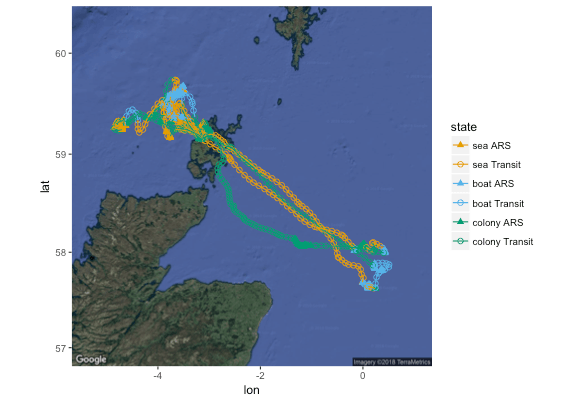
\includegraphics[width=\textwidth]{plot_northernFulmarExample.png}
  \caption{Seven northern fulmar tracks, colored by the most likely state sequence.}
  \label{fig:northernFulmar}
\end{figure}

\subsection{Pilot whales}
\label{sec:pilotWhale}

Here we demonstrate how to include individual heterogeneity in state-switching dynamics via discrete-valued random effects by fitting the 4-state (``exploratory'', ``foraging'', ``crowded'', ``directed'') mixed HHM for long-finned pilot whales described in \cite{IsojunnoEtAl2017}.  The pilot whale data consist of 11 data streams collected from 15 individuals, and, as usual, we must first prepare the data for \verb|fitHMM| using \verb|prepData|. Let's summarize our prepared data using the \verb|summary| function:
\begin{knitrout}
\definecolor{shadecolor}{rgb}{0.969, 0.969, 0.969}\color{fgcolor}\begin{kframe}
\begin{alltt}
\hlkwd{summary}\hlstd{(pilotData,} \hlkwc{dataNames}\hlstd{=}\hlkwd{names}\hlstd{(pilotData)[}\hlopt{-}\hlnum{1}\hlstd{])}
\end{alltt}
\begin{verbatim}
## HMM data for 15 individuals:
## 
## gm08_150c -- 156 observations
## gm08_154d -- 142 observations
## gm08_159a -- 192 observations
## gm09_137b -- 152 observations
## gm09_138a -- 223 observations
## gm09_156b -- 254 observations
## gm10_000a -- 119 observations
## gm10_143a -- 146 observations
## gm10_152b -- 50 observations
## gm10_157b -- 130 observations
## gm10_158d -- 148 observations
## gm13_137a -- 144 observations
## gm13_149a -- 88 observations
## gm13_169a -- 190 observations
## gm14_180a -- 180 observations
## 
## 
## Data summaries:
## 
##     dive.dur       dive.depth       GR.speed2     dive.pitchvar2 
##  Min.   : 0.14   Min.   :  0.86   Min.   :0.025   Min.   :0.010  
##  1st Qu.: 0.64   1st Qu.:  5.36   1st Qu.:0.838   1st Qu.:0.042  
##  Median : 0.81   Median :  7.08   Median :1.272   Median :0.070  
##  Mean   : 1.40   Mean   : 26.36   Mean   :1.367   Mean   :0.100  
##  3rd Qu.: 1.41   3rd Qu.: 11.73   3rd Qu.:1.732   3rd Qu.:0.121  
##  Max.   :13.75   Max.   :617.37   Max.   :8.824   Max.   :0.673  
##                                   NA's   :892     NA's   :142    
##  breath.headchange     GR.size       GR.tight     dive.CS.pres
##  Min.   :-3.12587   Min.   : 0    Min.   :0.00   Min.   :0.0  
##  1st Qu.:-0.19089   1st Qu.: 6    1st Qu.:1.00   1st Qu.:0.0  
##  Median : 0.00066   Median : 9    Median :1.00   Median :1.0  
##  Mean   :-0.00407   Mean   :11    Mean   :0.82   Mean   :0.6  
##  3rd Qu.: 0.18903   3rd Qu.:13    3rd Qu.:1.00   3rd Qu.:1.0  
##  Max.   : 3.05424   Max.   :79    Max.   :1.00   Max.   :1.0  
##  NA's   :261        NA's   :665   NA's   :1128   NA's   :905  
##   dive.SS.pres     presurf        postsurf   
##  Min.   :0.00   Min.   :0.00   Min.   :0.00  
##  1st Qu.:0.00   1st Qu.:0.00   1st Qu.:0.00  
##  Median :1.00   Median :1.00   Median :1.00  
##  Mean   :0.56   Mean   :0.74   Mean   :0.74  
##  3rd Qu.:1.00   3rd Qu.:1.00   3rd Qu.:1.00  
##  Max.   :1.00   Max.   :1.00   Max.   :1.00  
##  NA's   :905    NA's   :15     NA's   :15
\end{verbatim}
\end{kframe}
\end{knitrout}

After specifying the data stream probability distributions and starting values for the parameters \citep[based on those reported by ][]{IsojunnoEtAl2017}, let's first fit the null model with no discrete-valued individual-level random effects on the state-switching dynamics:
\begin{knitrout}
\definecolor{shadecolor}{rgb}{0.969, 0.969, 0.969}\color{fgcolor}\begin{kframe}
\begin{alltt}
\hlcom{## 11 data streams}
\hlstd{dist} \hlkwb{<-} \hlkwd{list}\hlstd{(}\hlkwc{dive.dur} \hlstd{=} \hlstr{"weibull"}\hlstd{,}
             \hlkwc{dive.depth} \hlstd{=} \hlstr{"gamma"}\hlstd{,}
             \hlkwc{GR.speed2} \hlstd{=} \hlstr{"gamma"}\hlstd{,}
             \hlkwc{dive.pitchvar2} \hlstd{=} \hlstr{"beta"}\hlstd{,}
             \hlkwc{breath.headchange} \hlstd{=} \hlstr{"vm"}\hlstd{,}
             \hlkwc{GR.size} \hlstd{=} \hlstr{"pois"}\hlstd{,}
             \hlkwc{GR.tight} \hlstd{=} \hlstr{"bern"}\hlstd{,}
             \hlkwc{dive.CS.pres} \hlstd{=} \hlstr{"bern"}\hlstd{,}
             \hlkwc{dive.SS.pres} \hlstd{=} \hlstr{"bern"}\hlstd{,}
             \hlkwc{presurf} \hlstd{=} \hlstr{"bern"}\hlstd{,}
             \hlkwc{postsurf} \hlstd{=} \hlstr{"bern"}\hlstd{)}

\hlcom{## initial values}
\hlstd{Par0} \hlkwb{<-} \hlkwd{list}\hlstd{(}\hlkwc{dive.dur} \hlstd{=} \hlkwd{c}\hlstd{(}\hlnum{1.9}\hlstd{,} \hlnum{2.72}\hlstd{,} \hlnum{1.64}\hlstd{,} \hlnum{4.21}\hlstd{,}
                          \hlnum{1.3}\hlstd{,} \hlnum{8.14}\hlstd{,} \hlnum{1.53}\hlstd{,} \hlnum{0.79}\hlstd{),}
             \hlkwc{dive.depth} \hlstd{=} \hlkwd{c}\hlstd{(}\hlnum{10.23}\hlstd{,} \hlnum{315.91}\hlstd{,} \hlnum{10.74}\hlstd{,} \hlnum{5.51}\hlstd{,}
                             \hlnum{4.93}\hlstd{,} \hlnum{233.12}\hlstd{,}  \hlnum{6.32}\hlstd{,} \hlnum{1.91}\hlstd{),}
             \hlkwc{GR.speed2} \hlstd{=} \hlkwd{c}\hlstd{(}\hlnum{1.15}\hlstd{,} \hlnum{1.32}\hlstd{,} \hlnum{1.36}\hlstd{,} \hlnum{1.57}\hlstd{,}
                           \hlnum{0.66}\hlstd{,} \hlnum{0.51}\hlstd{,} \hlnum{0.77}\hlstd{,} \hlnum{0.76}\hlstd{),}
             \hlkwc{dive.pitchvar2} \hlstd{=} \hlkwd{c}\hlstd{(} \hlnum{2.21}\hlstd{,} \hlnum{2.88}\hlstd{,}  \hlnum{1.82}\hlstd{,}  \hlnum{3.18}\hlstd{,}
                                \hlnum{17.94}\hlstd{,} \hlnum{6.04}\hlstd{,} \hlnum{16.06}\hlstd{,} \hlnum{55.36}\hlstd{),}
             \hlkwc{breath.headchange} \hlstd{=} \hlkwd{c}\hlstd{(}\hlnum{3.07}\hlstd{,} \hlnum{5.65}\hlstd{,} \hlnum{2.64}\hlstd{,} \hlnum{18.02}\hlstd{),}
             \hlkwc{GR.size} \hlstd{=} \hlkwd{c}\hlstd{(}\hlnum{6}\hlstd{,} \hlnum{7.39}\hlstd{,} \hlnum{20.39}\hlstd{,} \hlnum{9.52}\hlstd{),}
             \hlkwc{GR.tight} \hlstd{=} \hlkwd{c}\hlstd{(}\hlnum{0.89}\hlstd{,} \hlnum{0.66}\hlstd{,} \hlnum{0.76}\hlstd{,} \hlnum{0.81}\hlstd{),}
             \hlkwc{dive.CS.pres} \hlstd{=} \hlkwd{c}\hlstd{(}\hlnum{0.76}\hlstd{,} \hlnum{0.99}\hlstd{,} \hlnum{0.41}\hlstd{,} \hlnum{0.47}\hlstd{),}
             \hlkwc{dive.SS.pres} \hlstd{=} \hlkwd{c}\hlstd{(}\hlnum{0.72}\hlstd{,} \hlnum{0.98}\hlstd{,} \hlnum{0.39}\hlstd{,} \hlnum{0.41}\hlstd{),}
             \hlkwc{presurf} \hlstd{=} \hlkwd{c}\hlstd{(}\hlnum{0.76}\hlstd{,} \hlnum{0.99}\hlstd{,} \hlnum{0.71}\hlstd{,} \hlnum{0.71}\hlstd{),}
             \hlkwc{postsurf} \hlstd{=} \hlkwd{c}\hlstd{(}\hlnum{0.81}\hlstd{,} \hlnum{0.96}\hlstd{,} \hlnum{0.72}\hlstd{,} \hlnum{0.66}\hlstd{))}

\hlstd{beta0} \hlkwb{<-} \hlkwd{matrix}\hlstd{(}\hlkwd{c}\hlstd{(}\hlopt{-}\hlnum{2.38}\hlstd{,} \hlopt{-}\hlnum{3.86}\hlstd{,} \hlopt{-}\hlnum{1.22}\hlstd{,}
                   \hlnum{0.21}\hlstd{,}  \hlopt{-}\hlnum{1.6}\hlstd{,} \hlopt{-}\hlnum{0.47}\hlstd{,}
                  \hlopt{-}\hlnum{3.56}\hlstd{,} \hlopt{-}\hlnum{4.15}\hlstd{,} \hlopt{-}\hlnum{2.29}\hlstd{,}
                  \hlopt{-}\hlnum{1.17}\hlstd{,} \hlopt{-}\hlnum{3.05}\hlstd{,} \hlopt{-}\hlnum{2.54}\hlstd{),}\hlkwc{nrow}\hlstd{=}\hlnum{1}\hlstd{)}

\hlstd{stateNames} \hlkwb{<-} \hlkwd{c}\hlstd{(}\hlstr{"exploratory"}\hlstd{,}\hlstr{"foraging"}\hlstd{,}\hlstr{"crowded"}\hlstd{,}\hlstr{"directed"}\hlstd{)}
\end{alltt}
\end{kframe}
\end{knitrout}
\noindent \cite{IsojunnoEtAl2017} found that model selection criteria favored models that assume the initial distribution is the stationary distribution, so we'll set \verb|stationary=TRUE|:
\begin{knitrout}
\definecolor{shadecolor}{rgb}{0.969, 0.969, 0.969}\color{fgcolor}\begin{kframe}
\begin{alltt}
\hlcom{## fit model with single mixture on TPM}
\hlstd{fitmix1} \hlkwb{<-} \hlkwd{fitHMM}\hlstd{(pilotData,} \hlkwc{nbStates}\hlstd{=}\hlnum{4}\hlstd{,} \hlkwc{dist}\hlstd{=dist,}
                  \hlkwc{Par0}\hlstd{=Par0,} \hlkwc{beta0}\hlstd{=beta0,}
                  \hlkwc{stationary}\hlstd{=}\hlnum{TRUE}\hlstd{,}
                  \hlkwc{stateNames}\hlstd{=stateNames,}
                  \hlkwc{nlmPar}\hlstd{=}\hlkwd{list}\hlstd{(}\hlkwc{hessian}\hlstd{=}\hlnum{FALSE}\hlstd{))}
\hlstd{fitmix1}
\end{alltt}
\begin{verbatim}
## Value of the maximum log-likelihood: -18510.4 
## 
## 
## dive.dur parameters:
## --------------------
##       exploratory foraging  crowded  directed
## shape    1.895587 2.719570 1.640040 4.2099390
## scale    1.301088 8.142114 1.529318 0.7911992
## 
## dive.depth parameters:
## ----------------------
##      exploratory foraging   crowded directed
## mean   10.221159 315.7408 10.752753 5.507151
## sd      4.920867 233.2394  6.325075 1.908221
## 
## GR.speed2 parameters:
## ---------------------
##      exploratory  foraging crowded  directed
## mean   1.1469499 1.3170625 1.36225 1.5706933
## sd     0.6602282 0.5121064 0.77157 0.7628831
## 
## dive.pitchvar2 parameters:
## --------------------------
##        exploratory foraging   crowded  directed
## shape1    2.205733 2.876755  1.823291  3.186465
## shape2   17.948930 6.036487 16.067474 55.491769
## 
## breath.headchange parameters:
## -----------------------------
##               exploratory foraging  crowded directed
## mean             0.000000 0.000000 0.000000  0.00000
## concentration    3.068759 5.653926 2.644184 18.04806
## 
## GR.size parameters:
## -------------------
##        exploratory foraging  crowded directed
## lambda    5.996763 7.392536 20.38838 9.522725
## 
## GR.tight parameters:
## --------------------
##      exploratory  foraging   crowded  directed
## prob   0.8885557 0.6629627 0.7609689 0.8072405
## 
## dive.CS.pres parameters:
## ------------------------
##      exploratory  foraging   crowded  directed
## prob   0.7630851 0.9892991 0.4077435 0.4703789
## 
## dive.SS.pres parameters:
## ------------------------
##      exploratory  foraging   crowded  directed
## prob   0.7167555 0.9789121 0.3955766 0.4115657
## 
## presurf parameters:
## -------------------
##      exploratory  foraging crowded  directed
## prob     0.76011 0.9924097 0.70787 0.7068425
## 
## postsurf parameters:
## --------------------
##      exploratory  foraging   crowded  directed
## prob   0.8081057 0.9619604 0.7164094 0.6568226
## 
## Regression coeffs for the transition probabilities:
## ---------------------------------------------------
##              1 -> 2    1 -> 3    1 -> 4    2 -> 1    2 -> 3     2 -> 4
## (Intercept) -2.3725 -3.871793 -1.230078 0.2005482 -1.623498 -0.4895434
##                3 -> 1    3 -> 2    3 -> 4    4 -> 1    4 -> 2    4 -> 3
## (Intercept) -3.543939 -4.120499 -2.272679 -1.163733 -3.035013 -2.539986
## 
## Transition probability matrix:
## ------------------------------
##             exploratory   foraging    crowded   directed
## exploratory  0.71106663 0.06630503 0.01480512 0.20782321
## foraging     0.40303342 0.32979502 0.06503813 0.20213342
## crowded      0.02516983 0.01414110 0.87095004 0.08973904
## directed     0.21699916 0.03340193 0.05479726 0.69480165
## 
## Initial distribution:
## ---------------------
## exploratory    foraging     crowded    directed 
##  0.36640726  0.05854032  0.22161529  0.35343713
\end{verbatim}
\end{kframe}
\end{knitrout}
\noindent (note that we've set the \verb|nlmPar| option \verb|hessian=FALSE| simply to speed up the compile time for this vignette). 

Now we'll fit a model with $K=2$ mixtures of discrete-valued individual-level random effects by setting \verb|mixtures=2|, but first we'll set some starting values based on the null model (using \verb|getPar0|) and check our model specification (using \verb|checkPar0|):
\begin{knitrout}
\definecolor{shadecolor}{rgb}{0.969, 0.969, 0.969}\color{fgcolor}\begin{kframe}
\begin{alltt}
\hlstd{Par0_mix2} \hlkwb{<-} \hlkwd{getPar0}\hlstd{(fitmix1,} \hlkwc{mixtures}\hlstd{=}\hlnum{2}\hlstd{)}
\hlstd{Par0_mix2}\hlopt{$}\hlstd{beta}\hlopt{$}\hlstd{beta[}\hlnum{1}\hlstd{,]} \hlkwb{<-} \hlkwd{c}\hlstd{(}\hlopt{-}\hlnum{2.26}\hlstd{,} \hlopt{-}\hlnum{3.93}\hlstd{,} \hlopt{-}\hlnum{0.58}\hlstd{,}
                              \hlnum{0.03}\hlstd{,} \hlopt{-}\hlnum{2.25}\hlstd{,} \hlopt{-}\hlnum{0.26}\hlstd{,}
                             \hlopt{-}\hlnum{3.38}\hlstd{,} \hlopt{-}\hlnum{4.79}\hlstd{,} \hlopt{-}\hlnum{2.82}\hlstd{,}
                             \hlopt{-}\hlnum{1.06}\hlstd{,}  \hlopt{-}\hlnum{3.3}\hlstd{,} \hlopt{-}\hlnum{3.43}\hlstd{)}
\hlstd{Par0_mix2}\hlopt{$}\hlstd{beta}\hlopt{$}\hlstd{beta[}\hlnum{2}\hlstd{,]} \hlkwb{<-} \hlkwd{c}\hlstd{(}\hlopt{-}\hlnum{2.51}\hlstd{,} \hlopt{-}\hlnum{3.32}\hlstd{,} \hlopt{-}\hlnum{2.63}\hlstd{,}
                              \hlnum{0.03}\hlstd{,} \hlopt{-}\hlnum{1.26}\hlstd{,} \hlopt{-}\hlnum{0.12}\hlstd{,}
                             \hlopt{-}\hlnum{96.8}\hlstd{,} \hlopt{-}\hlnum{3.62}\hlstd{,} \hlopt{-}\hlnum{1.75}\hlstd{,}
                             \hlopt{-}\hlnum{1.76}\hlstd{,} \hlopt{-}\hlnum{2.14}\hlstd{,} \hlopt{-}\hlnum{1.38}\hlstd{)}
\hlstd{Par0_mix2}\hlopt{$}\hlstd{beta}\hlopt{$}\hlstd{pi} \hlkwb{<-} \hlkwd{c}\hlstd{(}\hlnum{0.73}\hlstd{,} \hlnum{0.27}\hlstd{)}
\end{alltt}
\end{kframe}
\end{knitrout}
\noindent Note that because \verb|mixtures| is $>1$, the starting values for \verb|beta0| must now be specified as a list with elements named \verb|beta| (containing the starting values for the t.p.m. parameters) and/or \verb|pi| (containing the starting values for the mixture probability parameters).
\begin{knitrout}
\definecolor{shadecolor}{rgb}{0.969, 0.969, 0.969}\color{fgcolor}\begin{kframe}
\begin{alltt}
\hlcom{# check model specification}
\hlkwd{checkPar0}\hlstd{(pilotData,} \hlkwc{nbStates}\hlstd{=}\hlnum{4}\hlstd{,} \hlkwc{dist}\hlstd{=dist,}
          \hlkwc{Par0}\hlstd{=Par0_mix2}\hlopt{$}\hlstd{Par,} \hlkwc{beta0}\hlstd{=Par0_mix2}\hlopt{$}\hlstd{beta,}
          \hlkwc{stationary}\hlstd{=}\hlnum{TRUE}\hlstd{,}
          \hlkwc{mixtures}\hlstd{=}\hlnum{2}\hlstd{,}
          \hlkwc{stateNames}\hlstd{=stateNames)}
\end{alltt}
\begin{verbatim}
## 
## dive.dur parameters:
## --------------------
##       exploratory foraging  crowded  directed
## shape    1.895587 2.719570 1.640040 4.2099390
## scale    1.301088 8.142114 1.529318 0.7911992
## 
## dive.depth parameters:
## ----------------------
##      exploratory foraging   crowded directed
## mean   10.221159 315.7408 10.752753 5.507151
## sd      4.920867 233.2394  6.325075 1.908221
## 
## GR.speed2 parameters:
## ---------------------
##      exploratory  foraging crowded  directed
## mean   1.1469499 1.3170625 1.36225 1.5706933
## sd     0.6602282 0.5121064 0.77157 0.7628831
## 
## dive.pitchvar2 parameters:
## --------------------------
##        exploratory foraging   crowded  directed
## shape1    2.205733 2.876755  1.823291  3.186465
## shape2   17.948930 6.036487 16.067474 55.491769
## 
## breath.headchange parameters:
## -----------------------------
##               exploratory foraging  crowded directed
## concentration    3.068759 5.653926 2.644184 18.04806
## 
## GR.size parameters:
## -------------------
##        exploratory foraging  crowded directed
## lambda    5.996763 7.392536 20.38838 9.522725
## 
## GR.tight parameters:
## --------------------
##      exploratory  foraging   crowded  directed
## prob   0.8885557 0.6629627 0.7609689 0.8072405
## 
## dive.CS.pres parameters:
## ------------------------
##      exploratory  foraging   crowded  directed
## prob   0.7630851 0.9892991 0.4077435 0.4703789
## 
## dive.SS.pres parameters:
## ------------------------
##      exploratory  foraging   crowded  directed
## prob   0.7167555 0.9789121 0.3955766 0.4115657
## 
## presurf parameters:
## -------------------
##      exploratory  foraging crowded  directed
## prob     0.76011 0.9924097 0.70787 0.7068425
## 
## postsurf parameters:
## --------------------
##      exploratory  foraging   crowded  directed
## prob   0.8081057 0.9619604 0.7164094 0.6568226
## 
## Mixture probabilities (pi):
## ---------------------------
## mix1 mix2 
## 0.73 0.27 
## 
## Regression coeffs for the transition probabilities (beta):
## ----------------------------------------------------------
##                  1 -> 2 1 -> 3 1 -> 4 2 -> 1 2 -> 3 2 -> 4 3 -> 1 3 -> 2
## (Intercept)_mix1  -2.26  -3.93  -0.58   0.03  -2.25  -0.26  -3.38  -4.79
## (Intercept)_mix2  -2.51  -3.32  -2.63   0.03  -1.26  -0.12 -96.80  -3.62
##                  3 -> 4 4 -> 1 4 -> 2 4 -> 3
## (Intercept)_mix1  -2.82  -1.06  -3.30  -3.43
## (Intercept)_mix2  -1.75  -1.76  -2.14  -1.38
\end{verbatim}
\end{kframe}
\end{knitrout}
We can see above that by setting \verb|mixtures=2| we now have $K=2$ sets of state transition probability matrix parameters, each suffixed by a mixture label (\verb|_mix1| or \verb|_mix2|). We also now have $K=2$ mixture probability parameters $({\boldsymbol \pi})$, where the first $(\pi_1)$ corresponds to parameters suffixed with \verb|_mix1| and the second $(\pi_2)$ corresponds to parameters suffixed with \verb|_mix2|. Now let's fit the $K=2$ mixture model from \cite{IsojunnoEtAl2017}:
\begin{knitrout}
\definecolor{shadecolor}{rgb}{0.969, 0.969, 0.969}\color{fgcolor}\begin{kframe}
\begin{alltt}
\hlstd{fitmix2} \hlkwb{<-} \hlkwd{fitHMM}\hlstd{(pilotData,} \hlkwc{nbStates}\hlstd{=}\hlnum{4}\hlstd{,} \hlkwc{dist}\hlstd{=dist,}
                  \hlkwc{Par0}\hlstd{=Par0_mix2}\hlopt{$}\hlstd{Par,} \hlkwc{beta0}\hlstd{=Par0_mix2}\hlopt{$}\hlstd{beta,}
                  \hlkwc{stationary}\hlstd{=}\hlnum{TRUE}\hlstd{,}
                  \hlkwc{mixtures}\hlstd{=}\hlnum{2}\hlstd{,}
                  \hlkwc{stateNames}\hlstd{=stateNames,} \hlkwc{nlmPar}\hlstd{=}\hlkwd{list}\hlstd{(}\hlkwc{hessian}\hlstd{=}\hlnum{FALSE}\hlstd{))}
\end{alltt}


{\ttfamily\noindent\itshape\color{messagecolor}{\#\# =======================================================================}}

{\ttfamily\noindent\itshape\color{messagecolor}{\#\# Fitting HMM with 4 states and 11 data streams}}

{\ttfamily\noindent\itshape\color{messagecolor}{\#\# -----------------------------------------------------------------------}}

{\ttfamily\noindent\itshape\color{messagecolor}{\#\#\ \ dive.dur \textasciitilde{} weibull(shape=\textasciitilde{}1, scale=\textasciitilde{}1)}}

{\ttfamily\noindent\itshape\color{messagecolor}{\#\#\ \ dive.depth \textasciitilde{} gamma(mean=\textasciitilde{}1, sd=\textasciitilde{}1)}}

{\ttfamily\noindent\itshape\color{messagecolor}{\#\#\ \ GR.speed2 \textasciitilde{} gamma(mean=\textasciitilde{}1, sd=\textasciitilde{}1)}}

{\ttfamily\noindent\itshape\color{messagecolor}{\#\#\ \ dive.pitchvar2 \textasciitilde{} beta(shape1=\textasciitilde{}1, shape2=\textasciitilde{}1)}}

{\ttfamily\noindent\itshape\color{messagecolor}{\#\#\ \ breath.headchange \textasciitilde{} vm(concentration=\textasciitilde{}1)}}

{\ttfamily\noindent\itshape\color{messagecolor}{\#\#\ \ GR.size \textasciitilde{} pois(lambda=\textasciitilde{}1)}}

{\ttfamily\noindent\itshape\color{messagecolor}{\#\#\ \ GR.tight \textasciitilde{} bern(prob=\textasciitilde{}1)}}

{\ttfamily\noindent\itshape\color{messagecolor}{\#\#\ \ dive.CS.pres \textasciitilde{} bern(prob=\textasciitilde{}1)}}

{\ttfamily\noindent\itshape\color{messagecolor}{\#\#\ \ dive.SS.pres \textasciitilde{} bern(prob=\textasciitilde{}1)}}

{\ttfamily\noindent\itshape\color{messagecolor}{\#\#\ \ presurf \textasciitilde{} bern(prob=\textasciitilde{}1)}}

{\ttfamily\noindent\itshape\color{messagecolor}{\#\#\ \ postsurf \textasciitilde{} bern(prob=\textasciitilde{}1)}}

{\ttfamily\noindent\itshape\color{messagecolor}{\#\# \\\#\#\ \ Transition probability matrix formula: \textasciitilde{}1}}

{\ttfamily\noindent\itshape\color{messagecolor}{\#\# \\\#\#\ \ Initial distribution formula: \textasciitilde{}1}}

{\ttfamily\noindent\itshape\color{messagecolor}{\#\# \\\#\#\ \ Number of mixtures: 2}}

{\ttfamily\noindent\itshape\color{messagecolor}{\#\#\ \ Mixture probability formula: \textasciitilde{}1}}

{\ttfamily\noindent\itshape\color{messagecolor}{\#\# =======================================================================}}

{\ttfamily\noindent\itshape\color{messagecolor}{\#\# DONE}}\begin{alltt}
\hlstd{fitmix2}
\end{alltt}
\begin{verbatim}
## Value of the maximum log-likelihood: -18481.29 
## 
## 
## dive.dur parameters:
## --------------------
##       exploratory foraging  crowded  directed
## shape    1.936296 2.765043 1.648316 4.0151432
## scale    1.372185 8.194463 1.525709 0.7855839
## 
## dive.depth parameters:
## ----------------------
##      exploratory foraging   crowded directed
## mean    10.65323 319.2099 10.708474 5.650962
## sd       5.19198 230.5566  6.319645 1.960661
## 
## GR.speed2 parameters:
## ---------------------
##      exploratory  foraging  crowded  directed
## mean   1.1379085 1.3188728 1.379888 1.5330244
## sd     0.6637213 0.5154339 0.774373 0.7589017
## 
## dive.pitchvar2 parameters:
## --------------------------
##        exploratory foraging   crowded  directed
## shape1    2.156273 2.954203  1.788241  2.791914
## shape2   17.462342 6.134090 15.932112 44.398296
## 
## breath.headchange parameters:
## -----------------------------
##               exploratory foraging  crowded directed
## mean              0.00000 0.000000 0.000000   0.0000
## concentration     2.86254 5.650729 2.636543  17.5883
## 
## GR.size parameters:
## -------------------
##        exploratory foraging crowded directed
## lambda    5.893962 7.428444 20.5167 9.348098
## 
## GR.tight parameters:
## --------------------
##      exploratory  foraging   crowded  directed
## prob   0.9054784 0.6575736 0.7645632 0.7937692
## 
## dive.CS.pres parameters:
## ------------------------
##      exploratory  foraging   crowded  directed
## prob   0.7570289 0.9892898 0.3978535 0.5077637
## 
## dive.SS.pres parameters:
## ------------------------
##      exploratory  foraging   crowded directed
## prob   0.7246258 0.9795692 0.3849078 0.440141
## 
## presurf parameters:
## -------------------
##      exploratory  foraging   crowded  directed
## prob   0.7519146 0.9923487 0.7113906 0.7172221
## 
## postsurf parameters:
## --------------------
##      exploratory  foraging   crowded  directed
## prob   0.8176395 0.9621881 0.7139607 0.6647271
## 
## Regression coeffs for the transition probabilities:
## ---------------------------------------------------
##                     1 -> 2    1 -> 3     1 -> 4     2 -> 1    2 -> 3
## (Intercept)_mix1 -2.255164 -3.921555 -0.5878246 0.03912368 -2.230029
## (Intercept)_mix2 -2.474720 -3.374581 -2.6435725 0.03630417 -1.202661
##                      2 -> 4     3 -> 1    3 -> 2    3 -> 4    4 -> 1
## (Intercept)_mix1 -0.2580981  -3.390892 -4.797065 -2.838810 -1.053870
## (Intercept)_mix2 -0.0930870 -96.800000 -3.526245 -1.723148 -1.730594
##                     4 -> 2    4 -> 3
## (Intercept)_mix1 -3.310025 -3.418480
## (Intercept)_mix2 -2.081930 -1.406935
## 
## Mixture probabilities:
## ----------------------
##      mix1      mix2 
## 0.7334777 0.2665223 
## 
## Transition probability matrix:
## ------------------------------
##                   exploratory    foraging    crowded   directed
## exploratory_mix1 5.951668e-01 0.062407036 0.01179041 0.33063572
## foraging_mix1    3.561367e-01 0.342472347 0.03682443 0.26456654
## crowded_mix1     3.060502e-02 0.007500662 0.90873748 0.05315684
## directed_mix1    2.458530e-01 0.025753712 0.02310673 0.70528657
## exploratory_mix2 8.406711e-01 0.070773201 0.02877825 0.05977742
## foraging_mix2    3.192174e-01 0.307836357 0.09247212 0.28047408
## crowded_mix2     7.555383e-43 0.024351947 0.82787036 0.14777769
## directed_mix2    1.145485e-01 0.080613179 0.15832611 0.64651221
## 
## Initial distribution:
## ---------------------
##      exploratory   foraging   crowded  directed
## mix1   0.3283189 0.05061176 0.1756211 0.4454483
## mix2   0.3359432 0.07584579 0.3323006 0.2559104
\end{verbatim}
\end{kframe}
\end{knitrout}
\noindent Based on our fitted model, we can calculate the probability of each individual being in a particular mixture using the \verb|mixtureProbs| function and the t.p.m. for each mixture using the \verb|getTrProbs| function:
\begin{knitrout}
\definecolor{shadecolor}{rgb}{0.969, 0.969, 0.969}\color{fgcolor}\begin{kframe}
\begin{alltt}
\hlcom{## calculate mixture probabilities for each individual}
\hlkwd{round}\hlstd{(}\hlkwd{mixtureProbs}\hlstd{(fitmix2),}\hlnum{4}\hlstd{)}
\end{alltt}
\begin{verbatim}
##                mix1   mix2
## ID:gm08_150c 1.0000 0.0000
## ID:gm08_154d 1.0000 0.0000
## ID:gm08_159a 1.0000 0.0000
## ID:gm09_137b 1.0000 0.0000
## ID:gm09_138a 0.0004 0.9996
## ID:gm09_156b 0.9969 0.0031
## ID:gm10_000a 0.0000 1.0000
## ID:gm10_143a 1.0000 0.0000
## ID:gm10_152b 0.9999 0.0001
## ID:gm10_157b 0.0000 1.0000
## ID:gm10_158d 1.0000 0.0000
## ID:gm13_137a 1.0000 0.0000
## ID:gm13_149a 1.0000 0.0000
## ID:gm13_169a 0.0038 0.9962
## ID:gm14_180a 1.0000 0.0000
\end{verbatim}
\begin{alltt}
\hlcom{## calculate state transition probabilities for each mixture}
\hlstd{trProbs2} \hlkwb{<-} \hlkwd{getTrProbs}\hlstd{(fitmix2,} \hlkwc{covIndex}\hlstd{=}\hlnum{1}\hlstd{)}

\hlcom{# mixture 1}
\hlkwd{round}\hlstd{(trProbs2[[}\hlnum{1}\hlstd{]][,,}\hlnum{1}\hlstd{],}\hlnum{2}\hlstd{)}
\end{alltt}
\begin{verbatim}
##             exploratory foraging crowded directed
## exploratory        0.60     0.06    0.01     0.33
## foraging           0.36     0.34    0.04     0.26
## crowded            0.03     0.01    0.91     0.05
## directed           0.25     0.03    0.02     0.71
\end{verbatim}
\begin{alltt}
\hlcom{# mixture 2}
\hlkwd{round}\hlstd{(trProbs2[[}\hlnum{2}\hlstd{]][,,}\hlnum{1}\hlstd{],}\hlnum{2}\hlstd{)}
\end{alltt}
\begin{verbatim}
##             exploratory foraging crowded directed
## exploratory        0.84     0.07    0.03     0.06
## foraging           0.32     0.31    0.09     0.28
## crowded            0.00     0.02    0.83     0.15
## directed           0.11     0.08    0.16     0.65
\end{verbatim}
\end{kframe}
\end{knitrout}

Now let's fit a model with $K=3$ mixtures by setting some starting values with the help of \verb|getPar0|:
\begin{knitrout}
\definecolor{shadecolor}{rgb}{0.969, 0.969, 0.969}\color{fgcolor}\begin{kframe}
\begin{alltt}
\hlstd{Par0_mix3} \hlkwb{<-} \hlkwd{getPar0}\hlstd{(fitmix2,} \hlkwc{mixtures}\hlstd{=}\hlnum{3}\hlstd{)}
\hlstd{Par0_mix3}\hlopt{$}\hlstd{beta}\hlopt{$}\hlstd{beta[}\hlnum{1}\hlstd{,]} \hlkwb{<-} \hlkwd{c}\hlstd{(}\hlopt{-}\hlnum{2.15}\hlstd{,} \hlopt{-}\hlnum{4.31}\hlstd{,} \hlopt{-}\hlnum{1.09}\hlstd{,}
                              \hlnum{0.28}\hlstd{,} \hlopt{-}\hlnum{1.88}\hlstd{,}  \hlopt{-}\hlnum{0.3}\hlstd{,}
                              \hlopt{-}\hlnum{3.5}\hlstd{,} \hlopt{-}\hlnum{4.71}\hlstd{,} \hlopt{-}\hlnum{3.11}\hlstd{,}
                             \hlopt{-}\hlnum{0.68}\hlstd{,} \hlopt{-}\hlnum{2.49}\hlstd{,}  \hlopt{-}\hlnum{2.6}\hlstd{)}
\hlstd{Par0_mix3}\hlopt{$}\hlstd{beta}\hlopt{$}\hlstd{beta[}\hlnum{2}\hlstd{,]} \hlkwb{<-} \hlkwd{c}\hlstd{(}  \hlopt{-}\hlnum{2.5}\hlstd{,}  \hlopt{-}\hlnum{2.47}\hlstd{,}  \hlnum{0.63}\hlstd{,}
                             \hlopt{-}\hlnum{17.22}\hlstd{,} \hlopt{-}\hlnum{13.18}\hlstd{,}  \hlnum{0.59}\hlstd{,}
                              \hlopt{-}\hlnum{3.92}\hlstd{,} \hlopt{-}\hlnum{13.96}\hlstd{,} \hlopt{-}\hlnum{2.27}\hlstd{,}
                              \hlopt{-}\hlnum{1.25}\hlstd{,}  \hlopt{-}\hlnum{3.57}\hlstd{,} \hlopt{-}\hlnum{3.75}\hlstd{)}
\hlstd{Par0_mix3}\hlopt{$}\hlstd{beta}\hlopt{$}\hlstd{beta[}\hlnum{3}\hlstd{,]} \hlkwb{<-} \hlkwd{c}\hlstd{(}\hlopt{-}\hlnum{2.71}\hlstd{,} \hlopt{-}\hlnum{3.48}\hlstd{,} \hlopt{-}\hlnum{3.01}\hlstd{,}
                             \hlopt{-}\hlnum{0.35}\hlstd{,} \hlopt{-}\hlnum{1.12}\hlstd{,}  \hlopt{-}\hlnum{0.1}\hlstd{,}
                             \hlopt{-}\hlnum{96.8}\hlstd{,} \hlopt{-}\hlnum{2.98}\hlstd{,} \hlopt{-}\hlnum{1.53}\hlstd{,}
                             \hlopt{-}\hlnum{2.29}\hlstd{,} \hlopt{-}\hlnum{2.07}\hlstd{,} \hlopt{-}\hlnum{1.55}\hlstd{)}
\hlstd{Par0_mix3}\hlopt{$}\hlstd{beta}\hlopt{$}\hlstd{pi} \hlkwb{<-} \hlkwd{c}\hlstd{(}\hlnum{0.4}\hlstd{,} \hlnum{0.4}\hlstd{,} \hlnum{0.2}\hlstd{)}
\end{alltt}
\end{kframe}
\end{knitrout}
\noindent and then calling \verb|fitHMM| with \verb|mixtures=3|:
\begin{knitrout}
\definecolor{shadecolor}{rgb}{0.969, 0.969, 0.969}\color{fgcolor}\begin{kframe}
\begin{alltt}
\hlstd{fitmix3} \hlkwb{<-} \hlkwd{fitHMM}\hlstd{(pilotData,} \hlkwc{nbStates}\hlstd{=}\hlnum{4}\hlstd{,} \hlkwc{dist}\hlstd{=dist,}
                  \hlkwc{Par0}\hlstd{=Par0_mix3}\hlopt{$}\hlstd{Par,} \hlkwc{beta0}\hlstd{=Par0_mix3}\hlopt{$}\hlstd{beta,}
                  \hlkwc{stationary}\hlstd{=}\hlnum{TRUE}\hlstd{,}
                  \hlkwc{mixtures}\hlstd{=}\hlnum{3}\hlstd{,}
                  \hlkwc{stateNames}\hlstd{=stateNames,}
                  \hlkwc{nlmPar}\hlstd{=}\hlkwd{list}\hlstd{(}\hlkwc{hessian}\hlstd{=}\hlnum{FALSE}\hlstd{))}
\end{alltt}


{\ttfamily\noindent\itshape\color{messagecolor}{\#\# =======================================================================}}

{\ttfamily\noindent\itshape\color{messagecolor}{\#\# Fitting HMM with 4 states and 11 data streams}}

{\ttfamily\noindent\itshape\color{messagecolor}{\#\# -----------------------------------------------------------------------}}

{\ttfamily\noindent\itshape\color{messagecolor}{\#\#\ \ dive.dur \textasciitilde{} weibull(shape=\textasciitilde{}1, scale=\textasciitilde{}1)}}

{\ttfamily\noindent\itshape\color{messagecolor}{\#\#\ \ dive.depth \textasciitilde{} gamma(mean=\textasciitilde{}1, sd=\textasciitilde{}1)}}

{\ttfamily\noindent\itshape\color{messagecolor}{\#\#\ \ GR.speed2 \textasciitilde{} gamma(mean=\textasciitilde{}1, sd=\textasciitilde{}1)}}

{\ttfamily\noindent\itshape\color{messagecolor}{\#\#\ \ dive.pitchvar2 \textasciitilde{} beta(shape1=\textasciitilde{}1, shape2=\textasciitilde{}1)}}

{\ttfamily\noindent\itshape\color{messagecolor}{\#\#\ \ breath.headchange \textasciitilde{} vm(concentration=\textasciitilde{}1)}}

{\ttfamily\noindent\itshape\color{messagecolor}{\#\#\ \ GR.size \textasciitilde{} pois(lambda=\textasciitilde{}1)}}

{\ttfamily\noindent\itshape\color{messagecolor}{\#\#\ \ GR.tight \textasciitilde{} bern(prob=\textasciitilde{}1)}}

{\ttfamily\noindent\itshape\color{messagecolor}{\#\#\ \ dive.CS.pres \textasciitilde{} bern(prob=\textasciitilde{}1)}}

{\ttfamily\noindent\itshape\color{messagecolor}{\#\#\ \ dive.SS.pres \textasciitilde{} bern(prob=\textasciitilde{}1)}}

{\ttfamily\noindent\itshape\color{messagecolor}{\#\#\ \ presurf \textasciitilde{} bern(prob=\textasciitilde{}1)}}

{\ttfamily\noindent\itshape\color{messagecolor}{\#\#\ \ postsurf \textasciitilde{} bern(prob=\textasciitilde{}1)}}

{\ttfamily\noindent\itshape\color{messagecolor}{\#\# \\\#\#\ \ Transition probability matrix formula: \textasciitilde{}1}}

{\ttfamily\noindent\itshape\color{messagecolor}{\#\# \\\#\#\ \ Initial distribution formula: \textasciitilde{}1}}

{\ttfamily\noindent\itshape\color{messagecolor}{\#\# \\\#\#\ \ Number of mixtures: 3}}

{\ttfamily\noindent\itshape\color{messagecolor}{\#\#\ \ Mixture probability formula: \textasciitilde{}1}}

{\ttfamily\noindent\itshape\color{messagecolor}{\#\# =======================================================================}}

{\ttfamily\noindent\itshape\color{messagecolor}{\#\# DONE}}\begin{alltt}
\hlstd{fitmix3}
\end{alltt}
\begin{verbatim}
## Value of the maximum log-likelihood: -18445.14 
## 
## 
## dive.dur parameters:
## --------------------
##       exploratory foraging  crowded  directed
## shape    1.975978 2.813776 1.648341 3.8522580
## scale    1.422555 8.246565 1.520763 0.7864722
## 
## dive.depth parameters:
## ----------------------
##      exploratory foraging   crowded directed
## mean   10.977415 322.5798 10.638125 5.769243
## sd      5.427491 228.1005  6.314569 2.013745
## 
## GR.speed2 parameters:
## ---------------------
##      exploratory  foraging   crowded  directed
## mean   1.1385507 1.3201513 1.3861439 1.5065078
## sd     0.6663534 0.5203517 0.7776481 0.7581291
## 
## dive.pitchvar2 parameters:
## --------------------------
##        exploratory foraging   crowded  directed
## shape1     2.15122 3.028038  1.764795  2.524053
## shape2    17.62926 6.225084 15.844942 37.637633
## 
## breath.headchange parameters:
## -----------------------------
##               exploratory foraging  crowded directed
## mean             0.000000 0.000000 0.000000  0.00000
## concentration    2.768482 5.696489 2.629183 17.09466
## 
## GR.size parameters:
## -------------------
##        exploratory foraging  crowded directed
## lambda    5.672187 7.460572 20.48158 9.345636
## 
## GR.tight parameters:
## --------------------
##      exploratory  foraging   crowded  directed
## prob   0.9098293 0.6533947 0.7686185 0.7903651
## 
## dive.CS.pres parameters:
## ------------------------
##      exploratory  foraging   crowded  directed
## prob   0.7618571 0.9892938 0.3923022 0.5248959
## 
## dive.SS.pres parameters:
## ------------------------
##      exploratory  foraging   crowded  directed
## prob   0.7364702 0.9804547 0.3799649 0.4544787
## 
## presurf parameters:
## -------------------
##      exploratory  foraging   crowded  directed
## prob    0.748499 0.9922603 0.7107198 0.7227432
## 
## postsurf parameters:
## --------------------
##      exploratory  foraging   crowded  directed
## prob   0.8213494 0.9624941 0.7156723 0.6705817
## 
## Regression coeffs for the transition probabilities:
## ---------------------------------------------------
##                     1 -> 2    1 -> 3     1 -> 4      2 -> 1     2 -> 3
## (Intercept)_mix1 -2.152085 -4.306731 -1.0867497   0.2791947  -1.880898
## (Intercept)_mix2 -2.498738 -2.469649  0.6277231 -17.2200002 -13.180019
## (Intercept)_mix3 -2.714484 -3.475361 -3.0076135  -0.3548059  -1.124543
##                       2 -> 4     3 -> 1     3 -> 2    3 -> 4     4 -> 1
## (Intercept)_mix1 -0.29671906  -3.501065  -4.714406 -3.111360 -0.6813091
## (Intercept)_mix2  0.58694161  -3.926036 -13.960064 -2.270529 -1.2524123
## (Intercept)_mix3 -0.09724842 -96.800000  -2.975692 -1.531841 -2.2900315
##                     4 -> 2    4 -> 3
## (Intercept)_mix1 -2.488782 -2.599644
## (Intercept)_mix2 -3.567966 -3.753564
## (Intercept)_mix3 -2.073131 -1.549459
## 
## Mixture probabilities:
## ----------------------
##      mix1      mix2      mix3 
## 0.4018629 0.3980198 0.2001172 
## 
## Transition probability matrix:
## ------------------------------
##                   exploratory     foraging      crowded   directed
## exploratory_mix1 6.816492e-01 7.923599e-02 9.186948e-03 0.22992783
## foraging_mix1    4.108636e-01 3.107742e-01 4.737849e-02 0.23098376
## crowded_mix1     2.783618e-02 8.272980e-03 9.227895e-01 0.04110136
## directed_mix1    3.041933e-01 4.990848e-02 4.467117e-02 0.60122702
## exploratory_mix2 3.289318e-01 2.703446e-02 2.783241e-02 0.61620128
## foraging_mix2    1.187207e-08 3.573367e-01 6.746335e-07 0.64266266
## crowded_mix2     1.756192e-02 7.706355e-07 8.904877e-01 0.09194960
## directed_mix2    2.136992e-01 2.109457e-02 1.752130e-02 0.74768494
## exploratory_mix3 8.721443e-01 5.777009e-02 2.699344e-02 0.04309217
## foraging_mix3    2.390740e-01 3.408966e-01 1.107235e-01 0.30930588
## crowded_mix3     7.202219e-43 4.025737e-02 7.891729e-01 0.17056974
## directed_mix3    7.035018e-02 8.739041e-02 1.475339e-01 0.69472552
## 
## Initial distribution:
## ---------------------
##      exploratory   foraging   crowded  directed
## mix1   0.3870062 0.06849400 0.2553623 0.2891375
## mix2   0.2012576 0.02880544 0.1502894 0.6196476
## mix3   0.3234760 0.08566424 0.2940851 0.2967747
\end{verbatim}
\begin{alltt}
\hlcom{## calculate mixture probabilities for each individual}
\hlkwd{round}\hlstd{(}\hlkwd{mixtureProbs}\hlstd{(fitmix3),}\hlnum{4}\hlstd{)}
\end{alltt}
\begin{verbatim}
##                mix1   mix2  mix3
## ID:gm08_150c 0.0000 1.0000 0e+00
## ID:gm08_154d 0.0000 1.0000 0e+00
## ID:gm08_159a 0.0000 1.0000 0e+00
## ID:gm09_137b 1.0000 0.0000 0e+00
## ID:gm09_138a 0.0000 0.0000 1e+00
## ID:gm09_156b 1.0000 0.0000 0e+00
## ID:gm10_000a 0.0000 0.0000 1e+00
## ID:gm10_143a 1.0000 0.0000 0e+00
## ID:gm10_152b 0.0276 0.9724 0e+00
## ID:gm10_157b 0.0000 0.0000 1e+00
## ID:gm10_158d 0.0006 0.9994 0e+00
## ID:gm13_137a 1.0000 0.0000 0e+00
## ID:gm13_149a 1.0000 0.0000 0e+00
## ID:gm13_169a 0.9991 0.0000 9e-04
## ID:gm14_180a 0.0000 1.0000 0e+00
\end{verbatim}
\begin{alltt}
\hlcom{## calculate state transition probabilities for each mixture}
\hlstd{trProbs3} \hlkwb{<-} \hlkwd{getTrProbs}\hlstd{(fitmix3,} \hlkwc{covIndex}\hlstd{=}\hlnum{1}\hlstd{)}

\hlcom{# mixture 1}
\hlkwd{round}\hlstd{(trProbs3[[}\hlnum{1}\hlstd{]][,,}\hlnum{1}\hlstd{],}\hlnum{2}\hlstd{)}
\end{alltt}
\begin{verbatim}
##             exploratory foraging crowded directed
## exploratory        0.68     0.08    0.01     0.23
## foraging           0.41     0.31    0.05     0.23
## crowded            0.03     0.01    0.92     0.04
## directed           0.30     0.05    0.04     0.60
\end{verbatim}
\begin{alltt}
\hlcom{# mixture 2}
\hlkwd{round}\hlstd{(trProbs3[[}\hlnum{2}\hlstd{]][,,}\hlnum{1}\hlstd{],}\hlnum{2}\hlstd{)}
\end{alltt}
\begin{verbatim}
##             exploratory foraging crowded directed
## exploratory        0.33     0.03    0.03     0.62
## foraging           0.00     0.36    0.00     0.64
## crowded            0.02     0.00    0.89     0.09
## directed           0.21     0.02    0.02     0.75
\end{verbatim}
\begin{alltt}
\hlcom{# mixture 3}
\hlkwd{round}\hlstd{(trProbs3[[}\hlnum{3}\hlstd{]][,,}\hlnum{1}\hlstd{],}\hlnum{2}\hlstd{)}
\end{alltt}
\begin{verbatim}
##             exploratory foraging crowded directed
## exploratory        0.87     0.06    0.03     0.04
## foraging           0.24     0.34    0.11     0.31
## crowded            0.00     0.04    0.79     0.17
## directed           0.07     0.09    0.15     0.69
\end{verbatim}
\end{kframe}
\end{knitrout}
\noindent And let's do the same with $K=4$:
\begin{knitrout}
\definecolor{shadecolor}{rgb}{0.969, 0.969, 0.969}\color{fgcolor}\begin{kframe}
\begin{alltt}
\hlstd{fitmix4} \hlkwb{<-} \hlkwd{fitHMM}\hlstd{(pilotData,} \hlkwc{nbStates}\hlstd{=}\hlnum{4}\hlstd{,} \hlkwc{dist}\hlstd{=dist,}
                  \hlkwc{Par0}\hlstd{=Par0_mix4}\hlopt{$}\hlstd{Par,} \hlkwc{beta0}\hlstd{=Par0_mix4}\hlopt{$}\hlstd{beta,}
                  \hlkwc{stationary}\hlstd{=}\hlnum{TRUE}\hlstd{,}
                  \hlkwc{mixtures}\hlstd{=}\hlnum{4}\hlstd{,}
                  \hlkwc{stateNames}\hlstd{=stateNames,}
                  \hlkwc{nlmPar}\hlstd{=}\hlkwd{list}\hlstd{(}\hlkwc{hessian}\hlstd{=}\hlnum{FALSE}\hlstd{))}
\end{alltt}
\end{kframe}
\end{knitrout}

For comparison to the null and random effects models, let's also fit a model including individual-level fixed effects:
\begin{knitrout}
\definecolor{shadecolor}{rgb}{0.969, 0.969, 0.969}\color{fgcolor}\begin{kframe}
\begin{alltt}
\hlstd{Par0_fix} \hlkwb{<-} \hlkwd{getPar0}\hlstd{(fitmix1,} \hlkwc{formula}\hlstd{=} \hlopt{~}\hlstd{ID,} \hlkwc{formulaDelta}\hlstd{=} \hlopt{~}\hlstd{ID)}
\hlstd{Par0_fix}\hlopt{$}\hlstd{delta[}\hlnum{1}\hlstd{,]} \hlkwb{<-} \hlkwd{log}\hlstd{(fitmix1}\hlopt{$}\hlstd{mle}\hlopt{$}\hlstd{delta[}\hlnum{1}\hlstd{,}\hlopt{-}\hlnum{1}\hlstd{]}\hlopt{/}\hlstd{fitmix1}\hlopt{$}\hlstd{mle}\hlopt{$}\hlstd{delta[}\hlnum{1}\hlstd{,}\hlnum{1}\hlstd{])}

\hlstd{fitfix} \hlkwb{<-} \hlkwd{fitHMM}\hlstd{(pilotData,} \hlkwc{nbStates}\hlstd{=}\hlnum{4}\hlstd{,} \hlkwc{dist}\hlstd{=dist,}
                  \hlkwc{formula} \hlstd{=} \hlopt{~}\hlstd{ID,} \hlkwc{formulaDelta} \hlstd{=} \hlopt{~}\hlstd{ID,}
                  \hlkwc{Par0}\hlstd{=Par0_fix}\hlopt{$}\hlstd{Par,} \hlkwc{beta0}\hlstd{=Par0_fix}\hlopt{$}\hlstd{beta,}
                  \hlkwc{delta0}\hlstd{=Par0_fix}\hlopt{$}\hlstd{delta,}
                  \hlkwc{stateNames}\hlstd{=stateNames,}
                  \hlkwc{nlmPar}\hlstd{=}\hlkwd{list}\hlstd{(}\hlkwc{hessian}\hlstd{=}\hlnum{FALSE}\hlstd{))}
\end{alltt}


{\ttfamily\noindent\itshape\color{messagecolor}{\#\# =======================================================================}}

{\ttfamily\noindent\itshape\color{messagecolor}{\#\# Fitting HMM with 4 states and 11 data streams}}

{\ttfamily\noindent\itshape\color{messagecolor}{\#\# -----------------------------------------------------------------------}}

{\ttfamily\noindent\itshape\color{messagecolor}{\#\#\ \ dive.dur \textasciitilde{} weibull(shape=\textasciitilde{}1, scale=\textasciitilde{}1)}}

{\ttfamily\noindent\itshape\color{messagecolor}{\#\#\ \ dive.depth \textasciitilde{} gamma(mean=\textasciitilde{}1, sd=\textasciitilde{}1)}}

{\ttfamily\noindent\itshape\color{messagecolor}{\#\#\ \ GR.speed2 \textasciitilde{} gamma(mean=\textasciitilde{}1, sd=\textasciitilde{}1)}}

{\ttfamily\noindent\itshape\color{messagecolor}{\#\#\ \ dive.pitchvar2 \textasciitilde{} beta(shape1=\textasciitilde{}1, shape2=\textasciitilde{}1)}}

{\ttfamily\noindent\itshape\color{messagecolor}{\#\#\ \ breath.headchange \textasciitilde{} vm(concentration=\textasciitilde{}1)}}

{\ttfamily\noindent\itshape\color{messagecolor}{\#\#\ \ GR.size \textasciitilde{} pois(lambda=\textasciitilde{}1)}}

{\ttfamily\noindent\itshape\color{messagecolor}{\#\#\ \ GR.tight \textasciitilde{} bern(prob=\textasciitilde{}1)}}

{\ttfamily\noindent\itshape\color{messagecolor}{\#\#\ \ dive.CS.pres \textasciitilde{} bern(prob=\textasciitilde{}1)}}

{\ttfamily\noindent\itshape\color{messagecolor}{\#\#\ \ dive.SS.pres \textasciitilde{} bern(prob=\textasciitilde{}1)}}

{\ttfamily\noindent\itshape\color{messagecolor}{\#\#\ \ presurf \textasciitilde{} bern(prob=\textasciitilde{}1)}}

{\ttfamily\noindent\itshape\color{messagecolor}{\#\#\ \ postsurf \textasciitilde{} bern(prob=\textasciitilde{}1)}}

{\ttfamily\noindent\itshape\color{messagecolor}{\#\# \\\#\#\ \ Transition probability matrix formula: \textasciitilde{}ID}}

{\ttfamily\noindent\itshape\color{messagecolor}{\#\# \\\#\#\ \ Initial distribution formula: \textasciitilde{}ID}}

{\ttfamily\noindent\itshape\color{messagecolor}{\#\# =======================================================================}}

{\ttfamily\noindent\itshape\color{messagecolor}{\#\# DONE}}\end{kframe}
\end{knitrout}

Based on AIC, we find overwhelming support for the discrete-valued individual-level random effects model with $K=3$ mixtures:
\begin{knitrout}
\definecolor{shadecolor}{rgb}{0.969, 0.969, 0.969}\color{fgcolor}\begin{kframe}
\begin{alltt}
\hlkwd{AIC}\hlstd{(fitmix1,fitmix2,fitmix3,fitmix4,fitfix)}
\end{alltt}
\begin{verbatim}
##     Model      AIC
## 1 fitmix3 37086.29
## 2 fitmix4 37098.24
## 3 fitmix2 37132.58
## 4 fitmix1 37164.80
## 5  fitfix 37190.99
\end{verbatim}
\begin{alltt}
\hlkwd{AICweights}\hlstd{(fitmix1,fitmix2,fitmix3,fitmix4,fitfix)}
\end{alltt}
\begin{verbatim}
##     Model       weight
## 1 fitmix3 9.974679e-01
## 2 fitmix4 2.532142e-03
## 3 fitmix2 8.825442e-11
## 4 fitmix1 8.904782e-18
## 5  fitfix 1.828650e-23
\end{verbatim}
\end{kframe}
\end{knitrout}



\subsection{Hierarchical HMMs}
\label{sec:HHMMexamples}
As we already noted in section \ref{sec:HHMM}, HMMs with hierarchical structures allow for data streams and/or state transitions to occur at multiple regular time scales. \cite{Leos-BarajasEtAl2017} provide two examples where state transitions are allowed to occur at both ``coarse'' and ``fine'' time scales, while \cite{AdamEtAl2019} provide two examples where both data streams and state transitions occur at both ``coarse'' and ``fine'' time scales. Here we demonstrate how all four of these examples can be fitted in \verb|momentuHMM|. The key to fitting (and simulating) hierarchical hidden Markov models (HHMMs) in \verb|momentuHMM| is specifying certain \verb|fitHMM| (and \verb|simHierData|) arguments hierarchically using the \verb|data.tree| package \citep{Glur2018}. For HHMMs, instead of simply specifying the number of states (\verb|nbStates|), distributions (\verb|dist|), and a single t.p.m. (\verb|formula|) or initial distribution (\verb|formulaDelta|) formula, the \verb|hierStates| argument specifies the hierarchical nature of the states, the \verb|hierDist| argument specifies the hierarchical nature of the data streams, and the \verb|hierFormula| or \verb|hierFormulaDelta| arguments specify a t.p.m. or initial distribution formula for each level of the hierarchy. All are specified as \verb|Node| objects from the \verb|data.tree| package.  In the examples below, we focus on how to implement these HHMMs in \verb|momentuHMM| and refer readers to \cite{Leos-BarajasEtAl2017} and \cite{AdamEtAl2019} for specific details about the data sets and the particular models being fitted.

\subsubsection{Harbor porpoise}
\label{sec:harborPorpoise}
In order to replicate the harbor porpoise HHMM example from \cite{Leos-BarajasEtAl2017} in \verb|momentuHMM|, we must first use \verb|prepData| to prepare our hierarchical data. This requires an additional field named \verb|level| to be included in \verb|data| that identifies the level of the hierarchy for each observation. These levels must be ordered from the coarsest to finest time scales, and must also indicate the initial observations at each level of the hierarchy (except for the coarsest level).  For example, if there are $M=3$ time scales in the hierarchy (e.g. ``coarse'', ``medium'', and ``fine'' scales), then the \verb|level| field must include $2M-1=5$ ordered factors: ``\verb|1|'' (corresponding to coarse-scale observations), ``\verb|2i|'' (initial medium-scale observations), ``\verb|2|'' (medium-scale observations), ``\verb|3i|'' (initial fine-scale observations), and ``\verb|3|'' (fine-scale observations). Regardless of the number of levels in the hierarchy, note that for each individual the \verb|level| field for the first observation must always be ``\verb|1|'', the second obervation must always be ``\verb|2i|'', the third observation must always be ``\verb|2|'', and the last observation must always be from level $M$. Also note that every ``\verb|1|'' observation must be followed by ``\verb|2i|'', every ``\verb|2i|'' must be followed by one or more ``\verb|2|'', every ``\verb|3i|'' must be preceded by ``\verb|2|'' and followed by one or more ``\verb|3|'', and, after the first observation, every ``\verb|1|'' must be preceded by an observation from level $M$.

In the harbor porpoise example from \cite{Leos-BarajasEtAl2017}, there are only $M=2$ levels in the hierarchy so the $2M-1=3$ ordered \verb|level| factors are ``\verb|1|'' (coarse level), ``\verb|2i|'' (initial fine level), and ``\verb|2|'' (fine level).  After downloading the data, we can manually add the \verb|level| field to our data frame as follows:
\begin{knitrout}
\definecolor{shadecolor}{rgb}{0.969, 0.969, 0.969}\color{fgcolor}\begin{kframe}
\begin{alltt}
\hlcom{# load harbor porpoise data from Leos-Barajas et al}
\hlkwd{load}\hlstd{(}\hlkwd{url}\hlstd{(}\hlkwd{paste0}\hlstd{(}\hlstr{"https://static-content.springer.com/esm/"}\hlstd{,}
                \hlstr{"art%3A10.1007%2Fs13253-017-0282-9/MediaObjects/"}\hlstd{,}
                \hlstr{"13253_2017_282_MOESM2_ESM.rdata"}\hlstd{)))}

\hlcom{# convert date_time to POSIX}
\hlstd{data} \hlkwb{<-} \hlkwd{lapply}\hlstd{(data,}\hlkwa{function}\hlstd{(}\hlkwc{x}\hlstd{)}
                \hlstd{\{x}\hlopt{$}\hlstd{date_time} \hlkwb{<-} \hlkwd{as.POSIXct}\hlstd{(x}\hlopt{$}\hlstd{date_time,}\hlkwc{tz}\hlstd{=}\hlstr{"UTC"}\hlstd{); x\})}

\hlstd{porpoiseData} \hlkwb{<-} \hlkwa{NULL}
\hlkwa{for}\hlstd{(i} \hlkwa{in} \hlnum{1}\hlopt{:}\hlkwd{length}\hlstd{(data))\{}
  \hlstd{coarseInd} \hlkwb{<-} \hlkwd{data.frame}\hlstd{(}\hlkwc{date_time}\hlstd{=}\hlkwd{as.POSIXct}\hlstd{(}\hlkwd{format}\hlstd{(data[[i]]}\hlopt{$}\hlstd{date_time[}\hlnum{1}\hlstd{],}
                                                      \hlkwc{format}\hlstd{=}\hlstr{"%Y-%m-%d %H:%M"}\hlstd{),}
                                               \hlkwc{tz}\hlstd{=}\hlstr{"UTC"}\hlstd{),}
                          \hlkwc{level}\hlstd{=}\hlkwd{c}\hlstd{(}\hlstr{"1"}\hlstd{,}\hlstr{"2i"}\hlstd{),}
                          \hlkwc{dive_duration}\hlstd{=}\hlnum{NA}\hlstd{,}
                          \hlkwc{maximum_depth}\hlstd{=}\hlnum{NA}\hlstd{,}
                          \hlkwc{dive_wiggliness}\hlstd{=}\hlnum{NA}\hlstd{)}
  \hlstd{tmp} \hlkwb{<-} \hlkwd{rbind}\hlstd{(coarseInd,}\hlkwd{data.frame}\hlstd{(data[[i]],}\hlkwc{level}\hlstd{=}\hlstr{"2"}\hlstd{))}
  \hlstd{porpoiseData} \hlkwb{<-} \hlkwd{rbind}\hlstd{(porpoiseData,tmp)}
\hlstd{\}}

\hlkwd{head}\hlstd{(porpoiseData)}
\end{alltt}
\begin{verbatim}
##             date_time level dive_duration maximum_depth dive_wiggliness
## 1 2015-11-02 14:43:00     1            NA            NA              NA
## 2 2015-11-02 14:43:00    2i            NA            NA              NA
## 3 2015-11-02 14:43:11     2            28          8.19            5.50
## 4 2015-11-02 14:44:08     2            18          8.19            3.00
## 5 2015-11-02 14:44:35     2            14          6.19            5.25
## 6 2015-11-02 14:44:58     2            17          7.44            2.50
\end{verbatim}
\end{kframe}
\end{knitrout}
\noindent By including the \verb|level| field, we will be able to specify when the coarse-scale state switching can occur (i.e., a coarse scale t.p.m. will be used when \verb|level=1|), the start of each fine-scale interval (i.e. a fine-scale initial distribution will be used when \verb|level=2i|), and when the fine-scale state switching can occur (i.e. a fine scale t.p.m. will be used when \verb|level=2|). 

Now that we have labeled each observation in our data with a \verb|level| factor, we can prepare our HHMM data using \verb|prepData|:
\begin{knitrout}
\definecolor{shadecolor}{rgb}{0.969, 0.969, 0.969}\color{fgcolor}\begin{kframe}
\begin{alltt}
\hlcom{# prepare hierarchical data}
\hlstd{porpoiseData} \hlkwb{<-} \hlkwd{prepData}\hlstd{(}\hlkwc{data} \hlstd{= porpoiseData,}
                         \hlkwc{coordNames} \hlstd{=} \hlkwa{NULL}\hlstd{,}
                         \hlkwc{hierLevels} \hlstd{=} \hlkwd{c}\hlstd{(}\hlstr{"1"}\hlstd{,} \hlstr{"2i"}\hlstd{,} \hlstr{"2"}\hlstd{))}

\hlcom{# summarize prepared data}
\hlkwd{summary}\hlstd{(porpoiseData,} \hlkwc{dataNames} \hlstd{=} \hlkwd{names}\hlstd{(porpoiseData)[}\hlopt{-}\hlnum{1}\hlstd{])}
\end{alltt}
\begin{verbatim}
## Hierarchical HMM data for 1 individual:
## 
## Animal1 -- 8135 observations
## 
## 
## Data summaries:
## 
##    date_time                   level     dive_duration maximum_depth  
##  Min.   :2015-11-02 14:43:00   1 : 275   Min.   :  1   Min.   :  2.2  
##  1st Qu.:2015-11-06 02:01:24   2i: 275   1st Qu.: 15   1st Qu.:  7.2  
##  Median :2015-11-08 14:14:28   2 :7585   Median : 43   Median : 16.2  
##  Mean   :2015-11-08 11:59:48             Mean   : 58   Mean   : 22.2  
##  3rd Qu.:2015-11-11 04:43:07             3rd Qu.: 90   3rd Qu.: 30.2  
##  Max.   :2015-11-14 00:58:50             Max.   :248   Max.   :169.4  
##                                          NA's   :550   NA's   :550    
##  dive_wiggliness
##  Min.   :  0.0  
##  1st Qu.:  3.8  
##  Median : 15.0  
##  Mean   : 23.4  
##  3rd Qu.: 36.0  
##  Max.   :253.5  
##  NA's   :562
\end{verbatim}
\end{kframe}
\end{knitrout}
\noindent For HHMMs, we must use the \verb|hierLevels| argument to identify the ordered factor levels that \verb|prepData| can expect to find in the \verb|level| field. When \verb|hierLevels| is specified, \verb|prepData| assumes the data are intended for a HHMM analysis and assigns the classes \verb|hierarchical| and \verb|momentuHierHMMData| to the returned object (and corresponding methods for these classes will hereafter be used when calling functions such as \verb|fitHMM|). Because \verb|prepData| assumes the \verb|level| field is a factor with levels ordered according to \verb|hierLevels|, an error is returned if the order of \verb|hierLevels| is not consistent with the \verb|level| field (or vice versa): 
\begin{knitrout}
\definecolor{shadecolor}{rgb}{0.969, 0.969, 0.969}\color{fgcolor}\begin{kframe}
\begin{alltt}
\hlkwd{prepData}\hlstd{(}\hlkwc{data} \hlstd{= porpoiseData,}
                \hlkwc{coordNames} \hlstd{=} \hlkwa{NULL}\hlstd{,}
                \hlkwc{hierLevels} \hlstd{=} \hlkwd{c}\hlstd{(}\hlstr{"1"}\hlstd{,} \hlstr{"2"}\hlstd{,} \hlstr{"2i"}\hlstd{))}
\end{alltt}


{\ttfamily\noindent\bfseries\color{errorcolor}{\#\# Error in prepData.hierarchical(data = porpoiseData, coordNames = NULL, : hierLevels must be ordered factors of the form:\\\#\#\ \ \ \ \ \ '1', '2i', '2', ..., 'Mi', 'M' where M is the number of levels in the hierarchy}}\end{kframe}
\end{knitrout}
\noindent Note that because there are no location data in this example, we have set \verb|coordNames| to \verb|NULL|. Also note that in this example there are no data streams observed at the coarse time scale (\verb|level=1|), but these could be easily included (if available; see sections \ref{sec:atlanticCod} and \ref{sec:hornShark}). By definition there are no data streams observed at the initial fine scale (\verb|level=2i|), but covariates (if available) could be included here for modeling the fine-scale initial distributions or state transition probabilities.

Now that our hierarchical data are prepared, we are ready to specify the HHMM.  We will start with the hierarchical nature of the states, which is specified using the \verb|hierStates| argument in \verb|fitHMM|:
\begin{knitrout}
\definecolor{shadecolor}{rgb}{0.969, 0.969, 0.969}\color{fgcolor}\begin{kframe}
\begin{alltt}
\hlkwd{library}\hlstd{(data.tree)}

\hlcom{### define hierarchical HMM }
\hlcom{### states 1-3 = coarse state 1 (nonforaging)}
\hlcom{### states 4-6 = coarse state 2 (foraging)}
\hlstd{hierStates} \hlkwb{<-} \hlstd{data.tree}\hlopt{::}\hlstd{Node}\hlopt{$}\hlkwd{new}\hlstd{(}\hlstr{"harbor porpoise HHMM states"}\hlstd{)}
\hlstd{hierStates}\hlopt{$}\hlkwd{AddChild}\hlstd{(}\hlkwc{name}\hlstd{=}\hlstr{"nonforaging"}\hlstd{)}
\hlstd{hierStates}\hlopt{$}\hlstd{nonforaging}\hlopt{$}\hlkwd{AddChild}\hlstd{(}\hlkwc{name}\hlstd{=}\hlstr{"nf1"}\hlstd{,} \hlkwc{state}\hlstd{=}\hlnum{1}\hlstd{)}
\hlstd{hierStates}\hlopt{$}\hlstd{nonforaging}\hlopt{$}\hlkwd{AddChild}\hlstd{(}\hlkwc{name}\hlstd{=}\hlstr{"nf2"}\hlstd{,} \hlkwc{state}\hlstd{=}\hlnum{2}\hlstd{)}
\hlstd{hierStates}\hlopt{$}\hlstd{nonforaging}\hlopt{$}\hlkwd{AddChild}\hlstd{(}\hlkwc{name}\hlstd{=}\hlstr{"nf3"}\hlstd{,} \hlkwc{state}\hlstd{=}\hlnum{3}\hlstd{)}
\hlstd{hierStates}\hlopt{$}\hlkwd{AddChild}\hlstd{(}\hlkwc{name}\hlstd{=}\hlstr{"foraging"}\hlstd{)}
\hlstd{hierStates}\hlopt{$}\hlstd{foraging}\hlopt{$}\hlkwd{AddChild}\hlstd{(}\hlkwc{name}\hlstd{=}\hlstr{"f1"}\hlstd{,} \hlkwc{state}\hlstd{=}\hlnum{4}\hlstd{)}
\hlstd{hierStates}\hlopt{$}\hlstd{foraging}\hlopt{$}\hlkwd{AddChild}\hlstd{(}\hlkwc{name}\hlstd{=}\hlstr{"f2"}\hlstd{,} \hlkwc{state}\hlstd{=}\hlnum{5}\hlstd{)}
\hlstd{hierStates}\hlopt{$}\hlstd{foraging}\hlopt{$}\hlkwd{AddChild}\hlstd{(}\hlkwc{name}\hlstd{=}\hlstr{"f3"}\hlstd{,} \hlkwc{state}\hlstd{=}\hlnum{6}\hlstd{)}

\hlkwd{plot}\hlstd{(hierStates)}
\end{alltt}
\end{kframe}
\includegraphics[width=\maxwidth]{figure/harborPorpoise-3-1} 

\end{knitrout}
\noindent Here we can see that the coarse-scale ``nonforaging'' and ``foraging'' states are both composed of three fine-scale states. Note that the \verb|Node| attribute \verb|state| is required in \verb|hierStates| and determines the index for each state in our HHMM. Alternatively, we could specify the exact same \verb|Node| as:
\begin{knitrout}
\definecolor{shadecolor}{rgb}{0.969, 0.969, 0.969}\color{fgcolor}\begin{kframe}
\begin{alltt}
\hlstd{hierStates} \hlkwb{<-} \hlstd{data.tree}\hlopt{::}\hlkwd{as.Node}\hlstd{(}\hlkwd{list}\hlstd{(}\hlkwc{name}\hlstd{=}\hlstr{"harbor porpoise HHMM states"}\hlstd{,}
                                      \hlkwc{nonforaging}\hlstd{=}\hlkwd{list}\hlstd{(}\hlkwc{nf1}\hlstd{=}\hlkwd{list}\hlstd{(}\hlkwc{state}\hlstd{=}\hlnum{1}\hlstd{),}
                                                       \hlkwc{nf2}\hlstd{=}\hlkwd{list}\hlstd{(}\hlkwc{state}\hlstd{=}\hlnum{2}\hlstd{),}
                                                       \hlkwc{nf3}\hlstd{=}\hlkwd{list}\hlstd{(}\hlkwc{state}\hlstd{=}\hlnum{3}\hlstd{)),}
                                      \hlkwc{foraging}\hlstd{=}\hlkwd{list}\hlstd{(}\hlkwc{f1}\hlstd{=}\hlkwd{list}\hlstd{(}\hlkwc{state}\hlstd{=}\hlnum{4}\hlstd{),}
                                                    \hlkwc{f2}\hlstd{=}\hlkwd{list}\hlstd{(}\hlkwc{state}\hlstd{=}\hlnum{5}\hlstd{),}
                                                    \hlkwc{f3}\hlstd{=}\hlkwd{list}\hlstd{(}\hlkwc{state}\hlstd{=}\hlnum{6}\hlstd{))))}
\end{alltt}
\end{kframe}
\end{knitrout}
\noindent The name for any of the ``children'' added to a node are user-specified and are akin to the \verb|stateNames| argument in \verb|fitHMM| for a standard HMM.  While these names are arbitrary, the name and state attributes must be unique.

Next we will specify the hierarchical nature of the data streams for the \verb|hierDist| argument in \verb|fitHMM|:
\begin{knitrout}
\definecolor{shadecolor}{rgb}{0.969, 0.969, 0.969}\color{fgcolor}\begin{kframe}
\begin{alltt}
\hlcom{# data stream distributions}
\hlcom{# level 1 = coarse scale (no data streams)}
\hlcom{# level 2 = fine scale (dive_duration, maximum_depth, dive_wiggliness)}
\hlstd{hierDist} \hlkwb{<-} \hlstd{data.tree}\hlopt{::}\hlstd{Node}\hlopt{$}\hlkwd{new}\hlstd{(}\hlstr{"harbor porpoise HHMM dist"}\hlstd{)}
\hlstd{hierDist}\hlopt{$}\hlkwd{AddChild}\hlstd{(}\hlkwc{name}\hlstd{=}\hlstr{"level1"}\hlstd{)}
\hlstd{hierDist}\hlopt{$}\hlkwd{AddChild}\hlstd{(}\hlkwc{name}\hlstd{=}\hlstr{"level2"}\hlstd{)}
\hlstd{hierDist}\hlopt{$}\hlstd{level2}\hlopt{$}\hlkwd{AddChild}\hlstd{(}\hlkwc{name}\hlstd{=}\hlstr{"dive_duration"}\hlstd{,} \hlkwc{dist}\hlstd{=}\hlstr{"gamma"}\hlstd{)}
\hlstd{hierDist}\hlopt{$}\hlstd{level2}\hlopt{$}\hlkwd{AddChild}\hlstd{(}\hlkwc{name}\hlstd{=}\hlstr{"maximum_depth"}\hlstd{,} \hlkwc{dist}\hlstd{=}\hlstr{"gamma"}\hlstd{)}
\hlstd{hierDist}\hlopt{$}\hlstd{level2}\hlopt{$}\hlkwd{AddChild}\hlstd{(}\hlkwc{name}\hlstd{=}\hlstr{"dive_wiggliness"}\hlstd{,} \hlkwc{dist}\hlstd{=}\hlstr{"gamma"}\hlstd{)}

\hlkwd{plot}\hlstd{(hierDist)}
\end{alltt}
\end{kframe}
\includegraphics[width=\maxwidth]{figure/harborPorpoise-5-1} 

\end{knitrout}
\noindent The \verb|Node| attribute \verb|dist| is required in \verb|hierDist| and specifies the probability distribution for each data stream at each level of the hierarchy. In this case, \verb|level1| (corresponding to coarse-scale observations with \verb|level=1|) has no data streams, and each of the data streams for \verb|level2| (corresponding to fine-scale observations with \verb|level=2|) is assigned a gamma distribution. The first level of the \verb|hierDist| Node must include a child for each level of the hierarchy, and the name for each child must be of the form \verb|paste0("level",i)| for \verb|i|$\in{1,2,\ldots,M}$, where $M$ is the number of levels in the hierarchy; in this case, $M=2$ and the names for each of the children at the first level of the \verb|hierDist| Node must be \verb|level1| and \verb|level2|. The children of these levels must be ``leaves'' (i.e. they have no children), where the \verb|name| attribute indicates the data stream and the \verb|dist| attribute indicates the probability distribution.

\cite{Leos-BarajasEtAl2017} did not include any covariates on the t.p.m. or initial distribution for either level of the hierarchy, but, for demonstration purposes, here is how we would use the \verb|hierFormula| and \verb|hierFormulaDelta| arguments to specify the t.p.m. and initial distribution formula for each level of the hierarchy in \verb|fitHMM|:
\begin{knitrout}
\definecolor{shadecolor}{rgb}{0.969, 0.969, 0.969}\color{fgcolor}\begin{kframe}
\begin{alltt}
\hlcom{# define hierarchical t.p.m. formula(s)}
\hlstd{hierFormula} \hlkwb{<-} \hlstd{data.tree}\hlopt{::}\hlstd{Node}\hlopt{$}\hlkwd{new}\hlstd{(}\hlstr{"harbor porpoise HHMM formula"}\hlstd{)}
\hlstd{hierFormula}\hlopt{$}\hlkwd{AddChild}\hlstd{(}\hlkwc{name}\hlstd{=}\hlstr{"level1"}\hlstd{,} \hlkwc{formula}\hlstd{=}\hlopt{~}\hlnum{1}\hlstd{)}
\hlstd{hierFormula}\hlopt{$}\hlkwd{AddChild}\hlstd{(}\hlkwc{name}\hlstd{=}\hlstr{"level2"}\hlstd{,} \hlkwc{formula}\hlstd{=}\hlopt{~}\hlnum{1}\hlstd{)}
\end{alltt}
\end{kframe}
\end{knitrout}
\begin{knitrout}
\definecolor{shadecolor}{rgb}{0.969, 0.969, 0.969}\color{fgcolor}\begin{kframe}
\begin{alltt}
\hlcom{# define hierarchical initial distribution formula(s)}
\hlstd{hierFormulaDelta} \hlkwb{<-} \hlstd{data.tree}\hlopt{::}\hlstd{Node}\hlopt{$}\hlkwd{new}\hlstd{(}\hlstr{"harbor porpoise HHMM formulaDelta"}\hlstd{)}
\hlstd{hierFormulaDelta}\hlopt{$}\hlkwd{AddChild}\hlstd{(}\hlkwc{name}\hlstd{=}\hlstr{"level1"}\hlstd{,} \hlkwc{formulaDelta}\hlstd{=}\hlopt{~}\hlnum{1}\hlstd{)}
\hlstd{hierFormulaDelta}\hlopt{$}\hlkwd{AddChild}\hlstd{(}\hlkwc{name}\hlstd{=}\hlstr{"level2"}\hlstd{,} \hlkwc{formulaDelta}\hlstd{=}\hlopt{~}\hlnum{1}\hlstd{)}
\end{alltt}
\end{kframe}
\end{knitrout}
\noindent The \verb|Node| attribute \verb|formula| (or \verb|formulaDelta|) is required in \verb|hierFormula| (or \verb|hierFormulaDelta|) and specifies the t.p.m. (or initial distribution) formula for each level of the hierarchy. Each child in \verb|hierFormula| or \verb|hierFormulaDelta| must be a leaf with a name of the form \verb|paste0("level",i)| for \verb|i|$\in{1,2,\ldots,M}$, where $M$ is the number of levels in the hierarchy.

\cite{Leos-BarajasEtAl2017} assume the data stream probability distributions do not depend on the coarse-scale state, so we can constrain the state-dependent parameters for states 1 (``nf1'') and 4 (``f1''), states 2 (``nf2'') and 5 (``f2''), and states 3 (``nf3'') and 6 (``f3'') to be equal using the \verb|DM| argument:
\begin{knitrout}
\definecolor{shadecolor}{rgb}{0.969, 0.969, 0.969}\color{fgcolor}\begin{kframe}
\begin{alltt}
\hlcom{# defining starting values}
\hlstd{dd.mu0} \hlkwb{=} \hlkwd{rep}\hlstd{(}\hlkwd{c}\hlstd{(}\hlnum{5}\hlstd{,}\hlnum{30}\hlstd{,}\hlnum{100}\hlstd{),hierStates}\hlopt{$}\hlstd{count)}
\hlstd{dd.sigma0} \hlkwb{=} \hlkwd{rep}\hlstd{(}\hlkwd{c}\hlstd{(}\hlnum{5}\hlstd{,}\hlnum{15}\hlstd{,}\hlnum{40}\hlstd{),hierStates}\hlopt{$}\hlstd{count)}
\hlstd{md.mu0} \hlkwb{=} \hlkwd{rep}\hlstd{(}\hlkwd{c}\hlstd{(}\hlnum{5}\hlstd{,}\hlnum{15}\hlstd{,}\hlnum{40}\hlstd{),hierStates}\hlopt{$}\hlstd{count)}
\hlstd{md.sigma0} \hlkwb{=} \hlkwd{rep}\hlstd{(}\hlkwd{c}\hlstd{(}\hlnum{2}\hlstd{,}\hlnum{5}\hlstd{,}\hlnum{20}\hlstd{),hierStates}\hlopt{$}\hlstd{count)}
\hlstd{dw.mu0} \hlkwb{=} \hlkwd{rep}\hlstd{(}\hlkwd{c}\hlstd{(}\hlnum{2}\hlstd{,}\hlnum{10}\hlstd{,}\hlnum{40}\hlstd{),hierStates}\hlopt{$}\hlstd{count)}
\hlstd{dw.sigma0} \hlkwb{=} \hlkwd{rep}\hlstd{(}\hlkwd{c}\hlstd{(}\hlnum{2}\hlstd{,}\hlnum{10}\hlstd{,}\hlnum{20}\hlstd{),hierStates}\hlopt{$}\hlstd{count)}
\hlstd{dw.pi0} \hlkwb{=} \hlkwd{rep}\hlstd{(}\hlkwd{c}\hlstd{(}\hlnum{0.2}\hlstd{,}\hlnum{0.01}\hlstd{,}\hlnum{0.01}\hlstd{),hierStates}\hlopt{$}\hlstd{count)}

\hlstd{Par0} \hlkwb{<-} \hlkwd{list}\hlstd{(}\hlkwc{dive_duration}\hlstd{=}\hlkwd{c}\hlstd{(dd.mu0,dd.sigma0),}
             \hlkwc{maximum_depth}\hlstd{=}\hlkwd{c}\hlstd{(md.mu0,md.sigma0),}
             \hlkwc{dive_wiggliness}\hlstd{=}\hlkwd{c}\hlstd{(dw.mu0,dw.sigma0,dw.pi0))}

\hlstd{nbStates} \hlkwb{<-} \hlkwd{length}\hlstd{(hierStates}\hlopt{$}\hlkwd{Get}\hlstd{(}\hlstr{"state"}\hlstd{,}\hlkwc{filterFun}\hlstd{=data.tree}\hlopt{::}\hlstd{isLeaf))}

\hlcom{# constrain fine-scale data stream distributions to be same}
\hlstd{dw_DM} \hlkwb{<-} \hlkwd{matrix}\hlstd{(}\hlkwd{cbind}\hlstd{(}\hlkwd{kronecker}\hlstd{(}\hlkwd{c}\hlstd{(}\hlnum{1}\hlstd{,}\hlnum{1}\hlstd{,}\hlnum{0}\hlstd{,}\hlnum{0}\hlstd{,}\hlnum{0}\hlstd{,}\hlnum{0}\hlstd{),}\hlkwd{diag}\hlstd{(}\hlnum{3}\hlstd{)),}
                      \hlkwd{kronecker}\hlstd{(}\hlkwd{c}\hlstd{(}\hlnum{0}\hlstd{,}\hlnum{0}\hlstd{,}\hlnum{1}\hlstd{,}\hlnum{1}\hlstd{,}\hlnum{0}\hlstd{,}\hlnum{0}\hlstd{),}\hlkwd{diag}\hlstd{(}\hlnum{3}\hlstd{)),}
                      \hlkwd{kronecker}\hlstd{(}\hlkwd{c}\hlstd{(}\hlnum{0}\hlstd{,}\hlnum{0}\hlstd{,}\hlnum{0}\hlstd{,}\hlnum{0}\hlstd{,}\hlnum{1}\hlstd{,}\hlnum{1}\hlstd{),}\hlkwd{diag}\hlstd{(}\hlnum{3}\hlstd{))),}
                \hlkwc{nrow}\hlstd{=nbStates}\hlopt{*}\hlnum{3}\hlstd{,}
                \hlkwc{ncol}\hlstd{=}\hlnum{9}\hlstd{,}
                  \hlkwc{dimnames}\hlstd{=}\hlkwd{list}\hlstd{(}\hlkwd{c}\hlstd{(}\hlkwd{paste0}\hlstd{(}\hlstr{"mean_"}\hlstd{,}\hlnum{1}\hlopt{:}\hlstd{nbStates),}
                                  \hlkwd{paste0}\hlstd{(}\hlstr{"sd_"}\hlstd{,}\hlnum{1}\hlopt{:}\hlstd{nbStates),}
                                  \hlkwd{paste0}\hlstd{(}\hlstr{"zeromass_"}\hlstd{,}\hlnum{1}\hlopt{:}\hlstd{nbStates)),}
                                \hlkwd{paste0}\hlstd{(}\hlkwd{rep}\hlstd{(}\hlkwd{c}\hlstd{(}\hlstr{"mean"}\hlstd{,}\hlstr{"sd"}\hlstd{,}\hlstr{"zeromass"}\hlstd{),}\hlkwc{each}\hlstd{=}\hlnum{3}\hlstd{),}
                                       \hlkwd{c}\hlstd{(}\hlstr{"_14:(Intercept)"}\hlstd{,}
                                         \hlstr{"_25:(Intercept)"}\hlstd{,}
                                         \hlstr{"_36:(Intercept)"}\hlstd{))))}

\hlstd{DM} \hlkwb{<-} \hlkwd{list}\hlstd{(}\hlkwc{dive_duration}\hlstd{=dw_DM[}\hlnum{1}\hlopt{:}\hlstd{(}\hlnum{2}\hlopt{*}\hlstd{nbStates),}\hlnum{1}\hlopt{:}\hlnum{6}\hlstd{],}
           \hlkwc{maximum_depth}\hlstd{=dw_DM[}\hlnum{1}\hlopt{:}\hlstd{(}\hlnum{2}\hlopt{*}\hlstd{nbStates),}\hlnum{1}\hlopt{:}\hlnum{6}\hlstd{],}
           \hlkwc{dive_wiggliness}\hlstd{=dw_DM)}

\hlcom{# get initial parameter values for data stream probability distributions}
\hlstd{Par} \hlkwb{<-} \hlkwd{getParDM}\hlstd{(porpoiseData,}\hlkwc{hierStates}\hlstd{=hierStates,}\hlkwc{hierDist}\hlstd{=hierDist,}
                \hlkwc{Par}\hlstd{=Par0,}\hlkwc{DM}\hlstd{=DM)}
\end{alltt}
\end{kframe}
\end{knitrout}

The (optional) last step for fitting this HHMM is specifying starting values for the t.p.m. and initial distribution parameters for each level of the hierarchy. In this case, we set them to ``nudge'' coarse state 1 (i.e., fine-scale states $1-3$) to ``nonforaging'' and coarse state 2 (i.e., fine-scale states $4-6$) to ``foraging'':
\begin{knitrout}
\definecolor{shadecolor}{rgb}{0.969, 0.969, 0.969}\color{fgcolor}\begin{kframe}
\begin{alltt}
\hlcom{# initial values ('beta') for t.p.m. at each level of hierarchy}
\hlstd{hierBeta} \hlkwb{<-} \hlstd{data.tree}\hlopt{::}\hlstd{Node}\hlopt{$}\hlkwd{new}\hlstd{(}\hlstr{"harbor porpoise beta"}\hlstd{)}
\hlstd{hierBeta}\hlopt{$}\hlkwd{AddChild}\hlstd{(}\hlkwc{name}\hlstd{=}\hlstr{"level1"}\hlstd{,}\hlkwc{beta}\hlstd{=}\hlkwd{matrix}\hlstd{(}\hlkwd{c}\hlstd{(}\hlopt{-}\hlnum{1}\hlstd{,} \hlopt{-}\hlnum{1}\hlstd{),}\hlnum{1}\hlstd{))}
\hlstd{hierBeta}\hlopt{$}\hlkwd{AddChild}\hlstd{(}\hlkwc{name}\hlstd{=}\hlstr{"level2"}\hlstd{)}
\hlstd{hierBeta}\hlopt{$}\hlstd{level2}\hlopt{$}\hlkwd{AddChild}\hlstd{(}\hlkwc{name}\hlstd{=}\hlstr{"nonforaging"}\hlstd{,}\hlkwc{beta}\hlstd{=}\hlkwd{matrix}\hlstd{(}\hlkwd{c}\hlstd{(}\hlnum{0}\hlstd{,}\hlopt{-}\hlnum{1}\hlstd{,}\hlnum{1}\hlstd{,}\hlnum{0}\hlstd{,}\hlnum{1}\hlstd{,}\hlnum{1}\hlstd{),}\hlnum{1}\hlstd{))}
\hlstd{hierBeta}\hlopt{$}\hlstd{level2}\hlopt{$}\hlkwd{AddChild}\hlstd{(}\hlkwc{name}\hlstd{=}\hlstr{"foraging"}\hlstd{,}\hlkwc{beta}\hlstd{=}\hlkwd{matrix}\hlstd{(}\hlkwd{c}\hlstd{(}\hlopt{-}\hlnum{1}\hlstd{,}\hlnum{1}\hlstd{,}\hlnum{1}\hlstd{,}\hlnum{2}\hlstd{,}\hlnum{0}\hlstd{,}\hlnum{3}\hlstd{),}\hlnum{1}\hlstd{))}

\hlcom{# initial values ('delta') for initial distribution at each level of hierarchy}
\hlstd{hierDelta} \hlkwb{<-} \hlstd{data.tree}\hlopt{::}\hlstd{Node}\hlopt{$}\hlkwd{new}\hlstd{(}\hlstr{"harbor porpoise delta"}\hlstd{)}
\hlstd{hierDelta}\hlopt{$}\hlkwd{AddChild}\hlstd{(}\hlkwc{name}\hlstd{=}\hlstr{"level1"}\hlstd{,}\hlkwc{delta}\hlstd{=}\hlkwd{matrix}\hlstd{(}\hlnum{0}\hlstd{,}\hlnum{1}\hlstd{))}
\hlstd{hierDelta}\hlopt{$}\hlkwd{AddChild}\hlstd{(}\hlkwc{name}\hlstd{=}\hlstr{"level2"}\hlstd{)}
\hlstd{hierDelta}\hlopt{$}\hlstd{level2}\hlopt{$}\hlkwd{AddChild}\hlstd{(}\hlkwc{name}\hlstd{=}\hlstr{"nonforaging"}\hlstd{,}\hlkwc{delta}\hlstd{=}\hlkwd{matrix}\hlstd{(}\hlkwd{c}\hlstd{(}\hlnum{30}\hlstd{,} \hlnum{30}\hlstd{),}\hlnum{1}\hlstd{))}
\hlstd{hierDelta}\hlopt{$}\hlstd{level2}\hlopt{$}\hlkwd{AddChild}\hlstd{(}\hlkwc{name}\hlstd{=}\hlstr{"foraging"}\hlstd{,}\hlkwc{delta}\hlstd{=}\hlkwd{matrix}\hlstd{(}\hlkwd{c}\hlstd{(}\hlopt{-}\hlnum{6}\hlstd{,} \hlnum{2}\hlstd{),}\hlnum{1}\hlstd{))}
\end{alltt}
\end{kframe}
\end{knitrout}
\noindent The \verb|Node| attribute \verb|beta| (or \verb|delta|) is required in \verb|hierBeta| (or \verb|hierDelta|) and specifies the starting values for the t.p.m. (or initial distribution) at each level of the hierarchy. For each level of the hierarchy, these values are specified just as in \verb|beta0| (or \verb|delta0|) for a standard HMM fitted with \verb|fitHMM|. However, for HHMMs the starting values in \verb|hierDelta| must always be provided as a matrix on the working scale (even if no covariates are included in \verb|hierFormulaDelta|). Any additional arguments pertaining to t.p.m. or initial distribution parameters (such as \verb|workBounds$beta|, \verb|betaCons|, \verb|fixPar$beta|, \verb|workBounds$delta|, \verb|deltaCons|, and \verb|fixPar$delta|) must also be specified as \verb|data.tree| Nodes (with \verb|Node| attributes \verb|workBounds|, \verb|betaCons|, \verb|fixPar|, \verb|workBounds|, \verb|deltaCons|, and \verb|fixPar|, respectively).

Before fitting the HHMM, let's first check that everything is in order using the \verb|checkPar0| function:
\begin{knitrout}
\definecolor{shadecolor}{rgb}{0.969, 0.969, 0.969}\color{fgcolor}\begin{kframe}
\begin{alltt}
\hlcom{# check hierarchical model specification and parameters}
\hlkwd{checkPar0}\hlstd{(porpoiseData,}\hlkwc{hierStates}\hlstd{=hierStates,}\hlkwc{hierDist}\hlstd{=hierDist,}\hlkwc{Par0}\hlstd{=Par,}
          \hlkwc{hierFormula}\hlstd{=hierFormula,}\hlkwc{hierFormulaDelta}\hlstd{=hierFormulaDelta,}
          \hlkwc{DM}\hlstd{=DM,}\hlkwc{hierBeta}\hlstd{=hierBeta,}\hlkwc{hierDelta}\hlstd{=hierDelta)}
\end{alltt}
\begin{verbatim}
## 
## Regression coeffs for dive_duration parameters:
## -----------------------------------------------
##      mean_14:(Intercept) mean_25:(Intercept) mean_36:(Intercept)
## [1,]            1.609438            3.401197             4.60517
##      sd_14:(Intercept) sd_25:(Intercept) sd_36:(Intercept)
## [1,]          1.609438           2.70805          3.688879
## 
## Regression coeffs for maximum_depth parameters:
## -----------------------------------------------
##      mean_14:(Intercept) mean_25:(Intercept) mean_36:(Intercept)
## [1,]            1.609438             2.70805            3.688879
##      sd_14:(Intercept) sd_25:(Intercept) sd_36:(Intercept)
## [1,]         0.6931472          1.609438          2.995732
## 
## Regression coeffs for dive_wiggliness parameters:
## -------------------------------------------------
##      mean_14:(Intercept) mean_25:(Intercept) mean_36:(Intercept)
## [1,]           0.6931472            2.302585            3.688879
##      sd_14:(Intercept) sd_25:(Intercept) sd_36:(Intercept)
## [1,]         0.6931472          2.302585          2.995732
##      zeromass_14:(Intercept) zeromass_25:(Intercept)
## [1,]               -1.386294                -4.59512
##      zeromass_36:(Intercept)
## [1,]                -4.59512
## 
## ----------------------------------------------------------
## Regression coeffs for the transition probabilities (beta):
## ----------------------------------------------------------
## -------------------------  level1  -----------------------
##                       1 -> 4 4 -> 1
## I((level == "1") * 1)     -1     -1
## 
## -------------------------  level2  -----------------------
##                       1 -> 2 1 -> 3 2 -> 2 2 -> 3 3 -> 2 3 -> 3
## I((level == "2") * 1)      0     -1      1      0      1      1
## 
##                       4 -> 5 4 -> 6 5 -> 5 5 -> 6 6 -> 5 6 -> 6
## I((level == "2") * 1)     -1      1      1      2      0      3
## 
## ----------------------------------------------------------
## 
## ----------------------------------------------------------
## Regression coeffs for the initial distribution (delta):
## ----------------------------------------------------------
## ------------------------  level1  ------------------------
##             state 4
## (Intercept)       0
## 
## ------------------------  level2  ------------------------
##                        state 2 state 3
## I((level == "2i") * 1)      30      30
## 
##                        state 5 state 6
## I((level == "2i") * 1)      -6       2
## 
## ----------------------------------------------------------
\end{verbatim}
\end{kframe}
\end{knitrout}
\noindent Note that for HHMMs, the reference states for the t.p.m. are determined by the lowest index for each state at the coarsest level in the hierarchy; in this case, the reference states are state 1 for ``nonforaging'' and state 4 for ``foraging''. This differs from standard HMMs fitted with \verb|fitHMM| (where the reference states can be user-specified with the \verb|betaRef| argument).  

Since everything looks good, we're now ready to fit our HHMM:
\begin{knitrout}
\definecolor{shadecolor}{rgb}{0.969, 0.969, 0.969}\color{fgcolor}\begin{kframe}
\begin{alltt}
\hlcom{# fit hierarchical HMM}
\hlstd{hhmm} \hlkwb{<-} \hlkwd{fitHMM}\hlstd{(}\hlkwc{data}\hlstd{=porpoiseData,}\hlkwc{hierStates}\hlstd{=hierStates,}\hlkwc{hierDist}\hlstd{=hierDist,}
               \hlkwc{hierFormula}\hlstd{=hierFormula,}\hlkwc{hierFormulaDelta}\hlstd{=hierFormulaDelta,}
               \hlkwc{Par0}\hlstd{=Par,}\hlkwc{hierBeta}\hlstd{=hierBeta,}\hlkwc{hierDelta}\hlstd{=hierDelta,}
               \hlkwc{DM}\hlstd{=DM,}\hlkwc{nlmPar}\hlstd{=}\hlkwd{list}\hlstd{(}\hlkwc{hessian}\hlstd{=}\hlnum{FALSE}\hlstd{))}
\end{alltt}


{\ttfamily\noindent\itshape\color{messagecolor}{\#\# =======================================================================}}

{\ttfamily\noindent\itshape\color{messagecolor}{\#\# Fitting hierarchical HMM with 6 states and 3 data streams}}

{\ttfamily\noindent\itshape\color{messagecolor}{\#\# -----------------------------------------------------------------------}}

{\ttfamily\noindent\itshape\color{messagecolor}{\#\#\ \ dive\_duration \textasciitilde{} gamma(mean: custom, sd: custom)}}

{\ttfamily\noindent\itshape\color{messagecolor}{\#\#\ \ maximum\_depth \textasciitilde{} gamma(mean: custom, sd: custom)}}

{\ttfamily\noindent\itshape\color{messagecolor}{\#\#\ \ dive\_wiggliness \textasciitilde{} gamma(mean: custom, sd: custom, zeromass: custom)}}

{\ttfamily\noindent\itshape\color{messagecolor}{\#\# \\\#\#\ \ Transition probability matrix formula: \textasciitilde{}0 + I((level == "{}1"{}) * 1) + I((level == "{}2i"{}) * 1) + I((level == "{}2"{}) * 1)}}

{\ttfamily\noindent\itshape\color{messagecolor}{\#\# \\\#\#\ \ Initial distribution formula: \textasciitilde{}1}}

{\ttfamily\noindent\itshape\color{messagecolor}{\#\# =======================================================================}}

{\ttfamily\noindent\itshape\color{messagecolor}{\#\# DONE}}\end{kframe}
\end{knitrout}
\noindent Before examining the output for our fitted HHMM, it's worth noting here that when \verb|data| is a \verb|momentuHierHMMData| object, \verb|fitHMM| ``shoehorns'' the HHMM into a standard HMM by constraining the t.p.m. and initial distribution according to the hierarchical structure defined by \verb|hierStates|. This is why the printed t.p.m. formula above may look a little strange at first. The initial distribution formula printed above pertains only to the initial distribution at the coarsest level of the hierarchy, and the initial distributions for all other levels are imbedded in the t.p.m. Let's look a little deeper:
\begin{knitrout}
\definecolor{shadecolor}{rgb}{0.969, 0.969, 0.969}\color{fgcolor}\begin{kframe}
\begin{alltt}
\hlstd{hhmm}\hlopt{$}\hlstd{conditions}\hlopt{$}\hlstd{fixPar}\hlopt{$}\hlstd{beta}
\end{alltt}
\begin{verbatim}
##                        1 -> 2 1 -> 3 1 -> 4 1 -> 5 1 -> 6 2 -> 2 2 -> 3
## I((level == "1") * 1)  -1e+10 -1e+10     NA -1e+10 -1e+10 -1e+10 -1e+10
## I((level == "2i") * 1)     NA     NA -1e+10 -1e+10 -1e+10 -1e+10 -1e+10
## I((level == "2") * 1)      NA     NA -1e+10 -1e+10 -1e+10     NA     NA
##                        2 -> 4 2 -> 5 2 -> 6 3 -> 2 3 -> 3 3 -> 4 3 -> 5
## I((level == "1") * 1)      NA -1e+10 -1e+10 -1e+10 -1e+10     NA -1e+10
## I((level == "2i") * 1) -1e+10 -1e+10 -1e+10 -1e+10 -1e+10 -1e+10 -1e+10
## I((level == "2") * 1)  -1e+10 -1e+10 -1e+10     NA     NA -1e+10 -1e+10
##                        3 -> 6 4 -> 1 4 -> 2 4 -> 3 4 -> 5 4 -> 6 5 -> 1
## I((level == "1") * 1)  -1e+10     NA -1e+10 -1e+10 -1e+10 -1e+10     NA
## I((level == "2i") * 1) -1e+10 -1e+10 -1e+10 -1e+10     NA     NA -1e+10
## I((level == "2") * 1)  -1e+10 -1e+10 -1e+10 -1e+10     NA     NA -1e+10
##                        5 -> 2 5 -> 3 5 -> 5 5 -> 6 6 -> 1 6 -> 2 6 -> 3
## I((level == "1") * 1)  -1e+10 -1e+10 -1e+10 -1e+10     NA -1e+10 -1e+10
## I((level == "2i") * 1) -1e+10 -1e+10 -1e+10 -1e+10 -1e+10 -1e+10 -1e+10
## I((level == "2") * 1)  -1e+10 -1e+10     NA     NA -1e+10 -1e+10 -1e+10
##                        6 -> 5 6 -> 6
## I((level == "1") * 1)  -1e+10 -1e+10
## I((level == "2i") * 1) -1e+10 -1e+10
## I((level == "2") * 1)      NA     NA
\end{verbatim}
\begin{alltt}
\hlstd{hhmm}\hlopt{$}\hlstd{conditions}\hlopt{$}\hlstd{betaCons}
\end{alltt}
\begin{verbatim}
##                        1 -> 2 1 -> 3 1 -> 4 1 -> 5 1 -> 6 2 -> 2 2 -> 3
## I((level == "1") * 1)       1      1      7      1      1      1      1
## I((level == "2i") * 1)      2      5      1      1      1      1      1
## I((level == "2") * 1)       3      6      1      1      1     18     21
##                        2 -> 4 2 -> 5 2 -> 6 3 -> 2 3 -> 3 3 -> 4 3 -> 5
## I((level == "1") * 1)       7      1      1      1      1      7      1
## I((level == "2i") * 1)      1      1      1      1      1      1      1
## I((level == "2") * 1)       1      1      1     33     36      1      1
##                        3 -> 6 4 -> 1 4 -> 2 4 -> 3 4 -> 5 4 -> 6 5 -> 1
## I((level == "1") * 1)       1     46      1      1      1      1     46
## I((level == "2i") * 1)      1      1      1      1     56     59      1
## I((level == "2") * 1)       1      1      1      1     57     60      1
##                        5 -> 2 5 -> 3 5 -> 5 5 -> 6 6 -> 1 6 -> 2 6 -> 3
## I((level == "1") * 1)       1      1      1      1     46      1      1
## I((level == "2i") * 1)      1      1      1      1      1      1      1
## I((level == "2") * 1)       1      1     72     75      1      1      1
##                        6 -> 5 6 -> 6
## I((level == "1") * 1)       1      1
## I((level == "2i") * 1)      1      1
## I((level == "2") * 1)      87     90
\end{verbatim}
\begin{alltt}
\hlstd{hhmm}\hlopt{$}\hlstd{conditions}\hlopt{$}\hlstd{fixPar}\hlopt{$}\hlstd{delta}
\end{alltt}
\begin{verbatim}
##             state 2 state 3 state 4 state 5 state 6
## (Intercept)  -1e+10  -1e+10      NA  -1e+10  -1e+10
\end{verbatim}
\begin{alltt}
\hlstd{hhmm}\hlopt{$}\hlstd{conditions}\hlopt{$}\hlstd{deltaCons}
\end{alltt}
\begin{verbatim}
##             state 2 state 3 state 4 state 5 state 6
## (Intercept)       1       1       3       1       1
\end{verbatim}
\end{kframe}
\end{knitrout}
\noindent We can see that even though we did not explicitly specify \verb|fixPar$beta|, \verb|betaCons|, \verb|fixPar$delta|, or \verb|deltaCons|, the working parameters for the t.p.m. and initial distribution for each level of the hierarchy are constrained accordingly by making certain state transition and initial distribution probabilities equal and/or effectively zero.  For example, these constraints do not allow fine-scale state switches between ``nonforaging'' (states $1-3$) and ``foraging'' (states $4-6$) when \verb|level=2|. Similar to how the t.p.m. reference states are defined, higher-level (i.e. ``parent'') states are indexed based on the lowest state index of their ``children''.  For example, ``nonforaging'' is indexed by state 1 and ``foraging'' is indexed by state 4, and only transitions to states 1 or 4 are permitted when \verb|level=1|.  Likewise, because \verb|delta| corresponds to the initial distribution at the coarsest-scale, the initial distribution probabilities are effectively zero for all states except states 1 and 4.

Let's now examine our fitted HHMM:
\begin{knitrout}
\definecolor{shadecolor}{rgb}{0.969, 0.969, 0.969}\color{fgcolor}\begin{kframe}
\begin{alltt}
\hlstd{hhmm}
\end{alltt}
\begin{verbatim}
## Value of the maximum log-likelihood: -88242.08 
## 
## 
## dive_duration parameters:
## -------------------------
##           nf1      nf2       nf3       f1       f2        f3
## mean 5.637624 32.18047 106.82948 5.637624 32.18047 106.82948
## sd   4.372832 15.13961  38.41245 4.372832 15.13961  38.41245
## 
## maximum_depth parameters:
## -------------------------
##           nf1       nf2      nf3       f1        f2       f3
## mean 3.740051 13.193085 39.61714 3.740051 13.193085 39.61714
## sd   1.426271  5.288809 18.11188 1.426271  5.288809 18.11188
## 
## dive_wiggliness parameters:
## ---------------------------
##                nf1          nf2          nf3        f1           f2
## mean     1.4566105 11.297304400 4.582790e+01 1.4566105 11.297304400
## sd       1.2051899  7.683421367 2.437341e+01 1.2051899  7.683421367
## zeromass 0.3089819  0.007866278 2.885413e-04 0.3089819  0.007866278
##                    f3
## mean     4.582790e+01
## sd       2.437341e+01
## zeromass 2.885413e-04
## 
## 
## ---------------------------------------------------------------
## Regression coeffs for the transition probabilities:
## ---------------------------------------------------------------
## --------------------------  level1  ---------------------------
##                         1 -> 4    4 -> 1
## I((level == "1") * 1) -1.29882 -1.285164
## 
## --------------------------  level2  ---------------------------
##                           1 -> 2    1 -> 3  2 -> 2    2 -> 3    3 -> 2
## I((level == "2") * 1) 0.07465917 -1.014811 0.90907 -0.424281 0.6198106
##                          3 -> 3
## I((level == "2") * 1) 0.7823011
## 
##                           4 -> 5    4 -> 6    5 -> 5   5 -> 6    6 -> 5
## I((level == "2") * 1) -0.5797742 0.7135748 0.7070142 1.621093 0.4255634
##                         6 -> 6
## I((level == "2") * 1) 2.701054
## 
## ---------------------------------------------------------------
## 
## ---------------------------------------------------------------
## Transition probability matrix (based on mean covariate values):
## ---------------------------------------------------------------
## --------------------------  level1  ---------------------------
##             nonforaging  foraging
## nonforaging   0.7856364 0.2143636
## foraging      0.2166725 0.7833275
## 
## --------------------------  level2  ---------------------------
##           nf1       nf2       nf3
## nf1 0.4098381 0.4416074 0.1485545
## nf2 0.2417647 0.6000632 0.1581721
## nf3 0.1982132 0.3683942 0.4333926
## 
##            f1         f2        f3
## f1 0.27767750 0.15550628 0.5668162
## f2 0.12366226 0.25077807 0.6255597
## f3 0.05738593 0.08782643 0.8547876
## 
## ---------------------------------------------------------------
## 
## --------------------------------------------------
## Regression coeffs for the initial distribution:
## --------------------------------------------------
## --------------------  level1  --------------------
##               state 4
## (Intercept) -6.718877
## 
## --------------------  level2  --------------------
##                         state 2  state 3
## I((level == "2i") * 1) 30.34116 29.65686
## 
##                          state 5 state 6
## I((level == "2i") * 1) -6.010936  1.7169
## 
## --------------------------------------------------
## 
## --------------------------------------------------
## Initial distribution:
## --------------------------------------------------
## --------------------  level1  --------------------
##            nonforaging    foraging
## ID:Animal1   0.9987936 0.001206437
## 
## --------------------  level2  --------------------
##                     nf1       nf2       nf3
## nonforaging 4.42208e-14 0.6646966 0.3353034
## 
##                 f1           f2        f3
## foraging 0.1522141 0.0003731974 0.8474127
## 
## --------------------------------------------------
\end{verbatim}
\end{kframe}
\end{knitrout}
\noindent These estimates are nearly identical to those reported by \cite{Leos-BarajasEtAl2017}.  The very slight differences are attributable to \cite{Leos-BarajasEtAl2017} assuming that the initial distribution for each level of the hierarchy is equal to the stationary distribution. However, because it constrains the t.p.m. based on \verb|level|, this stationarity assumption is not possible when fitting HHMMs in \verb|momentuHMM|.  

As in a standard HMM, we can decode the most likely state sequence using the \verb|viterbi| function:
\begin{knitrout}
\definecolor{shadecolor}{rgb}{0.969, 0.969, 0.969}\color{fgcolor}\begin{kframe}
\begin{alltt}
\hlstd{states} \hlkwb{<-} \hlkwd{viterbi}\hlstd{(hhmm)}
\hlkwd{length}\hlstd{(states)}
\end{alltt}
\begin{verbatim}
## [1] 8135
\end{verbatim}
\begin{alltt}
\hlkwd{head}\hlstd{(states)}
\end{alltt}
\begin{verbatim}
## [1] 1 2 2 2 2 2
\end{verbatim}
\end{kframe}
\end{knitrout}
\noindent but we can also obtain the most likely state sequences at each level of the hierarchy by setting the argument \verb|hierarchical=TRUE|
\begin{knitrout}
\definecolor{shadecolor}{rgb}{0.969, 0.969, 0.969}\color{fgcolor}\begin{kframe}
\begin{alltt}
\hlstd{hStates} \hlkwb{<-} \hlkwd{viterbi}\hlstd{(hhmm,} \hlkwc{hierarchical}\hlstd{=}\hlnum{TRUE}\hlstd{)}
\hlkwd{lapply}\hlstd{(hStates,length)}
\end{alltt}
\begin{verbatim}
## $level1
## [1] 275
## 
## $level2
## [1] 7860
\end{verbatim}
\begin{alltt}
\hlkwd{head}\hlstd{(hStates}\hlopt{$}\hlstd{level1)}
\end{alltt}
\begin{verbatim}
## [1] "nonforaging" "nonforaging" "nonforaging" "foraging"    "foraging"   
## [6] "foraging"
\end{verbatim}
\begin{alltt}
\hlkwd{head}\hlstd{(hStates}\hlopt{$}\hlstd{level2)}
\end{alltt}
\begin{verbatim}
## [1] "nf2" "nf2" "nf2" "nf2" "nf2" "nf2"
\end{verbatim}
\end{kframe}
\end{knitrout}

We can plot the estimated state probabilities for each level of the hierarchy (Figures \ref{fig:hpLevel1} and \ref{fig:hpLevel2}) using the \verb|plotStates| function:
\begin{knitrout}
\definecolor{shadecolor}{rgb}{0.969, 0.969, 0.969}\color{fgcolor}\begin{kframe}
\begin{alltt}
\hlkwd{plotStates}\hlstd{(hhmm)}
\end{alltt}
\end{kframe}
\end{knitrout}
\begin{figure}[htbp]
  \centering
  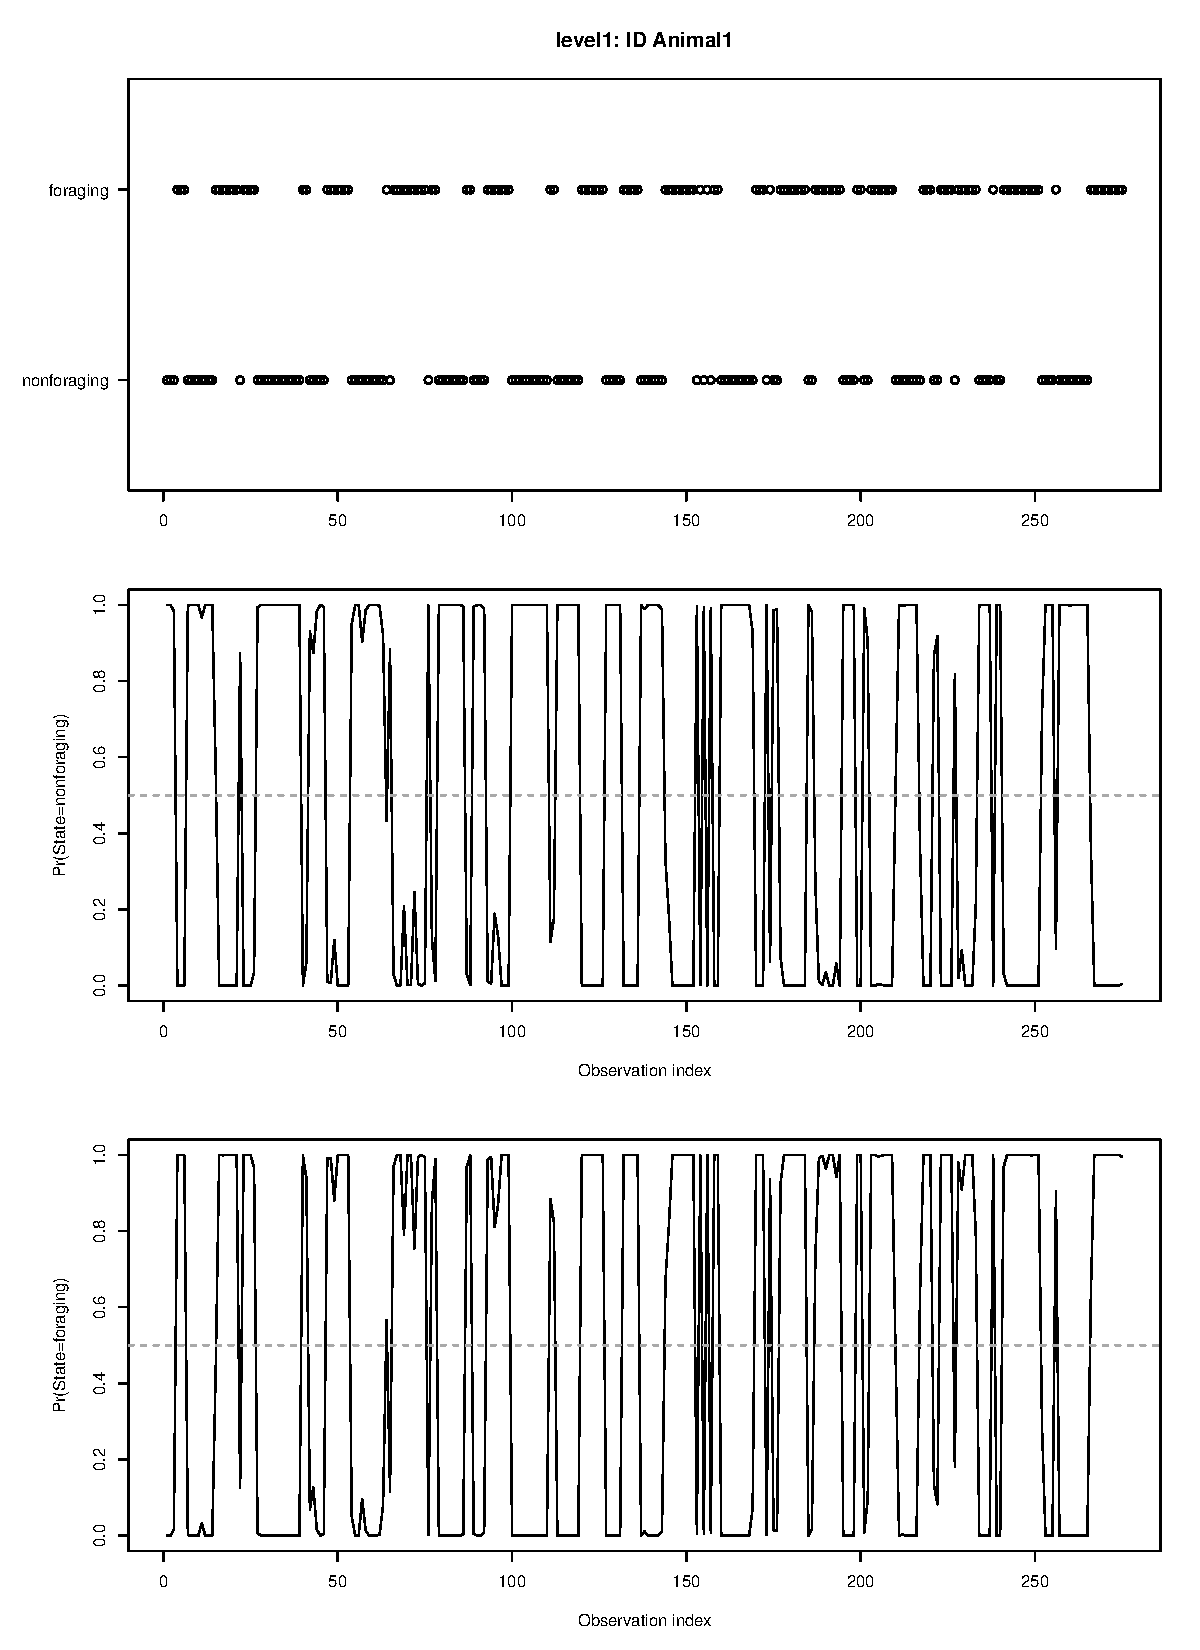
\includegraphics[width=\textwidth]{plot_harborPorpoiseStates001.pdf}
  \caption{Coarse-scale state probabilities for the harbor porpoise example.}
  \label{fig:hpLevel1}
\end{figure}
\begin{figure}[htbp]
  \centering
  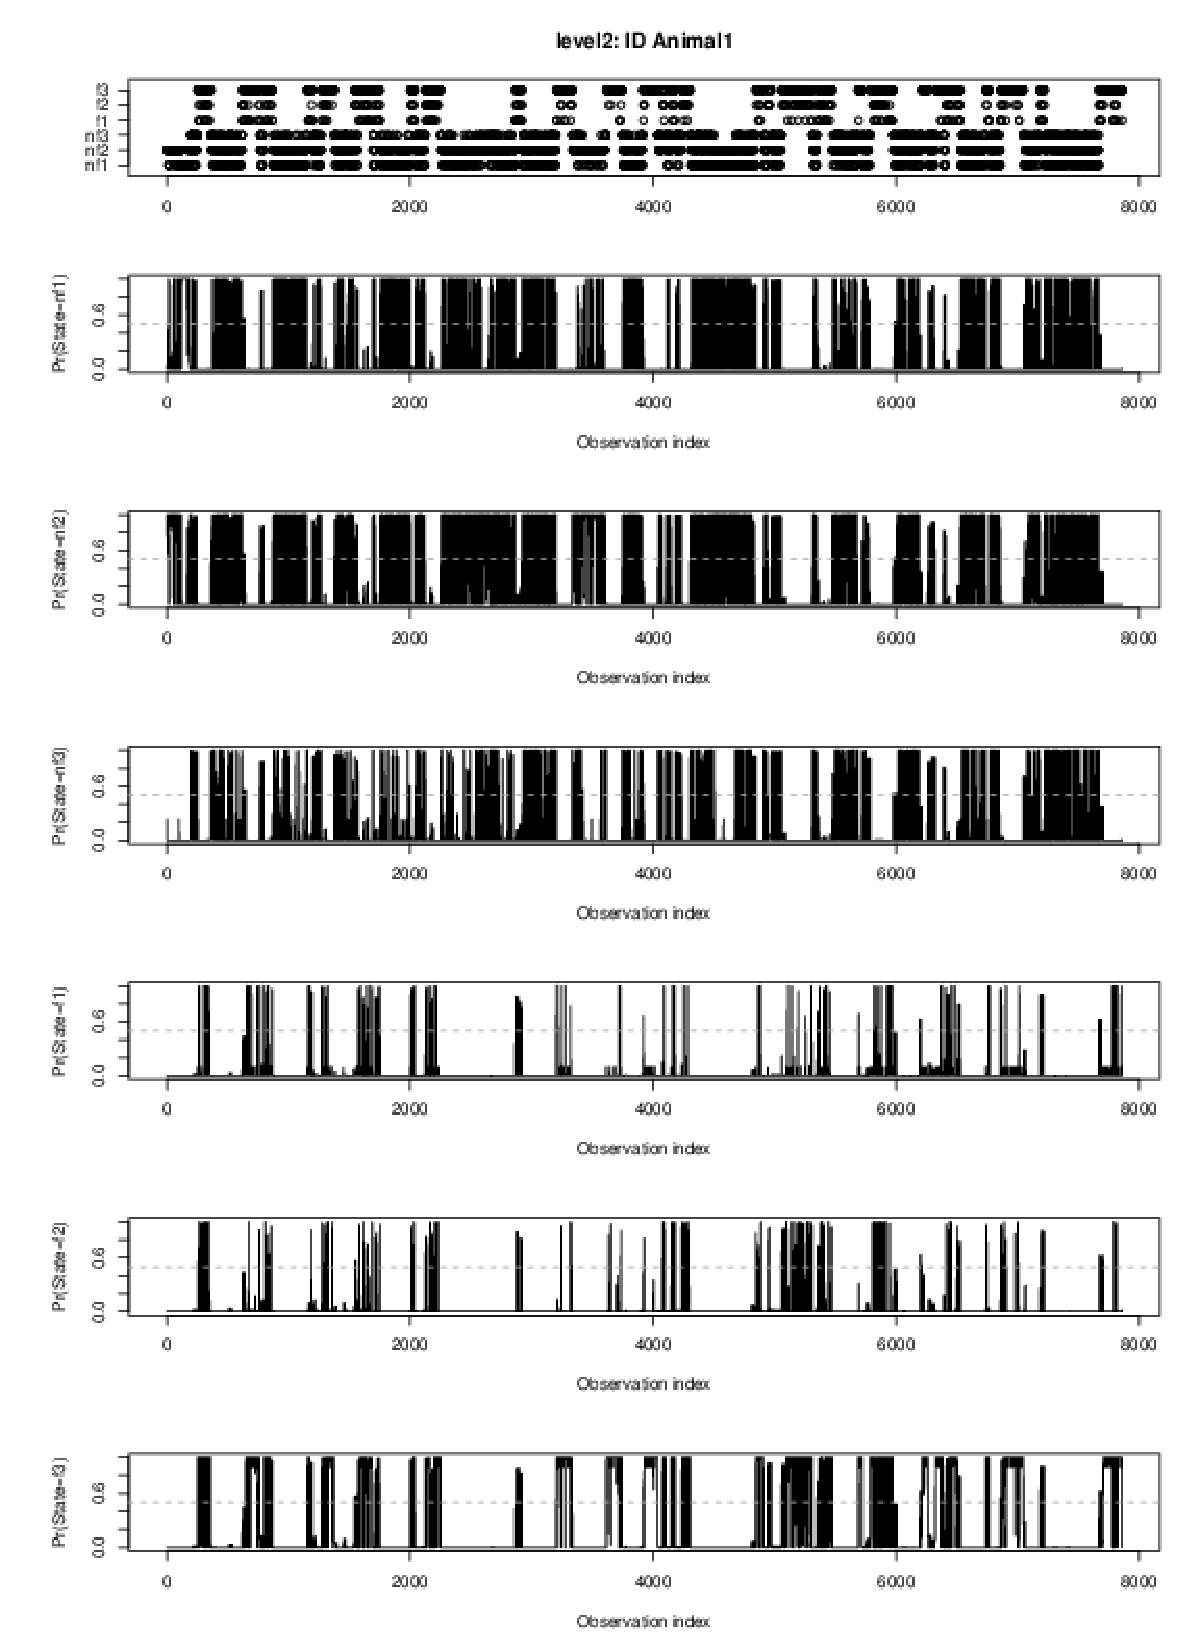
\includegraphics[width=\textwidth]{plot_harborPorpoiseStates002.pdf}
  \caption{Fine-scale state probabilities for the harbor porpoise example.}
  \label{fig:hpLevel2}
\end{figure}

We can also calculate the stationary probabilities of each state for each level of the hierarchy:
\begin{knitrout}
\definecolor{shadecolor}{rgb}{0.969, 0.969, 0.969}\color{fgcolor}\begin{kframe}
\begin{alltt}
\hlcom{# stationary distributions}
\hlstd{stats} \hlkwb{<-} \hlkwd{stationary}\hlstd{(hhmm)}

\hlcom{# coarse scale }
\hlstd{stats[[}\hlnum{1}\hlstd{]]}\hlopt{$}\hlstd{level1[}\hlnum{1}\hlstd{,]}
\end{alltt}
\begin{verbatim}
## nonforaging    foraging 
##   0.5026783   0.4973217
\end{verbatim}
\begin{alltt}
\hlcom{# fine scale }
\hlkwd{lapply}\hlstd{(stats[[}\hlnum{1}\hlstd{]]}\hlopt{$}\hlstd{level2,}\hlkwa{function}\hlstd{(}\hlkwc{x}\hlstd{) x[}\hlnum{1}\hlstd{,])}
\end{alltt}
\begin{verbatim}
## $nonforaging
##       nf1       nf2       nf3 
## 0.2793776 0.5060948 0.2145275 
## 
## $foraging
##         f1         f2         f3 
## 0.08308895 0.11164215 0.80526890
\end{verbatim}
\end{kframe}
\end{knitrout}

Finally, we can simulate from our fitted HHMM using the \verb|simHierData| function. This requires that we specify the number of observations for each level of the hierarchy as a \verb|data.tree| \verb|Node| (with attribute \verb|obs|) using the \verb|obsPerLevel| argument:
\begin{knitrout}
\definecolor{shadecolor}{rgb}{0.969, 0.969, 0.969}\color{fgcolor}\begin{kframe}
\begin{alltt}
\hlstd{obsPerLevel} \hlkwb{<-} \hlstd{data.tree}\hlopt{::}\hlstd{Node}\hlopt{$}\hlkwd{new}\hlstd{(}\hlstr{"simHierData"}\hlstd{)}

\hlcom{# number of level 1 observations}
\hlstd{obsPerLevel}\hlopt{$}\hlkwd{AddChild}\hlstd{(}\hlstr{"level1"}\hlstd{,}\hlkwc{obs}\hlstd{=}\hlnum{100}\hlstd{)}

\hlcom{# number of level 2 observations that follow each level 1 observation}
\hlstd{obsPerLevel}\hlopt{$}\hlkwd{AddChild}\hlstd{(}\hlstr{"level2"}\hlstd{,}\hlkwc{obs}\hlstd{=}\hlnum{25}\hlstd{)}

\hlstd{simHHMM} \hlkwb{<-} \hlkwd{simHierData}\hlstd{(}\hlkwc{model}\hlstd{=hhmm,}
                       \hlkwc{obsPerLevel} \hlstd{= obsPerLevel,} \hlkwc{states} \hlstd{=} \hlnum{TRUE}\hlstd{)}
\end{alltt}


{\ttfamily\noindent\itshape\color{messagecolor}{\#\# =======================================================================}}

{\ttfamily\noindent\itshape\color{messagecolor}{\#\# Simulating hierarchical HMM with 6 states and 3 data streams}}

{\ttfamily\noindent\itshape\color{messagecolor}{\#\# -----------------------------------------------------------------------}}

{\ttfamily\noindent\itshape\color{messagecolor}{\#\#\ \ dive\_duration \textasciitilde{} gamma(mean: custom, sd: custom)}}

{\ttfamily\noindent\itshape\color{messagecolor}{\#\#\ \ maximum\_depth \textasciitilde{} gamma(mean: custom, sd: custom)}}

{\ttfamily\noindent\itshape\color{messagecolor}{\#\#\ \ dive\_wiggliness \textasciitilde{} gamma(mean: custom, sd: custom, zeromass: custom)}}

{\ttfamily\noindent\itshape\color{messagecolor}{\#\# \\\#\#\ \ Transition probability matrix formula: \textasciitilde{}0 + I((level == "{}1"{}) * 1) + I((level == "{}2i"{}) * 1) + I((level == "{}2"{}) * 1)}}

{\ttfamily\noindent\itshape\color{messagecolor}{\#\# \\\#\#\ \ Initial distribution formula: \textasciitilde{}1}}

{\ttfamily\noindent\itshape\color{messagecolor}{\#\# =======================================================================}}

{\ttfamily\noindent\itshape\color{messagecolor}{\#\# DONE}}\begin{alltt}
\hlkwd{head}\hlstd{(simHHMM)}
\end{alltt}
\begin{verbatim}
##   ID level dive_duration maximum_depth dive_wiggliness states
## 1  1     1            NA            NA              NA      1
## 2  1    2i            NA            NA              NA      2
## 3  1     2      50.75401     19.444787      11.0461151      2
## 4  1     2      16.89706     16.166635      32.4377175      2
## 5  1     2      11.40743      4.024188       0.6959951      1
## 6  1     2      85.22059     35.200063      60.0786026      3
\end{verbatim}
\end{kframe}
\end{knitrout}

\subsubsection{Garter snakes}
\label{sec:garterSnake}
Next we'll quickly demonstrate how to perform the HHMM analysis for the garter snake movement data in \cite{Leos-BarajasEtAl2017} using \verb|momentuHMM|. This is also a 2-level HHMM, but now we include three coarse-scale states each composed of three fine-scale states (for a total of $N=9$ states).  As before, we must first add the \verb|level| field to our data to indicate the level of the hierarchy for each observation and then create a \verb|momentuHierHMMData| object with \verb|prepData|:
\begin{knitrout}
\definecolor{shadecolor}{rgb}{0.969, 0.969, 0.969}\color{fgcolor}\begin{kframe}
\begin{alltt}
\hlcom{# load garter snake data from Leos-Barajas et al}
\hlkwd{load}\hlstd{(}\hlkwd{url}\hlstd{(}\hlkwd{paste0}\hlstd{(}\hlstr{"https://static-content.springer.com/esm/"}\hlstd{,}
                \hlstr{"art%3A10.1007%2Fs13253-017-0282-9/MediaObjects/"}\hlstd{,}
                \hlstr{"13253_2017_282_MOESM1_ESM.rdata"}\hlstd{)))}

\hlstd{W} \hlkwb{<-} \hlkwd{dim}\hlstd{(dataAr)[}\hlnum{3}\hlstd{]} \hlcom{# number of individuals}
\hlstd{M} \hlkwb{<-} \hlkwd{dim}\hlstd{(dataAr)[}\hlnum{2}\hlstd{]} \hlcom{# number of time series per individual}

\hlcom{### add 2 extra rows for each time step where coarse scale behavior switches occur}
\hlcom{# level=1  indicates when coarse-scale behavior switching can occur }
\hlcom{# level=2i indicates start of each fine-scale interval}
\hlcom{# level=2  indicates when fine-scale behavior switching can occur}
\hlstd{snakeData} \hlkwb{<-} \hlkwa{NULL}
\hlkwa{for}\hlstd{(w} \hlkwa{in} \hlnum{1}\hlopt{:}\hlstd{W)\{}
  \hlstd{coarseInd} \hlkwb{<-} \hlkwd{data.frame}\hlstd{(}\hlkwc{ID}\hlstd{=w,}\hlkwc{level}\hlstd{=}\hlkwd{c}\hlstd{(}\hlstr{"1"}\hlstd{,}\hlstr{"2i"}\hlstd{),}\hlkwc{step}\hlstd{=}\hlnum{NA}\hlstd{)}
  \hlkwa{for}\hlstd{(m} \hlkwa{in} \hlnum{1}\hlopt{:}\hlstd{M)\{}
    \hlstd{tmp} \hlkwb{<-} \hlkwd{rbind}\hlstd{(coarseInd,}\hlkwd{data.frame}\hlstd{(}\hlkwc{ID}\hlstd{=w,}\hlkwc{level}\hlstd{=}\hlstr{"2"}\hlstd{,}\hlkwc{step}\hlstd{=}\hlkwd{sqrt}\hlstd{(dataAr[,m,w])))}
    \hlstd{snakeData} \hlkwb{<-} \hlkwd{rbind}\hlstd{(snakeData,tmp)}
  \hlstd{\}}
\hlstd{\}}

\hlcom{# prepare hierarchical data}
\hlstd{snakeData} \hlkwb{<-} \hlkwd{prepData}\hlstd{(snakeData,}\hlkwc{coordNames}\hlstd{=}\hlkwa{NULL}\hlstd{,}\hlkwc{hierLevels}\hlstd{=}\hlkwd{c}\hlstd{(}\hlstr{"1"}\hlstd{,}\hlstr{"2i"}\hlstd{,}\hlstr{"2"}\hlstd{))}

\hlcom{# summarize prepared data}
\hlkwd{summary}\hlstd{(snakeData)}
\end{alltt}
\begin{verbatim}
## Hierarchical HMM data for 19 individuals:
## 
## 1 -- 606 observations
## 2 -- 606 observations
## 3 -- 606 observations
## 4 -- 606 observations
## 5 -- 606 observations
## 6 -- 606 observations
## 7 -- 606 observations
## 8 -- 606 observations
## 9 -- 606 observations
## 10 -- 606 observations
## 11 -- 606 observations
## 12 -- 606 observations
## 13 -- 606 observations
## 14 -- 606 observations
## 15 -- 606 observations
## 16 -- 606 observations
## 17 -- 606 observations
## 18 -- 606 observations
## 19 -- 606 observations
## 
## 
## Data summaries:
## 
##       step       level     
##  Min.   :0.011   1 :  114  
##  1st Qu.:0.334   2i:  114  
##  Median :0.700   2 :11286  
##  Mean   :0.790             
##  3rd Qu.:1.149             
##  Max.   :3.130             
##  NA's   :1496
\end{verbatim}
\end{kframe}
\end{knitrout}
\noindent The sole data stream for this example is step length at the fine-scale level, and no coordinates are provided (hence \verb|coordNames=NULL|). As in section \ref{sec:harborPorpoise}, this example has no data streams observed at the coarse-scale level, but these could be easily included (if available; see sections \ref{sec:atlanticCod} and \ref{sec:hornShark}). Let's now specify the probability distribution for the fine-scale step length data stream via the \verb|hierDist| data tree Node:
\begin{knitrout}
\definecolor{shadecolor}{rgb}{0.969, 0.969, 0.969}\color{fgcolor}\begin{kframe}
\begin{alltt}
\hlcom{### data stream distributions: }
\hlcom{### level 1 = coarse level (no data streams)}
\hlcom{### level 2 = fine level (step="gamma")}
\hlstd{hierDist} \hlkwb{<-} \hlstd{data.tree}\hlopt{::}\hlstd{Node}\hlopt{$}\hlkwd{new}\hlstd{(}\hlstr{"garter snake HHMM dist"}\hlstd{)}
\hlstd{hierDist}\hlopt{$}\hlkwd{AddChild}\hlstd{(}\hlkwc{name}\hlstd{=}\hlstr{"level1"}\hlstd{)}
\hlstd{hierDist}\hlopt{$}\hlkwd{AddChild}\hlstd{(}\hlkwc{name}\hlstd{=}\hlstr{"level2"}\hlstd{)}
\hlstd{hierDist}\hlopt{$}\hlstd{level2}\hlopt{$}\hlkwd{AddChild}\hlstd{(}\hlkwc{name}\hlstd{=}\hlstr{"step"}\hlstd{,} \hlkwc{dist}\hlstd{=}\hlstr{"gamma"}\hlstd{)}

\hlkwd{plot}\hlstd{(hierDist)}
\end{alltt}
\end{kframe}
\includegraphics[width=\maxwidth]{figure/garterSnake-4-1} 

\end{knitrout}

Next we define our HHMM structure via the \verb|hierStates| data tree Node:
\begin{knitrout}
\definecolor{shadecolor}{rgb}{0.969, 0.969, 0.969}\color{fgcolor}\begin{kframe}
\begin{alltt}
\hlcom{### define hierarchical HMM: states 1-3 = coarse state 1}
\hlcom{###                          states 4-6 = coarse state 2}
\hlcom{###                          states 7-9 = coarse state 3}
\hlstd{hierStates} \hlkwb{<-} \hlstd{data.tree}\hlopt{::}\hlstd{Node}\hlopt{$}\hlkwd{new}\hlstd{(}\hlstr{"garter snake HHMM states"}\hlstd{)}
\hlstd{hierStates}\hlopt{$}\hlkwd{AddChild}\hlstd{(}\hlkwc{name}\hlstd{=}\hlstr{"internalState1"}\hlstd{)}
\hlstd{hierStates}\hlopt{$}\hlstd{internalState1}\hlopt{$}\hlkwd{AddChild}\hlstd{(}\hlkwc{name}\hlstd{=}\hlstr{"mo1"}\hlstd{,} \hlkwc{state}\hlstd{=}\hlnum{1}\hlstd{)} \hlcom{# motionless}
\hlstd{hierStates}\hlopt{$}\hlstd{internalState1}\hlopt{$}\hlkwd{AddChild}\hlstd{(}\hlkwc{name}\hlstd{=}\hlstr{"ex1"}\hlstd{,} \hlkwc{state}\hlstd{=}\hlnum{2}\hlstd{)} \hlcom{# slow exploratory}
\hlstd{hierStates}\hlopt{$}\hlstd{internalState1}\hlopt{$}\hlkwd{AddChild}\hlstd{(}\hlkwc{name}\hlstd{=}\hlstr{"es1"}\hlstd{,} \hlkwc{state}\hlstd{=}\hlnum{3}\hlstd{)} \hlcom{# rapid escape}
\hlstd{hierStates}\hlopt{$}\hlkwd{AddChild}\hlstd{(}\hlkwc{name}\hlstd{=}\hlstr{"internalState2"}\hlstd{)}
\hlstd{hierStates}\hlopt{$}\hlstd{internalState2}\hlopt{$}\hlkwd{AddChild}\hlstd{(}\hlkwc{name}\hlstd{=}\hlstr{"mo2"}\hlstd{,} \hlkwc{state}\hlstd{=}\hlnum{4}\hlstd{)} \hlcom{# motionless}
\hlstd{hierStates}\hlopt{$}\hlstd{internalState2}\hlopt{$}\hlkwd{AddChild}\hlstd{(}\hlkwc{name}\hlstd{=}\hlstr{"ex2"}\hlstd{,} \hlkwc{state}\hlstd{=}\hlnum{5}\hlstd{)} \hlcom{# slow exploratory}
\hlstd{hierStates}\hlopt{$}\hlstd{internalState2}\hlopt{$}\hlkwd{AddChild}\hlstd{(}\hlkwc{name}\hlstd{=}\hlstr{"es2"}\hlstd{,} \hlkwc{state}\hlstd{=}\hlnum{6}\hlstd{)} \hlcom{# rapid escape}
\hlstd{hierStates}\hlopt{$}\hlkwd{AddChild}\hlstd{(}\hlkwc{name}\hlstd{=}\hlstr{"internalState3"}\hlstd{)}
\hlstd{hierStates}\hlopt{$}\hlstd{internalState3}\hlopt{$}\hlkwd{AddChild}\hlstd{(}\hlkwc{name}\hlstd{=}\hlstr{"mo3"}\hlstd{,} \hlkwc{state}\hlstd{=}\hlnum{7}\hlstd{)} \hlcom{# motionless}
\hlstd{hierStates}\hlopt{$}\hlstd{internalState3}\hlopt{$}\hlkwd{AddChild}\hlstd{(}\hlkwc{name}\hlstd{=}\hlstr{"ex3"}\hlstd{,} \hlkwc{state}\hlstd{=}\hlnum{8}\hlstd{)} \hlcom{# slow exploratory}
\hlstd{hierStates}\hlopt{$}\hlstd{internalState3}\hlopt{$}\hlkwd{AddChild}\hlstd{(}\hlkwc{name}\hlstd{=}\hlstr{"es3"}\hlstd{,} \hlkwc{state}\hlstd{=}\hlnum{9}\hlstd{)} \hlcom{# rapid escape}
\end{alltt}
\end{kframe}
\end{knitrout}
\noindent Or, equivalently: 
\begin{knitrout}
\definecolor{shadecolor}{rgb}{0.969, 0.969, 0.969}\color{fgcolor}\begin{kframe}
\begin{alltt}
\hlstd{hierStates} \hlkwb{<-} \hlstd{data.tree}\hlopt{::}\hlkwd{as.Node}\hlstd{(}\hlkwd{list}\hlstd{(}\hlkwc{name}\hlstd{=}\hlstr{"garter snake HHMM states"}\hlstd{,}
                                      \hlkwc{internalState1}\hlstd{=}\hlkwd{list}\hlstd{(}\hlkwc{mo1}\hlstd{=}\hlkwd{list}\hlstd{(}\hlkwc{state}\hlstd{=}\hlnum{1}\hlstd{),}
                                                          \hlkwc{ex1}\hlstd{=}\hlkwd{list}\hlstd{(}\hlkwc{state}\hlstd{=}\hlnum{2}\hlstd{),}
                                                          \hlkwc{es1}\hlstd{=}\hlkwd{list}\hlstd{(}\hlkwc{state}\hlstd{=}\hlnum{3}\hlstd{)),}
                                      \hlkwc{internalState2}\hlstd{=}\hlkwd{list}\hlstd{(}\hlkwc{mo2}\hlstd{=}\hlkwd{list}\hlstd{(}\hlkwc{state}\hlstd{=}\hlnum{4}\hlstd{),}
                                                          \hlkwc{ex2}\hlstd{=}\hlkwd{list}\hlstd{(}\hlkwc{state}\hlstd{=}\hlnum{5}\hlstd{),}
                                                          \hlkwc{es2}\hlstd{=}\hlkwd{list}\hlstd{(}\hlkwc{state}\hlstd{=}\hlnum{6}\hlstd{)),}
                                      \hlkwc{internalState3}\hlstd{=}\hlkwd{list}\hlstd{(}\hlkwc{mo3}\hlstd{=}\hlkwd{list}\hlstd{(}\hlkwc{state}\hlstd{=}\hlnum{7}\hlstd{),}
                                                          \hlkwc{ex3}\hlstd{=}\hlkwd{list}\hlstd{(}\hlkwc{state}\hlstd{=}\hlnum{8}\hlstd{),}
                                                          \hlkwc{es3}\hlstd{=}\hlkwd{list}\hlstd{(}\hlkwc{state}\hlstd{=}\hlnum{9}\hlstd{))))}
\hlkwd{plot}\hlstd{(hierStates)}
\end{alltt}
\end{kframe}
\includegraphics[width=\maxwidth]{figure/garterSnake-3-1} 

\end{knitrout}

As in the harbor porpoise example (section \ref{sec:harborPorpoise}), we follow \cite{Leos-BarajasEtAl2017} and assume the fine-scale data stream probability distribution does not depend on coarse-scale state:
\begin{knitrout}
\definecolor{shadecolor}{rgb}{0.969, 0.969, 0.969}\color{fgcolor}\begin{kframe}
\begin{alltt}
\hlcom{# defining start values for step data stream}
\hlstd{mu0} \hlkwb{<-} \hlkwd{c}\hlstd{(}\hlnum{0.121}\hlstd{,}\hlnum{0.678}\hlstd{,}\hlnum{1.375}\hlstd{)}
\hlstd{sd0} \hlkwb{<-} \hlkwd{c}\hlstd{(}\hlnum{0.06}\hlstd{,}\hlnum{0.321}\hlstd{,}\hlnum{0.4875}\hlstd{)}
\hlstd{Par0} \hlkwb{<-} \hlkwd{list}\hlstd{(}\hlkwc{step}\hlstd{=}\hlkwd{c}\hlstd{(}\hlkwd{rep}\hlstd{(mu0,hierStates}\hlopt{$}\hlstd{count),}\hlkwd{rep}\hlstd{(sd0,hierStates}\hlopt{$}\hlstd{count)))}

\hlstd{nbStates} \hlkwb{<-} \hlkwd{length}\hlstd{(hierStates}\hlopt{$}\hlkwd{Get}\hlstd{(}\hlstr{"state"}\hlstd{,}\hlkwc{filterFun}\hlstd{=data.tree}\hlopt{::}\hlstd{isLeaf))}

\hlcom{# constrain data stream distributions to be same for coarse-scale states}
\hlstd{DM} \hlkwb{<-} \hlkwd{list}\hlstd{(}\hlkwc{step}\hlstd{=}\hlkwd{matrix}\hlstd{(}\hlkwd{cbind}\hlstd{(}\hlkwd{kronecker}\hlstd{(}\hlkwd{c}\hlstd{(}\hlnum{1}\hlstd{,}\hlnum{1}\hlstd{,}\hlnum{1}\hlstd{,}\hlnum{0}\hlstd{,}\hlnum{0}\hlstd{,}\hlnum{0}\hlstd{),}\hlkwd{diag}\hlstd{(}\hlnum{3}\hlstd{)),}
                             \hlkwd{kronecker}\hlstd{(}\hlkwd{c}\hlstd{(}\hlnum{0}\hlstd{,}\hlnum{0}\hlstd{,}\hlnum{0}\hlstd{,}\hlnum{1}\hlstd{,}\hlnum{1}\hlstd{,}\hlnum{1}\hlstd{),}\hlkwd{diag}\hlstd{(}\hlnum{3}\hlstd{))),}
                       \hlkwc{nrow}\hlstd{=nbStates}\hlopt{*}\hlnum{2}\hlstd{,}
                       \hlkwc{ncol}\hlstd{=}\hlnum{6}\hlstd{,}
                       \hlkwc{dimnames}\hlstd{=}\hlkwd{list}\hlstd{(}\hlkwd{c}\hlstd{(}\hlkwd{paste0}\hlstd{(}\hlstr{"mean_"}\hlstd{,}\hlnum{1}\hlopt{:}\hlstd{nbStates),}
                                       \hlkwd{paste0}\hlstd{(}\hlstr{"sd_"}\hlstd{,}\hlnum{1}\hlopt{:}\hlstd{nbStates)),}
                                     \hlkwd{paste0}\hlstd{(}\hlkwd{rep}\hlstd{(}\hlkwd{c}\hlstd{(}\hlstr{"mean"}\hlstd{,}\hlstr{"sd"}\hlstd{),}\hlkwc{each}\hlstd{=}\hlnum{3}\hlstd{),}
                                            \hlkwd{c}\hlstd{(}\hlstr{"_147:(Intercept)"}\hlstd{,}
                                              \hlstr{"_258:(Intercept)"}\hlstd{,}
                                              \hlstr{"_369:(Intercept)"}\hlstd{)))))}

\hlcom{# initial parameter values for data stream probability distributions}
\hlstd{Par} \hlkwb{<-} \hlkwd{getParDM}\hlstd{(snakeData,}
                \hlkwc{hierStates}\hlstd{=hierStates,}\hlkwc{hierDist}\hlstd{=hierDist,}
                \hlkwc{Par}\hlstd{=Par0,}\hlkwc{DM}\hlstd{=DM)}
\end{alltt}
\end{kframe}
\end{knitrout}

We do not include any covariates in \verb|hierFormula| or \verb|hierFormulaDelta|, so all that's left before fitting the model is the (optional) step of specifying starting values for the t.p.m. and initial distribution at each level of the hierarchy \citep[based on values reported by][]{Leos-BarajasEtAl2017}:
\begin{knitrout}
\definecolor{shadecolor}{rgb}{0.969, 0.969, 0.969}\color{fgcolor}\begin{kframe}
\begin{alltt}
\hlstd{hierBeta} \hlkwb{<-} \hlstd{data.tree}\hlopt{::}\hlstd{Node}\hlopt{$}\hlkwd{new}\hlstd{(}\hlstr{"garter snake beta"}\hlstd{)}
\hlstd{hierBeta}\hlopt{$}\hlkwd{AddChild}\hlstd{(}\hlkwc{name}\hlstd{=}\hlstr{"level1"}\hlstd{)}
\hlstd{hierBeta}\hlopt{$}\hlkwd{AddChild}\hlstd{(}\hlkwc{name}\hlstd{=}\hlstr{"level2"}\hlstd{)}
\hlstd{hierBeta}\hlopt{$}\hlstd{level2}\hlopt{$}\hlkwd{AddChild}\hlstd{(}\hlkwc{name}\hlstd{=}\hlstr{"internalState1"}\hlstd{)}
\hlstd{hierBeta}\hlopt{$}\hlstd{level2}\hlopt{$}\hlkwd{AddChild}\hlstd{(}\hlkwc{name}\hlstd{=}\hlstr{"internalState2"}\hlstd{)}
\hlstd{hierBeta}\hlopt{$}\hlstd{level2}\hlopt{$}\hlkwd{AddChild}\hlstd{(}\hlkwc{name}\hlstd{=}\hlstr{"internalState3"}\hlstd{)}

\hlstd{hierDelta} \hlkwb{<-} \hlstd{data.tree}\hlopt{::}\hlkwd{Clone}\hlstd{(hierBeta)}
\hlstd{hierDelta}\hlopt{$}\hlstd{name} \hlkwb{<-} \hlstr{"garter snake delta"}

\hlcom{# reference states for level1}
\hlstd{level1states} \hlkwb{<-} \hlstd{hierStates}\hlopt{$}\hlkwd{Get}\hlstd{(}\hlkwa{function}\hlstd{(}\hlkwc{x}\hlstd{) data.tree}\hlopt{::}\hlkwd{Aggregate}\hlstd{(x,}\hlstr{"state"}\hlstd{,min),}
                               \hlkwc{filterFun}\hlstd{=}\hlkwa{function}\hlstd{(}\hlkwc{x}\hlstd{) x}\hlopt{$}\hlstd{level}\hlopt{==}\hlnum{2}\hlstd{)}

\hlstd{hierBeta}\hlopt{$}\hlstd{level1}\hlopt{$}\hlstd{beta} \hlkwb{<-} \hlkwd{matrix}\hlstd{(}\hlkwd{c}\hlstd{(}\hlnum{1.24}\hlstd{,} \hlnum{0.44}\hlstd{,} \hlnum{1.1}\hlstd{,} \hlopt{-}\hlnum{0.87}\hlstd{,} \hlopt{-}\hlnum{1.40}\hlstd{,} \hlopt{-}\hlnum{1.11}\hlstd{),}
                               \hlkwc{nrow}\hlstd{=}\hlnum{1}\hlstd{,}
                               \hlkwc{ncol}\hlstd{=hierStates}\hlopt{$}\hlstd{count}\hlopt{*}\hlstd{(hierStates}\hlopt{$}\hlstd{count}\hlopt{-}\hlnum{1}\hlstd{),}
                               \hlkwc{byrow}\hlstd{=}\hlnum{TRUE}\hlstd{,}
                               \hlkwc{dimnames}\hlstd{=}\hlkwd{list}\hlstd{(}\hlstr{"(Intercept)"}\hlstd{,}
                                        \hlkwd{c}\hlstd{(}\hlkwd{sapply}\hlstd{(level1states,}\hlkwa{function}\hlstd{(}\hlkwc{x}\hlstd{)}
                                          \hlkwd{paste}\hlstd{(}
                                           \hlkwd{rep}\hlstd{(x,}\hlkwc{each}\hlstd{=hierStates}\hlopt{$}\hlstd{count}\hlopt{-}\hlnum{1}\hlstd{),}
                                           \hlstr{"->"}\hlstd{,}
                                           \hlstd{level1states[}\hlopt{-}\hlkwd{which}\hlstd{(level1states}\hlopt{==}\hlstd{x)])))))}

\hlstd{hierDelta}\hlopt{$}\hlstd{level1}\hlopt{$}\hlstd{delta} \hlkwb{<-} \hlkwd{matrix}\hlstd{(}\hlkwd{rep}\hlstd{(}\hlkwd{c}\hlstd{(}\hlopt{-}\hlnum{2.5}\hlstd{,}\hlopt{-}\hlnum{3.5}\hlstd{),hierStates}\hlopt{$}\hlstd{count}\hlopt{-}\hlnum{1}\hlstd{),}
                                 \hlkwc{nrow}\hlstd{=}\hlnum{1}\hlstd{,}
                                 \hlkwc{ncol}\hlstd{=(hierStates}\hlopt{$}\hlstd{count}\hlopt{-}\hlnum{1}\hlstd{),}
                                 \hlkwc{byrow}\hlstd{=}\hlnum{TRUE}\hlstd{,}
                                 \hlkwc{dimnames}\hlstd{=}\hlkwd{list}\hlstd{(}\hlstr{"(Intercept)"}\hlstd{,}
                                               \hlkwd{paste}\hlstd{(}\hlstr{"state"}\hlstd{,level1states[}\hlopt{-}\hlnum{1}\hlstd{])))}

\hlstd{beta0_level2} \hlkwb{<-} \hlstd{delta0_level2} \hlkwb{<-} \hlkwd{list}\hlstd{()}
\hlstd{beta0_level2}\hlopt{$}\hlstd{internalState1} \hlkwb{<-} \hlkwd{c}\hlstd{(}\hlopt{-}\hlnum{2.99}\hlstd{,} \hlopt{-}\hlnum{5.06}\hlstd{,} \hlnum{3.93}\hlstd{,} \hlnum{1.25}\hlstd{,} \hlnum{34.84}\hlstd{,} \hlnum{35.97}\hlstd{)}
\hlstd{beta0_level2}\hlopt{$}\hlstd{internalState2} \hlkwb{<-} \hlkwd{c}\hlstd{(}\hlopt{-}\hlnum{1.72}\hlstd{,} \hlopt{-}\hlnum{2.78}\hlstd{,} \hlnum{3.54}\hlstd{,} \hlnum{2.83}\hlstd{,} \hlnum{34.72}\hlstd{,} \hlnum{36.21}\hlstd{)}
\hlstd{beta0_level2}\hlopt{$}\hlstd{internalState3} \hlkwb{<-} \hlkwd{c}\hlstd{(}\hlopt{-}\hlnum{5.10}\hlstd{,} \hlopt{-}\hlnum{17.69}\hlstd{,} \hlnum{5.76}\hlstd{,} \hlopt{-}\hlnum{11.34}\hlstd{,} \hlnum{33.39}\hlstd{,} \hlnum{37.37}\hlstd{)}

\hlstd{delta0_level2}\hlopt{$}\hlstd{internalState1} \hlkwb{<-} \hlkwd{c}\hlstd{(}\hlopt{-}\hlnum{1.39}\hlstd{,} \hlnum{0.16}\hlstd{)}
\hlstd{delta0_level2}\hlopt{$}\hlstd{internalState2} \hlkwb{<-} \hlkwd{c}\hlstd{(}\hlopt{-}\hlnum{1.27}\hlstd{,} \hlnum{2.33}\hlstd{)}
\hlstd{delta0_level2}\hlopt{$}\hlstd{internalState3} \hlkwb{<-} \hlkwd{c}\hlstd{(}\hlnum{0.34}\hlstd{,} \hlopt{-}\hlnum{0.26}\hlstd{)}

\hlkwa{for}\hlstd{(jj} \hlkwa{in} \hlnum{1}\hlopt{:}\hlstd{hierStates}\hlopt{$}\hlstd{count)\{}
  \hlstd{j} \hlkwb{<-}  \hlkwd{names}\hlstd{(hierStates}\hlopt{$}\hlstd{children)[jj]}

  \hlcom{# reference states for internalState j}
  \hlstd{ref} \hlkwb{<-} \hlstd{hierStates[[j]]}\hlopt{$}\hlkwd{Get}\hlstd{(}\hlkwa{function}\hlstd{(}\hlkwc{x}\hlstd{)}
                              \hlstd{data.tree}\hlopt{::}\hlkwd{Aggregate}\hlstd{(x,}\hlstr{"state"}\hlstd{,min),}
                             \hlkwc{filterFun}\hlstd{=}\hlkwa{function}\hlstd{(}\hlkwc{x}\hlstd{) x}\hlopt{$}\hlstd{level}\hlopt{==}\hlnum{2}\hlstd{)}

  \hlcom{# states for internalState j}
  \hlstd{states} \hlkwb{<-} \hlstd{hierStates[[j]]}\hlopt{$}\hlkwd{Get}\hlstd{(}\hlstr{"state"}\hlstd{,}\hlkwc{filterFun} \hlstd{= isLeaf)}

  \hlstd{dimNames} \hlkwb{<-} \hlkwd{list}\hlstd{(}\hlstr{"(Intercept)"}\hlstd{,}
                   \hlkwd{paste0}\hlstd{(}\hlkwd{rep}\hlstd{(states,}\hlkwc{each}\hlstd{=hierStates[[j]]}\hlopt{$}\hlstd{count}\hlopt{-}\hlnum{1}\hlstd{),}
                          \hlstr{" -> "}\hlstd{,}
                          \hlstd{states[}\hlopt{-}\hlkwd{which}\hlstd{(states}\hlopt{==}\hlstd{ref)]))}

  \hlstd{hierBeta}\hlopt{$}\hlstd{level2[[j]]}\hlopt{$}\hlstd{beta} \hlkwb{<-} \hlkwd{matrix}\hlstd{(beta0_level2[[j]],}
                                      \hlkwc{nrow}\hlstd{=}\hlnum{1}\hlstd{,}
                                      \hlkwc{ncol}\hlstd{=hierStates[[j]]}\hlopt{$}\hlstd{count}\hlopt{*}
                                           \hlstd{(hierStates[[j]]}\hlopt{$}\hlstd{count}\hlopt{-}\hlnum{1}\hlstd{),}
                                      \hlkwc{byrow}\hlstd{=}\hlnum{TRUE}\hlstd{,}
                                      \hlkwc{dimnames}\hlstd{=dimNames)}

  \hlstd{hierDelta}\hlopt{$}\hlstd{level2[[j]]}\hlopt{$}\hlstd{delta} \hlkwb{<-} \hlkwd{matrix}\hlstd{(delta0_level2[[j]],}
                                        \hlkwc{nrow}\hlstd{=}\hlnum{1}\hlstd{,}
                                        \hlkwc{ncol}\hlstd{=(hierStates[[j]]}\hlopt{$}\hlstd{count}\hlopt{-}\hlnum{1}\hlstd{),}
                                        \hlkwc{byrow}\hlstd{=}\hlnum{TRUE}\hlstd{,}
                                        \hlkwc{dimnames}\hlstd{=}\hlkwd{list}\hlstd{(}\hlstr{"(Intercept)"}\hlstd{,}
                                                      \hlkwd{names}\hlstd{(states)[}\hlopt{-}\hlnum{1}\hlstd{]))}
\hlstd{\}}
\end{alltt}
\end{kframe}
\end{knitrout}

Let's check our model specification:
\begin{knitrout}
\definecolor{shadecolor}{rgb}{0.969, 0.969, 0.969}\color{fgcolor}\begin{kframe}
\begin{alltt}
\hlkwd{checkPar0}\hlstd{(snakeData,}\hlkwc{hierStates}\hlstd{=hierStates,}\hlkwc{hierDist}\hlstd{=hierDist,}
          \hlkwc{Par0}\hlstd{=Par,}\hlkwc{DM}\hlstd{=DM,}
          \hlkwc{hierBeta}\hlstd{=hierBeta,}\hlkwc{hierDelta}\hlstd{=hierDelta)}
\end{alltt}
\begin{verbatim}
## 
## Regression coeffs for step parameters:
## --------------------------------------
##      mean_147:(Intercept) mean_258:(Intercept) mean_369:(Intercept)
## [1,]            -2.111965            -0.388608            0.3184537
##      sd_147:(Intercept) sd_258:(Intercept) sd_369:(Intercept)
## [1,]          -2.813411          -1.136314          -0.718465
## 
## ----------------------------------------------------------
## Regression coeffs for the transition probabilities (beta):
## ----------------------------------------------------------
## -------------------------  level1  -----------------------
##                       1 -> 4 1 -> 7 4 -> 1 4 -> 7 7 -> 1 7 -> 4
## I((level == "1") * 1)   1.24   0.44    1.1  -0.87   -1.4  -1.11
## 
## -------------------------  level2  -----------------------
##                       1 -> 2 1 -> 3 2 -> 2 2 -> 3 3 -> 2 3 -> 3
## I((level == "2") * 1)  -2.99  -5.06   3.93   1.25  34.84  35.97
## 
##                       4 -> 5 4 -> 6 5 -> 5 5 -> 6 6 -> 5 6 -> 6
## I((level == "2") * 1)  -1.72  -2.78   3.54   2.83  34.72  36.21
## 
##                       7 -> 8 7 -> 9 8 -> 8 8 -> 9 9 -> 8 9 -> 9
## I((level == "2") * 1)   -5.1 -17.69   5.76 -11.34  33.39  37.37
## 
## ----------------------------------------------------------
## 
## ----------------------------------------------------------
## Regression coeffs for the initial distribution (delta):
## ----------------------------------------------------------
## ------------------------  level1  ------------------------
##             state 4 state 7
## (Intercept)    -2.5    -3.5
## 
## ------------------------  level2  ------------------------
##                        state 2 state 3
## I((level == "2i") * 1)   -1.39    0.16
## 
##                        state 5 state 6
## I((level == "2i") * 1)   -1.27    2.33
## 
##                        state 8 state 9
## I((level == "2i") * 1)    0.34   -0.26
## 
## ----------------------------------------------------------
\end{verbatim}
\end{kframe}
\end{knitrout}
\noindent Again note that higher-level (i.e. ``parent'') states are indexed based on the lowest state index of their ``children''.  For example, ``internalState1'' is indexed by state 1, ``internalState2'' is indexed by state 4, and ``internalState3'' is indexed by state 7. We can also examine the starting values for the t.p.m. on the real scale (``\verb|gamma|'') at each level of the hierarchy using the \verb|getTrProbs| function:
\begin{knitrout}
\definecolor{shadecolor}{rgb}{0.969, 0.969, 0.969}\color{fgcolor}\begin{kframe}
\begin{alltt}
\hlstd{iTrProbs} \hlkwb{<-} \hlkwd{getTrProbs}\hlstd{(snakeData,}\hlkwc{hierStates}\hlstd{=hierStates,}
                       \hlkwc{hierBeta}\hlstd{=hierBeta,}\hlkwc{hierDist}\hlstd{=hierDist)}

\hlcom{# t.p.m. at first time step for level1}
\hlstd{iTrProbs}\hlopt{$}\hlstd{level1}\hlopt{$}\hlstd{gamma[,,}\hlnum{1}\hlstd{]}
\end{alltt}
\begin{verbatim}
##                internalState1 internalState2 internalState3
## internalState1      0.1664359      0.5751380     0.25842616
## internalState2      0.6791965      0.2260849     0.09471861
## internalState3      0.1564547      0.2090903     0.63445500
\end{verbatim}
\begin{alltt}
\hlcom{# t.p.m. at first time step for level2}
\hlkwd{lapply}\hlstd{(iTrProbs}\hlopt{$}\hlstd{level2,}\hlkwa{function}\hlstd{(}\hlkwc{x}\hlstd{) x}\hlopt{$}\hlstd{gamma[,,}\hlnum{1}\hlstd{])}
\end{alltt}
\begin{verbatim}
## $internalState1
##              mo1        ex1         es1
## mo1 9.464024e-01 0.04759215 0.006005453
## ex1 1.805141e-02 0.91894296 0.063005628
## es1 1.806578e-16 0.24416110 0.755838899
## 
## $internalState2
##              mo2       ex2        es2
## mo2 8.057338e-01 0.1442797 0.04998652
## ex2 1.907946e-02 0.6576103 0.32331027
## es2 1.534365e-16 0.1839217 0.81607827
## 
## $internalState3
##              mo3         ex3          es3
## mo3 9.939402e-01 0.006059801 2.063911e-08
## ex3 3.141213e-03 0.996858749 3.734204e-08
## es3 5.785955e-17 0.018342891 9.816571e-01
\end{verbatim}
\end{kframe}
\end{knitrout}

Now let's fit our garter snake HHMM:
\begin{knitrout}
\definecolor{shadecolor}{rgb}{0.969, 0.969, 0.969}\color{fgcolor}\begin{kframe}
\begin{alltt}
\hlcom{# fit hierarchical HMM}
\hlstd{hhmm} \hlkwb{<-} \hlkwd{fitHMM}\hlstd{(snakeData,}\hlkwc{hierStates}\hlstd{=hierStates,}\hlkwc{hierDist}\hlstd{=hierDist,}
               \hlkwc{Par0}\hlstd{=Par,}\hlkwc{DM}\hlstd{=DM,}\hlkwc{hierBeta}\hlstd{=hierBeta,}\hlkwc{hierDelta}\hlstd{=hierDelta,}
               \hlkwc{nlmPar}\hlstd{=}\hlkwd{list}\hlstd{(}\hlkwc{hessian}\hlstd{=}\hlnum{FALSE}\hlstd{))}
\end{alltt}


{\ttfamily\noindent\itshape\color{messagecolor}{\#\# =======================================================================}}

{\ttfamily\noindent\itshape\color{messagecolor}{\#\# Fitting hierarchical HMM with 9 states and 1 data stream}}

{\ttfamily\noindent\itshape\color{messagecolor}{\#\# -----------------------------------------------------------------------}}

{\ttfamily\noindent\itshape\color{messagecolor}{\#\#\ \ step \textasciitilde{} gamma(mean: custom, sd: custom)}}

{\ttfamily\noindent\itshape\color{messagecolor}{\#\# \\\#\#\ \ Transition probability matrix formula: \textasciitilde{}0 + I((level == "{}1"{}) * 1) + I((level == "{}2i"{}) * 1) + I((level == "{}2"{}) * 1)}}

{\ttfamily\noindent\itshape\color{messagecolor}{\#\# \\\#\#\ \ Initial distribution formula: \textasciitilde{}1}}

{\ttfamily\noindent\itshape\color{messagecolor}{\#\# =======================================================================}}

{\ttfamily\noindent\itshape\color{messagecolor}{\#\# DONE}}\end{kframe}
\end{knitrout}
\begin{knitrout}
\definecolor{shadecolor}{rgb}{0.969, 0.969, 0.969}\color{fgcolor}\begin{kframe}
\begin{alltt}
\hlstd{hhmm}
\end{alltt}
\begin{verbatim}
## Value of the maximum log-likelihood: -2060.361 
## 
## 
## step parameters:
## ----------------
##             mo1       ex1       es1        mo2       ex2       es2
## mean 0.12148244 0.6778589 1.3749453 0.12148244 0.6778589 1.3749453
## sd   0.05906919 0.3217373 0.4876126 0.05906919 0.3217373 0.4876126
##             mo3       ex3       es3
## mean 0.12148244 0.6778589 1.3749453
## sd   0.05906919 0.3217373 0.4876126
## 
## 
## ---------------------------------------------------------------
## Regression coeffs for the transition probabilities:
## ---------------------------------------------------------------
## --------------------------  level1  ---------------------------
##                         1 -> 4    1 -> 7   4 -> 1    4 -> 7    7 -> 1
## I((level == "1") * 1) 1.245638 0.4309528 1.102461 -0.870203 -1.397521
##                          7 -> 4
## I((level == "1") * 1) -1.114278
## 
## --------------------------  level2  ---------------------------
##                          1 -> 2    1 -> 3   2 -> 2   2 -> 3   3 -> 2
## I((level == "2") * 1) -2.993152 -5.064987 3.927787 1.246237 34.83412
##                         3 -> 3
## I((level == "2") * 1) 35.96589
## 
##                          4 -> 5    4 -> 6   5 -> 5   5 -> 6  6 -> 5
## I((level == "2") * 1) -1.721131 -2.775771 3.540737 2.834405 34.7087
##                         6 -> 6
## I((level == "2") * 1) 36.19201
## 
##                          7 -> 8    7 -> 9   8 -> 8    8 -> 9   9 -> 8
## I((level == "2") * 1) -5.098125 -17.69051 5.761101 -11.34101 33.38974
##                         9 -> 9
## I((level == "2") * 1) 37.36932
## 
## ---------------------------------------------------------------
## 
## ---------------------------------------------------------------
## Transition probability matrix (based on mean covariate values):
## ---------------------------------------------------------------
## --------------------------  level1  ---------------------------
##                internalState1 internalState2 internalState3
## internalState1      0.1662821      0.5778557     0.25586212
## internalState2      0.6797456      0.2257114     0.09454295
## internalState3      0.1569221      0.2083028     0.63477506
## 
## --------------------------  level2  ---------------------------
##              mo1        ex1         es1
## mo1 9.465724e-01 0.04745091 0.005976649
## ex1 1.809245e-02 0.91899585 0.062911698
## es1 1.814804e-16 0.24383417 0.756165834
## 
##              mo2       ex2        es2
## mo2 8.056946e-01 0.1441095 0.05019591
## ex2 1.904305e-02 0.6568391 0.32411785
## es2 1.560287e-16 0.1849270 0.81507302
## 
##              mo3         ex3          es3
## mo3 9.939289e-01 0.006071107 2.062827e-08
## ex3 3.137768e-03 0.996862195 3.726331e-08
## es3 5.789852e-17 0.018350461 9.816495e-01
## 
## ---------------------------------------------------------------
## 
## --------------------------------------------------
## Regression coeffs for the initial distribution:
## --------------------------------------------------
## --------------------  level1  --------------------
##               state 4   state 7
## (Intercept) -2.536649 -3.509269
## 
## --------------------  level2  --------------------
##                          state 2   state 3
## I((level == "2i") * 1) -1.387284 0.1582614
## 
##                          state 5  state 6
## I((level == "2i") * 1) -1.274323 2.327475
## 
##                          state 8    state 9
## I((level == "2i") * 1) 0.3387745 -0.2607024
## 
## --------------------------------------------------
## 
## --------------------------------------------------
## Initial distribution:
## --------------------------------------------------
## --------------------  level1  --------------------
##       internalState1 internalState2 internalState3
## ID:1       0.9016727     0.07135036     0.02697695
## ID:2       0.9016727     0.07135036     0.02697695
## ID:3       0.9016727     0.07135036     0.02697695
## ID:4       0.9016727     0.07135036     0.02697695
## ID:5       0.9016727     0.07135036     0.02697695
## ID:6       0.9016727     0.07135036     0.02697695
## ID:7       0.9016727     0.07135036     0.02697695
## ID:8       0.9016727     0.07135036     0.02697695
## ID:9       0.9016727     0.07135036     0.02697695
## ID:10      0.9016727     0.07135036     0.02697695
## ID:11      0.9016727     0.07135036     0.02697695
## ID:12      0.9016727     0.07135036     0.02697695
## ID:13      0.9016727     0.07135036     0.02697695
## ID:14      0.9016727     0.07135036     0.02697695
## ID:15      0.9016727     0.07135036     0.02697695
## ID:16      0.9016727     0.07135036     0.02697695
## ID:17      0.9016727     0.07135036     0.02697695
## ID:18      0.9016727     0.07135036     0.02697695
## ID:19      0.9016727     0.07135036     0.02697695
## 
## --------------------  level2  --------------------
##                      mo1       ex1       es1
## internalState1 0.4130141 0.1031514 0.4838346
## 
##                      mo2        ex2      es2
## internalState2 0.0867179 0.02424808 0.889034
## 
##                     mo3       ex3      es3
## internalState3 0.315086 0.4421371 0.242777
## 
## --------------------------------------------------
\end{verbatim}
\end{kframe}
\end{knitrout}
\noindent These estimates are virtually identical to \cite{Leos-BarajasEtAl2017}; the only (very slight) difference is in the estimates for the coarse-scale initial distribution $({\boldsymbol \delta}^{(0)})$ because, unlike in \cite{Leos-BarajasEtAl2017}, the forward algorithm in \verb|momentuHMM| (Eq. \ref{eq:HMMlike}) includes a state transition between time steps $t=0$ and $t=1$.

As usual, we can check pseudo-residuals using \verb|plotPR| (Figure \ref{fig:snakePR}):
\begin{knitrout}
\definecolor{shadecolor}{rgb}{0.969, 0.969, 0.969}\color{fgcolor}\begin{kframe}
\begin{alltt}
\hlkwd{plotPR}\hlstd{(hhmm)}
\end{alltt}
\end{kframe}
\end{knitrout}
\begin{figure}[htbp]
  \centering
  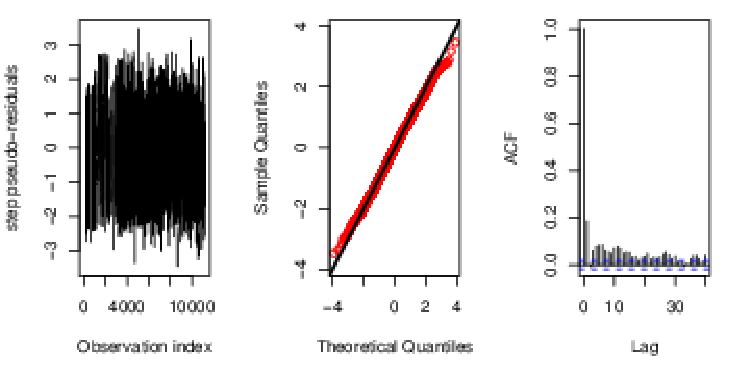
\includegraphics[width=\textwidth]{plot_garterSnakePR.pdf}
  \caption{Pseudo-residual plot for the HHMM garter snake example.}
  \label{fig:snakePR}
\end{figure}
\noindent and simulate from our fitted HHMM using \verb|simHierData|:
\begin{knitrout}
\definecolor{shadecolor}{rgb}{0.969, 0.969, 0.969}\color{fgcolor}\begin{kframe}
\begin{alltt}
\hlstd{obsPerLevel} \hlkwb{<-} \hlstd{data.tree}\hlopt{::}\hlstd{Node}\hlopt{$}\hlkwd{new}\hlstd{(}\hlstr{"simHierData"}\hlstd{)}

\hlcom{# number of level 1 observations}
\hlstd{obsPerLevel}\hlopt{$}\hlkwd{AddChild}\hlstd{(}\hlstr{"level1"}\hlstd{,}\hlkwc{obs}\hlstd{=M)}

\hlcom{# number of level 2 observations that follow each level 1 observation}
\hlstd{obsPerLevel}\hlopt{$}\hlkwd{AddChild}\hlstd{(}\hlstr{"level2"}\hlstd{,}\hlkwc{obs}\hlstd{=}\hlkwd{dim}\hlstd{(dataAr)[}\hlnum{1}\hlstd{])}

\hlstd{simHHMM} \hlkwb{<-} \hlkwd{simHierData}\hlstd{(}\hlkwc{nbAnimals}\hlstd{=W,}
                       \hlkwc{model}\hlstd{=hhmm,}
                       \hlkwc{obsPerLevel} \hlstd{= obsPerLevel,} \hlkwc{states} \hlstd{=} \hlnum{TRUE}\hlstd{)}
\end{alltt}


{\ttfamily\noindent\itshape\color{messagecolor}{\#\# =======================================================================}}

{\ttfamily\noindent\itshape\color{messagecolor}{\#\# Simulating hierarchical HMM with 9 states and 1 data stream}}

{\ttfamily\noindent\itshape\color{messagecolor}{\#\# -----------------------------------------------------------------------}}

{\ttfamily\noindent\itshape\color{messagecolor}{\#\#\ \ step \textasciitilde{} gamma(mean: custom, sd: custom)}}

{\ttfamily\noindent\itshape\color{messagecolor}{\#\# \\\#\#\ \ Transition probability matrix formula: \textasciitilde{}0 + I((level == "{}1"{}) * 1) + I((level == "{}2i"{}) * 1) + I((level == "{}2"{}) * 1)}}

{\ttfamily\noindent\itshape\color{messagecolor}{\#\# \\\#\#\ \ Initial distribution formula: \textasciitilde{}1}}

{\ttfamily\noindent\itshape\color{messagecolor}{\#\# =======================================================================}}

{\ttfamily\noindent\itshape\color{messagecolor}{\#\# DONE}}\begin{alltt}
\hlkwd{head}\hlstd{(simHHMM)}
\end{alltt}
\begin{verbatim}
##   ID level     step        x  y states
## 1  1     1       NA       NA NA      4
## 2  1    2i       NA       NA NA      6
## 3  1     2 1.992639 0.000000  0      6
## 4  1     2 1.182153 1.992639  0      5
## 5  1     2 1.045767 3.174792  0      5
## 6  1     2 1.285761 4.220559  0      6
\end{verbatim}
\end{kframe}
\end{knitrout}

\subsubsection{Atlantic cod}
\label{sec:atlanticCod}
Now we will demonstrate how HHMMs with data streams observed at multiple time scales can be fitted using \verb|momentuHMM|. In their Atlantic cod example, \cite{AdamEtAl2019} fit a 9-state HHMM to coarse-scale horizontal (i.e., step length and turn angle) and fine-scale vertical movement data. The coarse-scale states were ``resting/foraging'' (hereafter ``resForage''), ``mobile/foraging'' (hereafter ``mobForage''), and ``travelling/migrating'' (hereafter ``transit''), each of which was composed of three fine-scale states. To begin our analysis, we must first load and prepare the data \citep[available for download from][]{AdamEtAl2019}:

\begin{knitrout}
\definecolor{shadecolor}{rgb}{0.969, 0.969, 0.969}\color{fgcolor}\begin{kframe}
\begin{alltt}
\hlcom{# load the data from Adam et al }
\hlkwd{load}\hlstd{(}\hlstr{"Atlantic_cod_data_set.RData"}\hlstd{)}
\end{alltt}
\end{kframe}
\end{knitrout}
\begin{knitrout}
\definecolor{shadecolor}{rgb}{0.969, 0.969, 0.969}\color{fgcolor}\begin{kframe}
\begin{alltt}
\hlcom{# coarse-scale data}
\hlstd{data} \hlkwb{<-} \hlkwd{data.frame}\hlstd{(}\hlkwc{level}\hlstd{=}\hlstr{"1"}\hlstd{,}
                   \hlkwc{step}\hlstd{=steps,}
                   \hlkwc{angle}\hlstd{=angles,}
                   \hlkwc{vertical}\hlstd{=}\hlnum{NA}\hlstd{,}
                   \hlkwc{time}\hlstd{=}\hlnum{0}\hlstd{)}

\hlcom{### add extra rows for fine-scale data}
\hlcom{# level=1  indicates when coarse-scale behavior switching can occur }
\hlcom{# level=2i indicates start of each fine-scale interval}
\hlcom{# level=2  indicates when fine-scale behavior switching can occur}
\hlstd{codData} \hlkwb{<-} \hlkwa{NULL}
\hlstd{timeSeq} \hlkwb{<-} \hlkwd{seq}\hlstd{(}\hlkwc{from}\hlstd{=}\hlnum{0}\hlstd{,}\hlkwc{to}\hlstd{=}\hlnum{23}\hlopt{+}\hlnum{5}\hlopt{/}\hlnum{6}\hlstd{,}\hlkwc{length}\hlstd{=}\hlnum{144}\hlstd{)} \hlcom{# time of day covariate}
\hlkwa{for}\hlstd{(i} \hlkwa{in} \hlnum{1}\hlopt{:}\hlkwd{nrow}\hlstd{(data))\{}
  \hlstd{fineInd} \hlkwb{<-} \hlkwd{data.frame}\hlstd{(}\hlkwc{level}\hlstd{=}\hlstr{"2"}\hlstd{,}
                        \hlkwc{step}\hlstd{=}\hlnum{NA}\hlstd{,}
                        \hlkwc{angle}\hlstd{=}\hlnum{NA}\hlstd{,}
                        \hlkwc{vertical}\hlstd{=verticals[[i]],}
                        \hlkwc{time}\hlstd{=timeSeq)}
  \hlstd{tmp} \hlkwb{<-} \hlkwd{rbind}\hlstd{(data[i,,}\hlkwc{drop}\hlstd{=}\hlnum{FALSE}\hlstd{],}
               \hlkwd{data.frame}\hlstd{(}\hlkwc{level}\hlstd{=}\hlstr{"2i"}\hlstd{,}
                          \hlkwc{step}\hlstd{=}\hlnum{NA}\hlstd{,}
                          \hlkwc{angle}\hlstd{=}\hlnum{NA}\hlstd{,}
                          \hlkwc{vertical}\hlstd{=}\hlnum{NA}\hlstd{,}
                          \hlkwc{time}\hlstd{=}\hlnum{0}\hlstd{),}
               \hlstd{fineInd)}
  \hlstd{codData} \hlkwb{<-} \hlkwd{rbind}\hlstd{(codData,tmp)}
\hlstd{\}}

\hlcom{# prepare hierarchical data}
\hlstd{codData} \hlkwb{<-} \hlkwd{prepData}\hlstd{(codData,} \hlkwc{coordNames}\hlstd{=}\hlkwa{NULL}\hlstd{,}
                    \hlkwc{covNames}\hlstd{=}\hlstr{"time"}\hlstd{,}
                    \hlkwc{hierLevels}\hlstd{=}\hlkwd{c}\hlstd{(}\hlstr{"1"}\hlstd{,}\hlstr{"2i"}\hlstd{,}\hlstr{"2"}\hlstd{))}
\hlkwd{head}\hlstd{(codData)}
\end{alltt}
\begin{verbatim}
##        ID level     step angle vertical      time
## 1 Animal1     1 5.236266    NA       NA 0.0000000
## 2 Animal1    2i       NA    NA       NA 0.0000000
## 3 Animal1     2       NA    NA   0.1285 0.0000000
## 4 Animal1     2       NA    NA   0.0499 0.1666667
## 5 Animal1     2       NA    NA   0.1417 0.3333333
## 6 Animal1     2       NA    NA   0.1713 0.5000000
\end{verbatim}
\begin{alltt}
\hlcom{# data summary}
\hlkwd{summary}\hlstd{(codData,}\hlkwc{dataNames}\hlstd{=}\hlkwd{names}\hlstd{(codData)[}\hlopt{-}\hlnum{1}\hlstd{])}
\end{alltt}
\begin{verbatim}
## Hierarchical HMM data for 1 individual:
## 
## Animal1 -- 42486 observations
## 
## 
## Data summaries:
## 
##  level           step           angle          vertical     
##  1 :  291   Min.   : 0.21   Min.   :-3.12   Min.   : 0.000  
##  2i:  291   1st Qu.: 2.86   1st Qu.:-0.36   1st Qu.: 0.083  
##  2 :41904   Median : 5.49   Median : 0.01   Median : 0.182  
##             Mean   : 8.24   Mean   :-0.03   Mean   : 0.418  
##             3rd Qu.:11.89   3rd Qu.: 0.34   3rd Qu.: 0.440  
##             Max.   :31.49   Max.   : 3.12   Max.   :18.223  
##             NA's   :42196   NA's   :42197   NA's   :582     
##       time     
##  Min.   : 0.0  
##  1st Qu.: 5.7  
##  Median :11.8  
##  Mean   :11.8  
##  3rd Qu.:17.8  
##  Max.   :23.8  
## 
\end{verbatim}
\end{kframe}
\end{knitrout}

From sections \ref{sec:harborPorpoise} and \ref{sec:garterSnake}, we should now be familiar with how to specify HHMMs with state transitions at multiple time scales. We will therefore focus on how to accommodate data streams that are observed at multiple time scales here, but complete details and code for fitting this model can be found in the ``codExample.R'' script in the \verb|momentuHMM| ``vignettes'' source directory (or at \url{https://github.com/bmcclintock/momentuHMM}). First we specify the hierarchical nature of the states as a \verb|data.tree| Node:
\begin{knitrout}
\definecolor{shadecolor}{rgb}{0.969, 0.969, 0.969}\color{fgcolor}\begin{kframe}
\begin{alltt}
\hlcom{### define hierarchical HMM}
\hlcom{# states 1-3 = coarse state 1 (resident/foraging)}
\hlcom{# states 4-6 = coarse state 2 (mobile/foraging)}
\hlcom{# states 7-9 = coarse state 3 (travelling/migrating)}
\hlstd{hierStates} \hlkwb{<-} \hlstd{data.tree}\hlopt{::}\hlstd{Node}\hlopt{$}\hlkwd{new}\hlstd{(}\hlstr{"cod HHMM states"}\hlstd{)}
\hlstd{hierStates}\hlopt{$}\hlkwd{AddChild}\hlstd{(}\hlstr{"resForage"}\hlstd{)}   \hlcom{# resident/foraging}
\hlstd{hierStates}\hlopt{$}\hlstd{resForage}\hlopt{$}\hlkwd{AddChild}\hlstd{(}\hlstr{"rF1"}\hlstd{,} \hlkwc{state}\hlstd{=}\hlnum{1}\hlstd{)}
\hlstd{hierStates}\hlopt{$}\hlstd{resForage}\hlopt{$}\hlkwd{AddChild}\hlstd{(}\hlstr{"rF2"}\hlstd{,} \hlkwc{state}\hlstd{=}\hlnum{2}\hlstd{)}
\hlstd{hierStates}\hlopt{$}\hlstd{resForage}\hlopt{$}\hlkwd{AddChild}\hlstd{(}\hlstr{"rF3"}\hlstd{,} \hlkwc{state}\hlstd{=}\hlnum{3}\hlstd{)}
\hlstd{hierStates}\hlopt{$}\hlkwd{AddChild}\hlstd{(}\hlstr{"mobForage"}\hlstd{)}  \hlcom{# mobile/foraging}
\hlstd{hierStates}\hlopt{$}\hlstd{mobForage}\hlopt{$}\hlkwd{AddChild}\hlstd{(}\hlstr{"mF1"}\hlstd{,} \hlkwc{state}\hlstd{=}\hlnum{4}\hlstd{)}
\hlstd{hierStates}\hlopt{$}\hlstd{mobForage}\hlopt{$}\hlkwd{AddChild}\hlstd{(}\hlstr{"mF2"}\hlstd{,} \hlkwc{state}\hlstd{=}\hlnum{5}\hlstd{)}
\hlstd{hierStates}\hlopt{$}\hlstd{mobForage}\hlopt{$}\hlkwd{AddChild}\hlstd{(}\hlstr{"mF3"}\hlstd{,} \hlkwc{state}\hlstd{=}\hlnum{6}\hlstd{)}
\hlstd{hierStates}\hlopt{$}\hlkwd{AddChild}\hlstd{(}\hlstr{"transit"}\hlstd{)}    \hlcom{# travelling/migrating}
\hlstd{hierStates}\hlopt{$}\hlstd{transit}\hlopt{$}\hlkwd{AddChild}\hlstd{(}\hlstr{"t1"}\hlstd{,} \hlkwc{state}\hlstd{=}\hlnum{7}\hlstd{)}
\hlstd{hierStates}\hlopt{$}\hlstd{transit}\hlopt{$}\hlkwd{AddChild}\hlstd{(}\hlstr{"t2"}\hlstd{,} \hlkwc{state}\hlstd{=}\hlnum{8}\hlstd{)}
\hlstd{hierStates}\hlopt{$}\hlstd{transit}\hlopt{$}\hlkwd{AddChild}\hlstd{(}\hlstr{"t3"}\hlstd{,} \hlkwc{state}\hlstd{=}\hlnum{9}\hlstd{)}

\hlkwd{plot}\hlstd{(hierStates)}
\end{alltt}
\end{kframe}
\includegraphics[width=\maxwidth]{figure/cod-2-1} 

\end{knitrout}

Next we specify the hierarchical nature of the data streams as a \verb|data.tree| Node:
\begin{knitrout}
\definecolor{shadecolor}{rgb}{0.969, 0.969, 0.969}\color{fgcolor}\begin{kframe}
\begin{alltt}
\hlcom{# data stream distributions}
\hlcom{# level 1 = coarse level (step="gamma", angle="vm")}
\hlcom{# level 2 = fine level (vertical="gamma")}
\hlstd{hierDist} \hlkwb{<-} \hlstd{data.tree}\hlopt{::}\hlstd{Node}\hlopt{$}\hlkwd{new}\hlstd{(}\hlstr{"cod HHMM dist"}\hlstd{)}
\hlstd{hierDist}\hlopt{$}\hlkwd{AddChild}\hlstd{(}\hlstr{"level1"}\hlstd{)}
\hlstd{hierDist}\hlopt{$}\hlstd{level1}\hlopt{$}\hlkwd{AddChild}\hlstd{(}\hlstr{"step"}\hlstd{,} \hlkwc{dist}\hlstd{=}\hlstr{"gamma"}\hlstd{)}
\hlstd{hierDist}\hlopt{$}\hlstd{level1}\hlopt{$}\hlkwd{AddChild}\hlstd{(}\hlstr{"angle"}\hlstd{,} \hlkwc{dist}\hlstd{=}\hlstr{"vm"}\hlstd{)}
\hlstd{hierDist}\hlopt{$}\hlkwd{AddChild}\hlstd{(}\hlstr{"level2"}\hlstd{)}
\hlstd{hierDist}\hlopt{$}\hlstd{level2}\hlopt{$}\hlkwd{AddChild}\hlstd{(}\hlstr{"vertical"}\hlstd{,} \hlkwc{dist}\hlstd{=}\hlstr{"gamma"}\hlstd{)}

\hlkwd{plot}\hlstd{(hierDist)}
\end{alltt}
\end{kframe}
\includegraphics[width=\maxwidth]{figure/cod-3-1} 

\end{knitrout}

We then constrain the fine-scale states within each coarse-scale state to have the same parameters for the ``step'' and ``angle'' distributions using the \verb|DM| argument:
\begin{knitrout}
\definecolor{shadecolor}{rgb}{0.969, 0.969, 0.969}\color{fgcolor}\begin{kframe}
\begin{alltt}
\hlstd{nbStates} \hlkwb{<-} \hlkwd{length}\hlstd{(hierStates}\hlopt{$}\hlkwd{Get}\hlstd{(}\hlstr{"state"}\hlstd{,}\hlkwc{filterFun}\hlstd{=data.tree}\hlopt{::}\hlstd{isLeaf))}

\hlcom{# constrain coarse-scale parameters for fine-scale states}
\hlstd{DM} \hlkwb{<-} \hlkwd{list}\hlstd{(}\hlkwc{step}\hlstd{=}\hlkwd{matrix}\hlstd{(}\hlkwd{kronecker}\hlstd{(}\hlkwd{diag}\hlstd{(}\hlnum{6}\hlstd{),}\hlkwd{c}\hlstd{(}\hlnum{1}\hlstd{,}\hlnum{1}\hlstd{,}\hlnum{1}\hlstd{)),}
                       \hlkwc{nrow}\hlstd{=}\hlnum{2}\hlopt{*}\hlstd{nbStates,}
                       \hlkwc{ncol}\hlstd{=}\hlnum{6}\hlstd{,}
                       \hlkwc{dimnames}\hlstd{=}\hlkwd{list}\hlstd{(}\hlkwd{paste0}\hlstd{(}\hlkwd{rep}\hlstd{(}\hlkwd{c}\hlstd{(}\hlstr{"mean_"}\hlstd{,}\hlstr{"sd_"}\hlstd{),}\hlkwc{each}\hlstd{=nbStates)}
                                            \hlstd{,}\hlnum{1}\hlopt{:}\hlstd{nbStates),}
                                     \hlkwd{c}\hlstd{(}\hlkwd{paste0}\hlstd{(}\hlkwd{rep}\hlstd{(}\hlkwd{c}\hlstd{(}\hlstr{"mean_"}\hlstd{,}\hlstr{"sd_"}\hlstd{),}\hlkwc{each}\hlstd{=}\hlnum{3}\hlstd{),}
                                              \hlnum{1}\hlopt{:}\hlkwd{length}\hlstd{(hierStates}\hlopt{$}\hlstd{children),}
                                              \hlstr{":(Intercept)"}\hlstd{)))))}
\hlstd{DM}\hlopt{$}\hlstd{angle} \hlkwb{<-} \hlstd{DM}\hlopt{$}\hlstd{step}
\hlkwd{dimnames}\hlstd{(DM}\hlopt{$}\hlstd{angle)} \hlkwb{<-} \hlkwd{list}\hlstd{(}\hlkwd{paste0}\hlstd{(}\hlkwd{rep}\hlstd{(}\hlkwd{c}\hlstd{(}\hlstr{"mean_"}\hlstd{,}\hlstr{"concentration_"}\hlstd{),}\hlkwc{each}\hlstd{=nbStates)}
                                  \hlstd{,}\hlnum{1}\hlopt{:}\hlstd{nbStates),}
                           \hlkwd{c}\hlstd{(}\hlkwd{paste0}\hlstd{(}\hlkwd{rep}\hlstd{(}\hlkwd{c}\hlstd{(}\hlstr{"mean_"}\hlstd{,}\hlstr{"concentration_"}\hlstd{),}\hlkwc{each}\hlstd{=}\hlnum{3}\hlstd{),}
                                    \hlnum{1}\hlopt{:}\hlkwd{length}\hlstd{(hierStates}\hlopt{$}\hlstd{children),}
                                    \hlstr{":(Intercept)"}\hlstd{)))}
\end{alltt}
\end{kframe}
\end{knitrout}
\noindent and obtain starting values on the working scale using \verb|getParDM|:
\begin{knitrout}
\definecolor{shadecolor}{rgb}{0.969, 0.969, 0.969}\color{fgcolor}\begin{kframe}
\begin{alltt}
\hlcom{### defining start values based on those reported by Adam et al}
\hlstd{hm.mu0} \hlkwb{<-} \hlkwd{c}\hlstd{(}\hlnum{5.482}\hlstd{,} \hlnum{6.786}\hlstd{,} \hlnum{14.914}\hlstd{)}
\hlstd{hm.sigma0} \hlkwb{<-} \hlkwd{c}\hlstd{(}\hlnum{4.27}\hlstd{,} \hlnum{4.714}\hlstd{,} \hlnum{11.242}\hlstd{)}

\hlstd{ha.mu0} \hlkwb{<-} \hlkwd{c}\hlstd{(}\hlnum{0.011}\hlstd{,} \hlopt{-}\hlnum{0.299}\hlstd{,} \hlnum{0.044}\hlstd{)}
\hlstd{ha.kappa0} \hlkwb{<-} \hlkwd{c}\hlstd{(}\hlnum{1.571}\hlstd{,} \hlnum{1.426}\hlstd{,} \hlnum{2.15}\hlstd{)}

\hlstd{vm.mu0} \hlkwb{<-} \hlstd{vm.sigma0} \hlkwb{<-} \hlstd{vm.pi0} \hlkwb{<-} \hlkwd{list}\hlstd{()}
\hlstd{vm.mu0[[}\hlnum{1}\hlstd{]]} \hlkwb{<-} \hlkwd{c}\hlstd{(}\hlnum{0.116}\hlstd{,} \hlnum{0.303}\hlstd{,} \hlnum{0.691}\hlstd{)}
\hlstd{vm.mu0[[}\hlnum{2}\hlstd{]]} \hlkwb{<-} \hlkwd{c}\hlstd{(}\hlnum{0.109}\hlstd{,} \hlnum{0.056}\hlstd{,} \hlnum{0.351}\hlstd{)}
\hlstd{vm.mu0[[}\hlnum{3}\hlstd{]]} \hlkwb{<-} \hlkwd{c}\hlstd{(}\hlnum{0.125}\hlstd{,} \hlnum{0.514}\hlstd{,} \hlnum{1.987}\hlstd{)}

\hlstd{vm.sigma0[[}\hlnum{1}\hlstd{]]} \hlkwb{<-} \hlkwd{c}\hlstd{(}\hlnum{0.096}\hlstd{,} \hlnum{0.261}\hlstd{,} \hlnum{0.636}\hlstd{)}
\hlstd{vm.sigma0[[}\hlnum{2}\hlstd{]]} \hlkwb{<-} \hlkwd{c}\hlstd{(}\hlnum{0.043}\hlstd{,} \hlnum{0.047}\hlstd{,} \hlnum{0.342}\hlstd{)}
\hlstd{vm.sigma0[[}\hlnum{3}\hlstd{]]} \hlkwb{<-} \hlkwd{c}\hlstd{(}\hlnum{0.109}\hlstd{,} \hlnum{0.462}\hlstd{,} \hlnum{1.878}\hlstd{)}

\hlstd{vm.pi0[[}\hlnum{1}\hlstd{]]} \hlkwb{<-} \hlkwd{c}\hlstd{(}\hlnum{0.014}\hlstd{,} \hlnum{0.003}\hlstd{,} \hlnum{1.050e-06}\hlstd{)}
\hlstd{vm.pi0[[}\hlnum{2}\hlstd{]]} \hlkwb{<-} \hlkwd{c}\hlstd{(}\hlnum{1.791e-08}\hlstd{,} \hlnum{0.035}\hlstd{,} \hlnum{0.002}\hlstd{)}
\hlstd{vm.pi0[[}\hlnum{3}\hlstd{]]} \hlkwb{<-} \hlkwd{c}\hlstd{(}\hlnum{0.012}\hlstd{,} \hlnum{2.933e-04}\hlstd{,} \hlnum{3.462e-09}\hlstd{)}

\hlstd{Par0} \hlkwb{<-} \hlkwd{list}\hlstd{(}\hlkwc{step}\hlstd{=}\hlkwd{c}\hlstd{(}\hlkwd{rep}\hlstd{(hm.mu0,}\hlkwc{each}\hlstd{=}\hlnum{3}\hlstd{),}\hlkwd{rep}\hlstd{(hm.sigma0,}\hlkwc{each}\hlstd{=}\hlnum{3}\hlstd{)),}
             \hlkwc{angle}\hlstd{=}\hlkwd{c}\hlstd{(}\hlkwd{rep}\hlstd{(ha.mu0,}\hlkwc{each}\hlstd{=}\hlnum{3}\hlstd{),}\hlkwd{rep}\hlstd{(ha.kappa0,}\hlkwc{each}\hlstd{=}\hlnum{3}\hlstd{)),}
             \hlkwc{vertical}\hlstd{=}\hlkwd{c}\hlstd{(}\hlkwd{unlist}\hlstd{(vm.mu0),}\hlkwd{unlist}\hlstd{(vm.sigma0),}\hlkwd{unlist}\hlstd{(vm.pi0)))}

\hlcom{# starting values for data stream parameters on the working scale}
\hlstd{Par} \hlkwb{<-} \hlkwd{getParDM}\hlstd{(codData,}
                \hlkwc{hierStates}\hlstd{=hierStates,}
                \hlkwc{hierDist}\hlstd{=hierDist,}
                \hlkwc{Par}\hlstd{=Par0,}
                \hlkwc{DM}\hlstd{=DM,}
                \hlkwc{estAngleMean} \hlstd{=} \hlkwd{list}\hlstd{(}\hlkwc{angle}\hlstd{=}\hlnum{TRUE}\hlstd{))}
\end{alltt}
\end{kframe}
\end{knitrout}

\cite{AdamEtAl2019} included a periodic time-of-day covariate on the fine-scale state transition probabilities, and we specify this via the \verb|hierFormula| argument:
\begin{knitrout}
\definecolor{shadecolor}{rgb}{0.969, 0.969, 0.969}\color{fgcolor}\begin{kframe}
\begin{alltt}
\hlcom{# define hierarchical t.p.m. formula(s)}
\hlstd{hierFormula} \hlkwb{<-} \hlstd{data.tree}\hlopt{::}\hlstd{Node}\hlopt{$}\hlkwd{new}\hlstd{(}\hlstr{"cod HHMM formula"}\hlstd{)}
\hlstd{hierFormula}\hlopt{$}\hlkwd{AddChild}\hlstd{(}\hlstr{"level1"}\hlstd{,} \hlkwc{formula}\hlstd{=}\hlopt{~}\hlnum{1}\hlstd{)}
\hlstd{hierFormula}\hlopt{$}\hlkwd{AddChild}\hlstd{(}\hlstr{"level2"}\hlstd{,} \hlkwc{formula}\hlstd{=}\hlopt{~}\hlkwd{cosinor}\hlstd{(time,} \hlkwc{period}\hlstd{=}\hlnum{24}\hlstd{))}
\end{alltt}
\end{kframe}
\end{knitrout}

All that remains is (optionally) specifying starting values for the initial distribution (\verb|hierDelta|) and t.p.m. (\verb|hierBeta|) parameters, which we'll base on those reported by \cite{AdamEtAl2019} to speed up the optimization:
\begin{knitrout}
\definecolor{shadecolor}{rgb}{0.969, 0.969, 0.969}\color{fgcolor}\begin{kframe}
\begin{alltt}
\hlstd{hierBeta} \hlkwb{<-} \hlstd{data.tree}\hlopt{::}\hlstd{Node}\hlopt{$}\hlkwd{new}\hlstd{(}\hlstr{"cod beta"}\hlstd{)}
\hlstd{hierBeta}\hlopt{$}\hlkwd{AddChild}\hlstd{(}\hlstr{"level1"}\hlstd{,}
          \hlkwc{beta}\hlstd{=}\hlkwd{matrix}\hlstd{(}\hlkwd{c}\hlstd{(}\hlopt{-}\hlnum{18.585}\hlstd{,} \hlopt{-}\hlnum{2.86}\hlstd{,} \hlopt{-}\hlnum{2.551}\hlstd{,} \hlopt{-}\hlnum{1.641}\hlstd{,} \hlopt{-}\hlnum{2.169}\hlstd{,} \hlopt{-}\hlnum{2.415}\hlstd{),}
                      \hlkwc{nrow}\hlstd{=}\hlnum{1}\hlstd{,}
                      \hlkwc{ncol}\hlstd{=}\hlkwd{length}\hlstd{(hierStates}\hlopt{$}\hlstd{children)}
                       \hlopt{*}\hlstd{(}\hlkwd{length}\hlstd{(hierStates}\hlopt{$}\hlstd{children)}\hlopt{-}\hlnum{1}\hlstd{)))}
\hlstd{hierBeta}\hlopt{$}\hlkwd{AddChild}\hlstd{(}\hlstr{"level2"}\hlstd{)}
\hlstd{hierBeta}\hlopt{$}\hlstd{level2}\hlopt{$}\hlkwd{AddChild}\hlstd{(}\hlstr{"resForage"}\hlstd{,}
          \hlkwc{beta}\hlstd{=}\hlkwd{matrix}\hlstd{(}\hlkwd{c}\hlstd{(}\hlopt{-}\hlnum{2.562}\hlstd{,} \hlopt{-}\hlnum{3.403}\hlstd{,}  \hlnum{2.765}\hlstd{,} \hlopt{-}\hlnum{1.607}\hlstd{,}  \hlnum{2.273}\hlstd{,}  \hlnum{4.842}\hlstd{,}
                        \hlopt{-}\hlnum{0.665}\hlstd{,}  \hlopt{-}\hlnum{0.26}\hlstd{,} \hlopt{-}\hlnum{0.681}\hlstd{,} \hlopt{-}\hlnum{0.149}\hlstd{,} \hlopt{-}\hlnum{2.728}\hlstd{,} \hlopt{-}\hlnum{2.798}\hlstd{,}
                        \hlopt{-}\hlnum{0.027}\hlstd{,}   \hlnum{0.26}\hlstd{,}  \hlnum{0.191}\hlstd{,}  \hlnum{0.667}\hlstd{,}  \hlnum{0.123}\hlstd{,} \hlopt{-}\hlnum{0.262}\hlstd{),}
                      \hlkwc{nrow}\hlstd{=}\hlnum{3}\hlstd{,}
                      \hlkwc{ncol}\hlstd{=}\hlkwd{length}\hlstd{(hierStates}\hlopt{$}\hlstd{resForage}\hlopt{$}\hlstd{children)}
                       \hlopt{*}\hlstd{(}\hlkwd{length}\hlstd{(hierStates}\hlopt{$}\hlstd{resForage}\hlopt{$}\hlstd{children)}\hlopt{-}\hlnum{1}\hlstd{),}
                      \hlkwc{byrow}\hlstd{=}\hlnum{TRUE}\hlstd{))}
\hlstd{hierBeta}\hlopt{$}\hlstd{level2}\hlopt{$}\hlkwd{AddChild}\hlstd{(}\hlstr{"mobForage"}\hlstd{,}
          \hlkwc{beta}\hlstd{=}\hlkwd{matrix}\hlstd{(}\hlkwd{c}\hlstd{(}\hlopt{-}\hlnum{2.156}\hlstd{,} \hlopt{-}\hlnum{3.662}\hlstd{,}   \hlnum{3.01}\hlstd{,}  \hlnum{0.597}\hlstd{,} \hlopt{-}\hlnum{0.313}\hlstd{,}  \hlnum{2.897}\hlstd{,}
                         \hlnum{0.067}\hlstd{,}  \hlopt{-}\hlnum{1.22}\hlstd{,} \hlopt{-}\hlnum{0.799}\hlstd{,} \hlopt{-}\hlnum{0.797}\hlstd{,}   \hlnum{0.15}\hlstd{,}  \hlnum{0.379}\hlstd{,}
                        \hlopt{-}\hlnum{0.112}\hlstd{,} \hlopt{-}\hlnum{0.195}\hlstd{,} \hlopt{-}\hlnum{0.269}\hlstd{,} \hlopt{-}\hlnum{0.215}\hlstd{,}  \hlnum{1.539}\hlstd{,}  \hlnum{0.728}\hlstd{),}
                      \hlkwc{nrow}\hlstd{=}\hlnum{3}\hlstd{,}
                      \hlkwc{ncol}\hlstd{=}\hlkwd{length}\hlstd{(hierStates}\hlopt{$}\hlstd{mobForage}\hlopt{$}\hlstd{children)}
                       \hlopt{*}\hlstd{(}\hlkwd{length}\hlstd{(hierStates}\hlopt{$}\hlstd{mobForage}\hlopt{$}\hlstd{children)}\hlopt{-}\hlnum{1}\hlstd{),}
                      \hlkwc{byrow}\hlstd{=}\hlnum{TRUE}\hlstd{))}
\hlstd{hierBeta}\hlopt{$}\hlstd{level2}\hlopt{$}\hlkwd{AddChild}\hlstd{(}\hlstr{"transit"}\hlstd{,}
          \hlkwc{beta}\hlstd{=}\hlkwd{matrix}\hlstd{(}\hlkwd{c}\hlstd{(}\hlopt{-}\hlnum{2.53}\hlstd{,} \hlopt{-}\hlnum{4.279}\hlstd{,}  \hlnum{2.507}\hlstd{,} \hlopt{-}\hlnum{0.228}\hlstd{,} \hlnum{10.803}\hlstd{,} \hlnum{12.873}\hlstd{,}
                        \hlopt{-}\hlnum{0.04}\hlstd{,}  \hlnum{1.221}\hlstd{,} \hlopt{-}\hlnum{0.301}\hlstd{,}  \hlnum{0.284}\hlstd{,} \hlopt{-}\hlnum{0.106}\hlstd{,} \hlopt{-}\hlnum{0.077}\hlstd{,}
                        \hlnum{0.629}\hlstd{,} \hlopt{-}\hlnum{0.226}\hlstd{,} \hlopt{-}\hlnum{0.253}\hlstd{,} \hlopt{-}\hlnum{0.303}\hlstd{,}  \hlnum{0.011}\hlstd{,}  \hlnum{0.036}\hlstd{),}
                      \hlkwc{nrow}\hlstd{=}\hlnum{3}\hlstd{,}
                      \hlkwc{ncol}\hlstd{=}\hlkwd{length}\hlstd{(hierStates}\hlopt{$}\hlstd{transit}\hlopt{$}\hlstd{children)}
                       \hlopt{*}\hlstd{(}\hlkwd{length}\hlstd{(hierStates}\hlopt{$}\hlstd{transit}\hlopt{$}\hlstd{children)}\hlopt{-}\hlnum{1}\hlstd{),}
                      \hlkwc{byrow}\hlstd{=}\hlnum{TRUE}\hlstd{))}

\hlstd{hierDelta} \hlkwb{<-} \hlstd{data.tree}\hlopt{::}\hlstd{Node}\hlopt{$}\hlkwd{new}\hlstd{(}\hlstr{"cod delta"}\hlstd{)}
\hlstd{hierDelta}\hlopt{$}\hlkwd{AddChild}\hlstd{(}\hlstr{"level1"}\hlstd{,}\hlkwc{delta}\hlstd{=}\hlkwd{matrix}\hlstd{(}\hlkwd{c}\hlstd{(}\hlnum{15.776}\hlstd{,} \hlnum{4.78}\hlstd{),}\hlnum{1}\hlstd{))}
\hlstd{hierDelta}\hlopt{$}\hlkwd{AddChild}\hlstd{(}\hlstr{"level2"}\hlstd{)}
\hlstd{hierDelta}\hlopt{$}\hlstd{level2}\hlopt{$}\hlkwd{AddChild}\hlstd{(}\hlstr{"resForage"}\hlstd{,}\hlkwc{delta}\hlstd{=}\hlkwd{matrix}\hlstd{(}\hlkwd{c}\hlstd{(}\hlopt{-}\hlnum{0.643}\hlstd{,} \hlopt{-}\hlnum{2.416}\hlstd{),}\hlnum{1}\hlstd{))}
\hlstd{hierDelta}\hlopt{$}\hlstd{level2}\hlopt{$}\hlkwd{AddChild}\hlstd{(}\hlstr{"mobForage"}\hlstd{,}\hlkwc{delta}\hlstd{=}\hlkwd{matrix}\hlstd{(}\hlkwd{c}\hlstd{(}\hlnum{1.181}\hlstd{,} \hlnum{0.46}\hlstd{),}\hlnum{1}\hlstd{))}
\hlstd{hierDelta}\hlopt{$}\hlstd{level2}\hlopt{$}\hlkwd{AddChild}\hlstd{(}\hlstr{"transit"}\hlstd{,}\hlkwc{delta}\hlstd{=}\hlkwd{matrix}\hlstd{(}\hlkwd{c}\hlstd{(}\hlopt{-}\hlnum{0.357}\hlstd{,} \hlopt{-}\hlnum{0.624}\hlstd{),}\hlnum{1}\hlstd{))}

\hlcom{# check hierarchical model specification and parameters}
\hlkwd{checkPar0}\hlstd{(codData,}
          \hlkwc{hierStates} \hlstd{= hierStates,}
          \hlkwc{hierDist} \hlstd{= hierDist,}
          \hlkwc{hierFormula} \hlstd{= hierFormula,}
          \hlkwc{Par0} \hlstd{= Par,} \hlkwc{hierBeta} \hlstd{= hierBeta,} \hlkwc{hierDelta} \hlstd{= hierDelta,}
          \hlkwc{DM} \hlstd{= DM,}
          \hlkwc{estAngleMean} \hlstd{=} \hlkwd{list}\hlstd{(}\hlkwc{angle}\hlstd{=}\hlnum{TRUE}\hlstd{))}
\end{alltt}
\begin{verbatim}
## 
## Regression coeffs for step parameters:
## --------------------------------------
##      mean_1:(Intercept) mean_2:(Intercept) mean_3:(Intercept)
## [1,]            1.70147           1.914862             2.7023
##      sd_1:(Intercept) sd_2:(Intercept) sd_3:(Intercept)
## [1,]         1.451614         1.550537         2.419657
## 
## Regression coeffs for angle parameters:
## ---------------------------------------
##      mean_1:(Intercept) mean_2:(Intercept) mean_3:(Intercept)
## [1,]        0.005500055         -0.1506238         0.02200355
##      concentration_1:(Intercept) concentration_2:(Intercept)
## [1,]                   0.4517124                   0.3548733
##      concentration_3:(Intercept)
## [1,]                   0.7654678
## 
## vertical parameters:
## --------------------
##            rF1   rF2      rF3       mF1   mF2   mF3    t1        t2
## mean     0.116 0.303 6.91e-01 1.090e-01 0.056 0.351 0.125 0.5140000
## sd       0.096 0.261 6.36e-01 4.300e-02 0.047 0.342 0.109 0.4620000
## zeromass 0.014 0.003 1.05e-06 1.791e-08 0.035 0.002 0.012 0.0002933
##                 t3
## mean     1.987e+00
## sd       1.878e+00
## zeromass 3.462e-09
## 
## ----------------------------------------------------------
## Regression coeffs for the transition probabilities (beta):
## ----------------------------------------------------------
## -------------------------  level1  -----------------------
##                        1 -> 4 1 -> 7 4 -> 1 4 -> 7 7 -> 1 7 -> 4
## I((level == "1") * 1) -18.585  -2.86 -2.551 -1.641 -2.169 -2.415
## 
## -------------------------  level2  -----------------------
##                                                   1 -> 2 1 -> 3 2 -> 2
## I((level == "2") * 1)                             -2.562 -3.403  2.765
## I((level == "2") * cosinorCos(time, period = 24)) -0.665 -0.260 -0.681
## I((level == "2") * cosinorSin(time, period = 24)) -0.027  0.260  0.191
##                                                   2 -> 3 3 -> 2 3 -> 3
## I((level == "2") * 1)                             -1.607  2.273  4.842
## I((level == "2") * cosinorCos(time, period = 24)) -0.149 -2.728 -2.798
## I((level == "2") * cosinorSin(time, period = 24))  0.667  0.123 -0.262
## 
##                                                   4 -> 5 4 -> 6 5 -> 5
## I((level == "2") * 1)                             -2.156 -3.662  3.010
## I((level == "2") * cosinorCos(time, period = 24))  0.067 -1.220 -0.799
## I((level == "2") * cosinorSin(time, period = 24)) -0.112 -0.195 -0.269
##                                                   5 -> 6 6 -> 5 6 -> 6
## I((level == "2") * 1)                              0.597 -0.313  2.897
## I((level == "2") * cosinorCos(time, period = 24)) -0.797  0.150  0.379
## I((level == "2") * cosinorSin(time, period = 24)) -0.215  1.539  0.728
## 
##                                                   7 -> 8 7 -> 9 8 -> 8
## I((level == "2") * 1)                             -2.530 -4.279  2.507
## I((level == "2") * cosinorCos(time, period = 24)) -0.040  1.221 -0.301
## I((level == "2") * cosinorSin(time, period = 24))  0.629 -0.226 -0.253
##                                                   8 -> 9 9 -> 8 9 -> 9
## I((level == "2") * 1)                             -0.228 10.803 12.873
## I((level == "2") * cosinorCos(time, period = 24))  0.284 -0.106 -0.077
## I((level == "2") * cosinorSin(time, period = 24)) -0.303  0.011  0.036
## 
## ----------------------------------------------------------
## 
## ----------------------------------------------------------
## Regression coeffs for the initial distribution (delta):
## ----------------------------------------------------------
## ------------------------  level1  ------------------------
##             state 4 state 7
## (Intercept)  15.776    4.78
## 
## ------------------------  level2  ------------------------
##                        state 2 state 3
## I((level == "2i") * 1)  -0.643  -2.416
## 
##                        state 5 state 6
## I((level == "2i") * 1)   1.181    0.46
## 
##                        state 8 state 9
## I((level == "2i") * 1)  -0.357  -0.624
## 
## ----------------------------------------------------------
\end{verbatim}
\end{kframe}
\end{knitrout}
\noindent and we are now ready to fit the HHMM:

\begin{knitrout}
\definecolor{shadecolor}{rgb}{0.969, 0.969, 0.969}\color{fgcolor}\begin{kframe}
\begin{alltt}
\hlstd{hhmm} \hlkwb{<-} \hlkwd{fitHMM}\hlstd{(codData,}
               \hlkwc{hierStates} \hlstd{= hierStates,}
               \hlkwc{hierDist} \hlstd{= hierDist,}
               \hlkwc{hierFormula} \hlstd{= hierFormula,}
               \hlkwc{Par0} \hlstd{= Par,} \hlkwc{hierBeta} \hlstd{= hierBeta,} \hlkwc{hierDelta} \hlstd{= hierDelta,}
               \hlkwc{DM} \hlstd{= DM,}
               \hlkwc{estAngleMean} \hlstd{=} \hlkwd{list}\hlstd{(}\hlkwc{angle}\hlstd{=}\hlnum{TRUE}\hlstd{))}

\hlkwd{plot}\hlstd{(hhmm,} \hlkwc{plotCI}\hlstd{=}\hlnum{TRUE}\hlstd{,} \hlkwc{ask}\hlstd{=}\hlnum{FALSE}\hlstd{)}

\hlcom{# plot stationary distributions and CIs}
\hlkwd{plotStationary}\hlstd{(hhmm,} \hlkwc{plotCI}\hlstd{=}\hlnum{TRUE}\hlstd{)}
\end{alltt}
\end{kframe}
\end{knitrout}
The resulting estimates are virtually identical to \cite{AdamEtAl2019}; the slight differences are attributable to: 1) the forward algorithm in \verb|momentuHMM| (Eq. \ref{eq:HMMlike}) includes a state transition between time steps $t=0$ and $t=1$; and 2) \verb|momentuHMM| uses the lowest fine-scale state index for each coarse-scale state as the mlogit-link reference state for the initial distribution and t.p.m.%; and 3) \cite{AdamEtAl2019} did not include the step length data for the first observation in their likelihood calculation. 
Nevertheless, we can see that the estimated coarse-scale data stream probability distribution (Figure \ref{fig:codDist}) and fine-scale stationary probabilities as a function of time of day (Figure \ref{fig:codStat}) are very similar.
\begin{figure}[htbp]
  \centering
  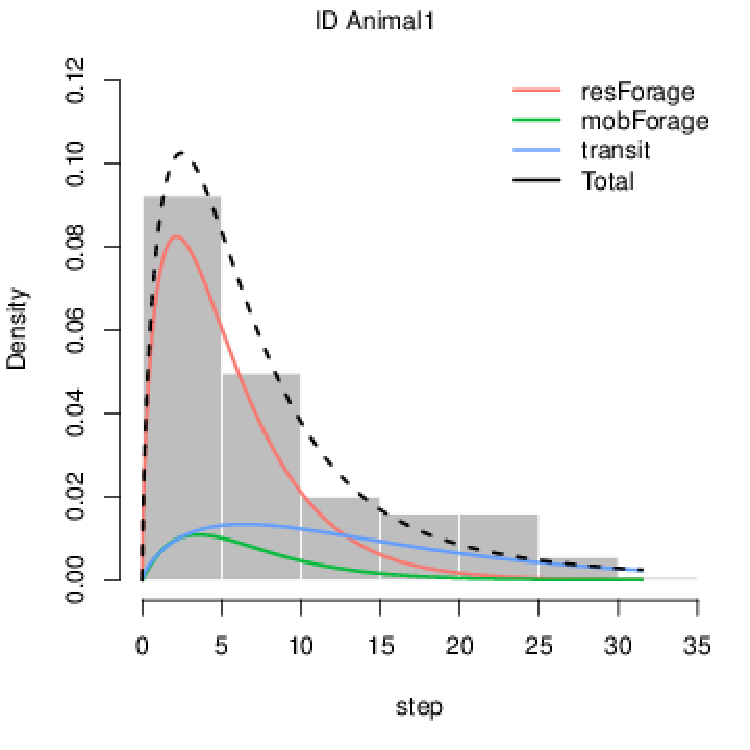
\includegraphics[width=.49\textwidth]{plot_codExample001.pdf}
  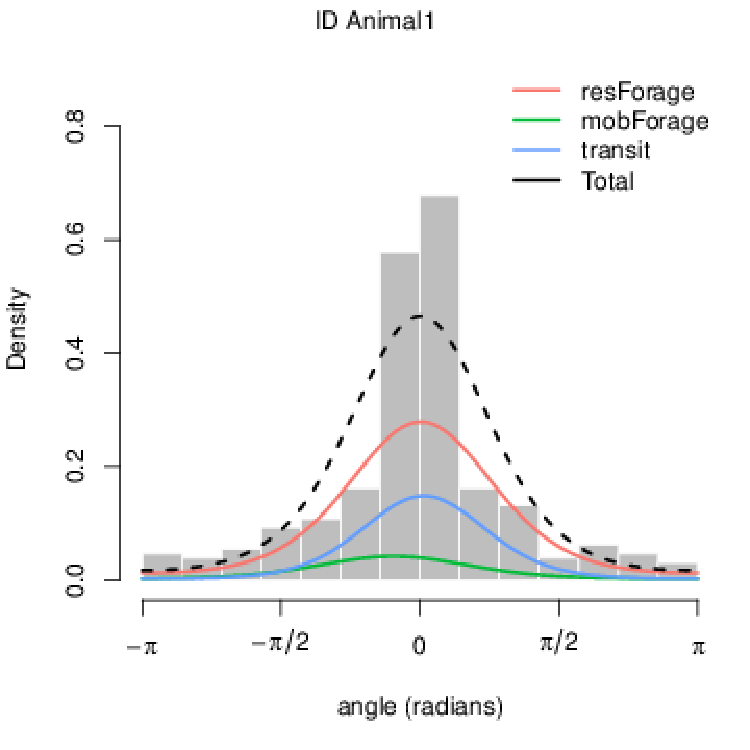
\includegraphics[width=.49\textwidth]{plot_codExample002.pdf}
  \caption{Estimated state-dependent distributions of coarse-scale step lengths (left panel) and turning angles (right panel) of an Atlantic
cod.}
  \label{fig:codDist}
\end{figure}

\begin{figure}[htbp]
  \centering
  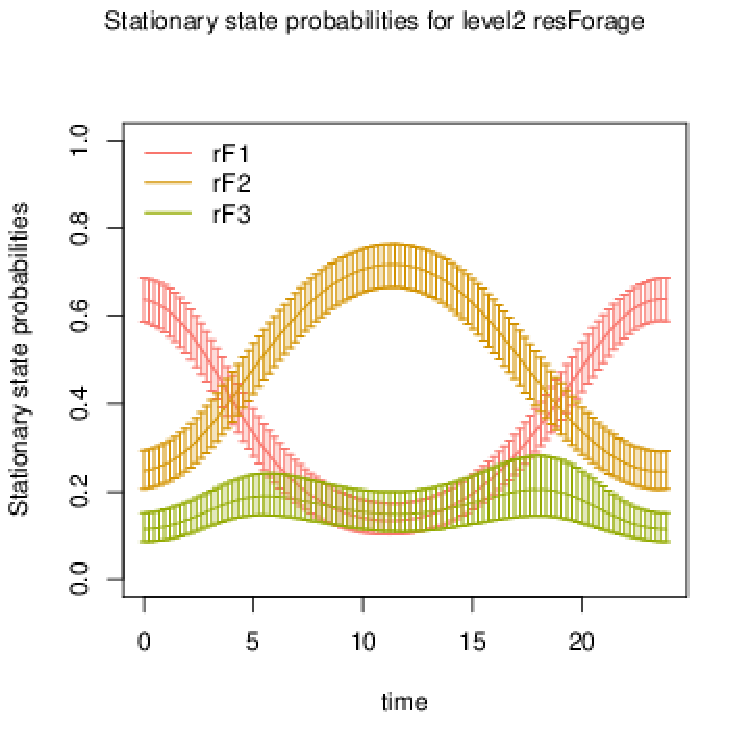
\includegraphics[width=.49\textwidth]{plot_codStationary001.pdf}
  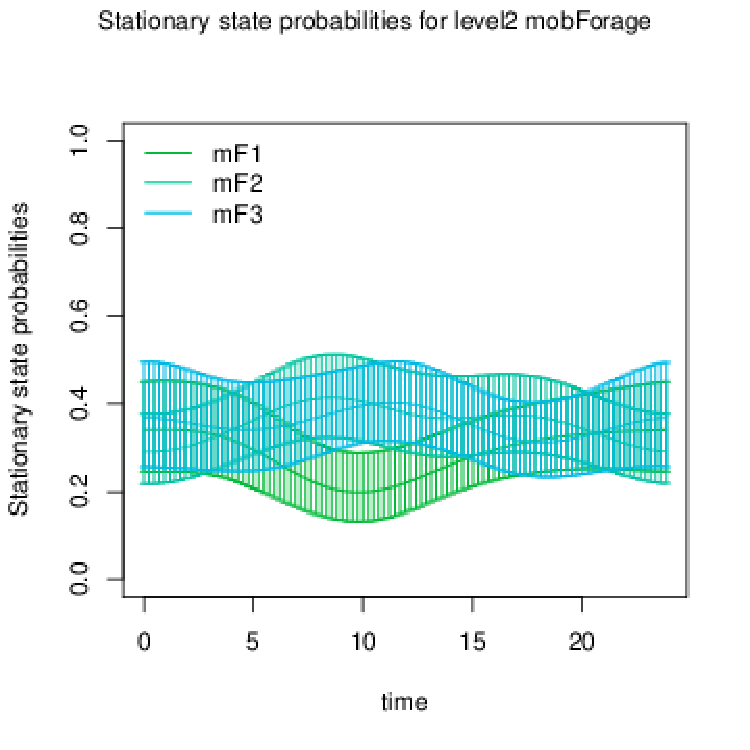
\includegraphics[width=.49\textwidth]{plot_codStationary002.pdf}
  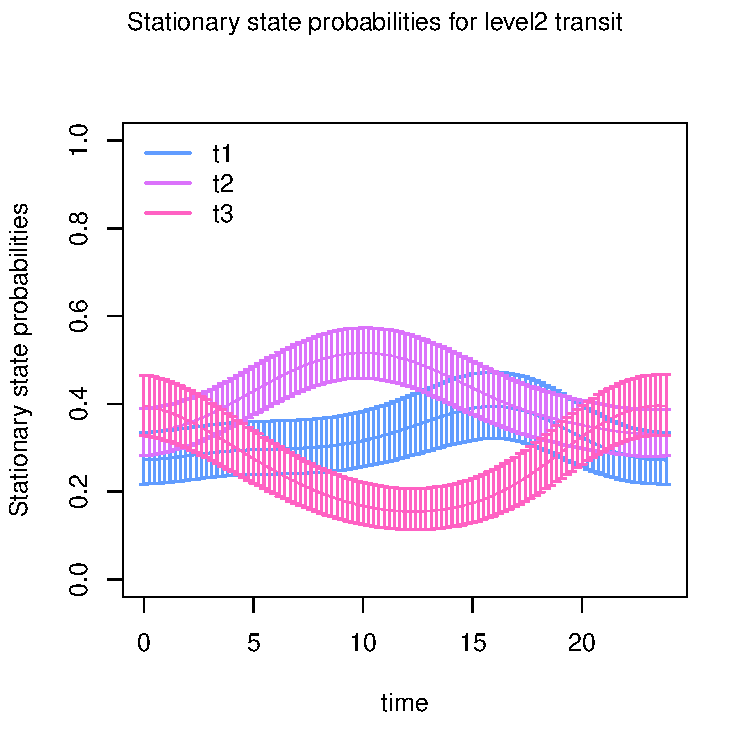
\includegraphics[width=.49\textwidth]{plot_codStationary003.pdf}
  \caption{Stationary distributions of the fine-scale state processes for an Atlantic cod as a function of time of day for the coarse-scale states corresponding to ``resting/foraging'' (top-left panel), ``mobile/foraging'' (top-right panel), and ``travelling/migrating'' (bottom panel).}
  \label{fig:codStat}
\end{figure}

\subsubsection{Horn shark}
\label{sec:hornShark}
For our final HHMM example, we'll quickly demonstrate how the horn shark example from \cite{AdamEtAl2019} can be fitted in \verb|momentuHMM|. The data streams in this example consist of coarse-scale categorical step lengths (\verb|stepCat|) based on estimated geopositions at 2 second intervals over 194 distinct segments and, within each 2 second interval, fine-scale accelerometer data that were summarized as 50 sequential values of overall dynamic body acceleration (\verb|odba|). The analysis included 8 categories for step length to construct a so-called histogram distribution of step lengths, where category 1 indicates zero step lengths and categories $2-8$ were defined by increasing cutoffs at 0.00075, 0.00125, 0.00175, 0.00225, 0.00275, 0.00325, and 0.00375 m, respectively. The 9-state HHMM included three coarse-scale states (``activity'', ``resting'', and ``transit''), each composed of three fine-scale states.

First we load and prepare the data \citep[available for download from][]{AdamEtAl2019}:

\begin{knitrout}
\definecolor{shadecolor}{rgb}{0.969, 0.969, 0.969}\color{fgcolor}\begin{kframe}
\begin{alltt}
\hlcom{# load the data from Adam et al }
\hlkwd{load}\hlstd{(}\hlstr{"horn_shark_data_set.RData"}\hlstd{)}
\end{alltt}
\end{kframe}
\end{knitrout}
\begin{knitrout}
\definecolor{shadecolor}{rgb}{0.969, 0.969, 0.969}\color{fgcolor}\begin{kframe}
\begin{alltt}
\hlcom{# coarse-scale data}
\hlstd{data} \hlkwb{<-} \hlkwd{data.frame}\hlstd{(}\hlkwc{ID}\hlstd{=}\hlkwd{unlist}\hlstd{(}\hlkwd{mapply}\hlstd{(}\hlkwa{function}\hlstd{(}\hlkwc{x}\hlstd{)} \hlkwd{rep}\hlstd{(}\hlkwd{paste0}\hlstd{(}\hlstr{"seg"}\hlstd{,x),}
                                                    \hlkwd{nrow}\hlstd{(steps[[x]])}\hlopt{-}\hlnum{1}\hlstd{),}
                                    \hlnum{1}\hlopt{:}\hlkwd{length}\hlstd{(steps))),}
                   \hlkwc{level}\hlstd{=}\hlstr{"1"}\hlstd{,}
                   \hlkwc{steps}\hlstd{=}\hlkwd{unlist}\hlstd{(}\hlkwd{lapply}\hlstd{(steps,}\hlkwa{function}\hlstd{(}\hlkwc{x}\hlstd{) x}\hlopt{$}\hlstd{steps[}\hlopt{-}\hlkwd{nrow}\hlstd{(x)])),}
                   \hlkwc{stepCat}\hlstd{=}\hlkwd{unlist}\hlstd{(}\hlkwd{lapply}\hlstd{(steps,}\hlkwa{function}\hlstd{(}\hlkwc{x}\hlstd{) x}\hlopt{$}\hlstd{cats[}\hlopt{-}\hlkwd{nrow}\hlstd{(x)])),}
                   \hlkwc{odbas}\hlstd{=}\hlnum{NA}\hlstd{)}
\hlstd{data}\hlopt{$}\hlstd{stepCat[}\hlkwd{which}\hlstd{(}\hlkwd{is.na}\hlstd{(data}\hlopt{$}\hlstd{steps))]} \hlkwb{<-} \hlnum{NA}

\hlcom{### add extra rows for fine-scale data}
\hlcom{# level=1  indicates when coarse-scale behavior switching can occur }
\hlcom{# level=2i indicates start of each fine-scale interval}
\hlcom{# level=2  indicates when fine-scale behavior switching can occur}
\hlstd{odbas} \hlkwb{<-} \hlkwd{unlist}\hlstd{(odbas)}
\hlstd{sharkData} \hlkwb{<-} \hlkwa{NULL}
\hlkwa{for}\hlstd{(i} \hlkwa{in} \hlnum{1}\hlopt{:}\hlkwd{nrow}\hlstd{(data))\{}
  \hlstd{fineInd} \hlkwb{<-} \hlkwd{data.frame}\hlstd{(}\hlkwc{ID}\hlstd{=data}\hlopt{$}\hlstd{ID[i],}
                        \hlkwc{level}\hlstd{=}\hlstr{"2"}\hlstd{,}
                        \hlkwc{steps}\hlstd{=}\hlnum{NA}\hlstd{,}
                        \hlkwc{stepCat}\hlstd{=}\hlnum{NA}\hlstd{,}
                        \hlkwc{odbas}\hlstd{=odbas[(i}\hlopt{-}\hlnum{1}\hlstd{)}\hlopt{*}\hlnum{50}\hlopt{+}\hlnum{1}\hlopt{:}\hlnum{50}\hlstd{])}
  \hlstd{tmp} \hlkwb{<-} \hlkwd{rbind}\hlstd{(data[i,,}\hlkwc{drop}\hlstd{=}\hlnum{FALSE}\hlstd{],}
               \hlkwd{data.frame}\hlstd{(}\hlkwc{ID}\hlstd{=data}\hlopt{$}\hlstd{ID[i],}
                          \hlkwc{level}\hlstd{=}\hlstr{"2i"}\hlstd{,}
                          \hlkwc{steps}\hlstd{=}\hlnum{NA}\hlstd{,}
                          \hlkwc{stepCat}\hlstd{=}\hlnum{NA}\hlstd{,}
                          \hlkwc{odbas}\hlstd{=}\hlnum{NA}\hlstd{),}
               \hlstd{fineInd)}
  \hlstd{sharkData} \hlkwb{<-} \hlkwd{rbind}\hlstd{(sharkData,tmp)}
\hlstd{\}}

\hlcom{# prepare hierarchical data}
\hlstd{sharkData} \hlkwb{<-} \hlkwd{prepData}\hlstd{(sharkData,}\hlkwc{coordNames}\hlstd{=}\hlkwa{NULL}\hlstd{,}
                      \hlkwc{hierLevels}\hlstd{=}\hlkwd{c}\hlstd{(}\hlstr{"1"}\hlstd{,}\hlstr{"2i"}\hlstd{,}\hlstr{"2"}\hlstd{))}
\hlkwd{head}\hlstd{(sharkData)}
\end{alltt}
\begin{verbatim}
##     ID level       steps stepCat      odbas
## 1 seg1     1 0.001447295       4         NA
## 2 seg1    2i          NA      NA         NA
## 3 seg1     2          NA      NA 0.07733020
## 4 seg1     2          NA      NA 0.07424251
## 5 seg1     2          NA      NA 0.07866384
## 6 seg1     2          NA      NA 0.07899367
\end{verbatim}
\end{kframe}
\end{knitrout}
\noindent Note that because the 194 segments were observed irregularly in bouts of time over the coarse of one night, \cite{AdamEtAl2019} essentially treated each segment as a different track whereby the HHMM ``resets'' at the beginning of each segment; this can be accomplished in \verb|momentuHMM| by simply assigning each segment its own \verb|ID| as was done above.

Next we define the hierarchical nature of the states and data streams:
\begin{knitrout}
\definecolor{shadecolor}{rgb}{0.969, 0.969, 0.969}\color{fgcolor}\begin{kframe}
\begin{alltt}
\hlcom{### define hierarchical HMM }
\hlcom{# states 1-3 = coarse state 1 (high activity)}
\hlcom{# states 4-6 = coarse state 2 (resting)}
\hlcom{# states 7-9 = coarse state 3 (travelling)}
\hlstd{hierStates} \hlkwb{<-} \hlstd{data.tree}\hlopt{::}\hlstd{Node}\hlopt{$}\hlkwd{new}\hlstd{(}\hlstr{"shark HHMM states"}\hlstd{)}
\hlstd{hierStates}\hlopt{$}\hlkwd{AddChild}\hlstd{(}\hlstr{"activity"}\hlstd{)} \hlcom{# zero distance travelled, high activity}
\hlstd{hierStates}\hlopt{$}\hlstd{activity}\hlopt{$}\hlkwd{AddChild}\hlstd{(}\hlstr{"a1"}\hlstd{,} \hlkwc{state}\hlstd{=}\hlnum{1}\hlstd{)}
\hlstd{hierStates}\hlopt{$}\hlstd{activity}\hlopt{$}\hlkwd{AddChild}\hlstd{(}\hlstr{"a2"}\hlstd{,} \hlkwc{state}\hlstd{=}\hlnum{2}\hlstd{)}
\hlstd{hierStates}\hlopt{$}\hlstd{activity}\hlopt{$}\hlkwd{AddChild}\hlstd{(}\hlstr{"a3"}\hlstd{,} \hlkwc{state}\hlstd{=}\hlnum{3}\hlstd{)}
\hlstd{hierStates}\hlopt{$}\hlkwd{AddChild}\hlstd{(}\hlstr{"resting"}\hlstd{)}  \hlcom{# zero distance travelled, low activity}
\hlstd{hierStates}\hlopt{$}\hlstd{resting}\hlopt{$}\hlkwd{AddChild}\hlstd{(}\hlstr{"r1"}\hlstd{,} \hlkwc{state}\hlstd{=}\hlnum{4}\hlstd{)}
\hlstd{hierStates}\hlopt{$}\hlstd{resting}\hlopt{$}\hlkwd{AddChild}\hlstd{(}\hlstr{"r2"}\hlstd{,} \hlkwc{state}\hlstd{=}\hlnum{5}\hlstd{)}
\hlstd{hierStates}\hlopt{$}\hlstd{resting}\hlopt{$}\hlkwd{AddChild}\hlstd{(}\hlstr{"r3"}\hlstd{,} \hlkwc{state}\hlstd{=}\hlnum{6}\hlstd{)}
\hlstd{hierStates}\hlopt{$}\hlkwd{AddChild}\hlstd{(}\hlstr{"transit"}\hlstd{)}  \hlcom{# travelling}
\hlstd{hierStates}\hlopt{$}\hlstd{transit}\hlopt{$}\hlkwd{AddChild}\hlstd{(}\hlstr{"t1"}\hlstd{,} \hlkwc{state}\hlstd{=}\hlnum{7}\hlstd{)}
\hlstd{hierStates}\hlopt{$}\hlstd{transit}\hlopt{$}\hlkwd{AddChild}\hlstd{(}\hlstr{"t2"}\hlstd{,} \hlkwc{state}\hlstd{=}\hlnum{8}\hlstd{)}
\hlstd{hierStates}\hlopt{$}\hlstd{transit}\hlopt{$}\hlkwd{AddChild}\hlstd{(}\hlstr{"t3"}\hlstd{,} \hlkwc{state}\hlstd{=}\hlnum{9}\hlstd{)}

\hlkwd{plot}\hlstd{(hierStates)}
\end{alltt}
\end{kframe}
\includegraphics[width=\maxwidth]{figure/shark-2-1} 
\begin{kframe}\begin{alltt}
\hlstd{nbStates} \hlkwb{<-} \hlkwd{length}\hlstd{(hierStates}\hlopt{$}\hlkwd{Get}\hlstd{(}\hlstr{"state"}\hlstd{,}\hlkwc{filterFun}\hlstd{=data.tree}\hlopt{::}\hlstd{isLeaf))}
\hlstd{nCat} \hlkwb{<-} \hlnum{8} \hlcom{# number of stepCat categories}

\hlcom{# data stream distributions }
\hlcom{# level 1 = coarse level (stepCat="cat8")}
\hlcom{# level 2 = fine level (odbas="gamma")}
\hlstd{hierDist} \hlkwb{<-} \hlstd{data.tree}\hlopt{::}\hlstd{Node}\hlopt{$}\hlkwd{new}\hlstd{(}\hlstr{"shark HHMM dist"}\hlstd{)}
\hlstd{hierDist}\hlopt{$}\hlkwd{AddChild}\hlstd{(}\hlstr{"level1"}\hlstd{)}
\hlstd{hierDist}\hlopt{$}\hlstd{level1}\hlopt{$}\hlkwd{AddChild}\hlstd{(}\hlstr{"stepCat"}\hlstd{,} \hlkwc{dist}\hlstd{=}\hlkwd{paste0}\hlstd{(}\hlstr{"cat"}\hlstd{,nCat))}
\hlstd{hierDist}\hlopt{$}\hlkwd{AddChild}\hlstd{(}\hlstr{"level2"}\hlstd{)}
\hlstd{hierDist}\hlopt{$}\hlstd{level2}\hlopt{$}\hlkwd{AddChild}\hlstd{(}\hlstr{"odbas"}\hlstd{,} \hlkwc{dist}\hlstd{=}\hlstr{"gamma"}\hlstd{)}

\hlkwd{plot}\hlstd{(hierDist)}
\end{alltt}
\end{kframe}
\includegraphics[width=\maxwidth]{figure/shark-2-2} 

\end{knitrout}
\noindent This is the first example in the vignette that uses a categorical data stream probability distribution, so it is perhaps worth describing this in a little more detail. When specifying categorical distributions, the number of categories must be indicated. In this case, there are 8 \verb|stepCat| categories, so we specify this as \verb|cat8|. Generally, categorical distributions are specified as \verb|paste0("cat",nCat)|, where \verb|nCat| is an integer greater than 2 (note that a categorical distribution with only 2 categories is simply a Bernoulli distribution). The categorical distribution parameters are \verb|nCat| probabilities that sum to 1, so the mlogit link is used and only \verb|nCat| $-1$ working parameters are estimated in order to obtain the \verb|nCat| categorical probabilities on the real scale.

Both the ``activity'' and ``resting'' coarse-scale states were assumed to have zero distance travelled (i.e., \verb|stepCat| $=1$), while the ``transit'' state was assumed to have $>0$ distance travelled (i.e., \verb|stepCat| $\in{2,\ldots,8}$). We therefore need to constrain the categorical step length probabilities for each fine-scale state within each coarse-scale state accordingly:
\begin{knitrout}
\definecolor{shadecolor}{rgb}{0.969, 0.969, 0.969}\color{fgcolor}\begin{kframe}
\begin{alltt}
\hlcom{### starting values based on Adam et al}
\hlstd{mu0} \hlkwb{<-} \hlkwd{c}\hlstd{(}\hlnum{0.191}\hlstd{,} \hlnum{0.323}\hlstd{,} \hlnum{0.721}\hlstd{,} \hlnum{0.084}\hlstd{,} \hlnum{0.15}\hlstd{,} \hlnum{0.228}\hlstd{,} \hlnum{0.094}\hlstd{,} \hlnum{0.191}\hlstd{,} \hlnum{0.39}\hlstd{)}
\hlstd{sd0} \hlkwb{<-} \hlkwd{c}\hlstd{(}\hlnum{0.047}\hlstd{,} \hlnum{0.051}\hlstd{,} \hlnum{0.248}\hlstd{,} \hlnum{0.021}\hlstd{,} \hlnum{0.025}\hlstd{,} \hlnum{0.033}\hlstd{,} \hlnum{0.026}\hlstd{,} \hlnum{0.039}\hlstd{,} \hlnum{0.159}\hlstd{)}
\hlstd{probs0} \hlkwb{<-} \hlkwd{c}\hlstd{(}\hlnum{1e+10}\hlstd{,} \hlopt{-}\hlnum{1e+10}\hlstd{,} \hlnum{0.958}\hlstd{,} \hlnum{5.064}\hlstd{,} \hlnum{3.261}\hlstd{,} \hlnum{4.021}\hlstd{,} \hlnum{0.473}\hlstd{,} \hlnum{2.568}\hlstd{)}

\hlcom{# constrain coarse-scale parameters for fine-scale states}
\hlstd{DM} \hlkwb{<-} \hlkwd{list}\hlstd{(}\hlkwc{stepCat}\hlstd{=}\hlkwd{matrix}\hlstd{(}\hlkwd{cbind}\hlstd{(}\hlkwd{c}\hlstd{(}\hlkwd{rep}\hlstd{(}\hlkwd{c}\hlstd{(}\hlnum{1}\hlstd{,}\hlnum{1}\hlstd{,}\hlnum{1}\hlstd{),}\hlnum{2}\hlstd{),}
                                  \hlkwd{rep}\hlstd{(}\hlnum{0}\hlstd{,(nCat}\hlopt{-}\hlnum{1}\hlstd{)}\hlopt{*}\hlstd{nbStates}\hlopt{-}\hlnum{6}\hlstd{)),}
                                \hlkwd{kronecker}\hlstd{(}\hlkwd{diag}\hlstd{(nCat}\hlopt{-}\hlnum{1}\hlstd{),}
                                          \hlkwd{c}\hlstd{(}\hlnum{0}\hlstd{,}\hlnum{0}\hlstd{,}\hlnum{0}\hlstd{,}\hlnum{0}\hlstd{,}\hlnum{0}\hlstd{,}\hlnum{0}\hlstd{,}\hlnum{1}\hlstd{,}\hlnum{1}\hlstd{,}\hlnum{1}\hlstd{))),}
                       \hlkwc{nrow}\hlstd{=(nCat}\hlopt{-}\hlnum{1}\hlstd{)}\hlopt{*}\hlstd{nbStates,}
                       \hlkwc{ncol}\hlstd{=}\hlnum{8}\hlstd{,}
                       \hlkwc{dimnames}\hlstd{=}\hlkwd{list}\hlstd{(}\hlkwd{paste0}\hlstd{(}\hlkwd{rep}\hlstd{(}\hlkwd{paste0}\hlstd{(}\hlstr{"prob"}\hlstd{,}
                                                       \hlnum{1}\hlopt{:}\hlstd{(nCat}\hlopt{-}\hlnum{1}\hlstd{),}
                                                       \hlstr{"_"}\hlstd{),}
                                                \hlkwc{each}\hlstd{=nbStates),}
                                            \hlnum{1}\hlopt{:}\hlstd{nbStates),}
                                     \hlkwd{c}\hlstd{(}\hlkwd{paste0}\hlstd{(}\hlkwd{c}\hlstd{(}\hlstr{"prob1_12"}\hlstd{,}
                                                \hlkwd{paste0}\hlstd{(}\hlstr{"prob"}\hlstd{,}
                                                       \hlnum{1}\hlopt{:}\hlstd{(nCat}\hlopt{-}\hlnum{1}\hlstd{),}
                                                       \hlstr{"_3"}\hlstd{)),}
                                              \hlstr{":(Intercept)"}\hlstd{)))))}
\hlkwd{head}\hlstd{(DM}\hlopt{$}\hlstd{stepCat,nbStates)}
\end{alltt}
\begin{verbatim}
##         prob1_12:(Intercept) prob1_3:(Intercept) prob2_3:(Intercept)
## prob1_1                    1                   0                   0
## prob1_2                    1                   0                   0
## prob1_3                    1                   0                   0
## prob1_4                    1                   0                   0
## prob1_5                    1                   0                   0
## prob1_6                    1                   0                   0
## prob1_7                    0                   1                   0
## prob1_8                    0                   1                   0
## prob1_9                    0                   1                   0
##         prob3_3:(Intercept) prob4_3:(Intercept) prob5_3:(Intercept)
## prob1_1                   0                   0                   0
## prob1_2                   0                   0                   0
## prob1_3                   0                   0                   0
## prob1_4                   0                   0                   0
## prob1_5                   0                   0                   0
## prob1_6                   0                   0                   0
## prob1_7                   0                   0                   0
## prob1_8                   0                   0                   0
## prob1_9                   0                   0                   0
##         prob6_3:(Intercept) prob7_3:(Intercept)
## prob1_1                   0                   0
## prob1_2                   0                   0
## prob1_3                   0                   0
## prob1_4                   0                   0
## prob1_5                   0                   0
## prob1_6                   0                   0
## prob1_7                   0                   0
## prob1_8                   0                   0
## prob1_9                   0                   0
\end{verbatim}
\begin{alltt}
\hlstd{Par0} \hlkwb{<-} \hlkwd{list}\hlstd{(}\hlkwc{stepCat} \hlstd{= probs0,}
             \hlkwc{odbas} \hlstd{=} \hlkwd{c}\hlstd{(mu0,sd0))}

\hlstd{fixPar} \hlkwb{<-} \hlkwd{list}\hlstd{(}\hlkwc{stepCat}\hlstd{=}\hlkwd{c}\hlstd{(}\hlnum{1.e+10}\hlstd{,}\hlopt{-}\hlnum{1.e+10}\hlstd{,}\hlkwd{rep}\hlstd{(}\hlnum{NA}\hlstd{,}\hlnum{6}\hlstd{)))}
\end{alltt}
\end{kframe}
\end{knitrout}
\noindent By fixing the working parameter corresponding to the probability of observing step length category 1 (\verb|prob1|) for coarse-scale state 1 (fine-scale states $1-3$) and coarse-scale state 2 (fine-scale states $4-6$) to a very large positive number, we have effectively fixed \verb|prob1| $=1$ for these states. Likewise, by fixing the working parameter corresponding to \verb|prob1| for coarse-scale state 3 (fine-scale states $7-9$) to a very large negative number, we have effectively fixed \verb|prob1| $=0$ for this state.

All that remains is (optionally) specifying starting values for the initial distribution (\verb|hierDelta|) and t.p.m. (\verb|hierBeta|) parameters, and let's check our model specification before fitting using \verb|checkPar0|:
\begin{knitrout}
\definecolor{shadecolor}{rgb}{0.969, 0.969, 0.969}\color{fgcolor}\begin{kframe}
\begin{alltt}
\hlcom{### t.p.m. starting values based on Adam et al}
\hlstd{hierBeta} \hlkwb{<-} \hlstd{data.tree}\hlopt{::}\hlstd{Node}\hlopt{$}\hlkwd{new}\hlstd{(}\hlstr{"shark beta"}\hlstd{)}
\hlstd{hierBeta}\hlopt{$}\hlkwd{AddChild}\hlstd{(}\hlstr{"level1"}\hlstd{,}
   \hlkwc{beta}\hlstd{=}\hlkwd{matrix}\hlstd{(}\hlkwd{c}\hlstd{(}\hlopt{-}\hlnum{0.651}\hlstd{,} \hlopt{-}\hlnum{0.169}\hlstd{,} \hlopt{-}\hlnum{1.884}\hlstd{,} \hlopt{-}\hlnum{0.369}\hlstd{,} \hlopt{-}\hlnum{1.596}\hlstd{,} \hlopt{-}\hlnum{0.737}\hlstd{),}
               \hlkwc{ncol}\hlstd{=}\hlkwd{length}\hlstd{(hierStates}\hlopt{$}\hlstd{children)}
                    \hlopt{*}\hlstd{(}\hlkwd{length}\hlstd{(hierStates}\hlopt{$}\hlstd{children)}\hlopt{-}\hlnum{1}\hlstd{)))}
\hlstd{hierBeta}\hlopt{$}\hlkwd{AddChild}\hlstd{(}\hlstr{"level2"}\hlstd{)}
\hlstd{hierBeta}\hlopt{$}\hlstd{level2}\hlopt{$}\hlkwd{AddChild}\hlstd{(}\hlstr{"activity"}\hlstd{,}
   \hlkwc{beta}\hlstd{=}\hlkwd{matrix}\hlstd{(}\hlkwd{c}\hlstd{(}\hlopt{-}\hlnum{2.902}\hlstd{,} \hlopt{-}\hlnum{14.032}\hlstd{,} \hlnum{3.059}\hlstd{,} \hlopt{-}\hlnum{1.37}\hlstd{,} \hlnum{8.098}\hlstd{,} \hlnum{11.66}\hlstd{),}
               \hlkwc{ncol}\hlstd{=}\hlkwd{length}\hlstd{(hierStates}\hlopt{$}\hlstd{activity}\hlopt{$}\hlstd{children)}
                    \hlopt{*}\hlstd{(}\hlkwd{length}\hlstd{(hierStates}\hlopt{$}\hlstd{activity}\hlopt{$}\hlstd{children)}\hlopt{-}\hlnum{1}\hlstd{)))}
\hlstd{hierBeta}\hlopt{$}\hlstd{level2}\hlopt{$}\hlkwd{AddChild}\hlstd{(}\hlstr{"resting"}\hlstd{,}
   \hlkwc{beta}\hlstd{=}\hlkwd{matrix}\hlstd{(}\hlkwd{c}\hlstd{(}\hlopt{-}\hlnum{3.264}\hlstd{,} \hlopt{-}\hlnum{14.279}\hlstd{,} \hlnum{3.107}\hlstd{,} \hlnum{0.252}\hlstd{,} \hlnum{13.861}\hlstd{,} \hlnum{16.468}\hlstd{),}
               \hlkwc{ncol}\hlstd{=}\hlkwd{length}\hlstd{(hierStates}\hlopt{$}\hlstd{resting}\hlopt{$}\hlstd{children)}
                    \hlopt{*}\hlstd{(}\hlkwd{length}\hlstd{(hierStates}\hlopt{$}\hlstd{resting}\hlopt{$}\hlstd{children)}\hlopt{-}\hlnum{1}\hlstd{)))}
\hlstd{hierBeta}\hlopt{$}\hlstd{level2}\hlopt{$}\hlkwd{AddChild}\hlstd{(}\hlstr{"transit"}\hlstd{,}
   \hlkwc{beta}\hlstd{=}\hlkwd{matrix}\hlstd{(}\hlkwd{c}\hlstd{(}\hlopt{-}\hlnum{3.21}\hlstd{,} \hlopt{-}\hlnum{21.32}\hlstd{,} \hlnum{3.463}\hlstd{,} \hlopt{-}\hlnum{0.598}\hlstd{,} \hlnum{14.636}\hlstd{,} \hlnum{17.811}\hlstd{),}
               \hlkwc{ncol}\hlstd{=}\hlkwd{length}\hlstd{(hierStates}\hlopt{$}\hlstd{transit}\hlopt{$}\hlstd{children)}
                    \hlopt{*}\hlstd{(}\hlkwd{length}\hlstd{(hierStates}\hlopt{$}\hlstd{transit}\hlopt{$}\hlstd{children)}\hlopt{-}\hlnum{1}\hlstd{)))}

\hlcom{### initial distribution starting values based on Adam et al}
\hlstd{hierDelta} \hlkwb{<-} \hlstd{data.tree}\hlopt{::}\hlstd{Node}\hlopt{$}\hlkwd{new}\hlstd{(}\hlstr{"shark delta"}\hlstd{)}
\hlstd{hierDelta}\hlopt{$}\hlkwd{AddChild}\hlstd{(}\hlstr{"level1"}\hlstd{,}
   \hlkwc{delta}\hlstd{=}\hlkwd{matrix}\hlstd{(}\hlkwd{c}\hlstd{(}\hlnum{0.582}\hlstd{,} \hlnum{2.894}\hlstd{),}
                \hlkwc{ncol}\hlstd{=}\hlkwd{length}\hlstd{(hierStates}\hlopt{$}\hlstd{children)}\hlopt{-}\hlnum{1}\hlstd{))}
\hlstd{hierDelta}\hlopt{$}\hlkwd{AddChild}\hlstd{(}\hlstr{"level2"}\hlstd{)}
\hlstd{hierDelta}\hlopt{$}\hlstd{level2}\hlopt{$}\hlkwd{AddChild}\hlstd{(}\hlstr{"activity"}\hlstd{,}
   \hlkwc{delta}\hlstd{=}\hlkwd{matrix}\hlstd{(}\hlkwd{c}\hlstd{(}\hlopt{-}\hlnum{0.001}\hlstd{,} \hlopt{-}\hlnum{1.1}\hlstd{),}
                \hlkwc{ncol}\hlstd{=}\hlkwd{length}\hlstd{(hierStates}\hlopt{$}\hlstd{activity}\hlopt{$}\hlstd{children)}\hlopt{-}\hlnum{1}\hlstd{))}
\hlstd{hierDelta}\hlopt{$}\hlstd{level2}\hlopt{$}\hlkwd{AddChild}\hlstd{(}\hlstr{"resting"}\hlstd{,}
   \hlkwc{delta}\hlstd{=}\hlkwd{matrix}\hlstd{(}\hlkwd{c}\hlstd{(}\hlopt{-}\hlnum{0.103}\hlstd{,} \hlopt{-}\hlnum{0.105}\hlstd{),}
                \hlkwc{ncol}\hlstd{=}\hlkwd{length}\hlstd{(hierStates}\hlopt{$}\hlstd{resting}\hlopt{$}\hlstd{children)}\hlopt{-}\hlnum{1}\hlstd{))}
\hlstd{hierDelta}\hlopt{$}\hlstd{level2}\hlopt{$}\hlkwd{AddChild}\hlstd{(}\hlstr{"transit"}\hlstd{,}
   \hlkwc{delta}\hlstd{=}\hlkwd{matrix}\hlstd{(}\hlkwd{c}\hlstd{(}\hlnum{0.24}\hlstd{,} \hlopt{-}\hlnum{0.777}\hlstd{),}
                \hlkwc{ncol}\hlstd{=}\hlkwd{length}\hlstd{(hierStates}\hlopt{$}\hlstd{transit}\hlopt{$}\hlstd{children)}\hlopt{-}\hlnum{1}\hlstd{))}

\hlcom{# check hierarchical model specification and parameters}
\hlkwd{checkPar0}\hlstd{(sharkData,}
          \hlkwc{hierStates}\hlstd{=hierStates,}
          \hlkwc{hierDist}\hlstd{=hierDist,}
          \hlkwc{Par0}\hlstd{=Par0,}
          \hlkwc{DM}\hlstd{=DM,}
          \hlkwc{hierBeta}\hlstd{=hierBeta,}
          \hlkwc{hierDelta}\hlstd{=hierDelta,}
          \hlkwc{fixPar}\hlstd{=fixPar)}
\end{alltt}
\begin{verbatim}
## 
## Regression coeffs for stepCat parameters:
## -----------------------------------------
##      prob1_12:(Intercept) prob1_3:(Intercept) prob2_3:(Intercept)
## [1,]                1e+10              -1e+10               0.958
##      prob3_3:(Intercept) prob4_3:(Intercept) prob5_3:(Intercept)
## [1,]               5.064               3.261               4.021
##      prob6_3:(Intercept) prob7_3:(Intercept)
## [1,]               0.473               2.568
## 
## odbas parameters:
## -----------------
##         a1    a2    a3    r1    r2    r3    t1    t2    t3
## mean 0.191 0.323 0.721 0.084 0.150 0.228 0.094 0.191 0.390
## sd   0.047 0.051 0.248 0.021 0.025 0.033 0.026 0.039 0.159
## 
## ----------------------------------------------------------
## Regression coeffs for the transition probabilities (beta):
## ----------------------------------------------------------
## -------------------------  level1  -----------------------
##                       1 -> 4 1 -> 7 4 -> 1 4 -> 7 7 -> 1 7 -> 4
## I((level == "1") * 1) -0.651 -0.169 -1.884 -0.369 -1.596 -0.737
## 
## -------------------------  level2  -----------------------
##                       1 -> 2  1 -> 3 2 -> 2 2 -> 3 3 -> 2 3 -> 3
## I((level == "2") * 1) -2.902 -14.032  3.059  -1.37  8.098  11.66
## 
##                       4 -> 5  4 -> 6 5 -> 5 5 -> 6 6 -> 5 6 -> 6
## I((level == "2") * 1) -3.264 -14.279  3.107  0.252 13.861 16.468
## 
##                       7 -> 8 7 -> 9 8 -> 8 8 -> 9 9 -> 8 9 -> 9
## I((level == "2") * 1)  -3.21 -21.32  3.463 -0.598 14.636 17.811
## 
## ----------------------------------------------------------
## 
## ----------------------------------------------------------
## Regression coeffs for the initial distribution (delta):
## ----------------------------------------------------------
## ------------------------  level1  ------------------------
##             state 4 state 7
## (Intercept)   0.582   2.894
## 
## ------------------------  level2  ------------------------
##                        state 2 state 3
## I((level == "2i") * 1)  -0.001    -1.1
## 
##                        state 5 state 6
## I((level == "2i") * 1)  -0.103  -0.105
## 
##                        state 8 state 9
## I((level == "2i") * 1)    0.24  -0.777
## 
## ----------------------------------------------------------
\end{verbatim}
\end{kframe}
\end{knitrout}
\noindent Everything checks out, so let's now fit the horn shark HHMM:
\begin{knitrout}
\definecolor{shadecolor}{rgb}{0.969, 0.969, 0.969}\color{fgcolor}\begin{kframe}
\begin{alltt}
\hlstd{hhmm} \hlkwb{<-} \hlkwd{fitHMM}\hlstd{(sharkData,}
               \hlkwc{hierStates}\hlstd{=hierStates,}
               \hlkwc{hierDist}\hlstd{=hierDist,}
               \hlkwc{Par0}\hlstd{=Par0,}
               \hlkwc{hierBeta}\hlstd{=hierBeta,}
               \hlkwc{hierDelta}\hlstd{=hierDelta,}
               \hlkwc{DM}\hlstd{=DM,}
               \hlkwc{fixPar}\hlstd{=fixPar)}

\hlcom{# transition probabilities for level1 and level2}
\hlstd{trProbs12} \hlkwb{<-} \hlkwd{getTrProbs}\hlstd{(hhmm,} \hlkwc{covIndex}\hlstd{=}\hlkwd{c}\hlstd{(}\hlnum{1}\hlstd{,}\hlnum{3}\hlstd{))}

\hlcom{# stationary distributions for level1 and level2}
\hlstd{stats12} \hlkwb{<-} \hlkwd{stationary}\hlstd{(hhmm,} \hlkwc{covIndex}\hlstd{=}\hlkwd{c}\hlstd{(}\hlnum{1}\hlstd{,}\hlnum{3}\hlstd{))}
\end{alltt}
\end{kframe}
\end{knitrout}
The resulting estimates are again very similar to \cite{AdamEtAl2019}, with the slight differences attributable to \cite{AdamEtAl2019} assuming the initial distributions for each level of the hierarchy are equal to the stationary distributions. Nevertheless, we can see that the estimated t.p.m. and stationary distributions are very similar:
\begin{knitrout}
\definecolor{shadecolor}{rgb}{0.969, 0.969, 0.969}\color{fgcolor}\begin{kframe}
\begin{alltt}
\hlcom{### coarse scale #####################################}
\hlcom{# t.p.m.}
\hlkwd{round}\hlstd{(trProbs12}\hlopt{$}\hlstd{level1}\hlopt{$}\hlstd{gamma[,,}\hlnum{1}\hlstd{],}\hlnum{3}\hlstd{)}
\end{alltt}
\begin{verbatim}
##          activity resting transit
## activity    0.423   0.221   0.357
## resting     0.082   0.543   0.375
## transit     0.121   0.285   0.594
\end{verbatim}
\begin{alltt}
\hlcom{# stationary distribution}
\hlkwd{round}\hlstd{(stats12[[}\hlnum{1}\hlstd{]]}\hlopt{$}\hlstd{level1[}\hlnum{1}\hlstd{,],}\hlnum{3}\hlstd{)}
\end{alltt}
\begin{verbatim}
## activity  resting  transit 
##    0.153    0.371    0.477
\end{verbatim}
\begin{alltt}
\hlcom{######################################################}

\hlcom{### fine scale #######################################}
\hlcom{# t.p.m.}
\hlkwd{lapply}\hlstd{(trProbs12}\hlopt{$}\hlstd{level2,}\hlkwa{function}\hlstd{(}\hlkwc{x}\hlstd{)} \hlkwd{round}\hlstd{(x}\hlopt{$}\hlstd{gamma[,,}\hlnum{1}\hlstd{],}\hlnum{3}\hlstd{))}
\end{alltt}
\begin{verbatim}
## $activity
##       a1    a2    a3
## a1 0.948 0.052 0.000
## a2 0.044 0.944 0.011
## a3 0.000 0.028 0.972
## 
## $resting
##       r1    r2    r3
## r1 0.963 0.037 0.000
## r2 0.041 0.907 0.052
## r3 0.000 0.069 0.931
## 
## $transit
##       t1    t2    t3
## t1 0.961 0.039 0.000
## t2 0.030 0.954 0.016
## t3 0.000 0.040 0.960
\end{verbatim}
\begin{alltt}
\hlcom{# stationary distribution}
\hlkwd{lapply}\hlstd{(stats12[[}\hlnum{1}\hlstd{]]}\hlopt{$}\hlstd{level2,}\hlkwa{function}\hlstd{(}\hlkwc{x}\hlstd{)} \hlkwd{round}\hlstd{(x[}\hlnum{1}\hlstd{,],}\hlnum{3}\hlstd{))}
\end{alltt}
\begin{verbatim}
## $activity
##    a1    a2    a3 
## 0.377 0.443 0.181 
## 
## $resting
##    r1    r2    r3 
## 0.385 0.349 0.265 
## 
## $transit
##    t1    t2    t3 
## 0.353 0.459 0.188
\end{verbatim}
\begin{alltt}
\hlcom{######################################################}
\end{alltt}
\end{kframe}
\end{knitrout}

\subsection{African buffalo recharge dynamics}
\label{sec:buffalo}
Here we demonstrate how to fit a discrete-time version of the African buffalo recharge dynamics model from \cite{HootenEtAl2019} based only on surface water covariates. It is believed that water resources can strongly influence African buffalo space use, and surface water was therefore included in both the movement model (as distance to nearest surface water $d$) and the recharge function (as an indicator for being $<0.5$ km to nearest surface water $w$). The model includes $N=2$ states, where state 1 is the ``recharged'' state and state 2 is the ``discharged'' state. Conditional on the state $S_t \in \{1,2\}$, the discrete-time analogue to the continuous-time model of \cite{HootenEtAl2019} has the following bivariate normal random walk movement model for the locations $({\boldsymbol \mu}=(\mu_x,\mu_y))$ at time $t$:
\begin{equation*}
  {\boldsymbol \mu}_t \mid S_t=s \sim \mathcal{N}\left( {\boldsymbol \mu}_{t-1}+D({\boldsymbol \mu}_{t-1}){\boldsymbol \beta}^\mu I(s=2),\sigma_s^2 {\mathbf I} \right),
\end{equation*}
where $I()$ is the indicator function, $\mathbf I$ is a $2 \times 2$ identity matrix, and $D({\boldsymbol \mu}_t)$ is the negative gradient of $d$ evaluated at location ${\boldsymbol \mu}_t$. %$-\left(\frac{\partial d}{\partial x}, \frac{\partial d}{\partial y}\right)$
Thus when the animal is in the charged state (i.e. $S_t=1$), the movement model is a simple random walk. When the animal is in the discharged state (i.e. $S_t=2$), the movement model includes a potential function surface based on distance to nearest surface water \citep[for more on potential functions see][and sections \ref{sec:turtle} and \ref{sec:avoidLand}]{BrillingerEtAl2012,HootenEtAl2017,HootenEtAl2019}. In terms of $\Gamma^{(t)}$, the model for the state-switching dynamics is simply:
\begin{equation}
  {\mathbf \Gamma^{(t)}} = \begin{bmatrix}
    \frac{1}{(1+\exp(-g_t))} & \frac{\exp(-g_t)}{(1+\exp(-g_t))}  \\
    \frac{1}{(1+\exp(-g_t))} & \frac{\exp(-g_t)}{(1+\exp(-g_t))} 
  \end{bmatrix},
  \label{eq:rechargeTPM1}
\end{equation}
with recharge function
\begin{equation*}
  g_t = g_0 + \sum_{j=1}^t \theta_0 + w_j \theta_1,
\end{equation*}
where $w_j$ is the distance to nearest water indicator covariate at location ${\boldsymbol \mu}_j$. Thus the probability of being in the ``discharged'' state decreases as the recharge function $(g_t)$ increases. Note that there are no t.p.m. working parameter coefficients in Eq. \ref{eq:rechargeTPM1} and, because $\gamma_{11}=\gamma_{21}$ and $\gamma_{12}=\gamma_{22}$, the state switching in this model is not Markov (i.e., the state at time $t$ does not depend on the state at time $t-1$). 

In order to fit this model, we must first load the data and format the covariate rasters:
\begin{knitrout}
\definecolor{shadecolor}{rgb}{0.969, 0.969, 0.969}\color{fgcolor}\begin{kframe}
\begin{alltt}
\hlkwd{library}\hlstd{(raster)}

\hlcom{## download buffalo data}
\hlkwd{load}\hlstd{(}\hlkwd{url}\hlstd{(}\hlkwd{paste0}\hlstd{(}\hlstr{"https://github.com/henryrscharf/"}\hlstd{,}
         \hlstr{"Hooten_et_al_EL_2018/raw/master/"}\hlstd{,}
         \hlstr{"data/buffalo/buffalo_Cilla.RData"}\hlstd{)))}

\hlcom{## download distance to water covariate raster}
\hlkwd{load}\hlstd{(}\hlkwd{url}\hlstd{(}\hlkwd{paste0}\hlstd{(}\hlstr{"https://github.com/henryrscharf/"}\hlstd{,}
                \hlstr{"Hooten_et_al_EL_2018/raw/master/"}\hlstd{,}
                \hlstr{"data/buffalo/dist2sabie.RData"}\hlstd{)))}
\hlkwd{names}\hlstd{(dist2sabie)} \hlkwb{<-} \hlstr{"dist2sabie"}

\hlcom{## standardize dist2sabie based on slope of gradient}
\hlstd{dist2sabie_scaled} \hlkwb{<-} \hlstd{dist2sabie} \hlopt{/} \hlkwd{mean}\hlstd{(}\hlkwd{values}\hlstd{(}\hlkwd{terrain}\hlstd{(dist2sabie,}
                                                      \hlkwc{opt} \hlstd{=} \hlstr{"slope"}\hlstd{)),}
                                       \hlkwc{na.rm} \hlstd{= T)}

\hlcom{# calculate gradient}
\hlstd{D_scaled} \hlkwb{<-} \hlstd{ctmcmove}\hlopt{::}\hlkwd{rast.grad}\hlstd{(dist2sabie_scaled)}

\hlcom{## W (recharge function covariates)}
\hlcom{# near_sabie = indicator for <500m from water}
\hlstd{intercept} \hlkwb{<-} \hlkwd{raster}\hlstd{(dist2sabie)}
\hlkwd{values}\hlstd{(intercept)} \hlkwb{<-} \hlnum{1}
\hlstd{W} \hlkwb{<-} \hlkwd{stack}\hlstd{(}\hlkwd{list}\hlstd{(}\hlstr{"intercept"} \hlstd{= intercept,}
                \hlstr{"near_sabie"} \hlstd{= dist2sabie} \hlopt{<} \hlnum{0.5e3}\hlstd{))}
\hlstd{W_names} \hlkwb{<-} \hlkwd{names}\hlstd{(W)}

\hlcom{## orthogonalize W based on locations ----}
\hlstd{W_ortho} \hlkwb{<-} \hlstd{W}
\hlstd{W_path} \hlkwb{<-} \hlkwd{extract}\hlstd{(}\hlkwc{x} \hlstd{= W,} \hlkwc{y} \hlstd{=} \hlkwd{matrix}\hlstd{(buffalo_proj}\hlopt{@}\hlkwc{coords}\hlstd{,} \hlkwc{ncol} \hlstd{=} \hlnum{2}\hlstd{))}
\hlstd{obstimes} \hlkwb{<-} \hlkwd{as.numeric}\hlstd{(buffalo_proj}\hlopt{$}\hlstd{POSIX)} \hlopt{/} \hlnum{3600} \hlcom{# numeric hours}
\hlstd{W_tilde} \hlkwb{<-} \hlkwd{apply}\hlstd{(W_path} \hlopt{*} \hlkwd{c}\hlstd{(}\hlnum{0}\hlstd{,} \hlkwd{diff}\hlstd{(obstimes)),} \hlnum{2}\hlstd{, cumsum)}
\hlstd{W_tilde_svd} \hlkwb{<-} \hlkwd{svd}\hlstd{(W_tilde)}
\hlstd{W_tilde_proj_mat} \hlkwb{<-} \hlstd{W_tilde_svd}\hlopt{$}\hlstd{v} \hlopt \hlkwd{diag}\hlstd{(W_tilde_svd}\hlopt{$}\hlstd{d}\hlopt{^}\hlstd{(}\hlopt{-}\hlnum{1}\hlstd{))}
\hlstd{W_mat} \hlkwb{<-} \hlkwd{as.matrix}\hlstd{(W)}
\hlstd{W_mat_proj} \hlkwb{<-} \hlstd{W_mat} \hlopt \hlstd{W_tilde_proj_mat}
\hlkwa{for}\hlstd{(layer} \hlkwa{in} \hlnum{1}\hlopt{:}\hlkwd{ncol}\hlstd{(W_mat))\{}
  \hlkwd{values}\hlstd{(W_ortho[[layer]])} \hlkwb{<-} \hlstd{W_mat_proj[, layer]}
  \hlkwd{names}\hlstd{(W_ortho[[layer]])} \hlkwb{<-} \hlkwd{paste0}\hlstd{(}\hlstr{"svd"}\hlstd{, layer)}
\hlstd{\}}
\end{alltt}
\end{kframe}
\end{knitrout}
\noindent Note that to (presumably) help with numerical stability, \cite{HootenEtAl2019} orthogonalized the recharge function covariates as above; the resulting recharge function is now $g_t = g_0 + \sum_{j=1}^t w^*_{1,j} \theta_1 + w^*_{2,j} \theta_2$, where $w^*_{1,j}$ and $w^*_{2,j}$ are the transformed intercept and distance indicator covariates, respectively.

The buffalo track data were collected from a GPS collar, but the roughly hourly observations were not perfectly regular.% (Figure \ref{fig:buffaloData}). 
%\begin{figure}[htbp]
%  \centering
%  \includegraphics[width=\textwidth]{plot_buffaloData.pdf}
%  \caption{Observed African buffalo locations relative to the distance to nearest surface water raster covariate (``dist2sabie'').}
%  \label{fig:buffaloData}
%\end{figure}
We will therefore use \verb|crawlWrap| to predict the track at regular 15 min intervals \citep[the average interval used by][]{HootenEtAl2019} and assume a conservative 50 m isotropic error ellipse for the measurement error model.
\begin{knitrout}
\definecolor{shadecolor}{rgb}{0.969, 0.969, 0.969}\color{fgcolor}\begin{kframe}
\begin{alltt}
\hlstd{lnError} \hlkwb{<-} \hlstd{crawl}\hlopt{::}\hlkwd{argosDiag2Cov}\hlstd{(}\hlnum{50}\hlstd{,}\hlnum{50}\hlstd{,}\hlnum{0}\hlstd{)} \hlcom{# 50m isotropic error ellipse}
\hlstd{buffaloData} \hlkwb{<-} \hlkwd{data.frame}\hlstd{(}\hlkwc{ID} \hlstd{=} \hlnum{1}\hlstd{,}
                          \hlkwc{time} \hlstd{= obstimes,}
                          \hlkwc{x} \hlstd{= buffalo_proj}\hlopt{@}\hlkwc{coords}\hlstd{[,} \hlnum{1}\hlstd{],}
                          \hlkwc{y} \hlstd{= buffalo_proj}\hlopt{@}\hlkwc{coords}\hlstd{[,} \hlnum{2}\hlstd{],}
                          \hlkwc{ln.sd.x} \hlstd{= lnError}\hlopt{$}\hlstd{ln.sd.x,}
                          \hlkwc{ln.sd.y} \hlstd{= lnError}\hlopt{$}\hlstd{ln.sd.y,}
                          \hlkwc{error.corr} \hlstd{= lnError}\hlopt{$}\hlstd{error.corr)}

\hlstd{crwOut} \hlkwb{<-} \hlkwd{crawlWrap}\hlstd{(buffaloData,}
                    \hlkwc{theta} \hlstd{=} \hlkwd{c}\hlstd{(}\hlnum{6.5}\hlstd{,}\hlopt{-}\hlnum{.1}\hlstd{),}
                    \hlkwc{fixPar} \hlstd{=} \hlkwd{c}\hlstd{(}\hlnum{1}\hlstd{,}\hlnum{1}\hlstd{,}\hlnum{NA}\hlstd{,}\hlnum{NA}\hlstd{),}
                    \hlkwc{err.model} \hlstd{=} \hlkwd{list}\hlstd{(}\hlkwc{x} \hlstd{=} \hlopt{~}\hlstd{ln.sd.x}\hlopt{-}\hlnum{1}\hlstd{,}
                                     \hlkwc{y} \hlstd{=} \hlopt{~}\hlstd{ln.sd.y}\hlopt{-}\hlnum{1}\hlstd{,}
                                     \hlkwc{rho} \hlstd{=} \hlopt{~}\hlstd{error.corr),}
                    \hlkwc{timeStep} \hlstd{=} \hlnum{0.25}\hlstd{,} \hlcom{# predict at 15 min time steps}
                    \hlkwc{attempts} \hlstd{=} \hlnum{10}\hlstd{)}
\end{alltt}
\end{kframe}
\end{knitrout}

Now we're ready to specify the recharge model. We'll first fit the model to the best predicted track from \verb|crawlWrap| and then use this model fit to specify starting values for a multiple imputation analysis:
\begin{knitrout}
\definecolor{shadecolor}{rgb}{0.969, 0.969, 0.969}\color{fgcolor}\begin{kframe}
\begin{alltt}
\hlstd{spatialCovs} \hlkwb{<-} \hlkwd{list}\hlstd{(}\hlkwc{W_intercept} \hlstd{= W_ortho}\hlopt{$}\hlstd{svd1,}
                    \hlkwc{W_near_sabie} \hlstd{= W_ortho}\hlopt{$}\hlstd{svd2,}
                    \hlkwc{dist2sabie} \hlstd{= dist2sabie,}
                    \hlkwc{D.x} \hlstd{= D_scaled}\hlopt{$}\hlstd{rast.grad.x,}
                    \hlkwc{D.y} \hlstd{= D_scaled}\hlopt{$}\hlstd{rast.grad.y)}

\hlcom{# best predicted track data}
\hlstd{hmmData} \hlkwb{<-} \hlkwd{prepData}\hlstd{(crwOut,}
                    \hlkwc{spatialCovs} \hlstd{= spatialCovs,}
                    \hlkwc{altCoordNames} \hlstd{=} \hlstr{"mu"}\hlstd{)}
\hlkwd{head}\hlstd{(hmmData[,}\hlkwd{c}\hlstd{(}\hlstr{"ID"}\hlstd{,}\hlstr{"time"}\hlstd{,} \hlstr{"mu.x"}\hlstd{,} \hlstr{"mu.y"}\hlstd{,}
                \hlstr{"W_intercept"}\hlstd{,}\hlstr{"W_near_sabie"}\hlstd{,}\hlstr{"dist2sabie"}\hlstd{,}
                \hlstr{"D.x"}\hlstd{,}\hlstr{"D.y"}\hlstd{)])}
\end{alltt}
\begin{verbatim}
##   ID     time     mu.x     mu.y   W_intercept W_near_sabie dist2sabie
## 1  1 313344.4 384560.8 -2770752 -0.0001873081 -0.003616337   1323.424
## 2  1 313344.7 384560.2 -2770750 -0.0001873081 -0.003616337   1323.424
## 3  1 313344.9 384559.7 -2770749 -0.0001873081 -0.003616337   1323.424
## 4  1 313345.2 384559.3 -2770747 -0.0001873081 -0.003616337   1323.424
## 5  1 313345.4 384559.1 -2770744 -0.0001873081 -0.003616337   1323.424
## 6  1 313345.7 384559.1 -2770742 -0.0001873081 -0.003616337   1323.424
##          D.x       D.y
## 1 -0.8709203 0.2576337
## 2 -0.8709203 0.2576337
## 3 -0.8709203 0.2576337
## 4 -0.8709203 0.2576337
## 5 -0.8709203 0.2576337
## 6 -0.8709203 0.2576337
\end{verbatim}
\begin{alltt}
\hlstd{nbStates} \hlkwb{<-} \hlnum{2}
\hlstd{stateNames} \hlkwb{<-} \hlkwd{c}\hlstd{(}\hlstr{"charged"}\hlstd{,} \hlstr{"discharged"}\hlstd{)}
\hlstd{dist} \hlkwb{<-} \hlkwd{list}\hlstd{(}\hlkwc{mu} \hlstd{=} \hlstr{"rw_mvnorm2"}\hlstd{)} \hlcom{# bivariate normal random walk}

\hlcom{# pseudo-design matrix for mu}
\hlstd{DM} \hlkwb{<-} \hlkwd{list}\hlstd{(}\hlkwc{mu}\hlstd{=}\hlkwd{matrix}\hlstd{(}\hlkwd{c}\hlstd{(}\hlstr{"mu.x_tm1"}\hlstd{,}         \hlnum{0}\hlstd{,}    \hlnum{0}\hlstd{,}\hlnum{0}\hlstd{,}\hlnum{0}\hlstd{,}\hlnum{0}\hlstd{,}
                       \hlstr{"mu.x_tm1"}\hlstd{,}         \hlnum{0}\hlstd{,}\hlstr{"D.x"}\hlstd{,}\hlnum{0}\hlstd{,}\hlnum{0}\hlstd{,}\hlnum{0}\hlstd{,}
                                \hlnum{0}\hlstd{,}\hlstr{"mu.y_tm1"}\hlstd{,}    \hlnum{0}\hlstd{,}\hlnum{0}\hlstd{,}\hlnum{0}\hlstd{,}\hlnum{0}\hlstd{,}
                                \hlnum{0}\hlstd{,}\hlstr{"mu.y_tm1"}\hlstd{,}\hlstr{"D.y"}\hlstd{,}\hlnum{0}\hlstd{,}\hlnum{0}\hlstd{,}\hlnum{0}\hlstd{,}
                                \hlnum{0}\hlstd{,}         \hlnum{0}\hlstd{,}    \hlnum{0}\hlstd{,}\hlnum{1}\hlstd{,}\hlnum{0}\hlstd{,}\hlnum{0}\hlstd{,}
                                \hlnum{0}\hlstd{,}         \hlnum{0}\hlstd{,}    \hlnum{0}\hlstd{,}\hlnum{0}\hlstd{,}\hlnum{1}\hlstd{,}\hlnum{0}\hlstd{,}
                                \hlnum{0}\hlstd{,}         \hlnum{0}\hlstd{,}    \hlnum{0}\hlstd{,}\hlnum{0}\hlstd{,}\hlnum{0}\hlstd{,}\hlnum{1}\hlstd{,}
                                \hlnum{0}\hlstd{,}         \hlnum{0}\hlstd{,}    \hlnum{0}\hlstd{,}\hlnum{0}\hlstd{,}\hlnum{0}\hlstd{,}\hlnum{1}\hlstd{,}
                                \hlnum{0}\hlstd{,}         \hlnum{0}\hlstd{,}    \hlnum{0}\hlstd{,}\hlnum{1}\hlstd{,}\hlnum{0}\hlstd{,}\hlnum{0}\hlstd{,}
                                \hlnum{0}\hlstd{,}         \hlnum{0}\hlstd{,}    \hlnum{0}\hlstd{,}\hlnum{0}\hlstd{,}\hlnum{1}\hlstd{,}\hlnum{0}\hlstd{),}
                     \hlnum{5}\hlopt{*}\hlstd{nbStates,}
                     \hlnum{6}\hlstd{,}\hlkwc{byrow}\hlstd{=}\hlnum{TRUE}\hlstd{,}
                     \hlkwc{dimnames}\hlstd{=}\hlkwd{list}\hlstd{(}\hlkwd{c}\hlstd{(}\hlkwd{paste0}\hlstd{(}\hlstr{"mean."}\hlstd{,}
                                            \hlkwd{rep}\hlstd{(}\hlkwd{c}\hlstd{(}\hlstr{"x_"}\hlstd{,}\hlstr{"y_"}\hlstd{),}
                                                \hlkwc{each}\hlstd{=nbStates),}
                                            \hlnum{1}\hlopt{:}\hlstd{nbStates),}
                                     \hlkwd{paste0}\hlstd{(}\hlstr{"sigma."}\hlstd{,}
                                            \hlkwd{rep}\hlstd{(}\hlkwd{c}\hlstd{(}\hlstr{"x_"}\hlstd{,}\hlstr{"xy_"}\hlstd{,}\hlstr{"y_"}\hlstd{),}
                                                \hlkwc{each}\hlstd{=nbStates),}
                                            \hlnum{1}\hlopt{:}\hlstd{nbStates)),}
                                   \hlkwd{c}\hlstd{(}\hlstr{"x:x_tm1"}\hlstd{,}
                                     \hlstr{"y:y_tm1"}\hlstd{,}
                                     \hlstr{"xy:D"}\hlstd{,}
                                     \hlstr{"sigma_1:(Intercept)"}\hlstd{,}
                                     \hlstr{"sigma_2:(Intercept)"}\hlstd{,}
                                     \hlstr{"sigma_12:(Intercept)"}\hlstd{))))}

\hlcom{# starting values}
\hlstd{Par0}\hlkwb{=}\hlkwd{list}\hlstd{(}\hlkwc{mu}\hlstd{=}\hlkwd{c}\hlstd{(}\hlnum{1}\hlstd{,} \hlnum{1}\hlstd{,} \hlnum{0}\hlstd{,} \hlkwd{log}\hlstd{(}\hlnum{85872.66}\hlstd{),} \hlkwd{log}\hlstd{(}\hlnum{37753.53}\hlstd{),} \hlnum{0}\hlstd{))}
\hlstd{g0} \hlkwb{<-} \hlnum{0} \hlcom{# recharge function at time 0}
\hlstd{theta} \hlkwb{<-} \hlkwd{c}\hlstd{(}\hlnum{0}\hlstd{,}\hlnum{0}\hlstd{,}\hlnum{0}\hlstd{)} \hlcom{# recharge function parameters}

\hlcom{## specify recharge formula}
\hlcom{# note that theta formula requires an 'intercept' term}
\hlstd{formula} \hlkwb{<-} \hlopt{~} \hlkwd{recharge}\hlstd{(}\hlkwc{g0} \hlstd{=} \hlopt{~}\hlnum{1}\hlstd{,}
                      \hlkwc{theta} \hlstd{=} \hlopt{~}\hlstd{W_intercept}\hlopt{+}\hlstd{W_near_sabie)}

\hlcom{## remove Markov property}
\hlstd{betaRef} \hlkwb{<-} \hlkwd{c}\hlstd{(}\hlnum{1}\hlstd{,}\hlnum{1}\hlstd{)} \hlcom{# make state 1 the reference state}
\hlstd{betaCons} \hlkwb{<-} \hlkwd{matrix}\hlstd{(}\hlkwd{c}\hlstd{(}\hlnum{1}\hlstd{,}\hlnum{2}\hlstd{),}\hlnum{2}\hlstd{,}\hlnum{2}\hlstd{)} \hlcom{# 1 -> 1 = 2 -> 1 and 1 -> 2 = 2 -> 2}

\hlcom{## set fixed parameters}
\hlstd{fixPar} \hlkwb{<-} \hlkwd{list}\hlstd{(}\hlkwc{mu} \hlstd{=} \hlkwd{c}\hlstd{(Par0}\hlopt{$}\hlstd{mu[}\hlnum{1}\hlopt{:}\hlnum{2}\hlstd{],}\hlnum{NA}\hlstd{,}\hlnum{NA}\hlstd{,}\hlnum{NA}\hlstd{,Par0}\hlopt{$}\hlstd{mu[}\hlnum{6}\hlstd{]),}
               \hlkwc{beta} \hlstd{=} \hlkwd{matrix}\hlstd{(}\hlkwd{c}\hlstd{(}\hlnum{0}\hlstd{,}\hlopt{-}\hlnum{1}\hlstd{,}\hlnum{0}\hlstd{,}\hlopt{-}\hlnum{1}\hlstd{),}\hlnum{2}\hlstd{,}\hlnum{2}\hlstd{),}
               \hlkwc{delta} \hlstd{=} \hlkwd{c}\hlstd{(}\hlnum{0.5}\hlstd{,}\hlnum{0.5}\hlstd{),}
               \hlkwc{theta} \hlstd{=} \hlkwd{c}\hlstd{(}\hlnum{0}\hlstd{,}\hlnum{NA}\hlstd{,}\hlnum{NA}\hlstd{))} \hlcom{# fix extra 'intercept' term to zero}

\hlcom{# check recharge model specification}
\hlkwd{checkPar0}\hlstd{(hmmData,} \hlkwc{nbStates} \hlstd{= nbStates,} \hlkwc{dist} \hlstd{= dist,}
          \hlkwc{formula} \hlstd{= formula,} \hlkwc{Par0} \hlstd{= Par0,}
          \hlkwc{beta0} \hlstd{=} \hlkwd{list}\hlstd{(}\hlkwc{beta} \hlstd{= fixPar}\hlopt{$}\hlstd{beta,}
                       \hlkwc{g0} \hlstd{= g0,}
                       \hlkwc{theta} \hlstd{= theta),}
          \hlkwc{delta0} \hlstd{= fixPar}\hlopt{$}\hlstd{delta,} \hlkwc{fixPar} \hlstd{= fixPar,}
          \hlkwc{DM} \hlstd{= DM,} \hlkwc{betaRef} \hlstd{= betaRef,} \hlkwc{betaCons} \hlstd{= betaCons,}
          \hlkwc{stateNames} \hlstd{= stateNames)}
\end{alltt}
\begin{verbatim}
## 
## Regression coeffs for mu parameters:
## ------------------------------------
##      x:x_tm1 y:y_tm1 xy:D sigma_1:(Intercept) sigma_2:(Intercept)
## [1,]       1       1    0            11.36062            10.53883
##      sigma_12:(Intercept)
## [1,]                    0
## 
## Regression coeffs for the transition probabilities (beta):
## ----------------------------------------------------------
##             1 -> 2 2 -> 2
## (Intercept)      0      0
## recharge        -1     -1
## 
## Initial distribution:
## ---------------------
##    charged discharged 
##        0.5        0.5 
## 
## Initial recharge parameter (g0):
## --------------------------------
## (Intercept) 
##           0 
## 
## Recharge function parameters (theta):
## -------------------------------------
##  (Intercept)  W_intercept W_near_sabie 
##            0            0            0
\end{verbatim}
\begin{alltt}
\hlcom{# fit to best predicted path }
\hlstd{buffaloFit} \hlkwb{<-} \hlkwd{fitHMM}\hlstd{(hmmData,} \hlkwc{nbStates} \hlstd{= nbStates,} \hlkwc{dist} \hlstd{= dist,}
                     \hlkwc{formula} \hlstd{= formula,} \hlkwc{Par0} \hlstd{= Par0,}
                     \hlkwc{beta0} \hlstd{=} \hlkwd{list}\hlstd{(}\hlkwc{g0}\hlstd{=g0,}
                                  \hlkwc{theta}\hlstd{=theta),}
                     \hlkwc{fixPar} \hlstd{= fixPar,}
                     \hlkwc{DM} \hlstd{= DM,} \hlkwc{betaRef} \hlstd{= betaRef,} \hlkwc{betaCons} \hlstd{= betaCons,}
                     \hlkwc{stateNames} \hlstd{= stateNames,}
                     \hlkwc{mvnCoords} \hlstd{=} \hlstr{"mu"}\hlstd{,}
                     \hlkwc{optMethod} \hlstd{=} \hlstr{"Nelder-Mead"}\hlstd{,}
                     \hlkwc{control} \hlstd{=} \hlkwd{list}\hlstd{(}\hlkwc{maxit}\hlstd{=}\hlnum{1000}\hlstd{))}
\end{alltt}


{\ttfamily\noindent\itshape\color{messagecolor}{\#\# =======================================================================}}

{\ttfamily\noindent\itshape\color{messagecolor}{\#\# Fitting HMM with 2 states and 1 data stream}}

{\ttfamily\noindent\itshape\color{messagecolor}{\#\# -----------------------------------------------------------------------}}

{\ttfamily\noindent\itshape\color{messagecolor}{\#\#\ \ mu \textasciitilde{} rw\_mvnorm2(mean.x: custom, mean.y: custom, sigma.x: custom, sigma.xy: custom, sigma.y: custom)}}

{\ttfamily\noindent\itshape\color{messagecolor}{\#\# \\\#\#\ \ Transition probability matrix formula: \textasciitilde{}recharge(g0 = \textasciitilde{}1, theta = \textasciitilde{}W\_intercept + W\_near\_sabie)}}

{\ttfamily\noindent\itshape\color{messagecolor}{\#\# \\\#\#\ \ Initial distribution formula: \textasciitilde{}1}}

{\ttfamily\noindent\itshape\color{messagecolor}{\#\# =======================================================================}}

{\ttfamily\noindent\itshape\color{messagecolor}{\#\# DONE}}\begin{alltt}
\hlcom{# extract starting values}
\hlstd{bestPar} \hlkwb{<-} \hlkwd{getPar}\hlstd{(buffaloFit)}
\end{alltt}
\end{kframe}
\end{knitrout}
\noindent There are several things worth noting in the code above. When specifying normal random walk models using a pseudo-design matrix, we must include terms for the previous location in \verb|mean.x| and \verb|mean.y| (in this case ``mu.x\_tm1'' and ``mu.y\_tm1'', respectively), and we'll typically fix the corresponding coeffcients to $1$ using \verb|fixPar|. As in \cite{HootenEtAl2019}, we assume that the coefficients for the negative gradient $(D)$ are equal in the x- and y-directions (i.e., $\beta^\mu_x = \beta^\mu_y$; this constraint is specified in the third column of \verb|DM| above) and that the state-dependent \verb|sigma.x| and \verb|sigma.y| are equal. Similar to random effects models (section \ref{sec:pilotWhale}), note that for recharge models \verb|beta0| must now be specified as a list (consisting of objects named \verb|beta|, \verb|g0|, and/or \verb|theta|). \cite{HootenEtAl2019} assumed state transitions were non-Markov (Eq. \ref{eq:rechargeTPM1}), and we can accomplish this by setting the reference states for the t.p.m. working scale parameters to state 1 (i.e., \verb|betaRef <- c(1,1)|) and setting the columns within each row to be equal (i.e., \verb|betaCons <- matrix(c(1,2),2,2)|). With \verb|formula <- ~ recharge(g0 = ~1, theta = ~W_intercept+W_near_sabie)|, the resulting state transition probability matrix at time $t$ is:
\begin{equation*}
  {\mathbf \Gamma^{(t)}} = \begin{bmatrix}
    \frac{1}{(1+\exp(\beta_0+g_t\beta_1))} & \frac{\exp(\beta_0+g_t\beta_1)}{(1+\exp(\beta_0+g_t\beta_1))}  \\
    \frac{1}{(1+\exp(\beta_0+g_t\beta_1))} & \frac{\exp(\beta_0+g_t\beta_1)}{(1+\exp(\beta_0+g_t\beta_1))}   
  \end{bmatrix},
\end{equation*}
where
\begin{equation*}
  g_t = g_0 + \sum_{j=1}^t \theta_0 + \text{W\_intercept}_j \theta_1 + \text{W\_near\_sabie}_j \theta_2.
\end{equation*}
Using \verb|fixPar|, we fixed $\beta_0=0$ and $\beta_1=-1$. Thus we have removed the Markov property from the state-switching dynamics and ensured that the probability of being in the ``discharged'' state (state 2) decreases as the recharge function $(g_t)$ increases as in Eq. \ref{eq:rechargeTPM1}. We also fix $\theta_0=0$ because we do not need the required intercept term in this particular case (an orthogonalized intercept term ``W\_intercept'' is already included as a covariate). Because we have removed the Markov property from the state-switching dynamics, the initial distribution has no effect on the likelihood; we therefore fixed it (arbitrarily) to \verb|delta=c(0.5,0.5)|.

Now that we have our starting values (``bestPar''), let's fit $28$ imputations of the position process using \verb|MIfitHMM|:
\begin{knitrout}
\definecolor{shadecolor}{rgb}{0.969, 0.969, 0.969}\color{fgcolor}\begin{kframe}
\begin{alltt}
\hlstd{buffaloFits} \hlkwb{<-} \hlkwd{MIfitHMM}\hlstd{(crwOut,} \hlkwc{nSims}\hlstd{=}\hlnum{28}\hlstd{,}
                        \hlkwc{spatialCovs} \hlstd{= spatialCovs,}
                        \hlkwc{mvnCoords}\hlstd{=}\hlstr{"mu"}\hlstd{,} \hlkwc{altCoordNames} \hlstd{=} \hlstr{"mu"}\hlstd{,}
                        \hlkwc{nbStates}\hlstd{=nbStates,} \hlkwc{dist}\hlstd{=dist,} \hlkwc{formula}\hlstd{=formula,}
                        \hlkwc{Par0}\hlstd{=bestPar}\hlopt{$}\hlstd{Par,} \hlkwc{beta0}\hlstd{=bestPar}\hlopt{$}\hlstd{beta,}
                        \hlkwc{fixPar}\hlstd{=fixPar,} \hlkwc{DM}\hlstd{=DM,}
                        \hlkwc{betaRef}\hlstd{=betaRef,} \hlkwc{betaCons}\hlstd{=betaCons,}
                        \hlkwc{stateNames} \hlstd{= stateNames,}
                        \hlkwc{retryFits} \hlstd{=} \hlnum{3}\hlstd{,} \hlkwc{retrySD}\hlstd{=}\hlkwd{list}\hlstd{(}\hlkwc{mu}\hlstd{=}\hlkwd{c}\hlstd{(}\hlnum{0}\hlstd{,}\hlnum{0}\hlstd{,}\hlnum{3}\hlstd{,}\hlnum{0}\hlstd{,}\hlnum{0}\hlstd{,}\hlnum{0}\hlstd{),}
                                                    \hlkwc{g0}\hlstd{=}\hlnum{1}\hlstd{,}
                                                    \hlkwc{theta}\hlstd{=}\hlkwd{c}\hlstd{(}\hlnum{0}\hlstd{,}\hlnum{1}\hlstd{,}\hlnum{1}\hlstd{)),}
                        \hlkwc{optMethod} \hlstd{=} \hlstr{"Nelder-Mead"}\hlstd{,}
                        \hlkwc{control} \hlstd{=} \hlkwd{list}\hlstd{(}\hlkwc{maxit}\hlstd{=}\hlnum{100000}\hlstd{))}

\hlkwd{plot}\hlstd{(buffaloFits,}\hlkwc{plotCI}\hlstd{=}\hlnum{TRUE}\hlstd{,}\hlkwc{ask}\hlstd{=}\hlnum{FALSE}\hlstd{)}
\hlkwd{plotSpatialCov}\hlstd{(buffaloFits,dist2sabie)}

\hlcom{# plot estimates and CIs for Pr(discharged) at each time step}
\hlstd{trProbs} \hlkwb{<-} \hlkwd{getTrProbs}\hlstd{(buffaloFits,} \hlkwc{getCI}\hlstd{=}\hlnum{TRUE}\hlstd{)}
\hlkwd{plot}\hlstd{(trProbs}\hlopt{$}\hlstd{est[}\hlnum{1}\hlstd{,}\hlnum{2}\hlstd{,],}\hlkwc{type}\hlstd{=}\hlstr{"l"}\hlstd{,} \hlkwc{ylim}\hlstd{=}\hlkwd{c}\hlstd{(}\hlnum{0}\hlstd{,}\hlnum{1}\hlstd{),}
     \hlkwc{ylab}\hlstd{=}\hlstr{"Pr(discharged)"}\hlstd{,} \hlkwc{xlab}\hlstd{=}\hlstr{"t"}\hlstd{,}
     \hlkwc{col}\hlstd{=}\hlkwd{c}\hlstd{(}\hlstr{"#E69F00"}\hlstd{,} \hlstr{"#56B4E9"}\hlstd{)[buffaloFits}\hlopt{$}\hlstd{miSum}\hlopt{$}\hlstd{Par}\hlopt{$}\hlstd{states])}
\hlkwd{arrows}\hlstd{(}\hlnum{1}\hlopt{:}\hlkwd{dim}\hlstd{(trProbs}\hlopt{$}\hlstd{est)[}\hlnum{3}\hlstd{],}
       \hlstd{trProbs}\hlopt{$}\hlstd{lower[}\hlnum{1}\hlstd{,}\hlnum{2}\hlstd{,],}
       \hlnum{1}\hlopt{:}\hlkwd{dim}\hlstd{(trProbs}\hlopt{$}\hlstd{est)[}\hlnum{3}\hlstd{],}
       \hlstd{trProbs}\hlopt{$}\hlstd{upper[}\hlnum{1}\hlstd{,}\hlnum{2}\hlstd{,],}
       \hlkwc{length}\hlstd{=}\hlnum{0.025}\hlstd{,} \hlkwc{angle}\hlstd{=}\hlnum{90}\hlstd{,} \hlkwc{code}\hlstd{=}\hlnum{3}\hlstd{,}
       \hlkwc{col}\hlstd{=}\hlkwd{c}\hlstd{(}\hlstr{"#E69F00"}\hlstd{,} \hlstr{"#56B4E9"}\hlstd{)[buffaloFits}\hlopt{$}\hlstd{miSum}\hlopt{$}\hlstd{Par}\hlopt{$}\hlstd{states],}
       \hlkwc{lwd}\hlstd{=}\hlnum{1.3}\hlstd{)}
\hlkwd{abline}\hlstd{(}\hlkwc{h}\hlstd{=}\hlnum{0.5}\hlstd{,}\hlkwc{lty}\hlstd{=}\hlnum{2}\hlstd{)}
\end{alltt}
\end{kframe}
\end{knitrout}
\noindent As in \cite{HootenEtAl2019}, we found that the buffalo spent a majority of time steps in the discharged state ($73$\%, 95\% CI: $70-76\%$) and thus needed to recharge regularly near water resources. With estimated $g_0=-0.27$ (95\% CI: $-0.75-0.2$), $\theta_1=1.43$ (95\% CI: $-0.61-3.48$), and $\theta_2=2.52$ (95\% CI: $1.47-3.57$), the estimated recharge function and transition probabilities (Figure \ref{fig:recharge}) look very similar to those reported by \cite{HootenEtAl2019}. However, \cite{HootenEtAl2019} found some evidence that the buffalo orients
toward surface water when in the discharged state, but our discrete-time formulation did not find evidence of such biased movement ($\beta^\mu=0.88$, 95\% CI: $-3.2-4.96$). This difference could be attributable to several factors, including our formulation being in discrete time (instead of continuous time), our use of a 2-stage multiple imputation approach based on the CTCRW (instead of a single-stage model), and the absence of prior distributions in our non-Bayesian model. Nevertheless, inferences about recharge and state-switching dynamics are essentially the same between our discrete-time formulation and the continuous-time model of \cite{HootenEtAl2019}.
\begin{figure}[htbp]
  \centering
  \includegraphics[width=0.9\textwidth]{plot_buffaloStates.pdf}\\
  \includegraphics[width=0.9\textwidth]{plot_buffaloExample011.pdf}\\
  \includegraphics[width=0.9\textwidth]{plot_buffaloResults.pdf}\\
  \caption{African buffalo estimated states (top), recharge function (middle), and (non-Markov) transition probability to the discharged state (bottom) at each time step $(t)$.}
  \label{fig:recharge}
\end{figure}

\subsection{Simulating constrained movement}
\label{sec:avoidLand}
In section \ref{sec:turtle} we briefly demonstrated how potential functions can be used within a bivariate normal random walk to model loggerhead turtle movements relative to ocean surface currents. Here we'll show how this approach can be used in \verb|simData| to simulate movement data subject to barriers or other constraints (e.g. land for marine animals). To accomplish this, we'll rely on the \verb|forest| raster that is automatically loaded with \verb|momentuHMM|. We'll start by pretending that \verb|forest| cells with values $>0$ are ``land'' and all others are ``water''.  Then we'll create a new raster named \verb|boundary| containing the shortest distance from land to water using \verb|raster::distance|:
\begin{knitrout}
\definecolor{shadecolor}{rgb}{0.969, 0.969, 0.969}\color{fgcolor}\begin{kframe}
\begin{alltt}
\hlstd{boundary} \hlkwb{<-} \hlstd{forest}
\hlstd{boundary[boundary}\hlopt{>}\hlnum{0}\hlstd{]} \hlkwb{<-} \hlnum{NA}
\hlstd{boundary} \hlkwb{<-} \hlstd{raster}\hlopt{::}\hlkwd{distance}\hlstd{(boundary)}
\hlkwd{names}\hlstd{(boundary)} \hlkwb{<-} \hlstr{"boundary"}
\end{alltt}
\end{kframe}
\end{knitrout}
Next we'll calculate the gradients of the potential function surface in the x- and y-directions using \verb|ctmcmove::rast.grad|:
\begin{knitrout}
\definecolor{shadecolor}{rgb}{0.969, 0.969, 0.969}\color{fgcolor}\begin{kframe}
\begin{alltt}
\hlcom{# boundary needs to have a CRS for ctmcmove::rast.grad}
\hlkwd{proj4string}\hlstd{(boundary)} \hlkwb{<-} \hlstd{sp}\hlopt{::}\hlkwd{CRS}\hlstd{(}\hlstr{"+init=epsg:4326"}\hlstd{)}

\hlcom{# compute gradients in x- and y- directions}
\hlstd{grad} \hlkwb{<-} \hlstd{ctmcmove}\hlopt{::}\hlkwd{rast.grad}\hlstd{(boundary)}
\hlstd{grad.x} \hlkwb{<-} \hlstd{grad}\hlopt{$}\hlstd{rast.grad.x}
\hlstd{grad.y} \hlkwb{<-} \hlstd{grad}\hlopt{$}\hlstd{rast.grad.y}
\end{alltt}
\end{kframe}
\end{knitrout}
Now we're ready to simulate our bivariate normal random walk model including the gradients as covariates:
\begin{knitrout}
\definecolor{shadecolor}{rgb}{0.969, 0.969, 0.969}\color{fgcolor}\begin{kframe}
\begin{alltt}
\hlstd{dist} \hlkwb{<-} \hlkwd{list}\hlstd{(}\hlkwc{mu}\hlstd{=}\hlstr{"rw_mvnorm2"}\hlstd{)} \hlcom{# bivariate normal random walk}
\hlstd{DM} \hlkwb{<-} \hlkwd{list}\hlstd{(}\hlkwc{mu}\hlstd{=}\hlkwd{list}\hlstd{(}\hlkwc{mean.x}\hlstd{=}\hlopt{~}\hlstd{mu.x_tm1}\hlopt{+}\hlkwd{crw}\hlstd{(mu.x_tm1,}\hlkwc{lag}\hlstd{=}\hlnum{1}\hlstd{)}\hlopt{+}\hlstd{grad.x,}
                   \hlkwc{mean.y}\hlstd{=}\hlopt{~}\hlstd{mu.y_tm1}\hlopt{+}\hlkwd{crw}\hlstd{(mu.y_tm1,}\hlkwc{lag}\hlstd{=}\hlnum{1}\hlstd{)}\hlopt{+}\hlstd{grad.y,}
                   \hlkwc{sigma.x}\hlstd{=}\hlopt{~}\hlnum{1}\hlstd{,}
                   \hlkwc{sigma.xy}\hlstd{=}\hlopt{~}\hlnum{1}\hlstd{,}
                   \hlkwc{sigma.y}\hlstd{=}\hlopt{~}\hlnum{1}\hlstd{))}

\hlcom{# specify parameters on working parameter scale}
\hlstd{Par} \hlkwb{<-} \hlkwd{list}\hlstd{(}\hlkwc{mu}\hlstd{=}\hlkwd{c}\hlstd{(}\hlnum{1}\hlstd{,}\hlnum{0.75}\hlstd{,}\hlopt{-}\hlnum{750000}\hlstd{,}\hlnum{1}\hlstd{,}\hlnum{0.75}\hlstd{,}\hlopt{-}\hlnum{1500}\hlstd{,}\hlkwd{log}\hlstd{(}\hlnum{100000}\hlstd{),}\hlnum{0}\hlstd{,}\hlkwd{log}\hlstd{(}\hlnum{100000}\hlstd{)))}
\hlkwd{names}\hlstd{(Par}\hlopt{$}\hlstd{mu)} \hlkwb{<-} \hlkwd{c}\hlstd{(}\hlstr{"mu.x_tm1"}\hlstd{,}\hlstr{"crw(mu.x_tm1,lag=1)"}\hlstd{,}\hlstr{"grad.x"}\hlstd{,}
                   \hlstr{"mu.y_tm1"}\hlstd{,}\hlstr{"crw(mu.y_tm1,lag=1)"}\hlstd{,}\hlstr{"grad.y"}\hlstd{,}
                   \hlstr{"sigma.x"}\hlstd{,}\hlstr{"sigma.xy"}\hlstd{,}\hlstr{"sigma.y"}\hlstd{)}

\hlcom{# simulate and plot}
\hlstd{simBound} \hlkwb{<-} \hlkwd{simData}\hlstd{(}\hlkwc{nbStates}\hlstd{=}\hlnum{1}\hlstd{,} \hlkwc{obsPerAnimal} \hlstd{=} \hlnum{10000}\hlstd{,} \hlkwc{dist}\hlstd{=dist,} \hlkwc{Par}\hlstd{=Par,}
                    \hlkwc{DM}\hlstd{=DM,} \hlkwc{spatialCovs}\hlstd{=}\hlkwd{list}\hlstd{(}\hlkwc{grad.x} \hlstd{= grad.x,}
                                            \hlkwc{grad.y} \hlstd{= grad.y),}
                    \hlkwc{mvnCoords}\hlstd{=}\hlstr{"mu"}\hlstd{,} \hlkwc{initialPosition}\hlstd{=}\hlkwd{c}\hlstd{(}\hlnum{25000}\hlstd{,}\hlnum{75000}\hlstd{))}
\hlkwd{plot}\hlstd{(simBound,}\hlkwc{dataNames}\hlstd{=}\hlkwd{c}\hlstd{(}\hlstr{"mu.x"}\hlstd{,}\hlstr{"mu.y"}\hlstd{),}\hlkwc{ask}\hlstd{=}\hlnum{FALSE}\hlstd{)}
\hlkwd{plot}\hlstd{(boundary}\hlopt{$}\hlstd{boundary)}
\hlkwd{points}\hlstd{(simBound}\hlopt{$}\hlstd{mu.x,simBound}\hlopt{$}\hlstd{mu.y,}\hlkwc{type}\hlstd{=}\hlstr{"l"}\hlstd{)}
\end{alltt}
\end{kframe}
\end{knitrout}
\begin{figure}[htbp]
  \centering
  \includegraphics[width=\textwidth]{plot_landConstraintExample.png}
  \caption{Simulated track from a bivariate normal random walk model with movements repulsed from ``land'' using a potential function.}
  \label{fig:landConstraint}
\end{figure}
The model specified in \verb|DM| is identical to Eq. \ref{eq:potFun}, except we have replaced the ocean surface current velocities with the gradients for shortest distance to water in the x- and y-directions (\verb|grad.x| and \verb|grad.y|, respectively). As we can see in Figure \ref{fig:landConstraint}, the track is repelled from ``land'' and tends to stay in the ``water''. This strong attraction to water owes to the large negative values for the coefficients corresponding to \verb|grad.x| and \verb|grad.y|. 

\section{Discussion}
Here we have introduced version 1.5.0 of the R package \verb|momentuHMM| and demonstrated some of its capabilities for conducting multivariate HMM analyses with animal location, auxiliary biotelemetry, and environmental data. The package allows for fitting (and simulating from) a suite of biased and correlated random walk movement process models \citep[e.g.][]{McClintockEtAl2012}, can be used for an unlimited number of data streams and latent behavior states, includes multiple imputation methods to account for measurement error, temporal irregularity, and other forms of missing data that would otherwise be prohibitive to maximum likelihood analysis, and integrates seamlessly with rasters to facilitate spatio-temporal covariate modelling. Because the package incorporates biased random walks, it can also be used to implement group dynamic models \cite[e.g.][]{LangrockEtAl2014}. The package therefore greatly expands on available software and facilitates the incorporation of more ecological and behavioral realism for hypothesis-driven analyses of animal movement that account for many of the challenges commonly associated with telemetry data. While many of the features of \verb|momentuHMM| were motivated by animal movement data, we note that the package is not limited to location data and can be used for analyzing any type of data that is amenable to (multivariate) HMMs.

Model fitting in \verb|momentuHMM| is relatively fast because the forward algorithm (Eq. \ref{eq:HMMlike}) is coded in C++. Because multiple imputations are completely parallelizable, with sufficient processing power computation times for analyses that account for measurement error, temporal irregularity, or other forms of missing data need not be longer than that required to fit a single HMM.  However, computation times will necessarily be longer as the number of states and/or parameters increase. For example, \verb|momentuHMM| required about 1 hr to fit a single HMM with $N=6$ states, seven data streams, and $T=7414$ time steps \citep{McClintock2017}. 

As in any maximum likelihood analysis based on numerical optimization, computation times will also depend on the starting values (\verb|Par0| and \verb|beta0|). Specifying ``good'' starting values is arguably the most challenging aspect of model fitting in \verb|momentuHMM|, particularly for the working scale coefficients when using covariates. The \verb|getPar|, \verb|getPar0|, \verb|getParDM|, and \verb|checkPar0| functions are designed to help with the specification of starting values, and the \verb|retryFits| argument in \verb|crawlWrap|, \verb|fitHMM|, and \verb|MIfitHMM| will re-optimize based on random perturbations of the parameters to help explore the likelihood surface and diagnose convergence to local maxima. Optimization for the circular-linear regression link function (\verb|tan(mean/2)|; see Table \ref{tab:unipdfs}) in particular can be prone to local minima, so users are encouraged to explore a range of starting values when fitting these models.

While \verb|momentuHMM| includes functions for drawing realizations of the position process based on the CTCRW model of \cite{JohnsonEtAl2008}, this is but one of many methods for performing the first stage of multiple imputation. Realizations of the position process from any movement model that accounts for measurement error and/or temporal irregularity \citep[e.g.][]{CalabreseEtAl2016,GurarieEtAl2017} could be passed to \verb|MIfitHMM| for HMM-type analyses in the second stage. Multiple imputation methods also need not be limited to these telemetry error scenarios. For example, conventional missing data could also be imputed using standard techniques \citep{RubinSchenker1986}, thereby allowing the investigation of non-random mechanisms for missingness that can be problematic if left unaccounted for in HMMs.

There remain many potential avenues for refining and extending the capabilities of \verb|momentuHMM|. Computation times could likely be improved by further optimizing the R and C++ code for speed. Notable extensions include hidden semi-Markov models and random effects on data stream probability distribution parameters \citep{ZucchiniEtAl2016}. We would also like to incorporate additional parameters for change-point thresholds and the locations of activity centers instead of requiring that they be pre-specified (and potentially compared using AIC or other model selection criteria) as in grey seal example. Lastly, it is relatively straightforward to add additional probability distributions, and we are pleased to do so upon request. Practitioners interested in additional features for \verb|momentuHMM| are encouraged to contact the authors.

\section*{Acknowledgments} 
We are grateful to R. Scott, B. Godley, M. Godfrey, J. Sudre, and North Carolina Aquariums for providing the data used in our turtle example. We are also grateful to the many authors who made their data publicly available for use in our examples \citep{WallEtAl2014,PirottaEtAl2018,IsojunnoEtAl2017,Leos-BarajasEtAl2017,AdamEtAl2019}. The findings and conclusions in this vignette are those of the author(s) and do not necessarily represent the views of the National Marine Fisheries Service, NOAA. Any use of trade, product, or firm names does not imply an endorsement by the US Government.

\bibliographystyle{mee}
\bibliography{master}

\clearpage

\end{document}
